%%%%%%%%%%%%%%%%%%%%%%%%%%%%%%%%%%%%%%%%%%%%%%%%%%%%%%%%%%%%%%%%%%%%%%%%%%%%%%%%%%%%%%%%%%%%%%%%%%%%%
% This template is distributed with ABSOLUTELY NO WARRANTY.
% It serves as a guideline and constitutes a basic structure for a
% thesis/dissertation. The user assumes full responsibility for formatting
% and typesetting their document and for verifying that all the thesis
% requirements set by the University of Tennessee are met. Please refer to the most
% recent UT thesis guide (http://gradschool.utk.edu/thesesdissertations/formatting/)
% or contact the thesis consultant (http://gradschool.utk.edu/thesesdissertations/).
% Please report any bugs to the thesis consultant.
%%%%%%%%%%%%%%%%%%%%%%%%%%%%%%%%%%%%%%%%%%%%%%%%%%%%%%%%%%%%%%%%%%%%%%%%%%%%%%%%%%%%%%%%%%%%%%%%%%%%%
% O P T I O N S:
% 1. thesis/dissertation
% 2. monochrome
% 3. all options provided by the report class
%%%%%%%%%%%%%%%%%%%%%%%%%%%%%%%%%%%%%%%%%%%%%%%%%%%%%%%%%%%%%%%%%%%%%%%%%%%%%%%%%%%%%%%%%%%%%%%%%%%%%
%First, is this a thesis or dissertation? Choose one by commenting out the one you don't need:
%\documentclass[thesis,letterpaper,12pt]{utthesis} % thesis
\documentclass[dissertation,letterpaper,12pt]{utthesis} %dissertation
% some alternatives are:
%\documentclass[thesis,monochrome,letterpaper,12pt]{utthesis} %thesis, monochrome text
\renewcommand{\baselinestretch}{1.5} 	 % line Spacing
%%%%%%%%%%%%%%%%%%%%%%%%%%%%%%%%%%%%%%%%%%%%%%%%%%%%%%%%%%%%%%%%%%%%%%%%%%%%%%%%%%%%%%%%%%%%%%%%%%%%%
% TO DO: FILL IN YOUR INFORMATION BELOW - READ THIS SECTION CAREFULLY
%%%%%%%%%%%%%%%%%%%%%%%%%%%%%%%%%%%%%%%%%%%%%%%%%%%%%%%%%%%%%%%%%%%%%%%%%%%%%%%%%%%%%%%%%%%%%%%%%%%%%
\title{A Measurement of Neutron Polarization and Transmission for the nEDM@SNS
Experiment}	       	% title of thesis/dissertation
\author{Syed Kavish Imam}                			% author's name
\copyrightYear{2023}            				% copyright year of your thesis/dissertation
\graduationMonth{December}           				% month of graduation for your thesis/dissertation
\degree{Doctor of Philosophy}	    			% degree: Doctor of Philosophy, Master of Science, Master of Engineering...
\university{The University  of Tennessee, Knoxville}	% school name
%%%%%%%%%%%%%%%%%%%%%%%%%%%%%%%%%%%%%%%%%%%%%%%%%%%%%%%%%%%%%%%%%%%%%%%%%%%%%%%%%%%%%%%%%%%%%%%%%%%%%
% LOAD SOME USEFUL PACKAGES. 
% No need to change anything here, although if you'd like to add packages you can do that here. Note that packages preloaded with the utthesis class are: amsmath,amsthm,amssymb,setspace,geometry,hyperref,and color
%%%%%%%%%%%%%%%%%%%%%%%%%%%%%%%%%%%%%%%%%%%%%%%%%%%%%%%%%%%%%%%%%%%%%%%%%%%%%%%%%%%%%%%%%%%%%%%%%%%%%
\usepackage{nomencl}                    % produces a nomenclature
\usepackage{float}                      % figure floats
\usepackage[square, sort&compress, numbers, comma]{natbib}                     % this package allows you to link your references
\usepackage{graphicx,caption,subcaption}					% graphics package
\graphicspath{ {figures/}{figures/eps/}{figures/pdf/} }% specify the path where figures are located
\usepackage{afterpage}
\usepackage{fancyhdr}                   % fancy headers and footers
\usepackage{url}                        % nicely format url breaks
\usepackage[inactive]{srcltx}		 	% necessary to use forward and inverse searching in DVI
\usepackage{relsize}                    % font sizing hierarchy
\usepackage{booktabs}                   % professional looking tables
\usepackage{multirow}
\usepackage[labelfont={bf}]{caption,subfig} % nice sub figures
\usepackage{mathrsfs}                   % additional math scripts
\usepackage[titletoc]{appendix}			% format appendix correctly
\usepackage{pdflscape}					% to produce landscape pages if necessary
%\usepackage{times}
%\usepackage{txfonts}
%\usepackage{fourier}
\usepackage[symbol]{footmisc}
\renewcommand{\thefootnote}{\fnsymbol{footnote}}
\usepackage{tablefootnote}
\usepackage{threeparttable}


%%%%%%%%%%%%%%%%%%%%%%%%%%%%%%%%%%%%%%%%%%%%%%%%%%%%%%%%%%%%%%%%%%%%%%%%%%%%%%%%%%%%%%%%%%%%%%%%%%%%%%
% This section formats landscape pages properly with the correct page number.
% This code is only necessary when landscape pages are needed and can be left alone
%%%%%%%%%%%%%%%%%%%%%%%%%%%%%%%%%%%%%%%%%%%%%%%%%%%%%%%%%%%%%%%%%%%%%%%%%%%%%%%%%%%%%%%%%%%%%%%%%%%%%%

\fancypagestyle{mylandscape}{
	\fancyhf{} %Clears the header/footer
	\fancyfoot{% Footer
    \makebox[\textwidth][r]{% Right
      \rlap{\hspace{.75cm}% Push out of margin by \footskip
        \smash{% Remove vertical height
          \raisebox{4.87in}{% Raise vertically
            \rotatebox{90}{\thepage}}}}}}% Rotate counter-clockwise
  \renewcommand{\headrulewidth}{0pt}% No header rule
  \renewcommand{\footrulewidth}{0pt}% No footer rule
}


%%%%%%%%%%%%%%%%%%%%%%%%%%%%%%%%%%%%%%%%%%%%%%%%%%%%%%%%%%%%%%%%%%%%%%%%%%%%%%%%%%%%%%%%%%%%%%%%%%%%%
\begin{document}
    \pagenumbering{alph} % this is needed to clear certain issues with the hyperref package
    %
    \addToPDFBookmarks{0}{Front Matter}{rootNode} % create a root node named "Front Matter" in the pdf bookmarks
    \addToPDFBookmarks{1}{Title}{a} % add a pdf bookmark to the title page
    \makeTitlePage % make the title page.
    %
    \pagenumbering{roman}
    \setcounter{page}{2}
    %
    \makeCopyrightPage % make the copyright page
    %
%%%%%%%%%%%%%%%%%%%%%%%%%%%%%%%%%%%%%%%%%%%%%%%%%%%%%%%%%%%%%%%%%%%%%%%%%%%%%%%%%%%%%%%%%%%%%%%%%%%%%
%The dedication and acknowledgments are optional. If you wish not to include them, simply comment out both the "\addToPDF..." line and the "\include{...}" line for each.
%%%%%%%%%%%%%%%%%%%%%%%%%%%%%%%%%%%%%%%%%%%%%%%%%%%%%%%%%%%%%%%%%%%%%%%%%%%%%%%%%%%%%%%%%%%%%%%%%%%%%
    %\addToPDFBookmarks{1}{Dedication}{b} % add a pdf bookmark to the dedication page
    %\chapter*{}
\begin{center}
{\centering \it I dedicate this work to the kids who've lost their lives in school shootings, for their chance to do good science was taken from them.}
\end{center}  % include the dedication

    \addToPDFBookmarks{1}{Acknowledgments}{c} % add a pdf bookmark to the acknowledgments page
    \chapter*{Acknowledgments}
%I would like to thank...

The research described in this thesis as well as my growth as a scientist throughout graduate school has come about from the guidance and mentorship from many. To express my gratitude towards them with these small words is incredibly unfair. Nonetheless, they must be acknowledged.

Firstly, I am extremely grateful of my thesis advisor, Nadia Fomin, for giving me the opportunity to undertake PhD research in her group. She has been an excellent mentor and always provided me with the best guidance and support. Vince Cianciolo, has been like a second advisor to me. I've learned a tremendous amount from him while working together on the nEDM@SNS experiment. Thank you Vince for asking me thoughtful questions as well as answering all of my questions thoughtfully. I also appreciate both Nadia and Vince for reading this thesis and providing me critical feedback.

Additionally, I would like to thank Geoff Greene, for teaching me about neutrons and spin precession, and Seppo Penttila, for sharing with me his expertise on everything hardware related. Josh Pierce supplied his experienced input on the development and analysis of the neutron polarimetry experiment. Thank you Josh for your numerous helpful insights and suggestions. I especially thank Peter Jiang for letting me work in his lab to develop the spin flipper as well as the in situ $^3$He SEOP system and for teaching me the intricacies of polarized $^3$He. My thesis experiment would not have been possible without the engineering support from John Ramsey and Isaiah Wallace. Thank you both for your work. I would like to thank Ricky Huffstetler and his physics machine shop team for fabricating the equipment used for my experiment. I'm also indebted to my collaborators from Caltech for commissioning the cryomagnet for the P/T experiment. Thank you Brad Filippone, Alina Aleksandrova, Marie Blatnik, Raymond Tat, Alston Croley and Wanchun Wei. Additionally, I would like to thank Brad Filippone for his guidance on the polarimetry analysis as well. Next, I would like to thank all of the Univ. of Tenn. neutron physics group members over the years for the camaraderie. Big shout out to Jordan O'Kronley for assisting me with the data taking.

Many ORNL neutron scientists supported my experiment. I would like to thank Matt Frost for assisting with the flux measurements and the neutron beam imaging. I thank Erik Iverson and Franz Gallmeier for the neutronics support. I would like to thank Kevin Berry and Loren Funk for letting me use their neutron detector and helping me troubleshooting it. Thank you Lisa Debeer-Schmitt for letting us perform beam window SANS studies at HFIR GP-SANS. Thank you Andre Parizzi \& Xiaosong Geng for helping out with repairing the monochromator. Thank you Bogdan Vacaliuc for servicing the DAS. I would also like to thank the SNS technicians, who provided the much needed support to install the infrastructure of the experiment.

Lastly, on a personal note, I'm grateful for my family; my parents for making sacrifices to ensure their children have a better future and my brother and sister for being my collaborators in fun and mischief.
 
The work presented in this dissertation was in part supported by U.S. D.O.E award number DE-FG02-03ER41258 and D.O.E Office of Science, WDTS-SCGSR program under contract number DE‐SC0014664. % include the acknowledgments
    
    \addToPDFBookmarks{1}{Abstract}{e} % add a pdf bookmark to the abstract page
    \chapter*{Abstract}\label{ch:abstract}
%The nEDM experiment at the Spallation Neutron Source (nEDM@SNS) will implement a novel scheme which utilizes the unique properties of combining polarized ultracold neutrons (UCN), polarized $^3$He, and superfluid $^4$He to place a new limit on the nEDM down to 10$^{-28}$ e$\cdot$cm. The experiment will employ a cryogenic magnet to provide the required magnetic field environment to achieve the proposed sensitivity. The polarized cold neutron beam will pass through the cryogenic magnet to reach the superfluid $^4$He inside the measurement cells in order to produce polarized UCNs. This dissertation describes the design and implementation of a $^3$He polarimetry setup at the SNS to measure the neutron polarization loss and transmission efficiency through the cryogenic magnet windows. Results from monochromatic neutron polarization measurements as well as polarimetry component optimization will be presented.

%The neutron electric dipole moment experiment at the Spallation Neutron Source (nEDM@SNS) will implement a novel method, which utilizes polarized ultra-cold neutrons (UCN) and polarized $^3$He in a bath of superfluid $^4$He, to place a new limit on the nEDM down to 2-3$\times$10$^{-28}$ e·cm. The experiment will employ a cryogenic magnet and magnetic shielding package to provide the required magnetic field environment to achieve the proposed sensitivity. This dissertation describes the design and implementation of a polarized $^3$He based neutron polarimetry setup at the SNS to measure the monochromatic neutron polarization and transmission losses resulting from passage through the magnetic shielding and cryogenic windows. Results from monochromatic neutron polarization and transmission measurements as well as optimization of neutron polarimetry components are presented.

The D.O.E Nuclear Science Advisory Committee Long Range Plan has called for experimental programs to explore fundamental symmetry violations and their implications in nuclear, particle and cosmological physics. The neutron electric dipole moment experiment at the Spallation Neutron Source (nEDM@SNS) aims to search for new physics in the Time-reversal (T) and Charge-Parity (CP) symmetry violating sector by setting a new limit on the nEDM down to a few $\times~10^{-28}$ e$\cdot$cm using a novel cryogenic technique, which combines the unique properties of polarized Ultracold Neutrons (UCN), polarized $^3$He, and superfluid $^4$He. The experiment will employ a cryogenic magnet and magnetic shielding package to provide the magnetic field environment required to achieve the proposed sensitivity. This dissertation describes the design and implementation of a $^3$He based neutron polarimetry setup at the SNS to measure the monochromatic neutron polarization and transmission losses resulting from passage through the magnetic shielding and cryogenic windows. Results from monochromatic neutron polarization and transmission measurements will be presented. The work described will verify the design of the cryogenic magnet and allow the nEDM@SNS experiment to initiate assembly and commissioning for physics data collection. % your abstract

    \addToPDFBookmarks{0}{Table of Contents}{f}
    \tableofcontents % generate a table of contents
    \listoftables % generate a list of tables
    \listoffigures % generate a list of figures

    \makenomenclature % OPTIONAL
    \addToPDFBookmarks{0}{Nomenclature}{g} % OPTIONAL
    \printnomenclature[1.0in] % OPTIONAL
   
    \newpage
    \pagenumbering{arabic}
    \setcounter{page}{1}
    %%%%%%%%%%%%%%%%%%%%%%%%%%%%%%%%%%%%%%%%%%%%%%%%%%%%%%%%%%%%%%%%%%%%%%%%%%%%%%%%%%%%%%%%%%%%%%%%%%%%%
    % INCLUDE THE CHAPTERS STARTING WITH THE NOMENCLATURE IF PRESENT
    %%%%%%%%%%%%%%%%%%%%%%%%%%%%%%%%%%%%%%%%%%%%%%%%%%%%%%%%%%%%%%%%%%%%%%%%%%%%%%%%%%%%%%%%%%%%%%%%%%%%%
    % enter the list of nomenclature here
\nomenclature{EDM}{Electric Dipole Moment}
\nomenclature{nEDM}{Neutron's Electric Dipole Moment}
\nomenclature{SNS}{Spallation Neutron Source}
\nomenclature{ORNL}{Oak Ridge National Laboratory}
\nomenclature{UCN}{Ultra-cold Neutrons}
\nomenclature{SM}{Standard Model}
\nomenclature{C}{Charge-Inversion Symmetry}
\nomenclature{P}{Parity-Inversion Symmetry}
\nomenclature{T}{Time-Inversion Symmetry}
\nomenclature{CP}{Charge \& Parity -Inversion Symmetry}
\nomenclature{CPT}{Charge, Parity \& Time -Inversion Symmetry}
\nomenclature{BSM}{Beyond the Standard Model}
\nomenclature{AFP}{Adiabatic Fast Passage}
\nomenclature{FID}{Free Induction Decay}
\nomenclature{NMR}{Nuclear Magnetic Resonance}
\nomenclature{EPR}{Electron Paramagnetic Resonance}
\nomenclature{SANS}{Small Angle Neutron Scattering}
\nomenclature{SEOP}{Spin Exchange Optical Pumping}
\nomenclature{MEOP}{Metastability Exchange Optical Pumping}
\nomenclature{RF}{Radio Frequency}
\nomenclature{HFIR}{High Flux Isotope Reactor}
\nomenclature{FnPB}{Fundamental Neutron Physics Beamline}
\nomenclature{MFM}{Magnetic Field Module}
\nomenclature{CDS}{Central Detector System}
\nomenclature{SMP}{Super Mirror Polarizer}
\nomenclature{SF}{Spin Flipper}
\nomenclature{LPSD}{Linear Position Sensitive Detector}
\nomenclature{LCR}{Liquid Crystal Retarder}
\nomenclature{HWP}{Half Wave Plate}
\nomenclature{QWP}{Quarter Wave Plate}
\nomenclature{ORNL}{Oak Ridge National Laboratory}
\nomenclature{MSE}{Magnetic Shielding Enclosure}
    \chapter{Introduction}\label{ch:intro}

% **************************** Define Graphics Path **************************
\ifpdf
    \graphicspath{{figures/chapter1-figs/}{Chapter1/Figs/PDF/}{Chapter1/Figs/}}
\else
    \graphicspath{{Chapter1/Figs/Vector/}{Chapter1/Figs/}}
\fi

\section{The Necessity of Fundamental Symmetry Violations}

The theoretical prediction \cite{Dirac1928, Dirac1930, Oppenheimer1930, Dirac1931} and experimental discovery \cite{Anderson1932, Anderson1933} of the existence of antimatter has been one of the most monumental advancements of modern physics. Apart from the detection in cosmic rays \cite{Anderson1932, Anderson1933, Blackett1933} and creation in the Berkeley Lab's Bevatron \cite{Chamberlain1955}, not much was known about the reasons for the gross lack of antimatter in the universe. However, the observations of Parity (P) \cite{Wu1957, Garwin1957} and Charge-Parity (CP) \cite{Christenson1964} violations alluded to the possibility that perhaps fundamental symmetry violations during the creation of the universe may have played a role in the dominance of matter over antimatter. To explain the origin of the known universe, the Big Bang hypothesis was proposed \cite{ Friedman1922, Lemaitre1927, Bartelmann2010} and later supported by the observation of the accelerated expansion of the universe \cite{Hubble1929, Bartelmann2010} and the Cosmic Microwave Background (CMB) Radiation \cite{Penzias1965, Dicke1965, Bartelmann2010}. It became apparent that during the hot and dense stage of the earliest universe \cite{Gamow1946, Alpher1948, Bartelmann2010}, matter and antimatter initially existed in creation-annihilation equilibrium, however, as the universe cooled off over time, only a small amount of matter remained, making up the universe observed today. From the observations of Big Bang Nucleosynthesis and the CMB \cite{Fields2020, PDG2022, Bartelmann2010}, this matter-antimatter asymmetry or the baryon asymmetry, $\eta$, of the present universe has been measured as: 
\begin{equation}
    \eta = \frac{n_B - n_{\Bar{B}}}{n_{\gamma}} = 6.14(19) \times 10^{-10}
\end{equation}
This smallness of $\eta$ confirms the dominance of matter in the presently observed universe as compared to the early universe. Furthermore, the Alpha Magnetic Spectrometer-01 measured a null result at the level of $10^{-6}$ in its search for antimatter counterparts of Big Bang light nuclei \cite{Alcaraz1999}, and is expected to further constraint this result from the Alpha Magnetic Spectrometer-02, currently taking data on the International Space Station \cite{Kounine2012}. Despite all these observations, the underlying fundamental mechanism responsible for this baryogenesis is still unknown.

To provide an explanation, Sakharov postulated a set of criteria \cite{Sakharov1991} required by the observed baryon asymmetry:
\begin{enumerate}
    \item The first criterion is the presence of a baryon number, $B$, violating interaction. The baryogenesis mechanisms must be able to convert antimatter i.e. $ B  = -1$  into matter i.e. $ B  = 1$ or vice versa, corresponding to a baryon number violation by going from $ \Delta  B  = 0$ to $ \Delta  B  \neq 0$.
    \item The second criterion is the departure of baryogenesis from thermal equilibrium. Under thermal equilibrium, the baryogenesis mechanism will cause the universe to eternally oscillate between the matter and antimatter state, assuming degeneracy under Charge, Parity \& Time -Inversion (CPT) invariance. Therefore, baryogenesis must have been operating under non-equilibrium conditions.
    \item The third criterion is that baryogenesis must be a CP violating mechanism and favor the production of matter over antimatter. Otherwise, equal amounts of matter and antimatter would have been created and annihilated with no net effect.
\end{enumerate}

The Standard Model (SM), does satisfy the first of Sakharov’s conditions via the sphaleron mechanism \cite{Kuzmin1985, Hooft1976}. Although possible in the early hot universe, this mechanism is predicted to exist at energies of several tens of TeV, and so far has not been observed in any experimental setting. The SM does not satisfy the second condition since the observed mass of the SM predicted Higgs like particle discovered at LHC is much larger \cite{Sirunyan2020} and prefers a smooth crossover rather than a CP-violating and baryon number violating phase transition needed to cause a deviation from thermal equilibrium \cite{Morrissey2012}. The third condition is allowed by the CP violating phase of the CKM matrix \cite{Kobayashi1973} but due to insufficient observations of CP violation so far, the SM is not enough to satisfy this condition either. Based on this, it is extremely improbable that the SM at the electroweak scale was responsible for baryogenesis introduced to explain the baryon asymmetry \cite{Canetti2012, Morrissey2012, Dine2003}. Therefore, searches for beyond the SM physics will lead to a greater understanding of the early formation of our universe.

Experimental searches for CP violation open a promising route towards BSM physics, which may explain the cosmic baryon asymmetry \cite{Morrissey2012, Bigi2009, Sozzi2008}. Within the Standard Model, CP symmetry is broken by the complex phases in the flavor changing charge current weak interactions arising from the Yukawa couplings of the Higgs scalar field to the quarks \cite{Kobayashi1973}. BSM physics may introduce new coupling and interactions that can enhance the CP violations beyond the level of the SM \cite{Bigi2009, Sozzi2008}.

\afterpage{
\begin{figure}
    \centering
    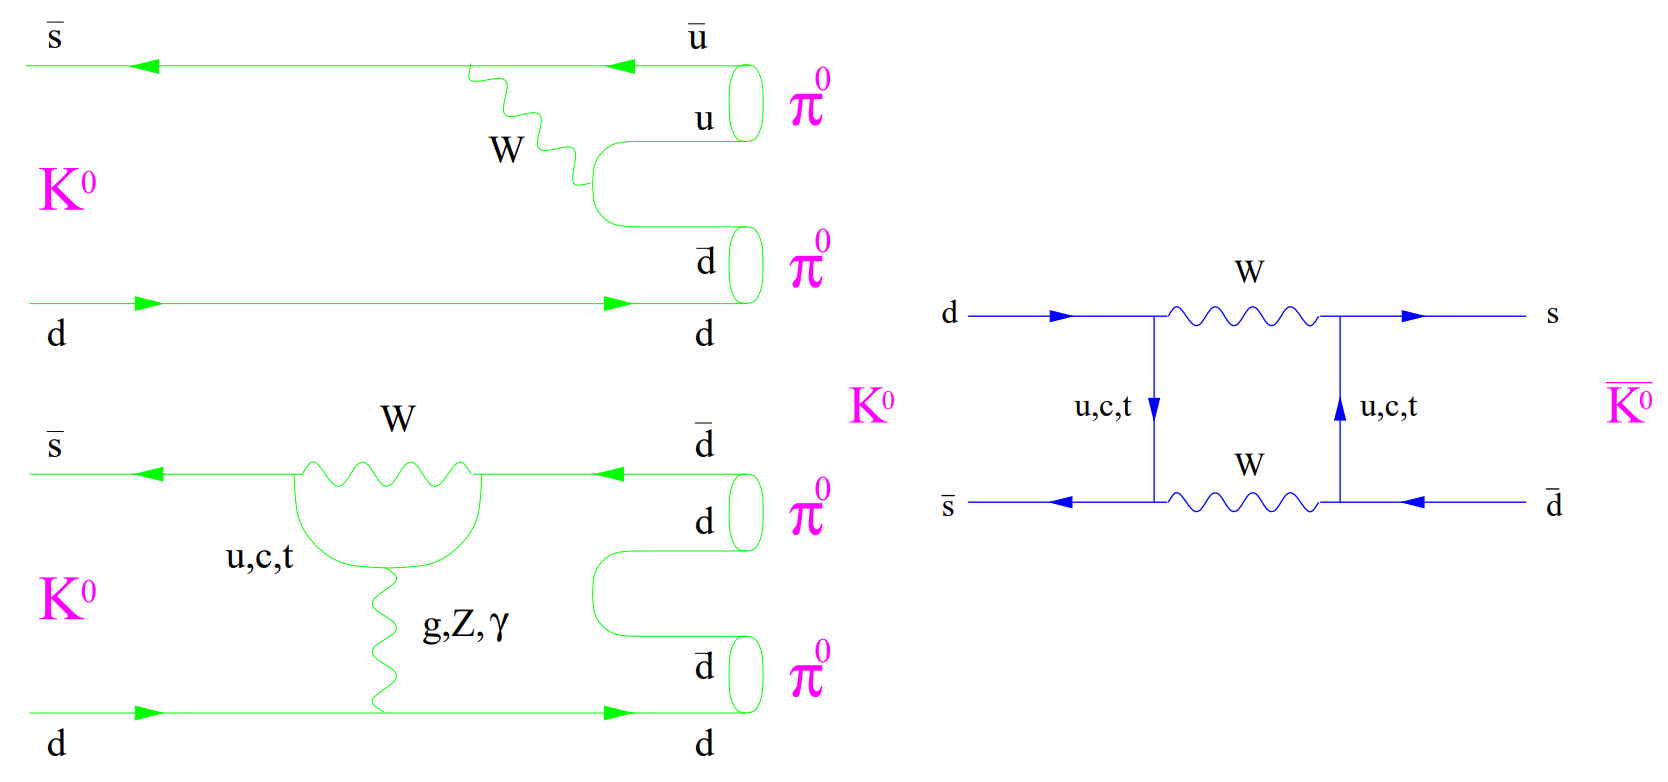
\includegraphics[width=\textwidth]{figures/chapter1-figs/Kaon_CPviolation.png}
    \caption[The left figure shows the “tree” level (top) and “penguin” level (bottom) diagrams responsible for the direct CP in Kaon decays. The right figure shows the “box” level diagrams responsible for the indirect CP in neutral Kaon mixing.]{The left figure shows the “tree” level (top) and “penguin” level (bottom) diagrams responsible for the direct CP in Kaon decays. The right figure shows the “box” level diagrams responsible for the indirect CP in neutral Kaon mixing. Figure taken from \cite{Sozzi2008}.}
    \label{fig:Kaon_decay}
\end{figure}
\clearpage}

The first evidence of CP violation was discovered by the observation of neutral Kaon decay, $K_L^0 \rightarrow \pi^+ \pi^-$, in 1964 \cite{Christenson1964}. This indirect CP violation was attributed to the fact that $K_L$ and $K_S$ mass eigenstates are a mixture of CP even and odd weak flavor eigenstates arising from ``box" type interaction diagrams as shown in \cref{fig:Kaon_decay} \cite{PDG2022, Bigi2009, Sozzi2008}. Direct CP violation was also discovered in the direct Kaon decays, where a tiny difference of $\left( 1.6 \pm 0.2 \right) \times 10^{-3}$ between the observed decay amplitude ratio of $ K \rightarrow \pi^+ \pi^- $ and $ K \rightarrow  \pi^0 \pi^0 $ decay modes was reported by NA48 \cite{Batley2002} and KTeV \cite{Abouzaid2011} experiments. In the SM, this direct CP violation happens due to the mixing between ``tree" type interaction diagrams and ``penguin" type interaction diagrams in Kaon decays \cite{PDG2022, Bigi2009, Sozzi2008} as shown in \cref{fig:Kaon_decay}. These observations have been crucial in understanding the weak interaction as well as predicting the three generational flavor structure of the quarks. Additionally, these results also provided the absolute definition for the difference between matter and anti-matter. Recently, even larger CP violation has been measured in B-mesons \cite{Aubert2001, Abe2001, Aaij2013} and D-mesons \cite{Aaij2019}. These observations are useful in providing a check of the expected SM CKM matrix flavor unitarity as well as the expected SM mechanisms of CP violation, which are difficult to calculate for heavy flavoured mesons due to interference from many ``tree" and ``penguin" type interaction diagrams \cite{PDG2022}. Despite this robust experimental effort over the years to explore CP violation, there has been no indication of BSM physics.

CP violation is also possible in the lepton sector via the CP violating phase in the neutrino weak flavor mixing governed by the Pontecorvo–Maki–Nakagawa–Sakata (PMNS) matrix \cite{Maki1962, Agostini2023}. Although statistics limited, recent global fits on data from neutrino oscillation experiments hint at CP-violation effects in neutrino oscillations \cite{deSalas2021, Gonzalez-Garcia2021, Denton2021}. The future neutrino oscillation experiments of DUNE \cite{Abi2020} and Hyper-Kamiokande \cite{DiLodovico2017} are expected to provide high statistics constraints on CP violation in neutrino oscillations. Additional CP violating phases are possible in the PMNS matrix if neutrinos are discovered to be Majorana particles \cite{Agostini2023}. Although all searches have yielded a null result thus far, highly sensitive experimental searches for neutrinolesss double beta decay, which implies a Majorana neutrino, are being planned in the upcoming experiments of CUPID\cite{Cupid2019}, LEGEND-1000\cite{Legend2021}, nEXO\cite{Adhikari2022}, NEXT\cite{Adams2021}, SNO+\cite{Albanese2021} and more. 

Since T violation implies CP violation via the CPT invariance, direct observations of T violation can also reveal possible BSM physics. The CPLEAR experiment observed T violation in the neutral Kaon oscillation probabilities of $ K^0 \leftrightarrow \Bar{K^0}$ by measuring a small asymmetry in the time dependent decay rate of the semi-leptonic Kaon decays \cite{Angelopoulos1998}. BABAR experiment has also observed T violation through the exchange of initial and final states in the entangled neutral B mesons by measuring a time difference between the two B meson decays \cite{Lees2012}. These result are however difficult to interpret and distinguish between T-violating and CP-violating effects due to the presence of direct CP violation in Kaons and B meson from the SM, let alone BSM.

High precision measurements have played a major role in searches for new physics. They allow for empirical testing of theories and models that attempt to explain natural phenomena. The idea being, if the measured result shows an anomalous deviation relative to theory that is larger than the experimental precision, then the theory is limited and must be expanded upon with new physics to explain the anomaly. While anomalous observations from high precision experiments provide hints towards the possible energy/mass scales of the new physical phenomena, the existence of said new physical phenomena is then confirmed by collider experiments operating at the direct on-shell center of mass energies.  

The SM has been very successful in predicting the physical properties of the subatomic particles. For instance, the magnetic moment of the electron has been measured to 0.13 part per trillion level \cite{Fan2023}, confirming the efficacy of the SM, which is used to calculate the magnetic moment of the electron by taking into account the higher order virtual loops of the quantum fields responsible for the, in so far known, matter and photon interactions. Despite the high efficacy of the SM, recent measurement of the anomalous magnetic moment of the muon to 0.46 parts per million by Fermilab Muon g-2 experiment \cite{Abi2021} indicates a $4.2\sigma$ tension with the SM \cite{Aoyama2020}. This may indicate that new beyond Standard Model (BSM) physics is needed to explain the discrepancy\footnote{It has been pointed out that issues with the theoretical calculations of the anomalous magnetic moment of the muon may be the source of this discrepancy \cite{Borsanyi2021}.}.

Electric dipole moments (EDM) of fundamental particles are a clear T violation phenomena and can also be used as tests of CP violation, assuming CPT invariance \cite{Khriplovich1997, Chupp2019}. Just as high precision searches of the anomalous magnetic moments of fundamental particle can indicate possible BSM physics, high precision searches for EDMs may also hint at BSM physics \cite{Pospelov2005, Ginges2004, Chupp2019, Engel2013}. Even though there have been no experimental observations of a non-zero EDM of an elementary particle to date, high precision experiments have placed stringent limits on the EDMs of the electron \cite{Roussy2023}, muon \cite{Bennett2009}, proton (from theory and the EDM of $^{199}$Hg atom) \cite{Sahoo2017}, and neutron \cite{Abel2020}. New experimental efforts are underway with the goal of improving the current sensitivities on the EDM \cite{Chupp2019}. The remainder of this chapter will focus the neutron's EDM (nEDM). 

%Neutrons are one of the simplest systems to search for BSM physics. They are electrically neutral and can be mass produced. 

\section{Theory of the nEDM}

The EDM of a particle is defined as 
\begin{equation} \label{eq:dipole}
\vec{d_e}=\int \Vec{x} \rho(\Vec{x})  d\Vec{x}
\end{equation}
where $\Vec{x}$ is the orientation of dipole vector, $\rho$ is the charge density. For an uncharged particle like neutron, a non-zero EDM would indicate an asymmetric charge distribution with a net charge of zero. From the Wigner-Eckart Theorem, the orientation of a particle's EDM is set by the spin orientation, $\Vec{s}$, of that particle. From this, the interaction Hamiltonian of an electric and magnetic dipole moment under the influence of an electric and magnetic field can be stated as:
\begin{equation} \label{eq:int_hamilt_m}
    H_m = -d_m \Vec{s} \cdot \vec{B}
\end{equation}    
\begin{equation} \label{eq:int_hamilt_e}
    H_e = -d_e \Vec{s} \cdot \vec{E}
\end{equation}
The P and T violating behavior of \cref{eq:int_hamilt_m} and \cref{eq:int_hamilt_e} can be seen as:
\begin{equation}
    H_m = -d_m \Vec{s} \cdot \vec{B} \xrightarrow[]{P} -d_m( \Vec{s} ) \cdot ( \vec{B} ) = H_m
\end{equation}
\begin{equation}
    H_m = -d_m \Vec{s} \cdot \vec{B} \xrightarrow[]{T} -d_m( -\Vec{s} ) \cdot ( -\vec{B} ) = H_m
\end{equation}
\begin{equation}
    H_e = -d_e \Vec{s} \cdot \vec{E} \xrightarrow[]{P} -d_e( -\Vec{s} ) \cdot ( \vec{E} ) = -H_e 
\end{equation}
\begin{equation}    
    H_e = -d_e \Vec{s} \cdot \vec{E} \xrightarrow[]{T} -d_e( \Vec{s} ) \cdot ( -\vec{E} ) = -H_e
\end{equation}
As stated earlier, T violation implies CP violation as well, under the assumption of CPT invariance. This fundamental EDM is different from EDM's of polarized atoms and molecules, which are caused by the presence of mixing of their energetically degenerate ground state. The exclusion principle forbids a spin-1/2 particle like the neutron to possess an energetically degenerate ground state, therefore, the existence of a non-zero nEDM requires CP violation. Additionally, this fundamental EDM is also different from the induced electric polarizability of the neutron under application of an electric field. Assuming the induced EDM as $D = 4\pi \epsilon_0 \alpha_n E$, the electric polarizability of the neutron, $\alpha_n$, has been measured to be $(11.8 \pm 1.1) \times 10^{-4}$ fm$^{3}$ \cite{PDG2022, Myers2014}. To put that in perspective, an electric field of 100 kV/cm will induce an EDM, always aligned with E, at the level of $10^{-31}$ e$\cdot$cm, much smaller than the current or planned limit on the fundamental EDM.

\subsection{nEDM from Standard Model}

\subsubsection{The electro-weak sector:}

Since the neutron is made up two up quarks and one down quark, the discussion of nEDM must start at the quark level. The quark EDM appears only at the three loop level diagrams in the SM with the dominating effect due to the exchange of two W bosons and one gluon \cite{Czarnecki1997, Chupp2019}. \cite{Czarnecki1997} calculates the values of the up quark EDM, $d_{u}$, and the down quark EDM, $d_{d}$ to be:
\begin{equation}
    d_{u} \approx -0.15\times10^{-34} \ e \cdot cm 
\end{equation}
\begin{equation}
    d_{d} \approx -0.7\times10^{-34} \ e \cdot cm
\end{equation}
The neutron is composed of three ``valence" quarks with different color charges, $udd$, and a ``sea" of gluons and quark-antiquark pairs. Naively, the valence quark contribution becomes:
\begin{equation}
    d_{n} = \frac{4}{3}d_{d} + \frac{1}{3}d_{u} \approx -0.9\times10^{-34} \ e \cdot cm
\end{equation}
The largest SM contribution to $d_n$ does not come from quark EDMs, but from a long distance P-odd/T-odd meson-exchange ``strong penguin" diagram as shown in \cref{fig:penguin} \cite{Seng2015, Chupp2019}. This leads to an expected SM nEDM value of:
\begin{equation}
    d_{n} = (1-6) \times 10^{-32} ~ e \cdot cm
\end{equation}

\afterpage{
\begin{figure}
    \centering
    \begin{minipage}{0.50\textwidth}
        \centering
        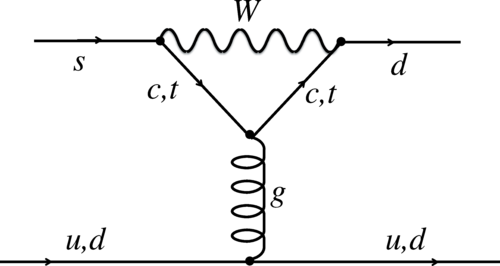
\includegraphics[width=0.9\textwidth]{3_loop_level.png} % first figure itself
        \end{minipage}\hfill
    \begin{minipage}{0.50\textwidth}
        \centering
        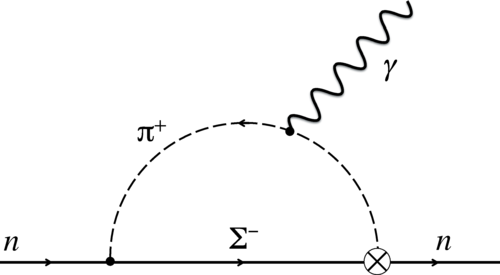
\includegraphics[width=0.9\textwidth]{chiral_loop.png} % second figure itself
        \end{minipage}
    \caption[The 3-loop level ``strong penguin'' diagram at the crossed-circle point of CP-odd meson-nucleon-nucleon interaction giving the effective SM CP-violation.]{The 3-loop level ``strong penguin'' diagram at the crossed-circle point of CP-odd meson-nucleon-nucleon interaction giving the effective SM CP-violation. Figure taken from \cite{Chupp2019}.}
    \label{fig:penguin}
\end{figure}
\clearpage}

\subsubsection{The strong sector:}
CP violation in the strong sector is also possible due to the $\Bar{\theta}$-term in the SM Quantum Chromodynamics (QCD) Lagrangian. 
\begin{equation}
    %\mathcal{L}=-\frac{1}{4}F_{\mu\nu}F^{\mu\nu}-\frac{n_fg^2\theta}{32\pi^2}F_{\mu\nu}\Tilde{F}^{\mu\nu}+\Bar{\psi}(i\gamma^\mu\mathcal{D}_\mu-me^{i\theta^{'}\gamma_5})\psi
    \mathcal{L}= \Bar{{\theta}}\frac{g^{2}_{s}}{32\pi^2}G^{a}_{\mu\nu}\Tilde{G}^{\mu\nu}_{a}
    \label{eq:qcd_theta}
\end{equation}
where $g_s$ is the strong force coupling constant and $G^{a}_{\mu\nu}$ and $\Tilde{G}^{\mu\nu}_{a}$ are the gluon field strength tensors, whose product violates CP symmetry \cite{Pospelov1999, Crewther1979}. Thus experimental constraints on nucleon nEDMs can be used to set upper limits on $\Bar{\theta}$ \cite{Pospelov1999, Crewther1979}. The nEDM in units of $\Bar{\theta}$ is given by:
\begin{equation}
    d_{n} \approx -(0.9 - 1.2) \times 10^{-16} \Bar{\theta} \; e \cdot cm
\end{equation}
so the current experimental limit implies $\Bar{\theta} \lesssim 10^{-10}$, neglecting hadronic uncertainties \cite{Seng2015}. This smallness of $\Bar{\theta}$ gives rise to the strong-CP problem. \cite{Peccei1977, Peccei1977a, Hooft1976a} propose a solution to this problem by introducing a global $U(1)$ chiral symmetry however, the breaking of such a symmetry leads to a new light pseudoscalar boson, called the axion. Although not yet observed, the axion is postulated to be a potential constituent candidate for dark matter with broad experimental efforts in search. 

%Furthermore, coupling of axion like particles to nucleons have been  The axion’s anomalous coupling to gluons induces, at energies below the confinement scale of QCD, a model-independent coupling of the axion to the operator giving rise to the EDM of the nucleon (N)

\subsection{nEDMs from Beyond the Standard Model}

Considering potential phenomena at energy scales well above the electroweak scale, BSM models proposed in \cite{Dubbers2011, Chupp1987} could introduce new CP and T violating interactions. Most of these BSM scenarios involve new particles with masses , $M_{BSM}$, well above the electroweak scale, giving rise to new couplings and further CP-violating phases, $\delta_{BSM}$ , which can, in principle, increase the magnitude of nEDM as (on a dimensional analysis basis) \cite{Alarcon2022, Chupp2019, Morrissey2012, Dubbers2011, Engel2013}: 
\begin{equation}
    d_{n} \sim 10^{-26}\; e \cdot cm\left(\frac{1~TeV}{M_{BSM}}\right)^2 \sin{\delta_{BSM}}
\end{equation}  
So far, measurements at the LHC have produced null results in searches for these BSM massive particles at 13 TeV energies \cite{PDG2022}. Since BSM predicted nEDM is, in principle, much larger than SM prediction, an improvement on the current nEDM limit can place constraints on CP violating BSM mass scales thus offering a complimentary probe to BSM searches at LHC. 

Considering the SM valid at low energy scales, the low energy manifestations of the possible high energy BSM physics can be described through an effective field theory (SMEFT) as:
\begin{equation}
    \mathcal{L}_{eff}^{CP} \approx \mathcal{L}_{SM} +  \underbrace{ \frac{ C^5 }{\Lambda} \mathcal{O}_i(5) + \sum_i \frac{ C_{i}^6 }{\Lambda^2} \mathcal{O}_i(6) + ... }_{\mathcal{L}_{BSM} }
\end{equation}
where $C_i$ encode all of short-distance information and $\Lambda$ is the effective BSM energy scale \cite{Chupp2019}. The leading CP violating operators, $\mathcal{O}_i$, which possibly contribute to nEDM, arise at dimension order six\footnote{Dimension-5 terms are only relevant for neutrino physics \cite{Agostini2023}.} and consist of quark EDMs, chromo-quark EDMs, chromo-gluon EDMs, CP-violating 3 gluon couplings, CP-violating four quark couplings and CP-violating quark-Higgs couplings \cite{Yamanaka2021}. These resulting effective CP-violating operators can be linked to an SMEFT that only contains the relevant hadronic physics and be solved for. Lattice QCD (LQCD) has shown promise to obtain ab initio QCD-based results. So far, LQCD has focused on calculating the nEDM from the quark EDMs and the QCD $\Bar{\theta}$ term in \cref{eq:qcd_theta} \cite{Alexandrou2021, Bhattacharya2021}. Higher-dimensional operators such as the quark and gluon chromo-EDMs are also being calculated. \cite{Shindler2021} provides a more thorough review of these approaches.
%(see Shindler [51] for a recent review , [27,28,46,47 in pdg]).

\subsection{Interpreting the nEDM}

Even though nEDM is a useful probe for CP violating physics, it is insufficient to explain the fundamental CP violating mechanism responsible for the baryon asymmetry problem. Further searches for the EDMs of multiple systems (quarks, leptons, nucleons, light nuclei, atoms and more) have to performed, along with their theoretical calculations, to understand the manifestation of fundamental CP violation in the effective energy hierarchy of these systems \footnote{As compared to other subatomic particles, experiments on free neutrons are a little less challenging to perform since neutrons are electrically neutral \cite{Chadwick1932} and thus, not influenced by electromagnetic fields, and they can be mass produced in reactors as well as spallation sources.} \cite{Chupp2019}. A schematic illustration of how EDMs can be used to search for fundamental CP violation sources is shown in \cref{fig:nEDM_Globalpic}. The collective analysis of the CP violation from EDMs as well as the CP violation from the CKM and PMNS sectors will provide a more global perspective on the true CP violating phenomena at the fundamental level. 

\afterpage{
\begin{figure}
    \centering
    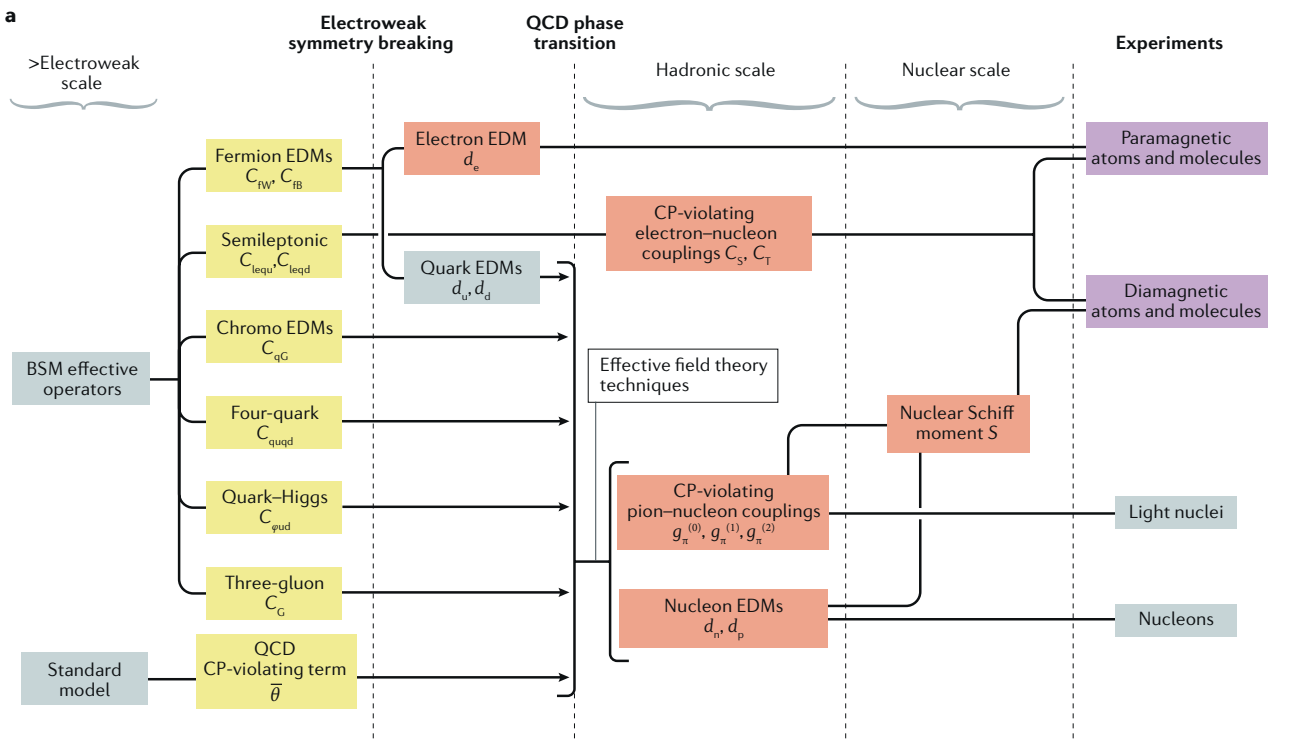
\includegraphics[width=\textwidth]{figures/chapter1-figs/EDM_interp2.png}
    \caption[A flow diagram illustrating the effective energy hierarchy based global analysis of fundamental BSM CP-violating interactions manifesting in observable low-energy CP-violating phenomena.]{A flow diagram illustrating the effective energy hierarchy based global analysis of fundamental BSM CP-violating interactions manifesting in observable low-energy CP-violating phenomena. Figure taken from \cite{Cairncross2019}.}
    \label{fig:nEDM_Globalpic}
\end{figure}
\clearpage}

\section{Principles of nEDM Measurement}

The primary method for measuring the nEDM is to look for a change in the Larmor precession frequency of neutrons, $\omega_n$, with a magnetic moment, $\mu_n$, and an electric dipole moment, $d_n$, under the application of a large static electric field, $E_0$, parallel and antiparallel with respect to a small static magnetic field, $B_0$ \cite{Ahmed2019}. This is illustrated in \cref{fig:Larmor} and can be stated as:
\begin{equation} \label{eq:larmor}
\omega_n=\frac{-2\left(\mu_n B_0\pm d_n E_0\right)}{\hbar}
\end{equation}
The statistical uncertainty of the nEDM measurement depends on the strength of the applied electric field, $E_0$, the number of neutrons observed, $N$, and the precession measurement time, $\tau$, \cite{Ahmed2019} as:
\begin{equation} \label{eq:uncertainty}
\sigma_{d_n}=\frac{\sqrt{2} \hbar}{4 E_0 \tau \sqrt{N}}
\end{equation}
The next generation of nEDM experiments aiming to improve upon nEDM limit optimize the quantity $ E_0 \tau \sqrt{N} $.

\afterpage{
\begin{figure}
    \centering
    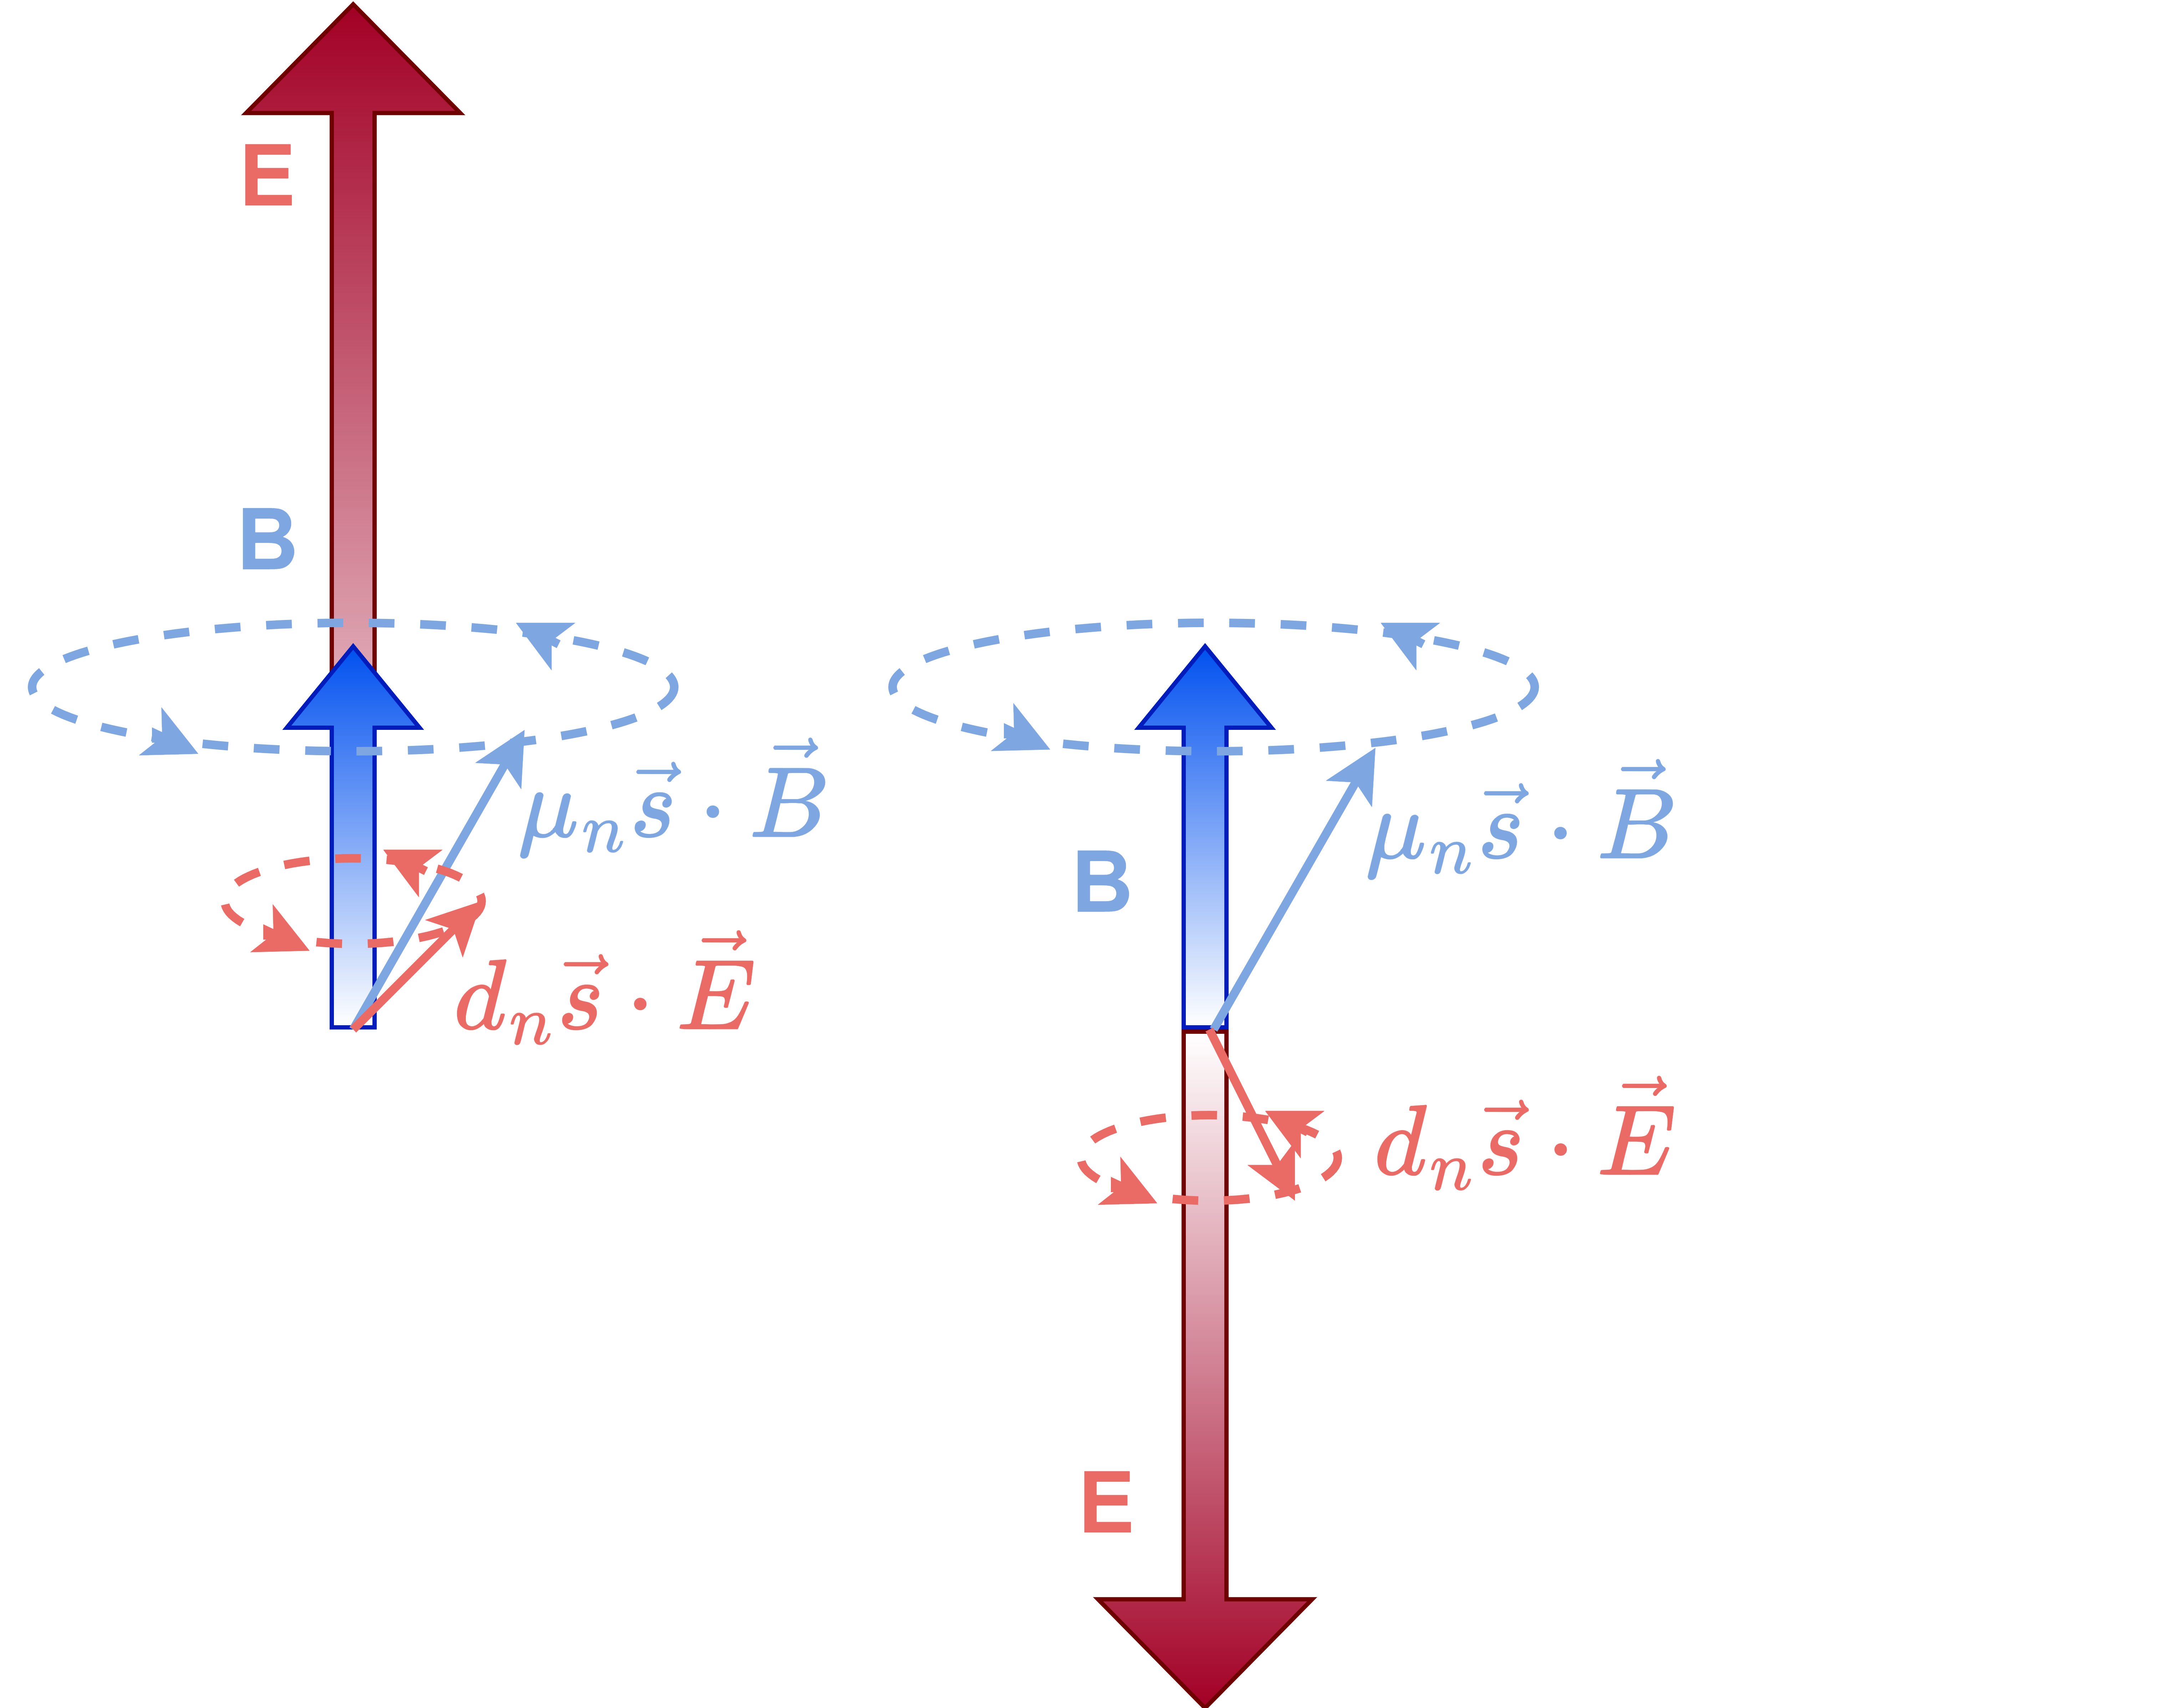
\includegraphics[width=0.75\textwidth]{figures/chapter1-figs/Larmor_precession.png}
    \caption[A cartoon illustrating the Larmor precesion of the neutron with a magnetic moment and an electric dipole moment under the application of an electric field, E, parallel and antiparallel with respect to a magnetic field, B.]{A cartoon illustrating the Larmor precesion of the neutron with a magnetic moment and an electric dipole moment under the application of an electric field, E, parallel and antiparallel with respect to a magnetic field, B.}
    \label{fig:Larmor}
\end{figure}
\clearpage}

The first experiment to look for nEDM took place at the neutron beam of the Oak ridge graphite reactor, where the nEDM from Larmor precession was measured using the method of separated oscillatory fields \cite{Ramsey1950, Purcell1950, Smith1957}. This neutron beam method has mostly been abandoned due to the discovery of a systematic effect associated with the motional magnetic field prohibiting the sensitivity reach towards the expected nEDM \cite{Dress1977}. Despite the large counting statistics advantage of neutron beams, these early measurements pointed out that competitive precision can be obtained with the slower Ultracold Neutrons (UCN), which can be stored for longer periods of time, and therefore, allow for a longer neutron precession measurements \cite{Golub1991}.

UCNs are essentially defined by the materials used to store them \cite{Golub1979a, Golub1991}. The interaction of UCN (Kinetic energy (K.E.) $\sim$ 200 neV, $\lambda$ $\sim$ 100~\AA, T $\sim$ mK) with material surfaces is characterized by an effective potential energy, $V_F$ , which is set by the coherent scattering length of neutrons from many nuclei in the storage material and is positive for most materials \cite{Fermi1936, Fermi1947, Golub1979a, Golub1991}. Neutrons with K.E. $<$  $V_F$ are repelled from the chamber walls, undergoing total external reflection and effectively getting confined \cite{Zeldovich1959, Steyerl1969, Lushchikov1969, Golub1979a,  Golub1991}. This storage allows for long precession and observation times of several hundred seconds and hence, precise measurements of nEDM \cite{Golub1991}.

Improving upon nEDM limit by optimizing the quantity $ E_0 \tau \sqrt{N} $ is difficult. Despite the storage advantage of UCNs, the limiting factor for nEDM sensitivity is achieving a high UCN density (UCN/cm$^3$). By employing the neutron superthermal scattering method from superfluid helium or solid deuterium, new UCN sources have been and are being developed for nEDM experiments to provide high UCN densities and hence high statistics \cite{Golub1975, Golub1979a, Golub1991}. The strength of the electric field is typically limited by the field emission electrons at the electrostatic boundaries of the electrodes. The precession time is limited from various UCN loss mechanisms with the UCN storage/transport material.

In natural units, the magnetic moment of neutron, $|\mu_n|$ = 0.332 GeV$^{-1}$ , is 14 orders of magnitude bigger then the most recent nEDM limit, $|d_n|$ $<$ 4.58 $\times$ 10$^{-15}$ GeV$^{-1}$ \cite{Codata2021, PDG2022}. To put that in perspective, the precession frequency from the neutron's magnetic moment in the 50 µT Earth’s magnetic field is around 250 Hz (corresponding to $10^{-12} eV$) while the current limit of nEDM $10^{-26}$ e$\cdot$cm in the 3 MV/m breakdown electric field of the Earth’s atmosphere causes a precession of 24 nHz (corresponding to $10^{-22} eV$). This illustrates that the precession signal from the magnetic interaction overwhelmingly dominates the precession from the nEDM. If the magnetic fields are kept highly uniform, the dominating magnetic interaction can be measured and accounted for. Therefore, nEDM experiments necessitate meticulous control of magnetic field fluctuations and utilize highly advanced magnetics (magnetic shielding and magnetic field coil geometries) and atomic comagnetometry (spin polarized species that occupy the same volume as the stored UCN, thus providing the a live average of the magnetic field experienced by the stored UCN) to monitor the stability and uniformity of the magnetic field \cite{Alarcon2022}. Nevertheless, this can only be done so well and systematic effects from magnetic field non-uniformities are bound to arise. The geometric phase effect, caused by the combination between non-uniformity of the magnetic field and the motional magnetic field, is, at present, the largest systematic effect limiting the nEDM sensitivity \cite{Pendlebury2004}.    

Improvements to UCN storage technology has been made for nEDM measurements at the Institut Laue-Langevin (ILL) \cite{Baker2006} and the Petersburg Nuclear Physics Institute (PNPI) \cite{Serebrov2014}. The most recent experimental limit  of $\mid d_n \mid < 1.8 \times 10^{-26}$ e$\cdot$cm (90\% C.L.) was set by the Paul Scherrer Institut (PSI) in 2020 \cite{Abel2020} using a room temperature ILL style separated oscillatory fields nEDM apparatus with an external UCN source and atomic magnetometry to account for the geometric phase systematic effect. The PSI nEDM experiment was able to achieve an average UCN density of 2 UCN/cm$^{-3}$, an electric field of 10 kV/cm and a precession time of $\sim$180 seconds. The historical advancement of the nEDM upper limit is shown in \cref{fig:nEDM_history}. The figure shows that further experimental searches are needed to push the upper limit of the nEDM in order to constraint BSM predictions.  

\afterpage{
\begin{figure}
    \centering
    \includegraphics[width=\textwidth]{figures/chapter1-figs/nEDMupperbounds_3.png}
    \caption[A history plot of the measured nEDM upper limits.]{A history plot of the measured nEDM upper limits. The colored regions show the nEDM predicted values from the SM and BSM predictions \cite{Chupp2019}. Some key nEDM experiments throoughout history are highlighted. The latest upper limit measured in and 2020\cite{Abel2020} is also shown. The horizontal green line indicates the projected goal of nEDM@SNS experiment \cite{Ahmed2019}. A more complete list of all the nEDM experiments performed so far can be found in \cite{Lamoreaux2009} and \cite{PDG2022}.}
    \label{fig:nEDM_history}
\end{figure}
\clearpage}

\section{Outline of Dissertation}

This chapter impresses the need for new searches of CP violating phenomena to explain the baryon asymmetry of the universe. The chapter also describes how the nEDM is a powerful CP violating phenomena that can perhaps elucidate the baryon asymmetry problem. Now that the physics is well motivated, a new experimental search along with an the associated R\&D project are described in the following chapters:
\begin{itemize}
    \item \Cref{ch:nEDM} describes the nEDM@SNS experiment, which aims to reach a nEDM sensitivity of a few $\times~10^{-28}$ e$\cdot$cm. In this experiment, polarized UCNs, polarized $^3$He in a solution of superfluid $^4$He will used \cite{Ahmed2019}. Technical details about the innovative measurement techniques as well as the experimental apparatus design are discussed.
    \item \Cref{ch:polHe} describes the neutron polarimetry technique, where polarized $^3$He is used to perform neutron spin polarization analysis. The first half of the chapter is dedicated to the optical pumping techniques used to polarize $^3$He and the latter half is describes the design and proof of demonstration of an in situ polarized $^3$He system for neutron spin analysis.   
    \item \Cref{ch:PT} describes the neutron polarization and transmission measurements, a preliminary R\&D effort, to verify the design of the cryomagnet of the nEDM@SNS experiment. The uniaxial neutron polarimetry experimental setup at the monochromatic neutron SNS beamline 13A is presented followed by results of the data taking campaign in the summer of 2023. Lastly, Small Angle Neutron Scattering measurements on the beam windows materials are presented.   
    \item \Cref{ch:conclusions} briefly summarises and discusses the main neutron polarization and transmission results detailed in this dissertation and then presents future plans for an upgraded setup.
\end{itemize}
    %!TEX root = ../thesis.tex
%*******************************************************************************
%****************************** Second Chapter *********************************
%*******************************************************************************

\chapter{The nEDM@SNS Experiment}
\label{ch:nEDM}


\ifpdf
    \graphicspath{{figures/chapter2-figs/}{Chapter2/Figs/PDF/}{Chapter2/Figs/}}
\else
    \graphicspath{{Chapter2/Figs/Vector/}{Chapter2/Figs/}}
\fi

\afterpage{
\begin{figure}
    \centering
    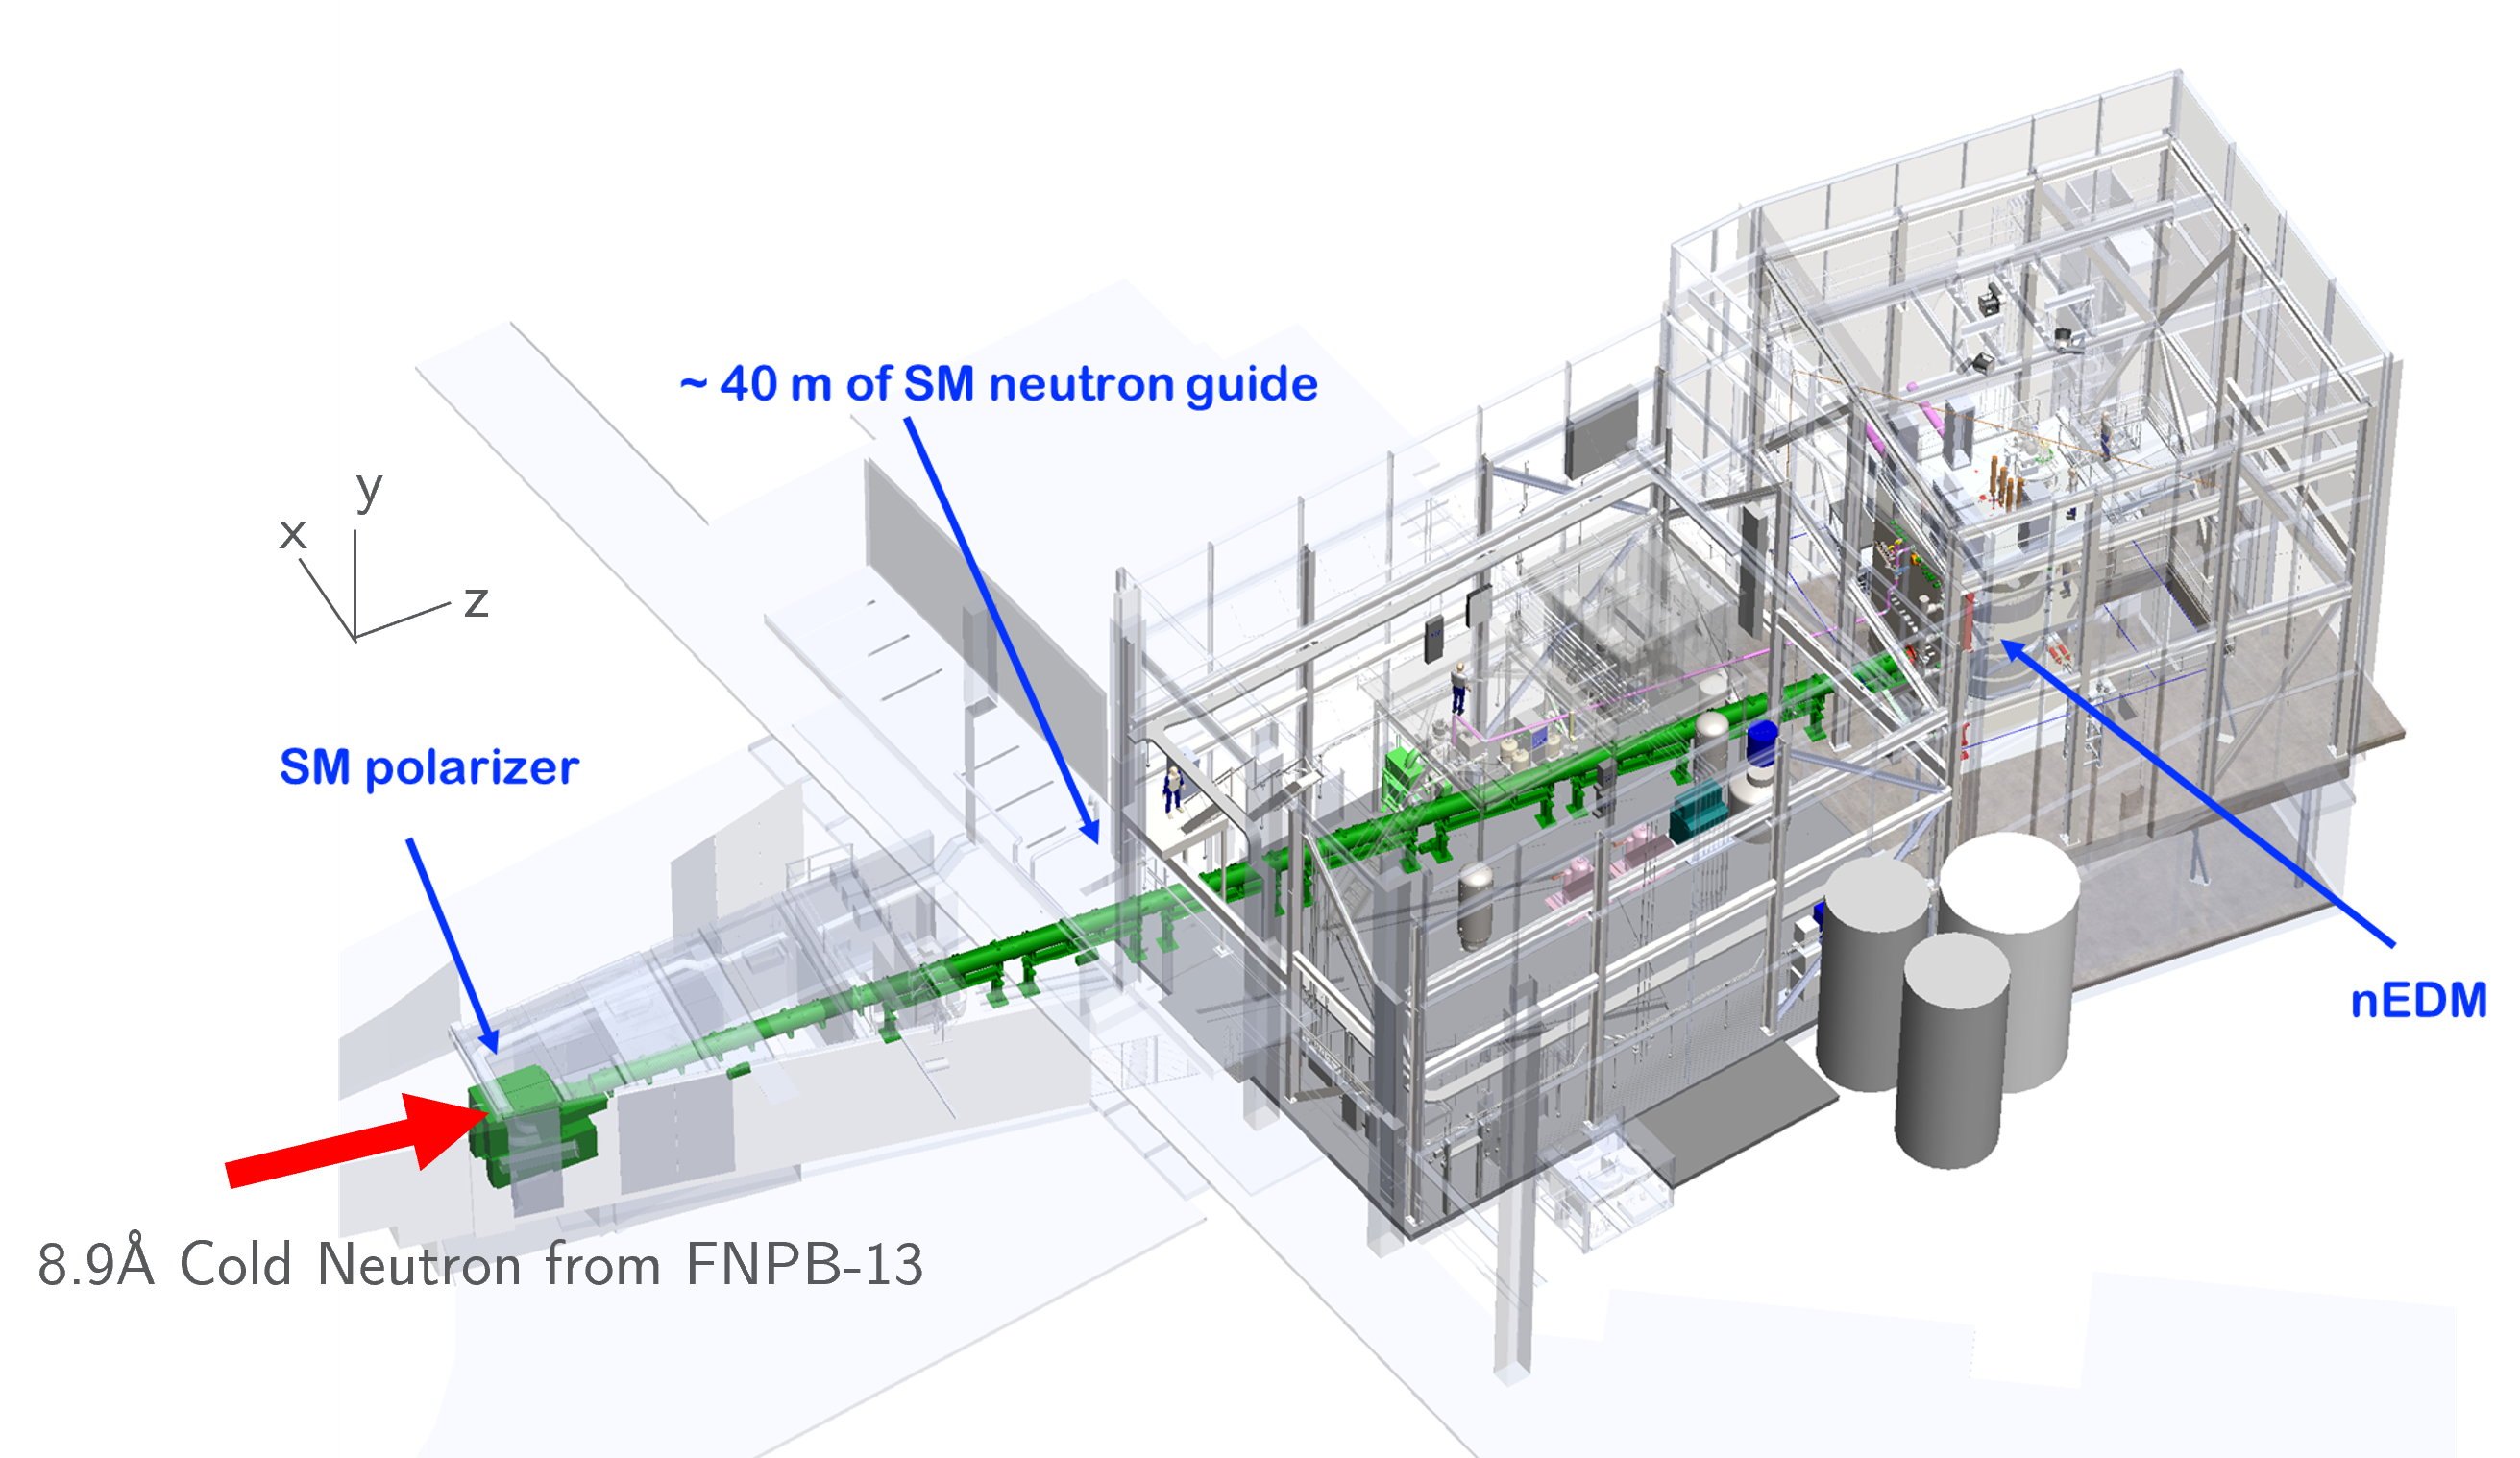
\includegraphics[width=1\textwidth]{figures/chapter2-figs/nEDM_SNS_entire_experiment.png}
    \caption{Schematic overview of the nEDM@SNS experimental apparatus at the Spallation Neutron Source FNPB 13. Figure courtesy of Wolfgang Korsch of the nEDM@SNS collaboration.}
    \label{fig:full_nEDM@SNS}
\end{figure}
\clearpage}

It is clear from the theoretical motivation and the experimental limitations mentioned in \cref{ch:intro} that pioneering experiments are needed to push the sensitivity for the nEDM. In this chapter, the nEDM@SNS experiment, a novel cryogenic apparatus with the goal of improving the nEDM sensitivity, housed at the Spallation Neutron Source (SNS), is described. A schematic overlay nEDM@SNS experiment is shown in \cref{fig:full_nEDM@SNS}. The overall physics of the experiment, the measurement scheme to achieve the expected sensitivity and the major component of the experimental apparatus are described.

\section{Overview}

This experiment, based on the a concept proposed in Ref.~\cite{Golub1994}, makes use of polarized UCN's and polarized $^3$He in superfluid $^4$He. The superfluid $^4$He is used to produce a high density of UCNs in a pair of measurement cells. With this in situ UCN production, the problems of UCN intensity loss that take place for nEDM experiments with external UCN source are avoided. The experiment, uses polarized $^3$He, as a co-magnetometer as well as a live in situ UCN spin analyzer. By contrast, the separated oscillatory fields NMR techniques used in other nEDM experiments analyze the spin precession externally and at the end of the measurement period, leading to statistical sensitivity loss. The superfluid $^4$He is also used as a dielectric insulator allowing for significantly higher electric fields \cite{Ito2016}. These innovative features provide the experiment's ultimate statistical sensitivity for the nEDM as 3-6~$\times$~10$^{-28}$~e~$\cdot$~cm, two order of magnitude better compared to the current nEDM sensitivity.

\afterpage{
\begin{figure}
    \centering
    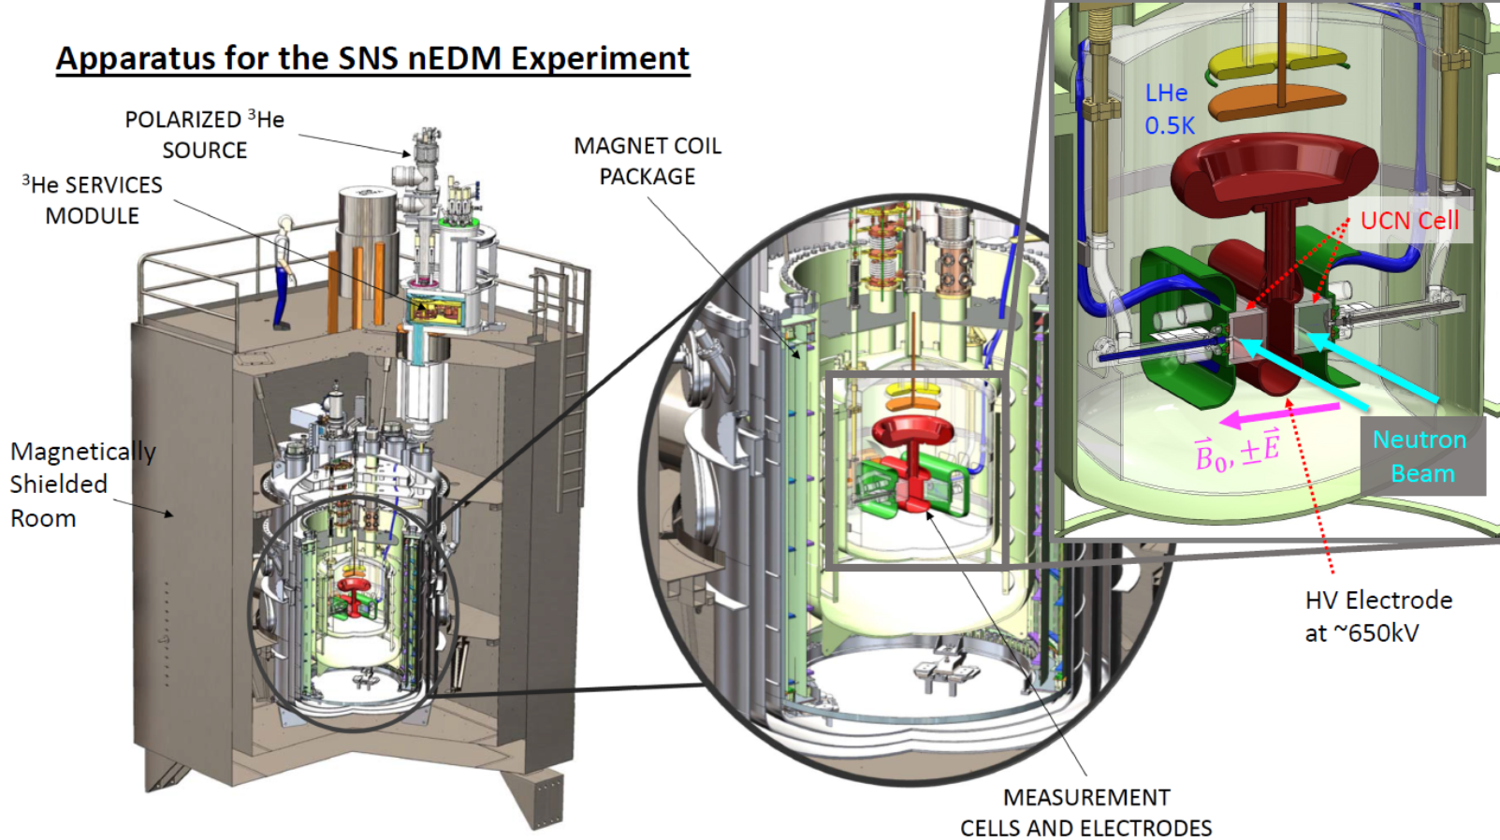
\includegraphics[width=1\textwidth]{figures/chapter2-figs/nEDM_SNS_detail_experiment.png}
    \caption{A detailed schematic overview of the nEDM@SNS experimental apparatus.}
    \label{fig:nEDM@SNS_detail}
\end{figure}
\clearpage}

%The experiment will produce UCN via super-thermal scattering of incoming polarized cold neutrons ($\lambda$ $\sim$ 8.9 \AA) off of phonons in superfluid $^4$He \cite{GOLUB1977337}. UCN's can be confined to a storage volume made of materials with a Fermi potential less than 165 neV. With now experimentally realizable cryogenic temperatures (T $<$ 0.7K) and appropriate materials for storage cells, UCNs can be stored in $^4$He for long periods of time. This, coupled with the fact that superfluid He has large dielectric breakdown strength and hence allows for application of large electric fields \cite{ITO16}, maximizes E$_0$, $\tau$ and $N$ in eq. \ref{eq:uncertainty}. nEDM@SNS will apply B$_0$ = 30 mG and E$_0$ = 75 kV/cm to measure the larmor frequency in eq. \ref{eq:larmor}.

%$^3$He has a spin-dependent neutron absorption cross section, 5300 barns at 1.8\AA \, for anti-parallel neutron and $^3$He spins, increasing as $1/v$, where $v$ is the velocity of neutrons, and nearly zero for parallel neutron and $^3$He spins. For 8.9\AA\ neutrons, the n-$^3$He capture cross section rises to $\sim$26200 barns. For very low concentrations, polarized $^3$He atoms can remain in solution of liquid $^4$He for long periods of time i.e. longer than the neutron's lifetime. The reaction is shown in eq. \ref{abseq}. The energy released from n-$^3$He capture decay products is transferred to the surrounding superfluid $^4$He, which produces ultraviolet (80 nm) scintillation light. Because of the spin dependence of the neutron-$^3$He absorption cross section, the absorption rate of n-$^3$He precessing system is proportional to $1-P_nP_3\cos{\theta_{n3}(t)}$, where $\theta_{n3}(t)$ is the time-dependent angle between UCN and $^3$He polarization, $P_n$ and $P_3$, respectively. The scintillation light will be utilized as the detection mechanism for this variation in n-$^3$He absorption rate. The fact that nEDM@SNS uses in situ spin analysis techniques provide a large increase is statistical sensitivity compared to nEDM experiments that use external spin analysis systems.
%\begin{equation}
%n + {^3He} \rightarrow p+{^3}H+765 \ keV
%\label{abseq}
%\end{equation}
%According to eq. \ref{eq:larmor}, changes in the Larmor frequency, due to the magnetic interaction of $\mu_n$ with magnetic field fluctuations, will decrease the sensitivity of nEDM. Therefore, the nEDM@SNS sensitivity goal necessitates meticulous control of magnetic field fluctuations. Even under such control, magnetic field gradients are expected but can be taken into account using magnetometry. In principle, this magnetometer should provide the average magnetic field over the volume where the neutron precession is taking place. Since the polarized $^3$He has a rapid diffusion time \cite{}, will be exposed to the same magnetic field as UCNs, will be occupying the same volume as the UCN and because the static electric dipole moment of $^3$He is highly suppressed from electron screening \cite{FLAM07}, nEDM@SNS experiment will utilize polarized $^3$He as a co-magnetometer as well. 

%nEDM@SNS will use two frequency measurement techniques. The first method will measure an electric field dependent shift in the scintillation beat frequency. Electric and magnetic fields will be applied to the storage cell parallel to the initial polarization. A $\pi/2$ flip will rotate the spins into a plane perpendicular to the fields. The precession frequency of $^3$He will be measured using SQUID sensors. Since there is a 10\% difference in the gyromagnetic ratios of UCN ($\gamma_n$), and $^3$He ($\gamma_3$), the variation in scintillation rate will be the beat frequency $\Delta\omega = B_0 (\gamma_n - \gamma_3)$. 
%\begin{equation}
 %   \omega_{n3} = \left(\gamma_n - \gamma_3\right) \frac{\omega_3}{\gamma_3} %\pm \frac{2d_nE_0}{\hbar}
%\end{equation}
%The neutron precession frequency shift can then be extracted if the $^3$He precession frequency is added to the scintillation beat frequency, $\omega_{n3}$.  Thus, using the neutron precession frequency under different directions of the electric field, the nEDM can be extracted. Thus, the polarized $^3$He will act as a live in situ co-magnetometer and spin polarization analyzer,

%The second method, called critical spin dressing, involves applying an AC magnetic field, forcing the UCN and $^3$He to precess at the same effective precession frequency.
%\begin{equation}
 %   \omega_n-\omega_3 = \gamma_nJ_0(x_n)-\gamma_3J_0\left(\frac{\gamma_3}{\gamma_n}x_n\right) = 0
%\end{equation}
%where $J_0$ is the zeroth order Bessel function of first kind and $x_n = \gamma_n \frac{B}{\omega}$, where $B$ and $\omega$ are the magnitude and frequency of applied AC magnetic field. $B$ and $\omega$ can be selectively tuned at critical dressing parameter, $x_n$, such that in the absence of an electric field, $\Dot{\theta}_{n3}(t) = 0 $ therefore the scintillation rate will be constant. In the presence of an electric field and a non-zero nEDM, $\theta_{n3}$ will be modified as 
%\begin{equation}
 %   \theta_{n3}(t) = \pm\phi_0 \pm \frac{2J_0(x)d_{n}E}{\hbar}t
%\end{equation}
%where $\phi_0$ is the initial angle between spins, therefore scintillation rate will no longer be constant. This method eliminates the need for $^3$He co-magnetometry.  By utilizing both methods, possible unknown systematic effects can be uncovered.

%The nEDM@SNS experiment will employ a multi-pronged strategy to shield against external fields: external field cancellation coils, room-temperature shielding and superconducting shielding \cite{Ahmed_2019}. As shown in figure \ref{fig:2}, the nEDM magnet cryostat magnet, which surrounds the measurement cells, is made of several concentric layers. The components within the cryogenic magnet package work together to provide shielding and generate magnetic fields that satisfy strict uniformity requirements. Since the nEDM@SNS requires the use of polarized neutrons, therefore, both polarization and transport efficiency of the neutron beam through the cryostat and magnet package windows should be maximized to optimize sensitivity.

%\begin{figure}[p]
 %   \centering
 %   \includegraphics[width=.9\textwidth]{cryogenicapparatus.png}
  %  \caption{A schematic overview of the nEDM@SNS cryostat magnet package. The enlarged section shows the beam windows the incoming polarized neutrons will pass through.}
   % \label{fig:2}
%\end{figure}

\Cref{fig:nEDM@SNS_detail} shows a detailed view of the nEDM@SNS experiment. The Larmor precession measurement, as shown in \cref{eq:larmor}, for the nEDM@SNS experiment will take place inside two measurement cells at the center of the apparatus made of deuterated polystyrene (dPS) plus deuterated tetraphenyl butadiene (dTPB) and acrylic. These cells will be filled with isotopically purified superfluid $^4$He 0.4 K. A highly homogeneous magnetic field, $B_0$, of magnitude 30 mG will be applied along the transverse direction of the measurement cells (parallel to horizontal axis). This field is selected to provide control over the systematic effects arising from magnetic field gradients. Highly Polarized $^3$He ($P_3 \sim 0.98$) , polarized parallel to $B_0$ field, at an isotropic concentration of $x_3 \sim 10^{-10}$ (atomic density of $10^{12}$ cm$^{-3}$), as compared to the natural abundance of $^3$He ($x_3 \sim 10^{-3}$ to $10^{-6}$), will be loaded into the measurement cells. A high voltage electrode, situated in between the two measurement cells and two ground electrodes flanking the measurement cells will be used to provide an electric field parallel to $B_0$ for one cell and antiparallel to $B_0$ in the other cell. The electrodes will provide an expected electric field magnitide of $E_0$ = 75 kV cm$^{-1}$. This high electric field is achievable due to the high dielectric breakdown strength of superfluid helium. 

The measurement cells will be illuminated with polarized 8.9~\AA\ neutrons, which undergo down-scattering in superfluid $^4$He via phonon emission in a process called superthermal scattering, to produce UCNs \cite{Golub1977, Golub1983, Golub1975}. The FNPB neutron beamline 13 with time of flight choppers will be used to provide the monochromatic 8.9~\AA\ neutrons with $\Delta \lambda / \lambda $ of 0.01 to suppress non-UCN converted neutron backgrounds. The monochromatic neutrons will be polarized parallel to the $B_0$ field direction, via a supermirror neutron polarizer ($P_n$ = 0.98) and transported to the measurement cells via neutron guides with spin transport magnetic fields. The UCN polarization is expected to be at the same level since the superthermal process does not cause a change in angular momentum and the spin dependent capture interaction of neutrons and $^3$He eliminates any undesired UCN polarization. The inner walls of the measurement cells will be coated with deuterated polystyrene with a neutron optical potential of $\sim160$ neV. The UCN production rate based on the measurement cell design is expected to be $\approx$ 0.31 UCN cm$^{-3}$ s$^{-1}$.

The UCN density build up, time $\tau_{UCN}$, over the course of the monochromatic neutron beam illumination will be dictated by:
\begin{equation}
    \frac{1}{\tau_{UCN}} = \frac{1}{\tau_{\beta}} + \frac{1}{\tau_{up}} + \frac{1}{\tau_{wall}} + \frac{1}{\tau_{n3}}
    \label{eq:UCN_losstime}
\end{equation}
where:
\begin{itemize}
    \item $\tau_{\beta}$ is the mean neutron $\beta$-decay lifetime of 878 s \cite{PDG2022}. 
    \item $\tau_{up} $ is the UCN loss time from upscattering with the superfluid $^4$He and is expected to be about $ 6 \times 10^4$ s at 0.4 K \cite{Golub1983, Golub1979, Ye2009}.
    \item $\tau_{wall}$ is the UCN loss time from measurement cell wall collisions, and is expected to be $ > $ 2000 s based on the measurement cell design.
    \item $\tau_{n3}$ is the UCN-$^3$He absorption time, which can be chosen to optimize sensitivity.
\end{itemize}
Based on this UCN built up time, the maximum achievable UCN density in each cell is expected to be $\approx$ 170 UCN cm$^{-3}$ or about $5\times10^5$ UCNs per measurement cell. Even at $x_3 \sim 10^{-10}$ concentrations levels, polarized $^3$He can remain in the solution of liquid $^4$He for much longer than the UCN lifetime.

\section{Measurement Technique}

$^3$He has a spin-dependent neutron absorption reaction with a strong preference for anti-parallel neutron and $^3$He spin capture \cite{Passell1966}. The spin averaged cross section is 5300 barns at 1.8~\AA, increasing as $1/v$, where $v$ is the velocity of neutrons \cite{Mughabghab1981}. The reaction is shown in \cref{abseq}. For UCNs, the n-$^3$He capture cross section rises to $\sim 8\times 10^5$ barns. The energy released from n-$^3$He reaction decay products excites superfluid $^4$He, which upon relaxation, produces ultraviolet (80 nm) scintillation light. This scintillation light is captured by the dTPB in the cell walls and wavelength shifted to blue light, which is then extracted out from the measurements cells via fiber guides as green light. 
\begin{equation}
n + {^3He} \rightarrow p+{^3}H+765 \ keV
\label{abseq}
\end{equation}
The polarized UCNs and polarized $^3$He will precess about the same electric and magnetic fields inside the measurement cells. The scintillation light from the spin dependent capture, which will be proportional $1-P_nP_3\cos{\omega_{n3}(t)}$, will be used to determine the relative beat precession frequency, $\omega_{n3}$, of the two species throughout the measurement run. Since the capture reaction and the spin precession takes place inside the measurement cells, live and in situ the spin analysis will be performed. The time evolving capture rate, $R(t)$, from the scintillation light can be thought of as: 
\begin{equation}
    R(t) = N_0 \frac{\epsilon_{n3}}{\tau_{n3}} \left ( 1-P_n P_3 \cos{(\omega_{n3}t}) \right )
    \label{eq:cap_rate}
\end{equation}
where $N_0$ is the initial number of UCNs and $\epsilon_{n3}$ is the capture scintillation detection efficiency.
The live in situ spin analysis will be performed using two measurement schemes: free precession and spin critical dressing. In both schemes, The measurement cycle begins after the measurement cells are filled with UCNs. An RF magnetic field is used to apply a $\pi$/2 pulse on the polarized UCN and $^3$He for spin precession in the plane transverse to $B_0$ and $E_0$.


\subsection{Free Precession}

In the free precession mode, the UCNs and $^3$He in both cells are left to precess uninterrupted. Based on the Larmor precession of UCN and $^3$He under the application of $B_0$ and parallel(+)/antiparallel(-) $E_0$, the relative beat frequency $\omega_{n3}$ between UCN and $^3$He forms as: 
\begin{equation}
    \omega_{n3}t + \phi_0 = \left( \left(\gamma_n - \gamma_3 \right) B_0 \pm \frac{2d_nE_0}{\hbar} \right) t + \phi_0
    \label{eq:fp_pres}
\end{equation}
where $\gamma_n = -1.8 \times 10^4$ rad s$^{-1}$ G$^{-1}$ \cite{Codata2021} and $\gamma_3 = -2.0 \times 10^4$ rad s$^{-1}$ G$^{-1}$ \cite{Codata2021} are the neutron and $^3$He gyromagnetic ratios, respectively, and $\phi_0$ is the initial phase of the UCN and $^3$He precession. For $B_0$ = 30 mG, $\omega_{n3}/2\pi$ = -9.8 Hz \footnote{A negative sign comes from the fact that $\gamma_n$ and $\gamma_3$ are negative and precess in counterclockwise direction when looking parallel to the $B_0$ axis.}. 


From the expected spin relaxation of the precessing UCNs and $^3$He over time as well as the UCN loss time in \cref{eq:UCN_losstime}, the scintillation light event rate from the free precession mode will be: 
\begin{equation}
 R(t) = N_0 e^{-t/\tau_{UCN}} \left (\frac{\epsilon_\beta}{\tau_\beta}+\frac{\epsilon_3}{\bar{\tau}_3}\right ) \left [1- \frac{\epsilon_3
P_3P_n}{\bar{\tau}_3\left (\frac{\epsilon_\beta}{\tau_\beta}+\frac{\epsilon_3}{\bar{\tau}_3}\right )} \cos{(\omega_{n3} t+\phi_0 )}
\right ]+ R_{BKGD}
\label{eq:FP_rate}
\end{equation}
The natural beta-decay of UCNs is the largest background source followed by cosmic muons, ambient gamma rays and the scattered neutrons from any wall collisions. The spectrum of the number of scintillation light photons from UCN-$^3$He capture is monoenergetic \cite{Ito2012, Ito2013}, therefore, with selective cuts, non UCN-$^3$He photons can be excluded and any non UCN-$^3$He capture related background events included is $R_{BKGD}$ in \cref{eq:cap_rate}. Based on the design of the scintillation light collection system, the expected efficiency for UCN-$^3$He capture events is $\epsilon_{n3}$ = 0.93 and $\epsilon_{\beta}$ = 0.33 for beta decay events. This decaying scintillation light oscillation signal simultaneously extracted from both measurement cells with parallel/anti-parallel $E_0$ will be numerically fitted to extract the beat frequency $\omega_{n3}$ of both cells.

So far it is assumed that the static $B_0$ field experienced by the two measurement cells is identical. However, since the beat frequency is being extracted over time from spatially apart cells, comagnetometry is required to account for drifts in the magnetic field. Since the precession of the polarized $^3$He in the measurement cells will be affected by magnetic field drifts and gradients, therefore, $^3$He will be used as a comagnetometer. Furthermore, $^3$He has a short diffusion time \cite{Lamoreaux2002}, a small EDM compared to nEDM due to to atomic screening \cite{Dzuba2007, Flambaum2012} and in much larger densities than UCNs, therefore, $^3$He precession will be used to provide a nearly exact spatial\footnote{Technically, there is an offset in the center of gravity between the UCNs and $^3$He, due to a difference in their thermal energies. This means that under the presence of magnetic field gradients, UCNs and $^3$He will have different precession frequencies. This shift can be accounted for using the motional magnetic fields shifts from  reversing the electric field.} and temporal average of the magnetic field affecting the UCNs over the measurement period. The $^3$He precession, $\omega_{3} = \gamma_3 B_0$, will be measured by an array of Superconducting Quantum Interference Device (SQUID) magnetometers adjacent to the measurement cells \cite{Kim2015} simultaneously with the UCN-$^3$He scintillation light. By accounting for the $^3$He precession from the magnetometry in the beat frequency, $ \omega_{n} = \omega_{n3} - \omega_{3} $, the neutron Larmor precession frequency from the parallel and anti-parallel $E_0$ from the two measurement cells will be used to extract the nEDM, $d_n$, as:
\begin{equation}
 \Delta \omega_{n} = \omega_{n}^{+E} - \omega_{n}^{-E} = \frac{4d_nE_0}{\hbar}
\end{equation}


%Monte-Carlo simulations of the scintillation event rate versus time during the free precession period have been made and fitted (see Fig. 2). The fit is performed over the whole free precession measurement time Tm. However, since we are able to observe the live UCN precession with our technique, the frequency analysis can be performed in short time windows. This will be useful for correcting temporal magnetic field drifts (see Sec. 2.3).

%At the end of every measurement cycle, the (partially) depolarized $^3$He will be removed from the cell and new polarized $^3$He injected into the cell (described in Sec. 3). The E field may also be reversed systematically between measurement cycles. The combined time for these operations is the dead time. For the sensitivity discussions next, a dead time of 337 s is assumed, along with an ambient background rate of RBG = 5 s−1 . The influence of these parameters on the sensitivity have been studied. Additionally, φ0 is assumed to be fixed in the fitting routine for the discussions below. This requires φ0 to be reproducible after the π/2 pulse.

Prior to each measurement cycle, the polarized $^3$He will be loaded into the measurement cells. Then, the measurement cells will be loaded with polarized UCNs via the superthermal process. After that, the precession measurement of UCNs and $^3$He will commence until all UCNs are captured. After each measurement cycle time, the depolarized $^3$He is removed, UCNs and polarized $^3$He are reloaded into the measurement cells and the precession measurement is repeated. 

Based on simulations of the optimal experimental parameters, the 1-$\sigma$ level statistical precision on the nEDM from the free precession mode comes out to be around $6 \times 10^{-28}$ e$\cdot$cm i.e. an uncertainty of $\sigma_{\frac{\omega_{n3}}{2\pi}}$ = 1.7 $\mu$Hz. This statistical significance corresponds to around 300 live days of scintillation and SQUID runs with the entire free precession measurement, including operational setup, taking 3 calendar years \footnote{It is worth mentioning that this experiment will achieve a precision of $10^{-27}$ e$\cdot$cm, the precision goal of other nEDM experiments throughout the world, with only a month's worth of data taking.}. 

\subsection{Critically Dressed Spin}

In spin critical dressing technique, after the $\pi$/2 pulse, an RF magnetic field transverse to $B_0$ magnetic field with magnitude, $B_{RF}$, much stronger than $B_0$ and angular frequency, $\omega_{RF}$, off the resonance frequency, $\omega_{L} = \gamma_{n,3} B_0 $, will be applied \cite{Haroche1970, Cohen-Tannoudji1969}. In the limit $\omega_{L} \ll \omega_{RF}$, the RF field will cause the gyromagnetic ratios of both UCNs and $^3$He, $\gamma_{i}$ to be modified to:
\begin{equation}
    \gamma_{n,3}^{eff} = \gamma_{n,3}J_0\left( \gamma_{n,3}\frac{B_{RF}}{\omega_{RF}}\right)
\end{equation}
where $J_0$ is the zeroth-order Bessel function of the first kind. This is called a dressed spin system.

By tuning the dressing RF field, the effective gyromagnetic ratios of the $^3$He and UCNs will be made equivalent, i.e. $\gamma_{n}^{eff} = \gamma_{3}^{eff}$ . For example, this happens for $\gamma_{n}\frac{B_{RF}}{\omega_{RF}} \approx 1.19$,  where $B_{RF}$ = 1 G, a dressing frequency $\omega_{RF}/2 \pi \approx 2.5$ kHz. This is called a critically dressed spin system, where now both polarized UCNs and polarized $^3$He will be precessing at the same relative rate, $\omega_{n3}$. Here, the critically dressed UCN-$^3$He system will become sensitive to magnetic field changes rather than the individual UCN and$^3$He species. The scintillation rate will be constant and dictated by the initial phase, $\phi_0$. In the presence of a non-zero $d_n$, the scintillation rate will then vary under the application of parallel and antiparallel $E_0$, albeit slightly, as:
\begin{equation}
    \omega_{n3}t + \phi_0 = \left(  \pm \frac{2d_nJ_0E_0}{\hbar} \right) t + \phi_0
\end{equation}

As of yet, the scintillation rate signal will be a featureless decaying distribution, making it difficult to compare the fits on the scintillation signal from the different measurement runs. In order to compare measurement runs, the scintillation rate will be converted into an time-dependent asymmetry measurement based on the phase accumulated due to a non-zero nEDM. To do this, a modulation scheme will be applied to change the initial angular phase, $\phi_0$, periodically between  $- \phi_0$ and $\phi_0$, the scintillation rate will then vary as:
\begin{equation}
    \omega_{n3}t \pm \phi_0 = \left(  \pm \frac{2d_nJ_0E_0}{\hbar} \right) t \pm \phi_0
\end{equation}
By measuring the scintillation rate for the two phases of the measurement cycle as $R_+$ and $R_-$ for for equal amounts of time, $\Delta t$, a time dependent rate asymmetry, $A_{d_{n}}(\Delta t)$, will be used to extract the nEDM, $d_n$, as:
\begin{equation}
    A_{d_{n}}(\Delta t)= \frac{R_+-R_-}{R_++R_-}
\end{equation}
where
\begin{equation}
    R_{\pm}(\Delta t) = N_0 e^{-\frac{\Delta t}{\tau_{UCN}} } \left [ \frac{ \epsilon_\beta}{\tau_\beta} + \frac{\epsilon_3}{\bar{\tau}_3} \left(1-P_3P_n\cos \left(  \pm \frac{2d_nJ_0E_0}{\hbar}  t \pm \phi_0 \right) \right) \right] + R_{BKGD}
\end{equation}
and
\begin{equation}
 \frac{1}{\tau_{UCN}} =\frac{1-P_3P_n\cos\left(  \pm \frac{2d_nJ_0E_0}{\hbar}  t \pm \phi_0 \right)}{\tau_{n3}}
+\frac{1}{\tau_\beta}+\frac{1}{\tau_{cell}}+\frac{1}{\tau_{up}}
\end{equation}

Assuming optimal parameters, 1-$\sigma$ statistical precision from the critical dressed spin mode with modulation is expected to be $3 \times 10^{-28}$ e$\cdot$cm \cite{Ahmed2019}. This statistical significance corresponds to around 300 live days of scintillation runs with the entire measurement, including operational setup, taking 3 calendar years. Primary reason for improvement of statistical sensitivity is because the UCNs last longer, as their spins are never anti-parallel, since the technique allows for a control of the relative precession of UCN-$^3$He system. Since critical dressing makes the combined UCN-$^3$He system sensitive to magnetic field changes rather than the individual species, this eliminates some of the systematic effects associated with $^3$He SQUID comagnetometry in free precession mode. Conveniently, having two independent measurement techniques allows for a check on the different systematic effects from the two measurement modes. Due to the intricacies of the critically dressed spin technique, the Systematics and Operation Studies apparatus \cite{Ahmed2019} will be used to study the UCN and $^3$He critical dressing as well as various modulation techniques, as described in \cite{Swank2018, Ahmed2019, Tat2022}, to understand the effects on the statistical sensitivity and any suppression of systematic effects.

\subsection{Systematical Effects}

Despite the meticulous control and characterization techniques of the magnetic fields employed in this experiment, systematic uncertainties on the nEDM measurement are bound to exist and must be suppressed in order to further search for new physics.

The largest systematic effect arises from the geometric phase of the precession in the effective magnetic field created by the $B_0$ magnetic field gradients and the motional magnetic field, $B_{E \times v} = E \times v/c^2$ , leading to frequency shifts proportional the electric field, $E$, i.e. false nEDM signal, called the Bloch-Siegert false EDM \cite{Bloch1940, Pendlebury2004}. The size of this frequency shift depends on the size of the field gradients, the collisional motion of the particle, and the dimensions of the measurement cell. Both the neutron and $^3$He will exhibit this frequency shift, although the shift is much larger for $^3$He because of the differences in the motion ($^3$He atoms undergo diffusive motion in superfluid $^4$He with the mean free path scaling with temperature as $ \sim T^{-7.5}$ \cite{Baym2013}) and the precession since $ \frac{\gamma_3}{\gamma_n} \approx 1.1$.

One method to characterize and suppress this false EDM effect is to perform a scan by intentionally introducing magnetic field gradients and interpolating until the total gradients are negligible \cite{Pendlebury2015}. Since the $^3$He undergoes a strong temperature dependent diffusive motion, the temperature of the superfluid helium will be tuned as well to control this effect for the comagnetometer and characterize any magnetic field gradients. This gradient-temperature technique will be further explored at the Systematics and Operation Studies apparatus as well \cite{Ahmed2019, Swank2012, Swank2016}. 

\section{Apparatus}

A schematic overview of the key nEDM@SNS experimental apparatus is shown in \cref{fig:key_nEDM@SNS}. The main subsystems that make up the apparatus are: the Central Detector System, the $^3$He Services System and the Magnetic Field Module System including the Magnetic Shielding Enclosure. Presently, these subsystems are being researched and developed at the different collaborating institutions before their eventual assembly and commissioning at the SNS as shown in \cref{fig:key_nEDM@SNS} and \cref{fig:full_nEDM@SNS}. This section gives a brief overview of each of subsystem. A more detailed overview can be found in \cite{Ahmed2019}.

\afterpage{
\begin{figure}
    \centering
    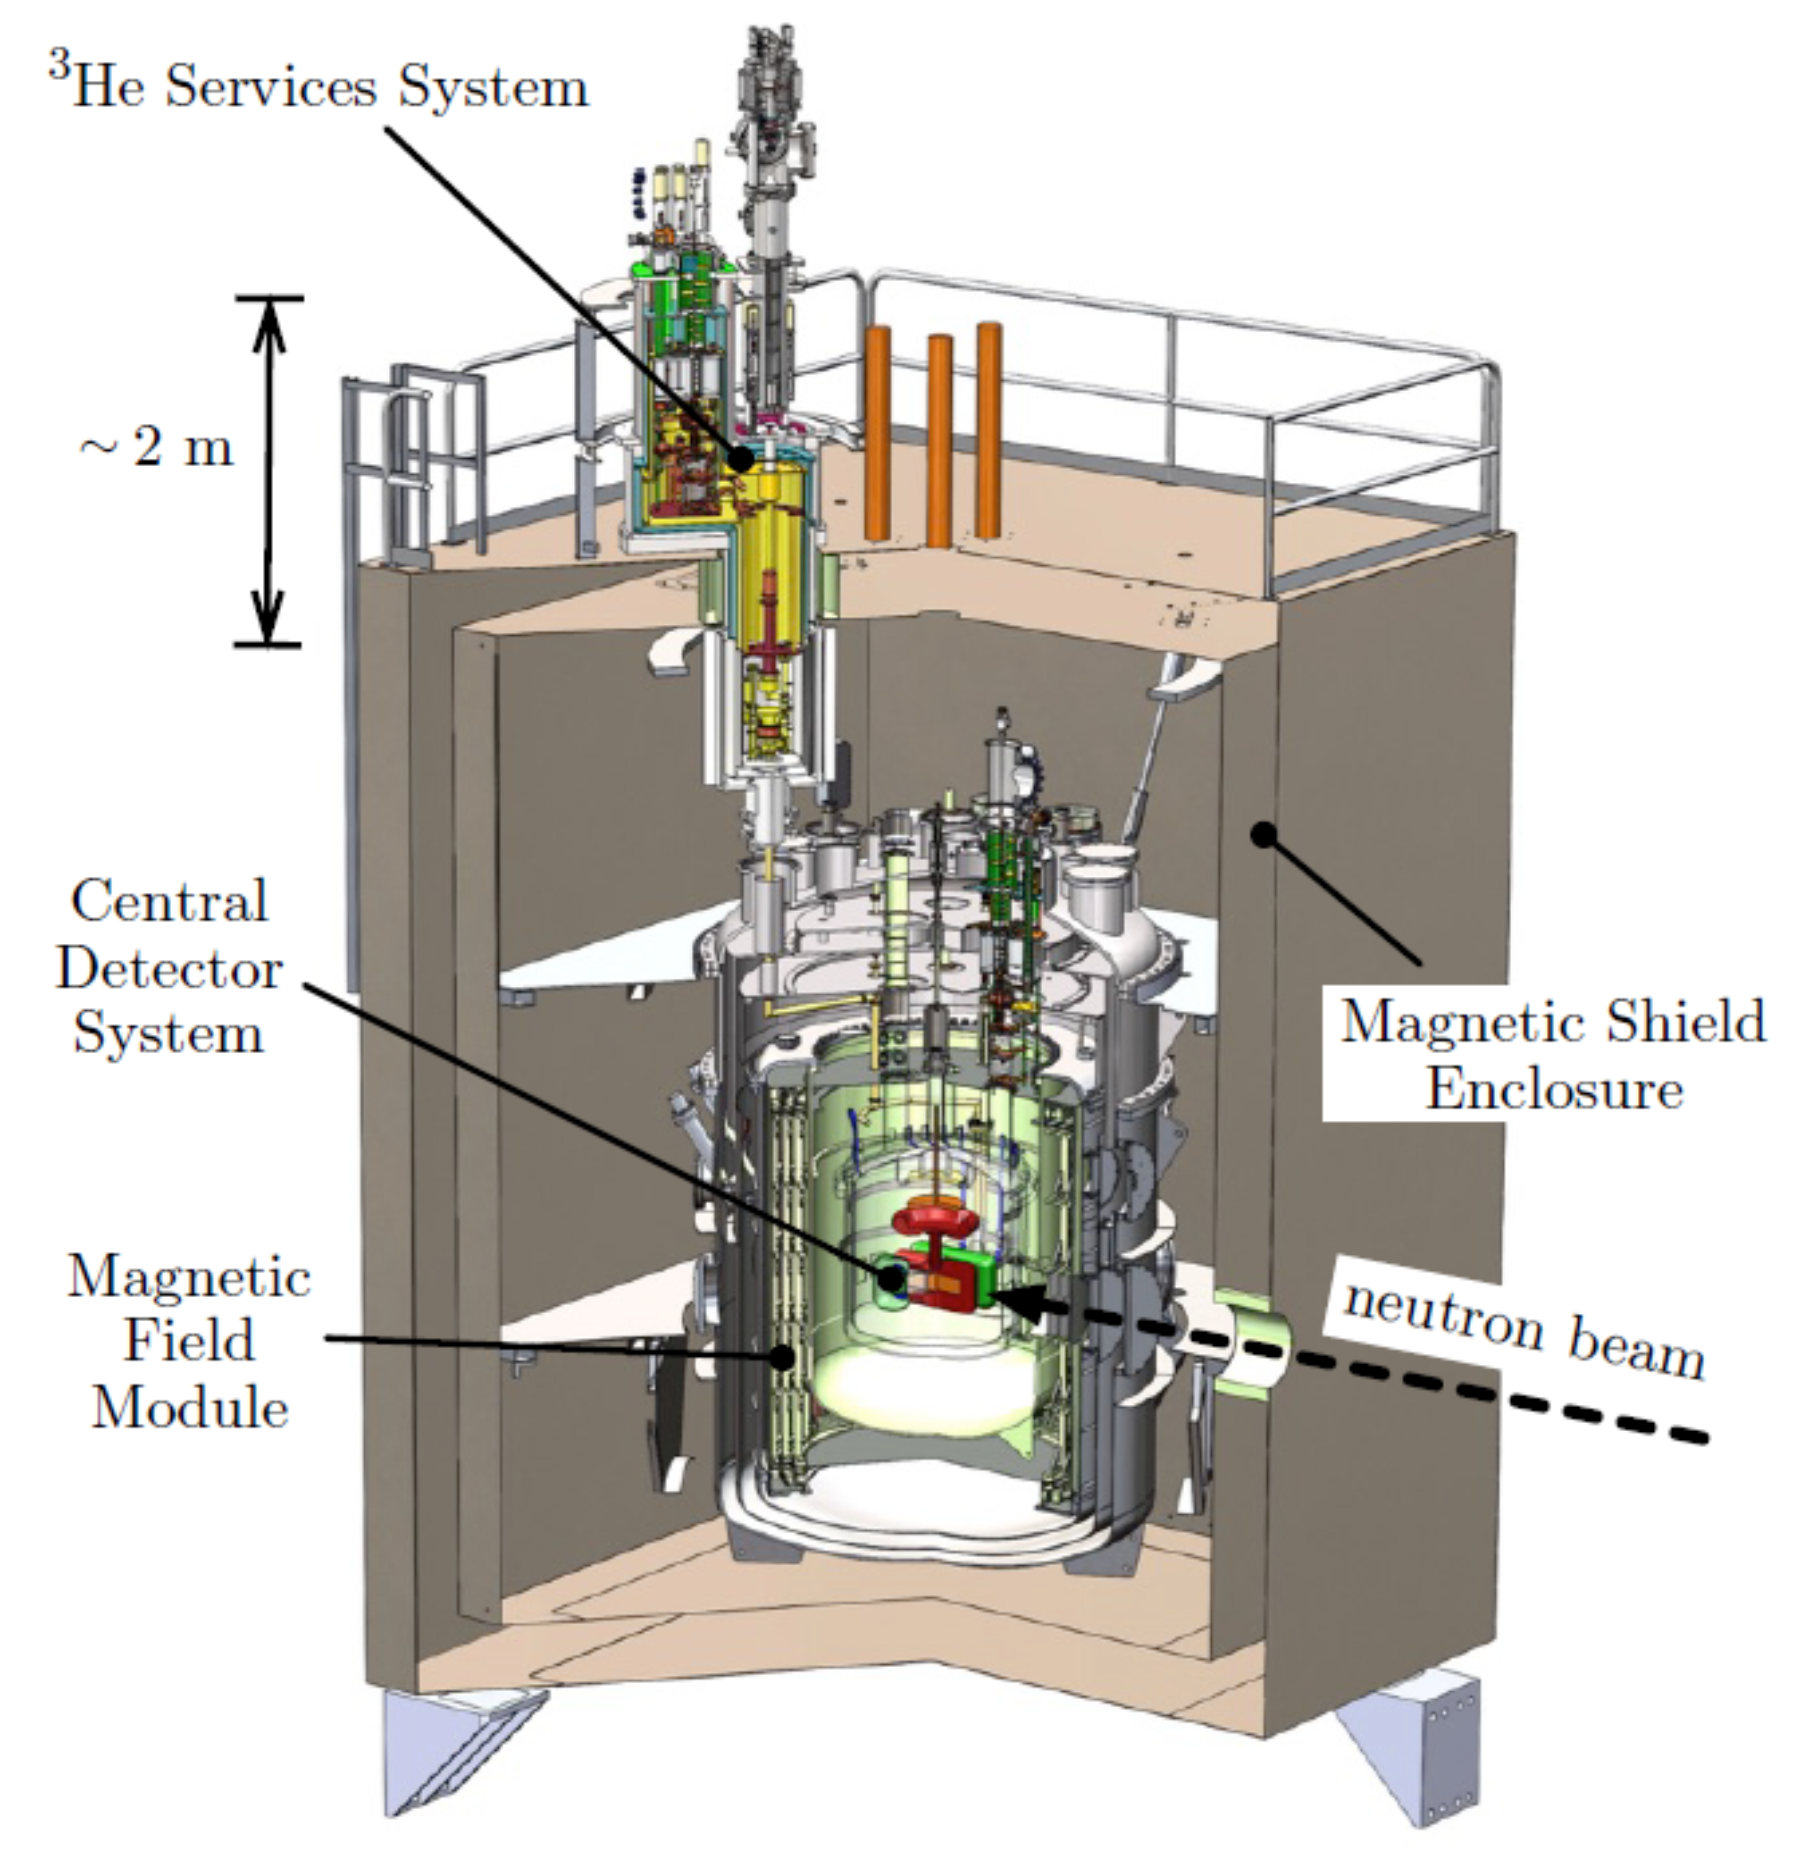
\includegraphics[width=1\textwidth]{nEDM_SNS_experiment.png}
    \caption[Schematic overview of the key nEDM@SNS experimental apparatus.]{Schematic overview of the key nEDM@SNS experimental apparatus. Figure taken from \cite{Ahmed2019}.}
    \label{fig:key_nEDM@SNS}
\end{figure}
\clearpage}

\subsection{Central Detector system}

The Central Detector System (CDS), shown in greater detail in \cref{fig:CDS}. The CDS volume is made of fiberglass composite which will be filled 1600 L of superfluid helium and cooled to 0.4~K with a non-magnetic dilution refrigerator (DR). The purpose of the CDS is to harbor the two measurement cells, the high voltage electrode system, SQUID magnetometers array, and the  scintillation light collection fibers. The entire CDS volume along with its inner components is made of non-magnetic materials to prevent field gradients and non-electrically conductive materials to prevent the thermal ringing noise in the SQUIDS as well as eddy current heating from the RF magnetic fields. 

\afterpage{
\begin{figure}
    \centering
    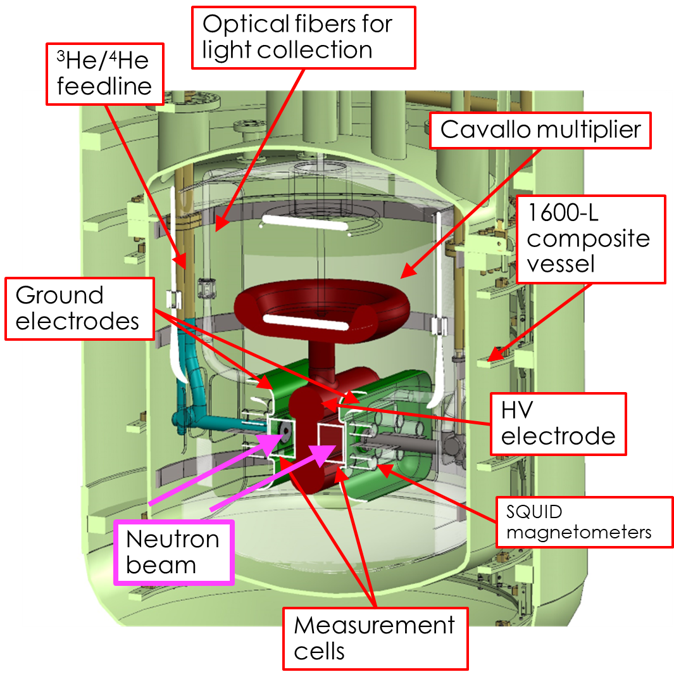
\includegraphics[width=1\textwidth]{figures/chapter2-figs/CDS_detail.png}
    \caption{A detailed view of the Central Detector System (CDS). Figure courtesy of Takeyasu Ito of the nEDM@SNS collaboration.}
    \label{fig:CDS}
\end{figure}
\clearpage}

As stated earlier, the measurement cells will be composed of acrylic PMMA with inner walls coated in highly pure deuterated polystyrene (dPS) with embedded deuterated tetraphenyl butadiene (dTPB). The cell will be 40 cm long, 7.5 cm wide and 10 cm tall with a wall thickness of 1.2 cm. The cell materials are deuterated to allow for UCN production as well as provide a long UCN storage time by preventing upscattering of UCNs. The purpose of dTPB is to wavelength shift the scintillation light for collection and extraction by the light fibers guides \cite{McKinsey1997}. A deuterated plastic valve in between the two cells will allow (un)loading of (de)polarized $^3$He into the measurement cells. 

The high voltage electrodes will be made of PMMA with electrically conductive coating. The desired 75 kV/cm electric field corresponds to a potential of 630 kV of the longitudinal area of the cell. A cryogenic high voltage amplification system, called the Cavallo multiplier, will be used to provide the large electric potential \cite{Ahmed2019}. The operating principle of electrostatic charge transfer based on the relative capacitance of each of the electrodes in the amplification process is shown in \cref{fig:Cavallo}.

\afterpage{
\begin{figure}
    \centering
    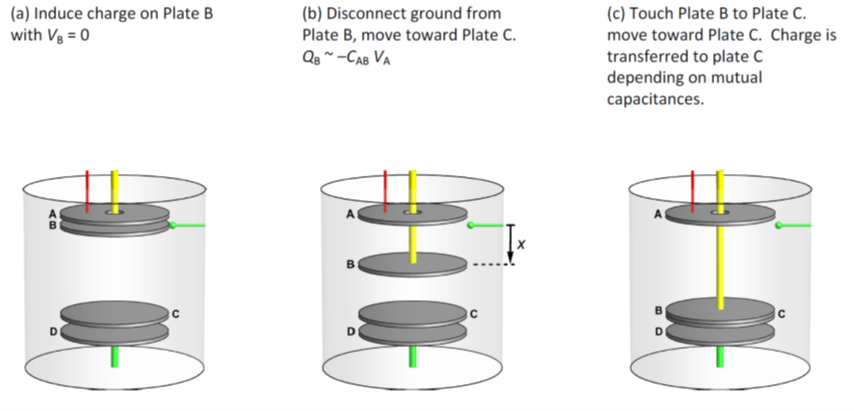
\includegraphics[width=1\textwidth]{figures/chapter2-figs/Cavallo_schematic.png}
    \caption[A schematic showing the operating principle of Cavallo high voltage amplification system design for the nEDM@SNS experiement.]{A schematic showing the operating principle of Cavallo high voltage amplification system design for the nEDM@SNS experiement. Figure taken from \cite{Ahmed2019}.}
    \label{fig:Cavallo}
\end{figure}
\clearpage}

\subsection{Polarized ${^3}$He System}

The polarized $^3$He system, as shown in \cref{fig:3He_sys}, will be located atop the CDS as shown in \cref{fig:key_nEDM@SNS}. The polarized $^3$He system has three functions for the operation of the nEDM@SNS experiment: (i) polarize the $^3$He, (ii) inject the polarized $^3$He into the measurement cells and (iii) remove the depolarized $^3$He from the measurement cells \cite{Ahmed2019}.

$^3$He will be polarized using an atomic beam source (ABS) \cite{Esler2007, Eckel2012}. This cryocooled $^3$He source uses inhomogeneous magnetic fields from a quadrupole magnet to filter out one spin state, polarizing the $^3$He atoms \cite{Ahmed2019}. The polarized $^3$He will be injected into the measurement cell by applying temperature gradients which induce phonons (‘heat flush’) that will carry the polarized $^3$He \cite{Baym2015}. This polarization will be adiabatically maintained via spin transport magnetic fields. After the spin precession measurement is finished, the depolarized $^3$He will be removed via the heat flush technique into a separate volume, to be discarded. 

\afterpage{
\begin{figure}
    \centering
    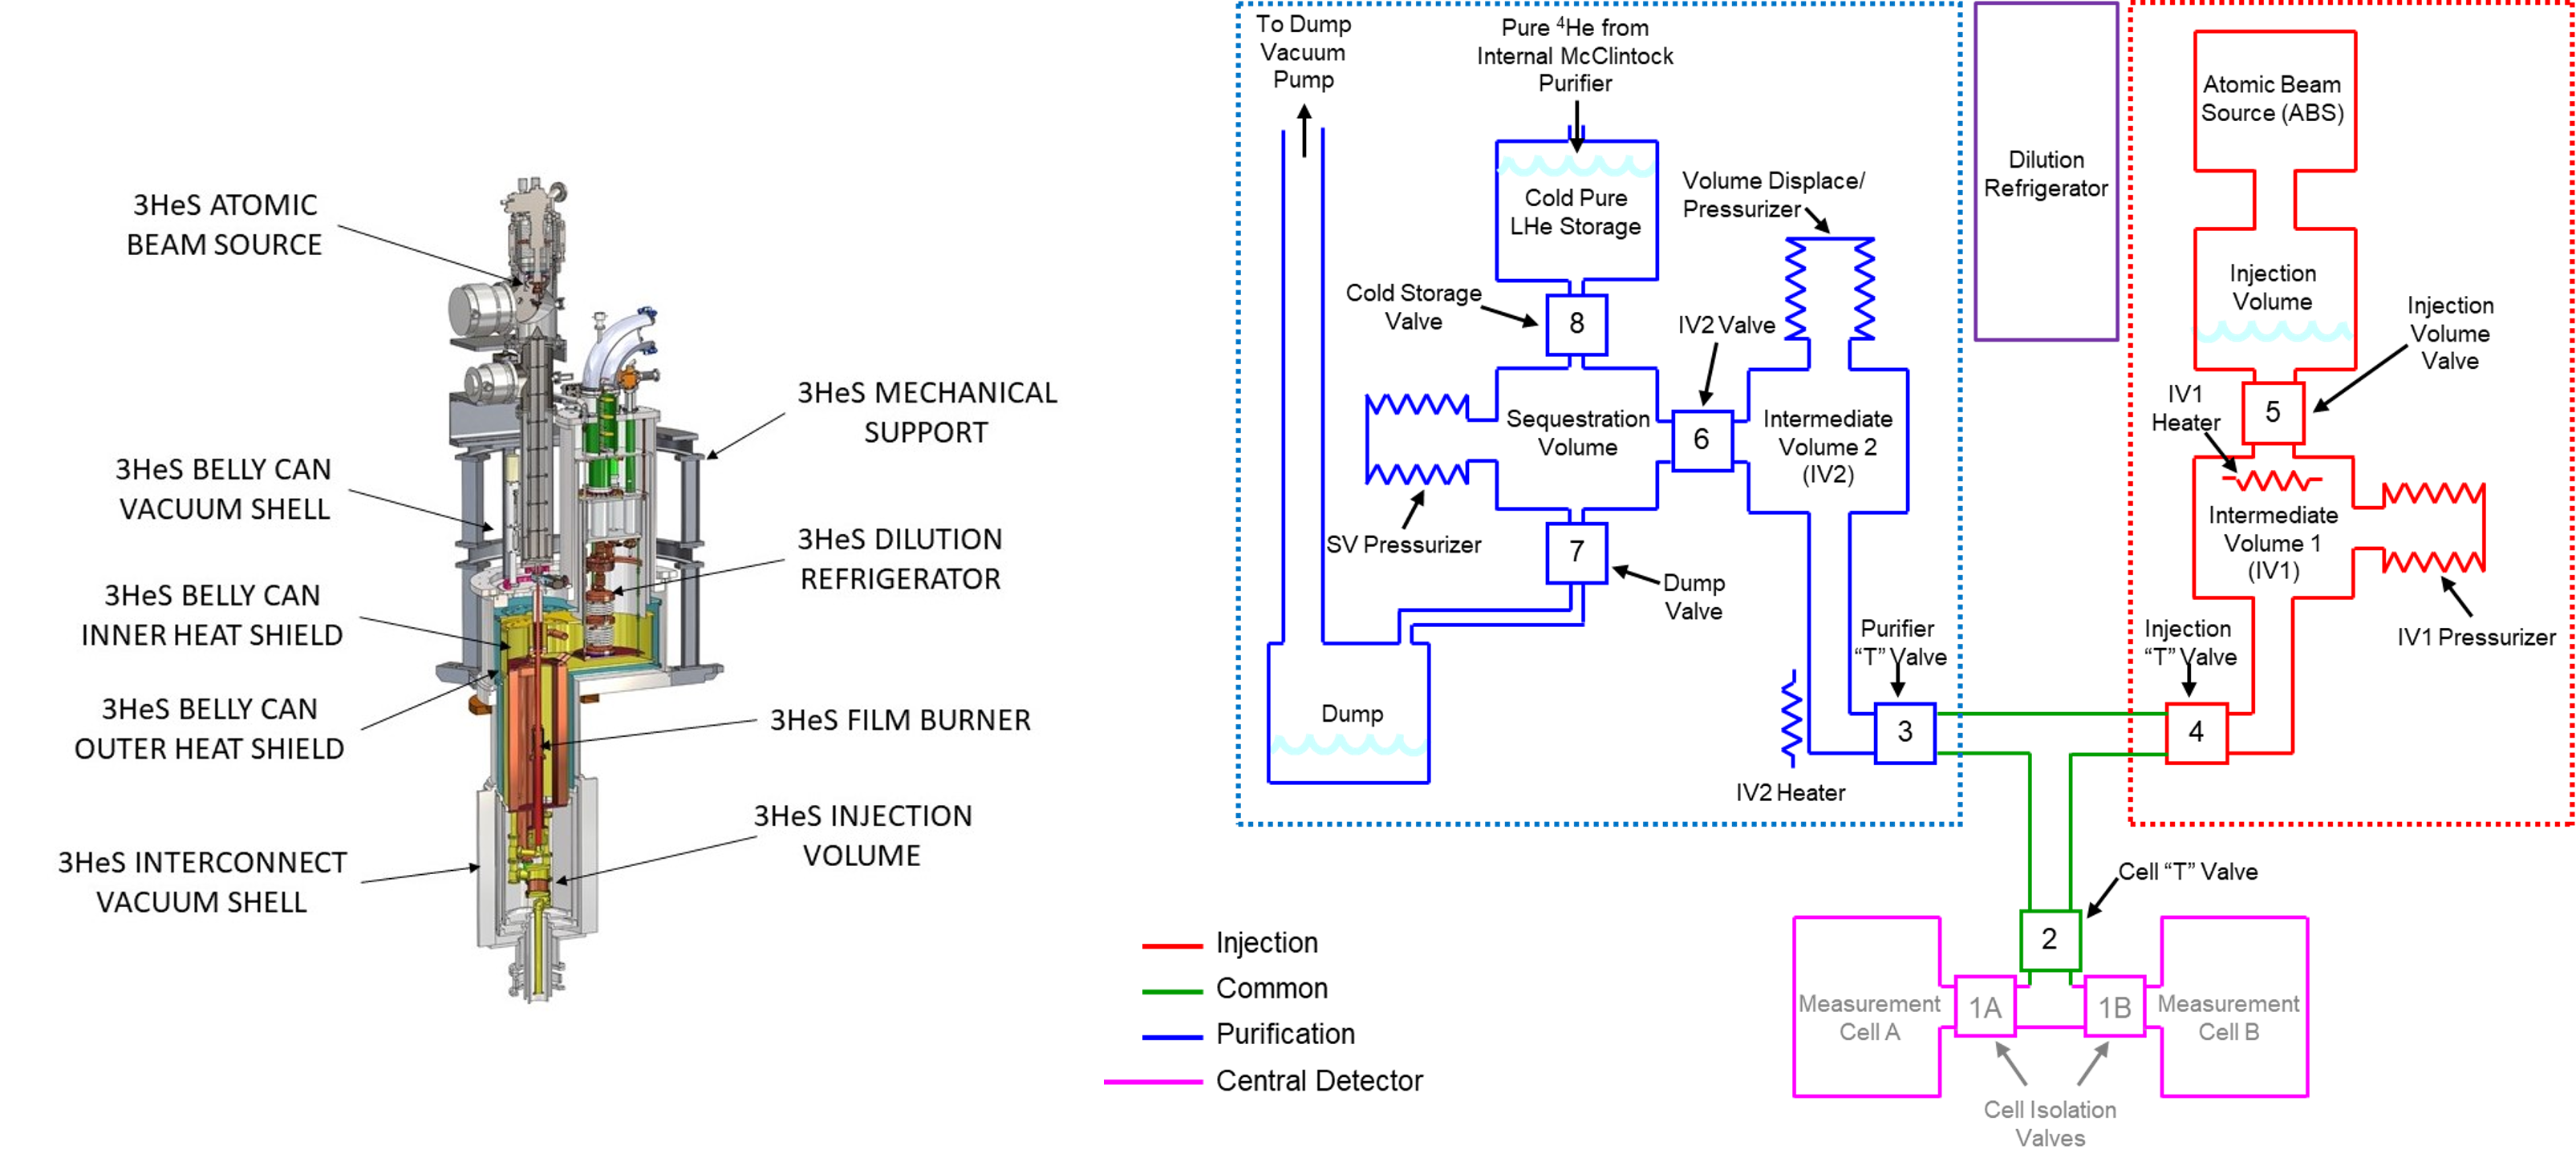
\includegraphics[width=1\textwidth]{figures/chapter2-figs/3He_detail.png}
    \caption[Overall schematic of the polarized $^3$He subsystem.]{Overall schematic of the polarized $^3$He subsystem. Figure on the left is taken from \cite{Ahmed2019} and figure on the right is courtesy of Steve Williamson of the nEDM@SNS collaboration.}
    \label{fig:3He_sys}
\end{figure}
\clearpage}

\subsection{Magnetic Field Module System}

The Magnetic Field Module (MFM), which surrounds the CDS, is responsible for providing all of the magnetic fields relevant for the spin precession measurements as well as the appropriate magnetic shielding. A schematic of this system is shown in \cref{fig:MFM}. 

\afterpage{
\begin{figure}
    \centering
    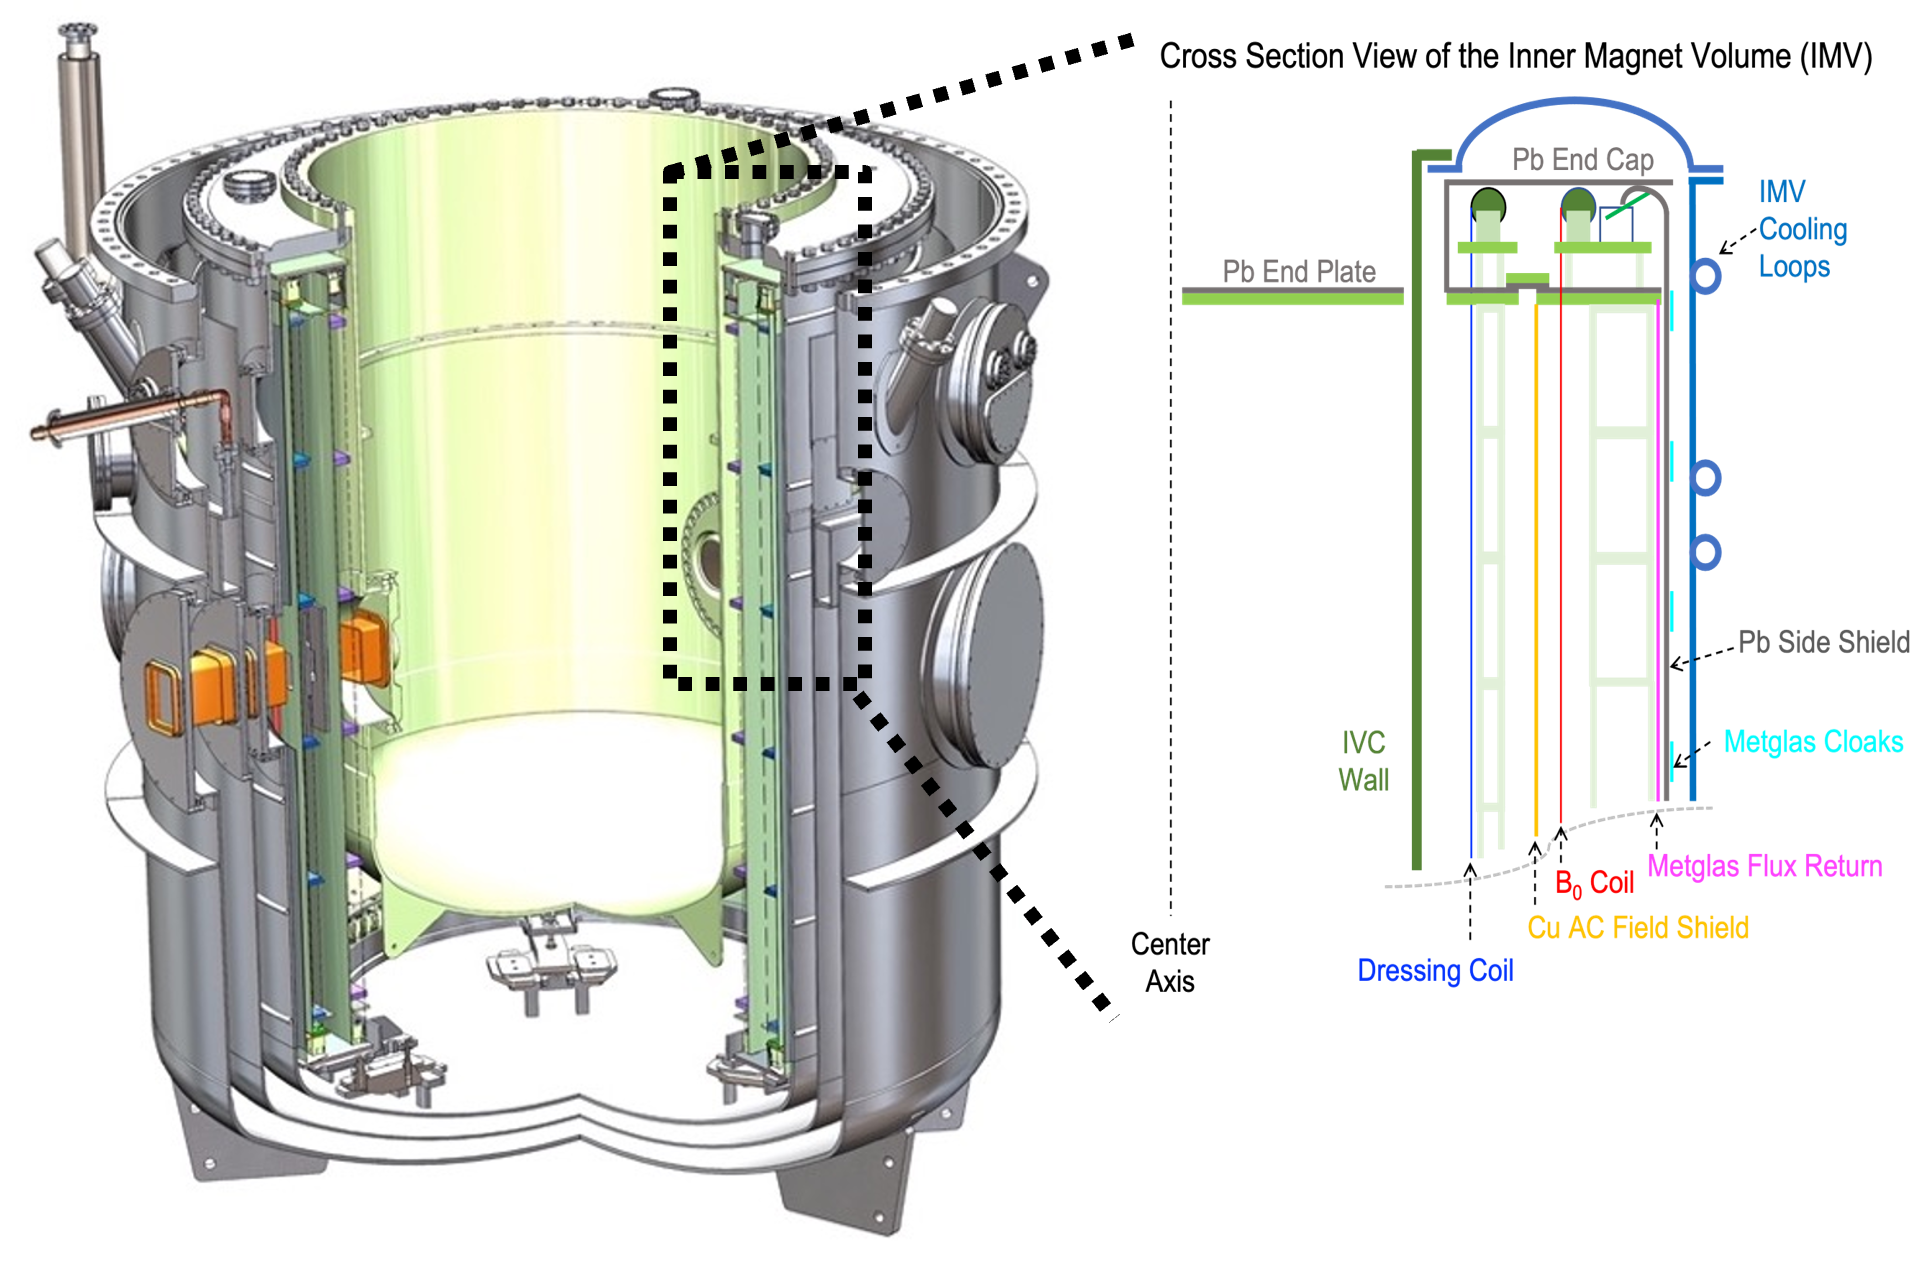
\includegraphics[width=1\textwidth]{figures/chapter2-figs/MFM.png}
    \caption[Overall schematic of the Magnetic Field Module system.]{Overall schematic of the Magnetic Field Module system. Figure taken from \cite{Ahmed2019}.}
    \label{fig:MFM}
\end{figure}
\clearpage}

Going outwards from the center, the vertical concentric cylindrical components of the MFM are: the spin dressing cos$\theta$ coil to provide RF fields, transverse to $B_0$ magnetic field, for the $\pi$/2 rotation and spin dressing, a thin conductor eddy current shield to reduce heating from the spin dressing field, a cos$\theta$ $B_0$ coil to provide the uniform 30 mG field in the horizontal direction, a ferromagnetic shield made of high permeability material, Metglas, to provide a flux return for the $B_0$ field and improving the $B_0$ uniformity, and lastly a superconducting Pb magnetic shield for eliminating time varying drifts in the magnetic fields. Two Pb layers cap the top and bottom ends of the MFM with the return loops of the $B_0$ coil on the outside to mimic the $B_0$ coil if it were of infinite length and further improve the field uniformity. The expected magnetic field gradients based on the design are less than $1\times 10^{-7}$ G cm$^{-1}$. A schematic of the fields produced by the MFM is shown in \cref{fig:MFM_Bfields}. A cylindrical array of fluxgate magnetometers will be located between the MFM and the CDS \cite{Ahmed2019} to allow for coarse tuning of magnetic field gradients.

\afterpage{
\begin{figure}
    \centering
    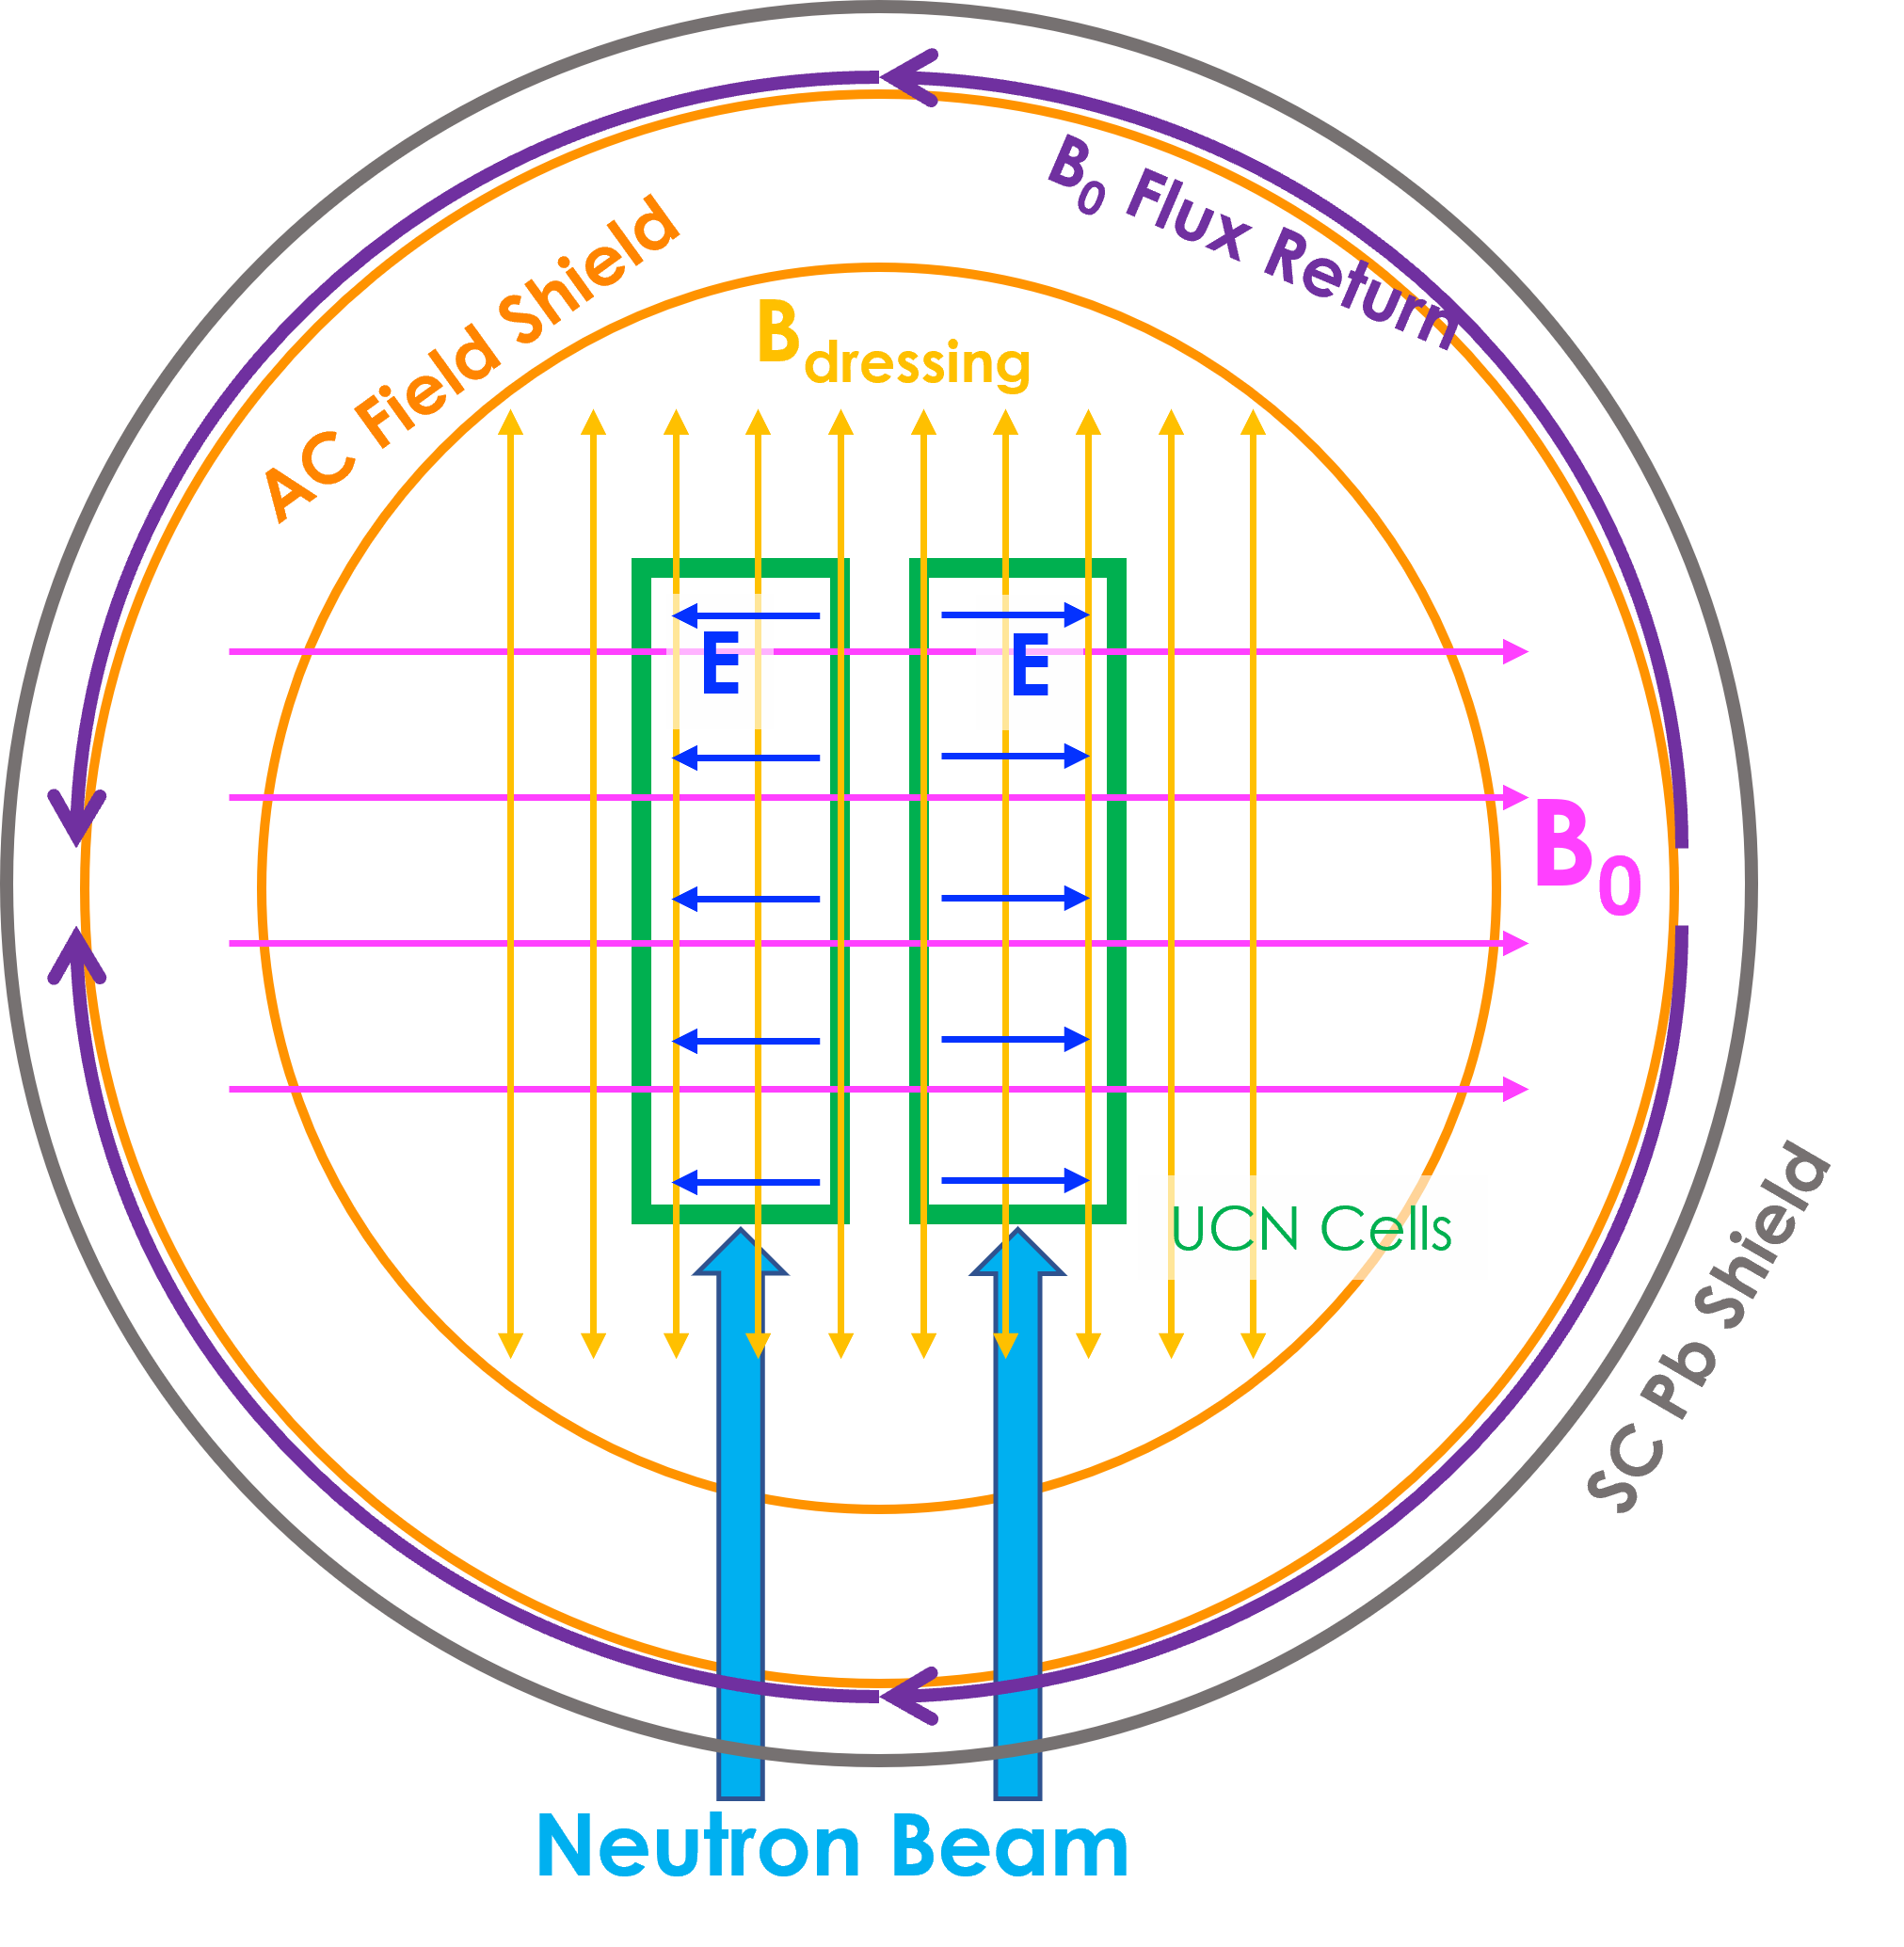
\includegraphics[width=1\textwidth]{figures/chapter2-figs/MFM_Bfields.png}
    \caption{A top down cross-sectional view of the main magnetic field generating components of the Magnetic Field Module. Figure courtesy of Wanchun Wei of the nEDM@SNS collaboration.}
    \label{fig:MFM_Bfields}
\end{figure}
\clearpage}

The next set of the outer layers form the cryostat of the MFM, which consist of the inner magnet volume (IMV) which operates at 4 K, the liquid nitrogen shield (LN$_2$ shield), which operates at 77 K and reduces radiative heat load on the IMV and lastly, the outer vacuum chamber (OVC), which forms the vacuum boundary as well as prevents conductive warming of the low-temperature components.

The entire nEDM@SNS apparatus (CDS, MFM and polarized $^3$He system) will reside inside a large 4 m by 4m wide and 6 m tall multi-layered ferromagnetic Magnetic Shield Enclosure (MSE) made of high permeability material called mu-metal. This MSE is shown in \cref{fig:key_nEDM@SNS}. The purpose of the MSE is to provide a less than $1\times 10^{-5}$ G m$^{-1}$ field gradient and a high shielding factor for external RF fields at its center, where the measurement cells will reside. Outside the MSE will be coil pairs along the orthogonal axes of the MSE to cancel out the earth’s magnetic field.

The major components of the apparatus described exist and are expected to undergo full assembly in the upcoming years, with the first nEDM measurement data expected to begin in 2029. As part of this development effort, neutron polarization and transmission measurements need to be performed to check for the neutron intensity and polarization loss from the MFM. These measurements are the main topic of this dissertation and the associated neutron polarimetry is described in the succeeding chapters.
    \chapter{Polarized $^{3}$He for Neutron Spin Analysis}
\label{ch:polHe}

\ifpdf
    \graphicspath{{Chapter2/Figs/Raster/}{Chapter2/Figs/PDF/}{Chapter2/Figs/}}
\else
    \graphicspath{{Chapter2/Figs/Vector/}{Chapter2/Figs/}}
\fi

This chapter describes the in situ (at the experiment location) $^3$He SEOP polarization setup used for the neutron polarization and transmission measurements at the SNS Beamline 13A. First, the methodology to polarize $^{3}$He is described, then the design of the in situ system along with the results from proof of demonstration are shown and discussed.

\section{Polarized $^{3}$He}

Targets of gaseous spin polarized $^3$He nuclei are widely used in nuclear physics as polarized “free neutrons” for electron scattering experiments and as spin filters/analyzers of polarized neutron beams due to the large spin dependent absorption cross section of neutrons by $^3$He \cite{Gentile2017}. Convenience of long polarization relaxation times ($\sim 10^2$ hours) due to the noble gas chemical inertness, absence of an electric quadrupole moment and the presence of a large magnetic moment make $^3$He attractive for precision measurements. This utility is enabled by methods used to hyperpolarize $^3$He atoms. 

It is not possible to directly polarize the $^3$He 1s$^2$-1s2p transition since the hyperfine splitting in 1s2p state is very small, resulting in mixing of the hyperfine levels of the excited state, not to mention, the lack of 59nm (extreme UV) laser technology \footnote{Technically, one can use a Stern-Gerlach filter or the Lamb shift transitions in the small Zeeman splitting of the 2s[F=1/2] states in $^3$He to polarize $^3$He \cite{Schieck2011}.} \cite{Schieck2011}. Thus spin exchange (SEOP) and metastability exchange (MEOP) optical pumping methods involving indirect transfer of angular momentum are used \cite{Gentile2017}. In SEOP, alkali atoms at $\sim$bar pressure are polarized via optical pumping of their electronic structure \cite{Walker1997}. Transfer of angular momentum from alkali to He occurs via slow and weak Hyperfine interactions \cite{Walker1997}. In MEOP, metastable $^3$He atoms are created via optical pumping and are rapidly polarized via weak Hyperfine mixing \cite{Batz2011}. The polarized metastable $^3$He atoms are transferred to the polarized ground state $^3$He via exchange collisions \cite{Batz2011}. This section gives a brief overview of the two optical pumping methods to provide context for this thesis. A more comprehensive overview can be found in \cite{Gentile2017}.

\subsection{Spin Exchange Optical Pumping}

%In SEOP, alkali atoms are polarized via optical pumping of their electronic structure. Transfer of angular momentum from alkali to $^3$He transpires via slow and weak Hyperfine interactions \cite{Bouchiat1960,Walker1997}. 

The first demonstration of SEOP on $^3$He was done by \cite{Bouchiat1960} in 1960. With the advancement in laser technology, \cite{Chupp1987} used laser based SEOP to develop high density polarized $^3$He for discriminating neutron polarization. Even today, the laser based SEOP is the most widely used technique to perform SEOP.

Glass cells filled with 0.1 to 10 bar\footnote{All pressures listed in this section are at standard temperatures unless otherwise stated.} pressure of ultra-high purity (99.999\%) $^3$He gas along with $\sim$100mg of Rubidium and Potassium alkali metal mixture are used for confining and polarizing $^3$He. The cells are heated to 190~\degree C to 210~\degree C to vaporize the alkali mixture to achieve a density of around $10^{14}-10^{15}$ cm$^{-3}$. The entire cell is illuminated with circularly polarized infrared light using a diode laser. The laser output is typically set to 50 W to 100 W power and 795 nm or 770 nm wavelength, which correspond to the D1 transition lines of Rb and K, respectively, with a linewidth of about 0.2 nm \cite{Gentile2017, Ben-AmarBaranga1998, Chen2014}. The alkali density in cells is low enough that the spectral width of the laser is enough to cover the atomic line width broadening from relatively high pressure nature of the cell \cite{Romalis1997, Kluttz2013}. Even though a high degree of circular polarization can be attained with commercial polarizing wave plates \cite{Bhaskar1979, Chann2002}. A small amount of nitrogen gas is also added to quench the radiative decay of the excited alkali atoms \cite{Walker1997, Lancor2010}.

The build up of alkali polarization is determined by a large alkali polarization optical pumping rate as compared to the alkali polarization relaxation rate \cite{Gentile2017}. The alkali spin-relaxation times are on the order of a few ms, whereas the alkali optical pumping times are much shorter, typically $\lesssim$ ms, hence high alkali polarization is established relatively quickly \cite{Chen2011}. These short optical pumping times are possible because of the use of laser based optical pumping as well as keeping the cell at a high temperature to vaporize the optically thick alkali mixture \cite{Gentile2017, Chen2011, Babcock2016}. The alkali spin relaxation is primarily caused by alkali-alkali collisions and alkali-$^3$He collisions \cite{Ben-AmarBaranga1998}. This relaxation due to collisions is highly dependent upon the pressure of $^3$He gas and amount of alkali mixture used during formation of the $^3$He cell \cite{Ben-AmarBaranga1998}. A hybrid mixture of K and Rb alkali atoms is used due to their high spin exchange efficiency and low spin relaxation rates \cite{Babcock2003, Chen2007}.

Similarly, the build up of $^3$He polarization is determined by a large alkali-$^3$He spin-exchange rate as compared to the $^3$He nuclear spin relaxation \cite{Gentile2017}. The alkali-$^3$He spin exchange time is typically on the order of 10 hours, hence, it takes a day(s) to approach the maximum attainable $^3$He polarization \cite{Chen2011, Gentile2017}. Due to these slow polarization times, it is critical to have long $^3$He polarization relaxation times for a cell in order to maximize its use. GE180, a type of Aluminosilicate glass, which has low $^3$He permeability, is boron free and corrosion resistant, is widely used for neutron based experiments \cite{Newbury1993, Chen2014, Heil1995}. Polarized $^3$He cells at room temperature have shown relaxation times on the order of 100 hours  \cite{Chen2011}. This indicates that relaxation due to glass cell wall has a minor contribution towards limiting the attainable $^3$He polarization. However, relaxation from temperature effects has been found to restrict the $^3$He polarization \cite{Babcock2006}. These main limiting effects will be discussed later in this chapter.

In a typical SEOP apparatus, an oven is used to heat the glass cell filled with of alkali mixture and $^3$He \cite{Tong2010, Babcock2016}, a magnetic field coil to provide uniform holding magnetic field, a high-power laser with narrow spectral width \cite{Babcock2005, Chen2014, Liu2015} and laser optics for generating circularly polarized light and steering/focusing the laser beam. $^3$He polarization is monitored and controlled using nuclear magnetic resonance (NMR) techniques as well as alkali spectroscopy \cite{Romalis1998}.


\subsection{Metastability Exchange Optical Pumping}

In MEOP, $^3$He is polarized via optical pumping and hyperfine interactions of metastable $^3$He atoms followed by rapid transitions to the ground state via metastable state to ground state exchange collisions \cite{Colegrove1963, Batz2011}.  MEOP is usually performed on $^3$He cells with pressures on the order of $\sim$mbar. External electrodes are used to produce a RF discharge to make metastable atoms on the order of $10^{10}$ cm$^{-3}$ \cite{Colegrove1963, Batz2011, Gentile2017}. Ionization of impurities can lead to destruction of metastability, so ultra-high purity gases and clean glass cells are used. The low density of $^3$He means low density of metastable states, hence, larger cells are used to absorb the optical pumping light to overcome the optically thin nature and  yield larger quantities of polarized $^3$He. Optical pumping is performed via $\sim$10W lasers at the 1083nm wavelength with spectral linewidth of 15 cm \cite{Colegrove1963, Batz2011, Gentile2017}. This linewidth is much wider than the Doppler-broadened atomic absorption \cite{Colegrove1963, Batz2011, Gentile2017}. The polarization of the $^3$He ground state and metastable $^3$He states are strongly coupled due to the hyperfine interactions \cite{Gentile2017}, and subsequently evolve on the timescale of seconds \cite{Gentile1993}. The $^3$He ground-state relaxation is dependent on the strength of the RF discharges, where strong discharges produce higher densities of metastable states and thus, higher polarization, however, at the expense of large metastability induced relaxations \cite{Batz2011, Gentile2017}. 

The apparatus used to perform MEOP consists of RF discharge electrodes wrapped around the $^3$He cell. The cells resides in a homogeneous magnetic field, which is provided by a large set of coils. The cell is illuminated with a laser outputting circularly polarized IR light \cite{Andersen2005}. During optical pumping, compressors are also used to maintain the $^3$He polarization \cite{Andersen2005}. After compression, NMR is used to monitor/manipulate the $^3$He polarization \cite{Romalis1998}.

\subsection{Comparison of SEOP and MEOP}

Although both SEOP and MEOP can be used to produce polarized $^3$He, the application has to be considered in order to select the appropriate method. The benefit of SEOP is enabling of means to polarize from 0.3 bars to 10 bars pressure $^3$He cells \cite{Gentile2017}. By contrast, MEOP is best deployed for $\sim$1 mbar pressures, requiring further gas compression to preserve the polarization \cite{Gentile2017}. The advantage of MEOP is the ability to polarize $^3$He at timescales faster (typically seconds) than most SEOP (typically hours) \cite{Gentile2017}.  In terms of operations, SEOP can be done in compact setups without the need for supervision during the hours long build up towards polarization \cite{Jiang2013}, while MEOP requires large laboratory space to accommodate the bulky setup as well as live supervision to operate the gas compression, albeit for short times \cite{Batz2011}. For neutron applications, such as the experiment described in this thesis, a 0.8bar $^3$He cell was used in a compact in situ apparatus, therefore SEOP was the suitable method. SEOP has also been the preferred choice for other $^3$He cells/neutron spin fliters used at Oak Ridge National Laboratory, therefore, the presence of technical expertise and pre-existing equipment was beneficial to the work described in this thesis. 

\section{Theory of Spin Exchange Optical Pumping}

\subsection{Optical Pumping}

As stated earlier in this chapter, the SEOP process facilitates the polarization of $^3$He by polarized alkali atoms, therefore, it is necessary to optically pump and polarize the alkali with high efficiency. This optical pumping is performed using monochromatic high powered lasers with sharp spectral widths to initiate the hyperfine atomic transitions of the alkali atoms. This section describes the physics of alkali optical pumping, the causes of alkali spin relaxation as well the circularly polarized light dependent effects on the efficiency of optical pumping. A detailed explanation of the optical pumping mechanism can be found in \cite{Gentile2017, Happer1987, Walker2011}. The SEOP mechanism described in this section is adopted from the terminology and nomenclature in \cite{Gentile2017}.

\afterpage{
\begin{figure}
    \centering
    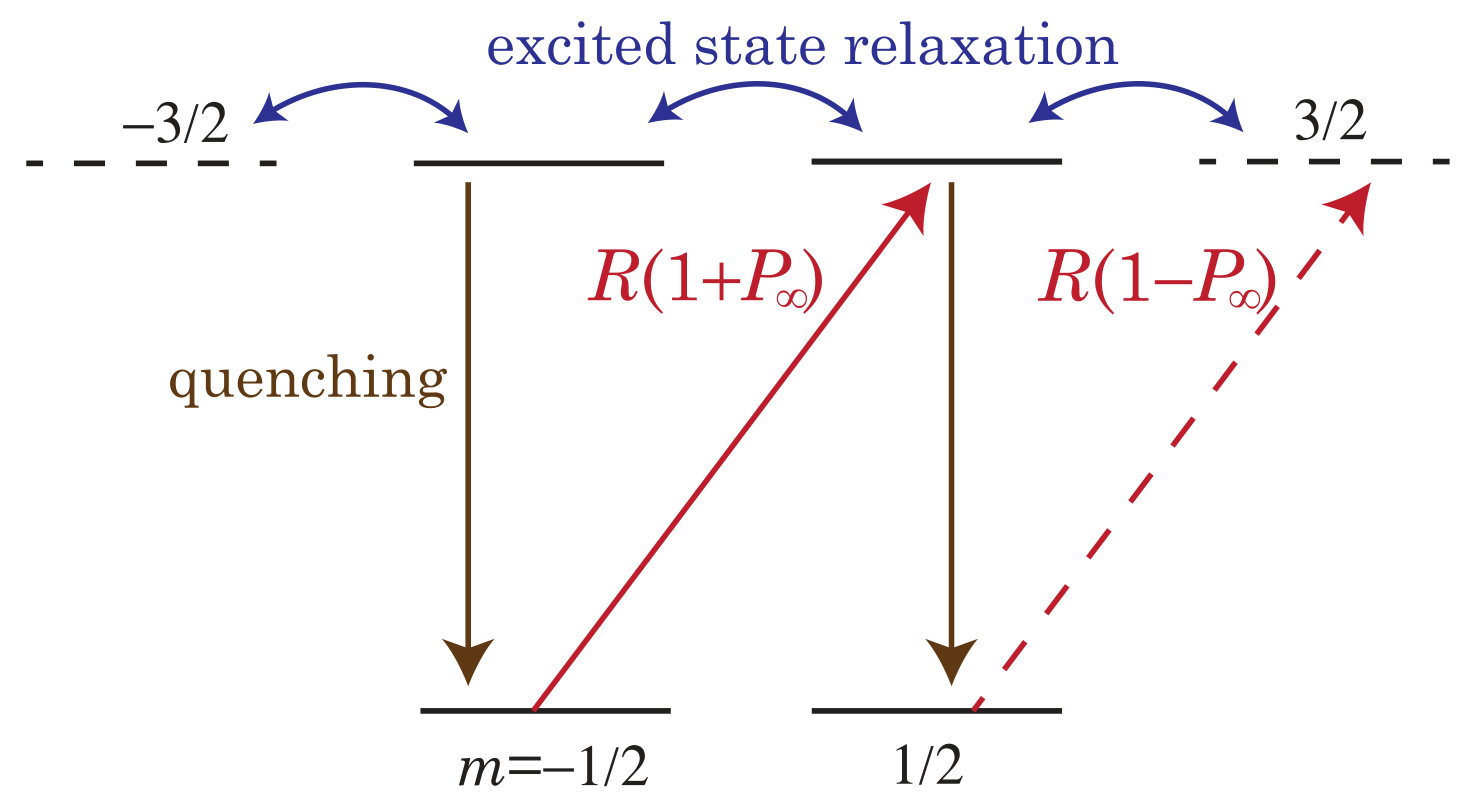
\includegraphics[width=\textwidth]{figures/chapter3-figs/OPalkalistates.png}
    \caption[Hyperfine atomic levels involved in the the optical pumping via light of the alkali $S_{1/2}$ to $P_{1/2}$ D1 resonance in the presence of $^3$He.]
    {Hyperfine atomic levels involved in the the optical pumping of the alkali $S_{1/2}$ to $P_{1/2}$ D1 line in the presence of $^3$He. The $^3$He atoms mix the P-levels of the alkali, modifying the ground state to the excited state selection rules. Alkali in the $m_S= \pm \frac{1}{2}$  ground-state Zeeman sublevels absorb light with $1 \mp P_{\infty}$, probability. Once the alkali transitions to the excited state, spin relaxing collisions can occur. N$_2$ gas is used to quench any alkali radiative and al de-excitations and relaxes the alkali to the ground-state Zeeman sublevels. The alkali, over time, accumulates in the $m_S=\frac{1}{2}$ Zeeman sublevel, acquiring a steady-state hyperfine spin polarization of $P_{\infty}$ assuming that spin relaxation in the alkali ground-state is absent. Figure taken from \cite{Gentile2017}.}
    \label{fig:opticalpumping}
\end{figure}
\clearpage}

A more detailed description of the alkali atomic spectrum especially the D lines of Rb and K can be found in \cite{Steck2023Rb85, Steck2023Rb87, Tiecke2019}. \Cref{fig:opticalpumping} shows the relevant hyperfine levels at play during the optical pumping of alkali atoms. It illustrates the optical pumping mechanism from circularly polarized ($\sigma_+$) light absorption tuned to the ground state $S_{\frac{1}{2}}$ to the excited state $P_{\frac{1}{2}}$ “D1” resonance line of the alkali. The figure also shows the presence of mixing of the $P_{\frac{1}{2}}$ and $P_{\frac{3}{2}}$ Zeeman sublevels due to collisions with $^3$He atoms indicated by the dashed lines. 

As illustrated in \cref{fig:opticalpumping}, the D1 line transition probability, $P_{\infty}$, for alkali atoms in the $m_S=-\frac{1}{2}$ Zeeman sublevel transitioning to the the $m_P=\frac{1}{2}$ level is $1+P_{\infty}$. This transition probability much large than the transition probability of $1-P_{\infty}$ for the alkali in the $m_S=\frac{1}{2}$ Zeeman sublevel \cite{Gentile2017, Happer1987, Lancor2010}. This selective transition is possible due to the mixing from the weak hyperfine interactions under the presence of $^3$He \cite{Gentile2017, Happer1987}. Therefore, the alkali atoms in the $m_S=-\frac{1}{2}$ ground state get preferentially excited to $m_P=\frac{1}{2}$ excited state. The excited alkali atoms undergo relaxation due to collisions with the $^3$He gas and an additional quenching gas, N$_2$. This randomizes the excited alkali atom population among the mixed $P_{\frac{1}{2}}$ and the $P_{\frac{3}{2}}$ Zeeman sublevels. Then, there is resonant transfer of the excited alkali P-state energy to vibrational states of N$_2$. This de-excites the alkali atoms back to the $S_{\frac{1}{2}}$ ground state level. The fraction of alkali atoms that de-excite to the $m_S=\frac{1}{2}$ state do not absorb the polarized light, due to selection rules. While the fraction that de-excite to $m_S=-\frac{1}{2}$ get excited back to P-states and relax until all alkali atoms populate the $m_S=\frac{1}{2}$ state. The process continues until a steady-state polarized alkali population builds up, $P_{\infty}$ \cite{Lancor2010}. N$_2$ plays a key role in this process by quenching the excited alkali atoms to prevent radiative de-excitations \cite{Lancor2010}. The mechanism described is valid for high alkali density cells \cite{Gentile2017, Walker1997, Happer1987}. However, for low alkali density cells, rapid electronic de-excitations cause nuclear spin relaxation via hyperfine couplings, reducing the optical pumping efficiency \cite{Lancor2010}.

The spin-exchange collisions among the alkali-metal atoms themselves are responsible for maintaining the collective angular momentum \cite{Happer1972, Appelt1998}. These collisions conserve the total angular momentum ($F_{A}=I_{A}+S_{A}$) and in combination with the alkali hyperfine coupling, establish a thermal spin equilibrium with the total angular momentum states ($F, m_{F}$) as $\rho \propto \exp \left({\frac{ m_{F}}{k_BT}} \right) $ \cite{Happer1972, Appelt1998}, where $k_B$ is the Boltzmann constant and $T$ is temperature. The alkali-metal electron spin polarization can be defined with this spin-temperature parameter as $P_A = \tanh{\frac{1}{2k_BT}}$. In the mechanism described so far, the alkali nuclear spins have neglected. However, since SEOP $^3$He cells are pumped under the application of low magnetic fields, the total alkali hyperfine structure (with a non-zero alkali nuclear spin) and the total angular momentum states ($F, m_{F}$) with ($2F+1$) multiplicity have to be considered. Pressure broadening of the D1 line leaves the total angular momentum states $m_{F}$ unresolved, therefore, all $m_{F}$ states are optically pumped with the same rate. This means that the presence of alkali nuclear spin creates a “slowing-down” effect on the optical pumping, which can be described as $\frac{\langle F_z \rangle}{\langle S_z \rangle} \approx 2I_A + 1$, where only the two states $F=I_A+\frac{1}{2}, m_F = \pm(I_A+\frac{1}{2})$, give rise to the electron spin polarization \cite{Appelt1998}. 

Based on mechanism described, the optical pumping process can be written via the conservation of the total alkali angular momentum \cite{Gentile2017} as:
\begin{equation}
    \frac{d\langle F_z \rangle}{dt} = \frac{1}{2} \left[ R({\bf x}) (P_{\infty} -P_{A}) - \Gamma_A P_{A}    \right]
\end{equation}
where $\Gamma_A$ is the alkali spin relaxation rate and $R({\bf x})$ is the alkali light absorption rate for an arbitrary location, $\bf x$, in a cell. The steady-state polarization at a local position in the cell becomes:
\begin{equation}
    P_{A}({\bf x}) = P_{\infty} \frac{R({\bf x})}{R({\bf x}) + \Gamma_A}
\end{equation}
The next section describes the effects responsible alkali spin relaxation.

\subsubsection{Alkali Relaxation}

There are three as of yet known processes that are responsible for causing alkali spin polarization relaxation in SEOP cells \cite{Gentile2017}. As will be discussed later, the interaction $V_{rot} \propto \Vec{S} \cdot \Vec{N} $, which comes from the alkali electronic spin $\Vec{S}$ to the rotational angular momentum $\Vec{N}$ of the pseudo-rigid alkali-$^3$He pair \cite{Walker1997}, is one of them. This interaction comes from the spin-orbit fine structure interactions induced by the mixed s-p state caused by collisions \cite{Walker1997}. As will be discussed later, this is the reason why Na or K are the ideal SEOP alkali mediators due to their small fine-structure interaction, as compared to Rb. This collision process has a temperature dependence as T$^4$ as well and becomes more prominent at high temperature SEOP \cite{Ben-AmarBaranga1998}.

Secondly, there is also a small dissipation of spin angular momentum among alkali-alkali collisions, which arise from the spin-axis interaction $ V_{SS} \propto \Vec{S} \cdot \Vec{S}$, \cite{Kadlecek2001} as well as from any formation of triplet or singlet alkali molecules \cite{Kadlecek2001, Kadlecek1998, Erickson2000}. At low magnetic fields, collision rate coefficients have been measured to be $1.0 \times 10^{-18}$ cm$^3$ s$^{-1}$ for K-K collisions and $9.3 \times 10^{-18}$ cm$^3$ s$^{-1}$ for Rb-Rb collisions \cite{Gentile2017}, indicating this effect is more persistent in Rb than K, thus making K more suitable.

The high rate of diffusion of the polarized alkali atoms within the cell volume can lead to alkali spin relaxation as well \cite{Gentile2017}. The alkali polarization diffuses on length scales of cm or less as the polarized optical pumping light propagates and attenuates through the cell. However, a thin region of unpolarized alkali atoms can persist near the cell wall \cite{Wagshul1994, Walker1997, Appelt1998, Nelson2001}. The alkali polarization at a distance $x$ from the cell wall can be estimated as $P_A [1- \exp{\left( \frac{-x}{\lambda} \right)}]$, where the diffusive layer thickness, $\lambda$, is approximated to be around $\sim 60 ~\mu $m \cite{Wagshul1994, Walker1997, Appelt1998, Nelson2001}.

\subsubsection{Light Polarization}

The transmission of light through a cell of unpolarized alkali atoms for a typical optical depth, $D_{opt}$, is $\exp{(-100)}$ \cite{Gentile2017}. This is because the alkali vapor is optically dense. If the cell is full of polarized alkali atoms, the optical depth of circularly polarized light becomes $D_{opt}=D_{opt,0}[1 - (P_{\infty}P_{A})]$, which means that the the circularly polarized light can only penetrate further into the cell if $ 1 - (P_{\infty}P_{A}) \ll 1$ i.e. the alkali atoms become fully polarized ($P_{A}\sim1$) in order to become optically transparent ($P_{\infty}\sim1$) \cite{Gentile2017}. This will only happen if optical pumping light is tuned to the D1 line of the alkali atom.

\afterpage{
\begin{figure}
    \centering
    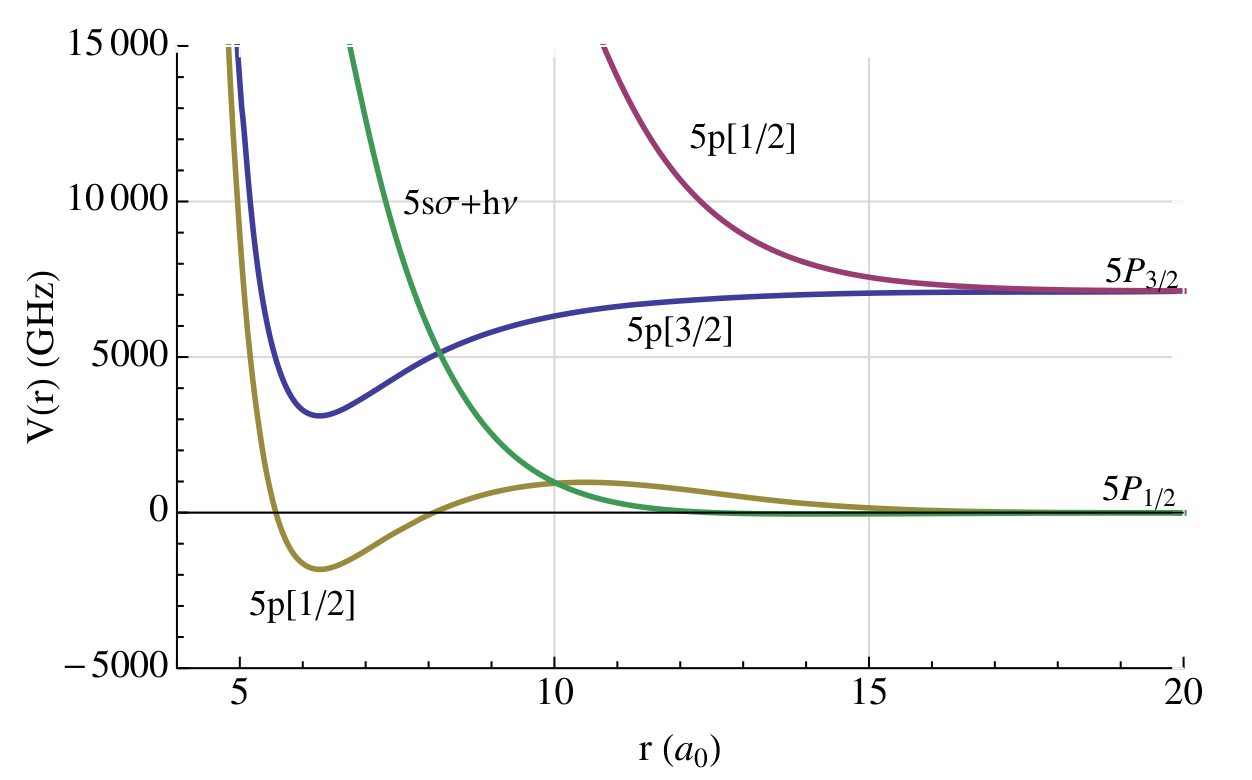
\includegraphics[width=\textwidth]{figures/chapter3-figs/OPalkalimixing.png}
    \caption[Atomic levels of Rb-$^3$He pair during optical pumping.]
    {Atomic levels of Rb-$^3$He pair during optical pumping. The figure shows the absorbtion of the D1 light crossing over with the mixed $5p[\frac{1}{2}]$ excited state. Figure is taken from \cite{Gentile2017} with the original calculations in \cite{Lancor2010}.}
    \label{fig:RbHepumping}
\end{figure}
\clearpage}

Since SEOP is intended for high density $^3$He cells, alkali-$^3$He collisions cause mixing of the alkali D1 atomic levels \cite{Lancor2010}. This is shown in \cref{fig:RbHepumping}. This allows for circularly polarized light to get absorbed in the mixed state, limiting the efficiency of optical pumping \cite{Lancor2010}. Thus, the alkali atoms can only achieve a maximum polarization, $P_{\infty}<1$, even under high optical pumping rates \cite{Lancor2010}.

\afterpage{
\begin{figure}
    \centering
    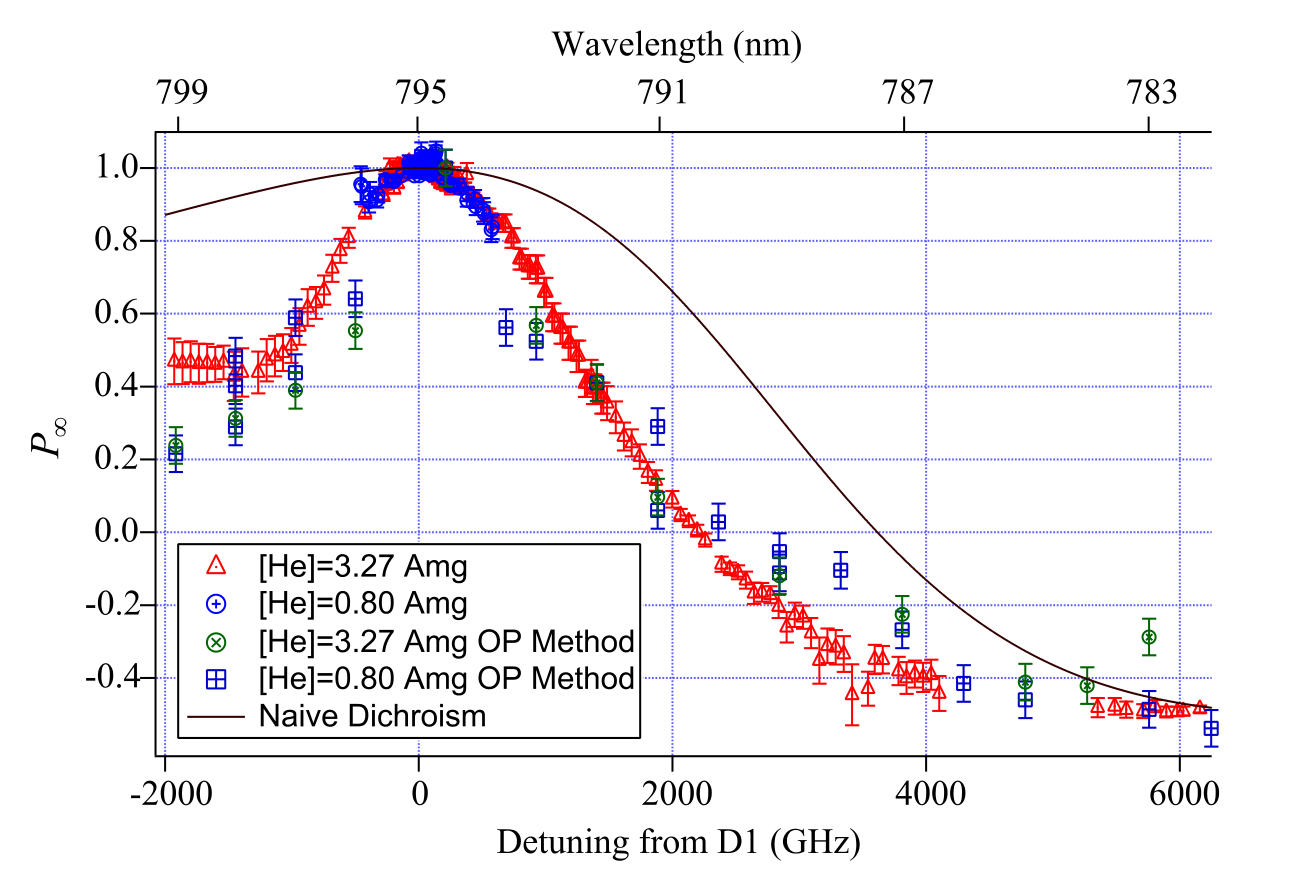
\includegraphics[width=\textwidth]{figures/chapter3-figs/dichroism.png}
    \caption[The maximum attainable alkali dichroism of Rb atoms in $^3$He.]{The maximum attainable alkali dichroism of Rb atoms in $^3$He. At the D1 resonance line of Rb, 795nm, the measured alkali polarization approaches 1. The solid line is the calculated dichroism without alkali-$^3$He collisions. Figure is taken from \cite{Gentile2017} with the original data in \cite{Lancor2010}.}
    \label{fig:dichroism}
\end{figure}
\clearpage}

\Cref{fig:dichroism} show measurement results of the dichroism\footnote{Dichroism means polarization dependent absorption.} of polarized Rb atoms in the presence of different densities of $^3$He \cite{Lancor2010}. The figure shows that while the alkali polarization peaks at the D1 resonance, a 1 nm detuning from the resonance drops the maximum alkali polarization to 0.9. This emphasizes the need for narrow-bandwidth lasers for yielding efficient optical pumping as well as higher maximum polarization.

The optical light scattering rate, $\mathcal{A}({\bf x})$, can be written as \cite{Gentile2017, Walker1997}:
\begin{equation}
\begin{split}
        \mathcal{A}({\bf x}) & = R({\bf x}) \left[ 1 - (P_{\infty}P_{A}) \right] \\
        & = \Gamma_A P_{\infty} P_{A}({\bf x}) - R({\bf x})(1-P_{\infty}^2)
\end{split}
\end{equation}
The first term compensates for collisions causing spin relaxation and the second term accounts for the light scattering from any off D1 line pumping \cite{Happer1987, Happer2010, Lancor2010}. In optical pumping, the light fluence rate or light flux density, $I({\bf x}) [cm^{-2}s^{-1}]$ at a location in the cell, {\bf x}, can be described as:
\label{eq:fluxdensity}
\begin{flalign}
    \frac{dI({\bf x})}{d{\bf x}} & = \mathcal{A}({\bf x})[A] \\ \nonumber
    & = [A]\Gamma_A P_{\infty} P_{A}({\bf x}) - [A]R({\bf x})(1-P_{\infty}^2) \\
    & = [A]\Gamma_A P_{\infty} P_{A}({\bf x}) - [A] \sigma_A I({\bf x})(1-P_{\infty}^2) \nonumber
    \label{eq:fluxdensity}
\end{flalign}
where [A] is the alkali concentration and the optical cross section, $\sigma_A$, for unpolarized alkali atoms is defined as the ratio of the optical pumping rate $R({\bf x})$ to the light flux density$I({\bf x})$ \cite{Appelt1998, Gentile2017}. If on D1 line pumping ($P_A \approx P_{\infty} = 1$), the first term in the equation leads to a linear attenuation in light flux density $I=I_0-[A]\Gamma_A P_{\infty}^2{\bf x}$ \cite{Bhaskar1979, Walker1997}. This means that the D1 light gets attenuated from the spin relaxation collisions despite the optical thickness of SEOP cells. If off D1 line pumping ($P_{\infty} < 1$), \cref{eq:fluxdensity} leads to an exponential attenuation of the light as $I=I_0 \exp \left ( - [A] \sigma (1-P_{\infty}^2){\bf x} \right )$ because the absorption length increases by a factor $\frac{1}{1-P_{\infty}^2}$ as compared to the absorption length under uniformly polarized alkali atoms \cite{Gentile2017}. 

Scattering of light also happens during off D1 line dichroism \cite{Babcock2003}. A light absorption efficiency defined as a the ratio of the production rate of polarized $^3$He to the light scattering \cite{Babcock2003}, can be used to characterize this:
\begin{equation}
    \eta_{\gamma} = \frac{[He]\frac{dP_{He}}{dt}}{[A]\mathcal{A}}
\end{equation}
where [He] is the concentration of He in the cell. Measured light absorption efficiency for optical pumping with a broad spectrum laser is shown in \cref{fig:lightefficiency}. This indicates that for optical pumping under off D1 line, the is light absorption becomes inefficient, due to light scattering \cite{Babcock2003}.

\afterpage{
\begin{figure}
    \centering
    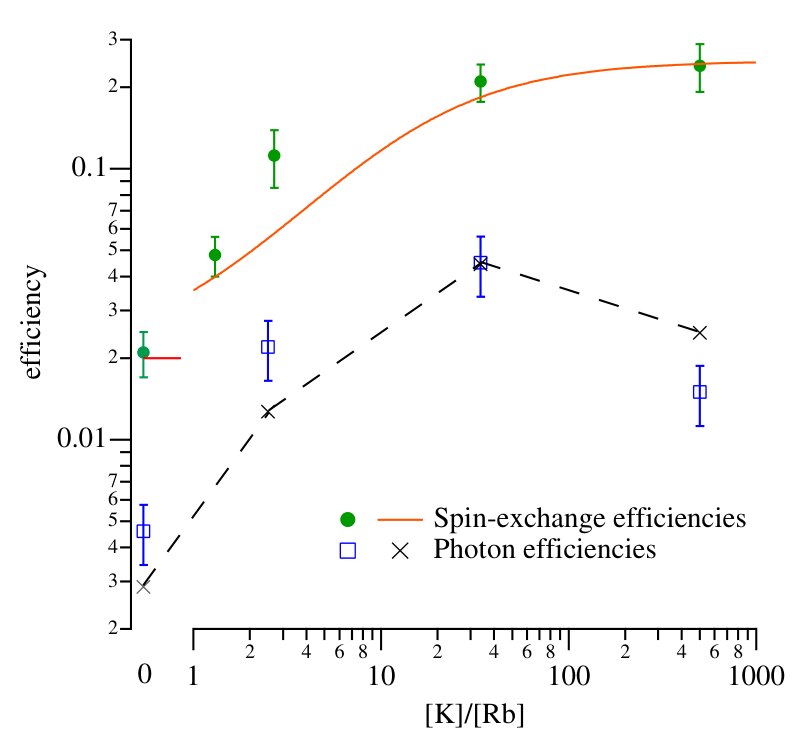
\includegraphics[width=\textwidth]{figures/chapter3-figs/SEeff_forD.png}
    \caption[Measured spin exchange and light absorption efficiencies as a function of alkali mixture concentration.]{Measured spin exchange and light absorption efficiencies as a function of alkali mixture concentration. The light absorption is  inefficient as compared to the maximum spin transfer efficiency due to the non-dichroism effects. Figure is taken from \cite{Gentile2017} with the original data and calculation from \cite{Babcock2003}.}
    \label{fig:lightefficiency}
\end{figure}
\clearpage}

In the early days, SEOP polarization of $^3$He used to struggle due to expensive, bulky, low power and broad spectral width laser technology \cite{Chupp1987, Wagshul1989, Coulter1990}. With the introduction of narrower laser diodes and compact Variable Bragg Gratings with integrated cooling systems in recent years, SEOP performance and attainable $^3$He polarization has increased \cite{Volodin2004, Chen2014}. These new lasers generally produce monochromatic light with a spectral width $<$ 0.2 nm (90 GHz), matching to the alkali D1 transition line, increasing the maximum attainable alkali polarization $P_{\infty}$. 

Other effects such as aberration of the incident laser light from uneven glass cells, changes in the laser beam divergence by glass and variation in the spatial modes of laser light can also prevent a uniform optical pumping rate along the volume of the cell \cite{Chann2003, Chen2014}. Although these factors can be somewhat mitigated by laser pumping the cell from both directions, a comprehensive study of the effect and mitigation of these factors on optical pumping has not been performed \cite{Chann2003, Chen2014}.


\subsection{Spin Exchange}

The exchange of spin angular momentum between the alkali and the $^3$He can be thought of as:
\begin{equation}
    A \uparrow + ^3He \downarrow \leftrightarrow A \downarrow + ^3He \uparrow
\end{equation}

The interaction potentials experienced during alkali-$^3$He collisions are
\begin{equation}
    V \propto V_0 + \Vec{S} \cdot \Vec{I}_{He} + \Vec{S} \cdot \Vec{N}
\label{eq:SEpot}
\end{equation}
where,
\begin{itemize}
    \item $V_0$ is the spin-independent interaction potential between the alkali-$^3$He \cite{Partridge2001, Tscherbul2011}.
    \item $\Vec{S} \cdot \Vec{I}_{He}$ is the hyperfine interaction between the alkali electron spin, $\Vec{S}$, and the $^3$He nuclear spin, $\Vec{I}_{He}$ \cite{Partridge2001, Tscherbul2011}.
    \item $\Vec{S} \cdot \Vec{N}$ is the alkali spin and alkali-$^3$He pair rotational angular momentum interaction \cite{Walker1997}. As discussed earlier, this is one of the known sources of spin relaxation in alkali and limits the spin exchange efficiency.
\end{itemize}

\afterpage{
\begin{figure}
    \centering
    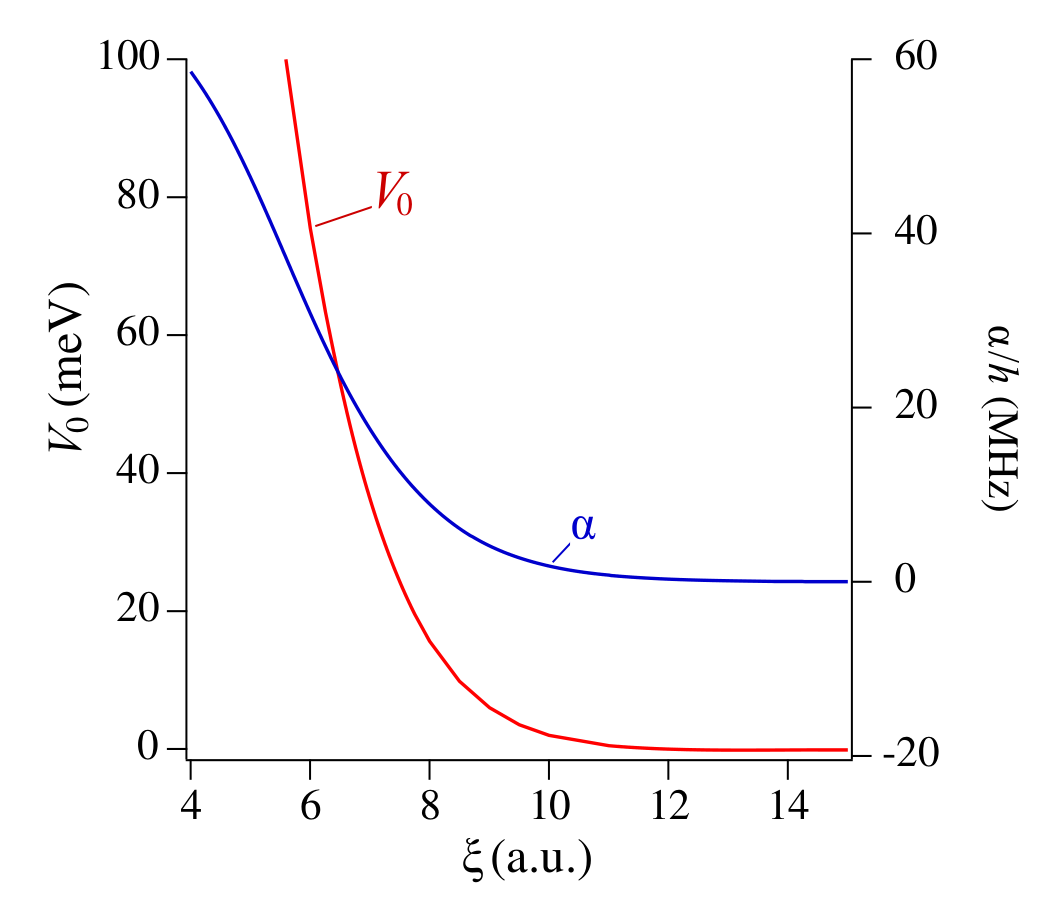
\includegraphics[width=\textwidth]{figures/chapter3-figs/SEpotentials.png}
    \caption[Calculated $V_0(x)$ and  $\Vec{S} \cdot \Vec{I_{He}}$ as a function of interatomic distance, $\xi$, for the K-$^3$He pair.]{Calculated $V_0(x)$ \cite{Partridge2001} and  $\Vec{S} \cdot \Vec{I_{He}}$ \cite{Tscherbul2011} for the K-$^3$He pair. Figure is taken from \cite{Gentile2017}.}
    \label{fig:spinexpot}
\end{figure}
\clearpage}

The interaction potentials, as shown in \cref{fig:spinexpot}, can be used to calculate the alkali-$^3$He spin-exchange rate, $k_{SE}$ \cite{Partridge2001, Tscherbul2011}. For K-$^3$He, the $k_{SE}$ comes out to be around $6 \times 10^{-20}$ cm$^3$s$^{-1}$ \cite{Gentile2017, Happer1972, Walker1997}. For typical alkali concentrations used in SEOP in the range of $10^{14}$ cm$^{-3}$ to $10^{15}$ cm$^{-3}$, the probability of spin exchange is very low and the spin-exchange time constant, $1/k_{SE}$, is around 10 to 50 hours \cite{Gentile2017}. This impresses the importance of building $^3$He cells with long lifetimes to achieve high $^3$He polarization.

The spin exchange and the relaxation/build up of polarized $^3$He, $P_{He}$, (mostly due to wall relaxation with rate, $\Gamma_{wall}$) can be modeled as \cite{Wu2021}:
\begin{equation}
    \frac{dP_{He}}{dt} = k_{SE} [A] (P_{A} -P_{He}) - \Gamma_{wall} P_{He}
\end{equation}
Since the $P_{He}$ varies on the scale of hours as compared to the alkali-metal electron polarization $P_{A}$, which varies with millisecond relaxation times, $P_{A}$ can be treated as constant. Thus, in a steady state solution, $P_{He}$ builds up as
\begin{equation}
    P_{He, \infty} = P_{A} \frac{k_{SE} [A]}{k_{SE} [A] + \Gamma_{wall}}
\end{equation}
at a time constant of
\begin{equation}
    \frac{1}{\tau} = k_{SE} [A] + \Gamma_{wall}
    \label{eq:SEtime}
\end{equation}
This linear relation implies that one can measure $k_{SE}$, and in effect the build up of $P_{He, \infty}$, by measuring the time constant as a function of the alkali concentration, [A] \cite{Gentile2017}. However, as will be described later, $\Gamma_{wall}$, has been found to vary non-linearly as a function of temperature of the $^3$He cell and only wall loss relaxation independent methods have to be used to measure $k_{SE}$ \cite{Gentile2017}. The no SEOP re-polarization method \cite{Ben-AmarBaranga1998, Chann2002a, Borel2003}, the rate balance method \cite{Chann2002a}, the $^4$He exchange rate method \cite{Walker2010}, and the absolute alkali polarimetry method \cite{Singh2015} have been used to measure the spin-exchange rate, $k_{SE}$ for the different alkali. The results from these measurements are shown in \cref{tab:spinexrate}

\afterpage{
\begin{table}
\centering
\caption[Measurements of spin-exchange rate coefficient using wall-independent methods all normalized to  the EPR frequency shift factors]{Measurements of spin-exchange rate coefficient $k_{SE}$, using wall-independent methods, all normalized to the EPR frequency shift factors $\kappa_0$ and $\frac{d\kappa_0}{dT}$. Data taken from \cite{Ben-AmarBaranga1998, Chann2002a, Borel2003, Walker2010, Singh2015}.}
\label{tab:spinexrate}
\begin{tabular}{@{}lccc@{}}
\toprule
 & Na & K & Rb \\ \midrule
$k_{SE} $ [$10^{-20}$ cm$^{3}$s$^{-1}$] & 6.1 & 6.1-7.5 & 6.7-6.8 \\
$\kappa_0$ & 4.7 & 6.0 & 6.1 \\
$\frac{d\kappa_0}{dT}$ [K$^{-1}]$ & 0.009 & 0.008 & 0.009 \\ \bottomrule
\end{tabular}
\end{table}
\clearpage}

Even though the spin exchange from alkali to $^3$He is limited with a slow time constant, the efficiency of the optically pumping to polarize the alkali is high. If no light scattering from polarized alkali atoms is assumed, the loss of angular momentum by polarized alkali-metal atoms happens at a rate [A] V $\Gamma_A P_A$. At the same time, the addition of angular momentum to $^3$He happens as,  V[He]$\frac{dP_{He}}{dt}$, the spin exchange collision efficiency can be written as \cite{Gentile2017, Ben-AmarBaranga1998}:
\begin{equation}
    \eta = \frac{V [He] \frac{dP_{He}}{dt}}{[A] V \Gamma_A P_A} = \frac{k_{SE} [He]}{\Gamma_A} \left (  1- \frac{P_{He}}{P_{He, \infty}}             \right )
\end{equation}

This spin exchange collision efficiency is maximum during the early stages of SEOP at low $^3$He polarization, but then decreases as higher $^3$He polarization and alkali polarization approach equilibrium. This efficiency varies from alkali to alkali \cite{Ben-AmarBaranga1998}.

Although $\Gamma_A$ contributes to the alkali spin-relaxation rate, the minimum possible alkali spin-relaxation rate is $\Gamma_A = (k_{SE} + k_{SR}) $[He] , where $k_{SR}$ is the relaxation due to the the alkali spin and alkali-$^3$He pair rotational angular momentum interaction as discussed previously \cite{Ben-AmarBaranga1998, Borel2003, Singh2010}. This relaxation limits the spin exchange to:
\begin{equation}
    \eta = \frac{k_{SE}}{k_{SE} + k_{SR}}
\end{equation}
Measurements and expected values of the spin-exchange efficiency for the alkali elements, Na, K, Rb and Cs are shown in \cref{fig:SEeff}.

\afterpage{
\begin{figure}
    \centering
    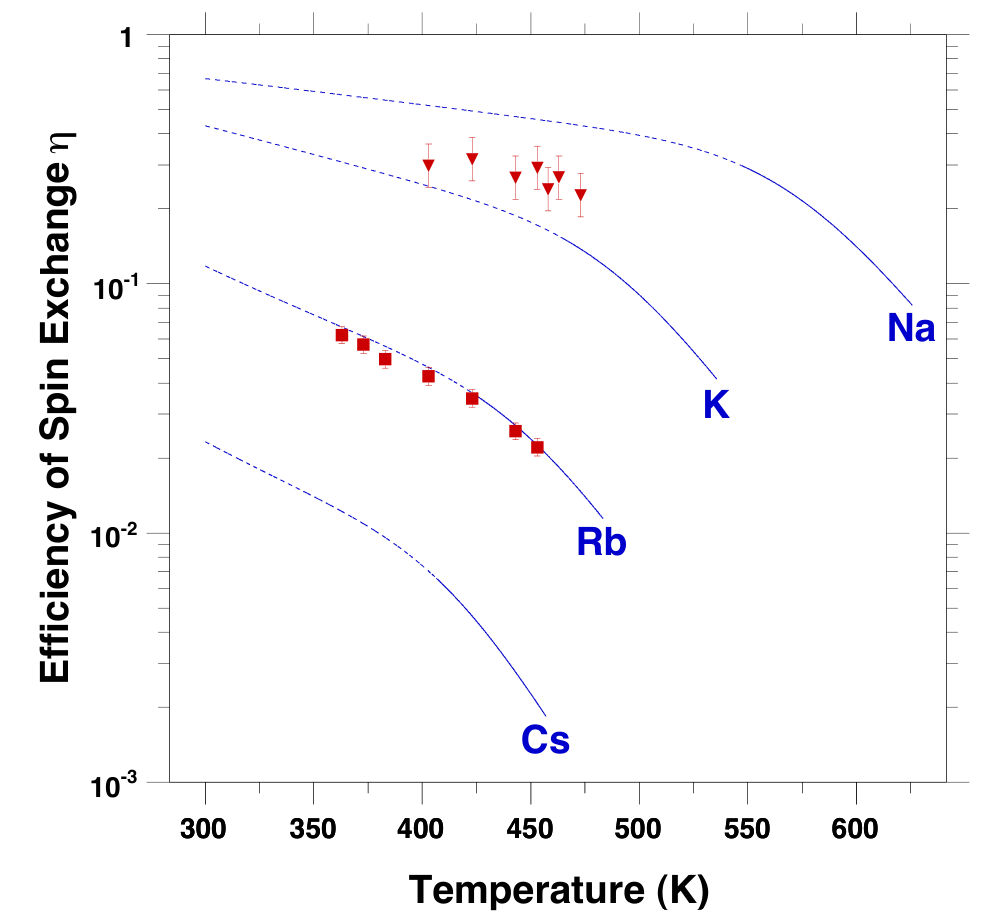
\includegraphics[width=\textwidth]{figures/chapter3-figs/SEeff.png}
    \caption[Spin Exchange Efficiencies for Na, K, Rb, \& Cs]{Spin Exchange Efficiencies for Na, K, Rb, \& Cs taken from \cite{Singh2010}. The blue lines are calculated from \cite{Singh2010} and the red data points are from \cite{Ben-AmarBaranga1998}. The SEOP described in the thesis performed at $^3$He cell temperature of 200 \degree C so the efficiency curves shown in this plot have to be extrapolated at those temperatures. Nonetheless, the efficiency trends shown in this figure looks to match the efficiency at 200 \degree C.}
    \label{fig:SEeff}
\end{figure}
\clearpage}

\subsection{SEOP with Hybrid Alkali}

\Cref{fig:SEeff} shows that of all the alkali elements, Na and K have the largest spin exchange efficiency as compared to Rb and Cs. Therefore, it is sensible to pursue SEOP using Na or K alkali atoms.\footnote{In terms of neutron scattering and absorption, Na, K, Rb can be used due to small neutron scattering and absorption cross sections. For Cs, the scattering cross section is a little large.} However, It is not yet possible to perform SEOP using Na because of the technological unavailability of 590 nm lasers at the D1 transitions of Na \cite{Borel2003}. This leaves us with K and Rb. Direct pumping of pure K based cells is also difficult due to potential unwanted optical pumping of the K D2 line in the fine-structure \cite{Chen2007}. Although at the level of 0.2 nm spectral width, 770 nm K D1 transition lasers have not yet reached $>$ 100 W power levels, \cite{Chen2007} found increased spin exchange efficiency using hybrid (K and Rb) alkali cells and this has become the standard approach for polarizing $^3$He using SEOP for neutron spin filters \cite{Chen2007, Chen2011}.  
In hybrid SEOP, a Rb/K mixture cells are used with higher concentration of K as compared to Rb \cite{Lancor2010, Lancor2011}. The Rb is optically pumped based on the Rb D1 line. Alkali-alkali spin-exchange leads the K atoms to become polarized as well. Since K has a smaller spin relaxation rate than Rb, the K-$^3$He spin exchange of angular momentum is more efficient as compared to Rb \cite{Lancor2010, Lancor2011}. Taking into account the total hybrid alkali spin-relaxation rate $\Gamma_{Rb}$ + $ \mathcal{D}$  $ \Gamma_K$, where $ \mathcal{D} $ = [K]/[Rb], the hybrid alkali spin-exchange efficiency becomes:
\begin{equation}
    \eta^{hybrid} = \frac{ (k_{SE}^{Rb} + \mathcal{D} k_{SE}^{K} ) [He]}{\Gamma_{Rb} + \mathcal{D}\Gamma_K}
\end{equation}
which for large $\mathcal{D}$, approaches $\eta_{SE}^{K}$ \cite{Lancor2010, Lancor2011}. This can be seen in the measurements of the spin-exchange efficiency for different concentrations of alkali mixture shown in \cref{fig:hybrideff}.

\afterpage{
\begin{figure}
    \centering
    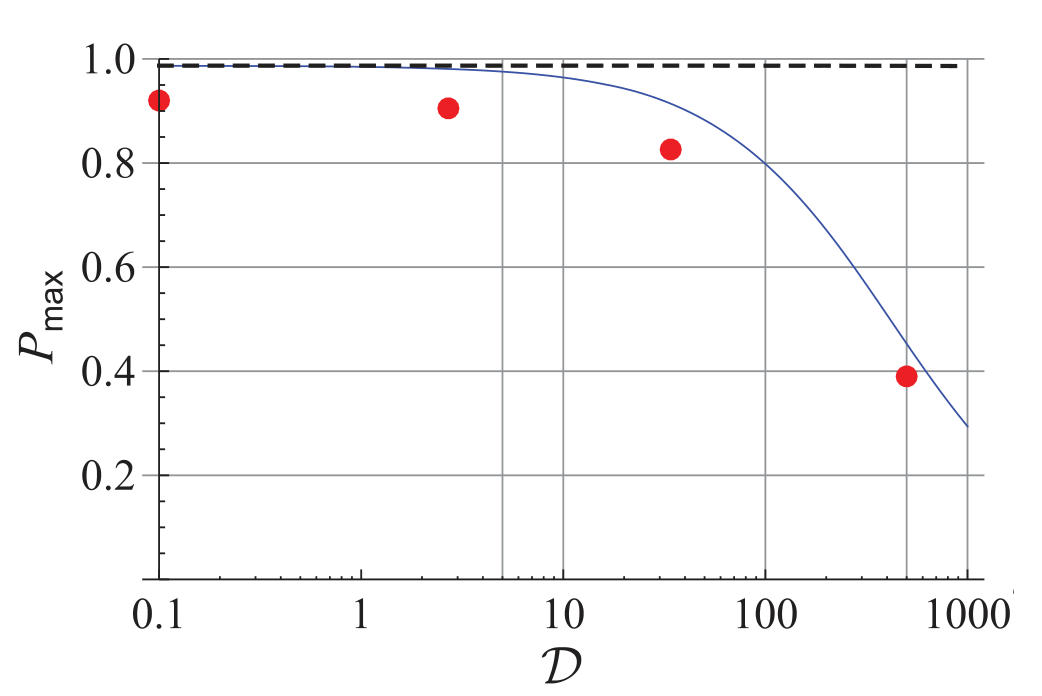
\includegraphics[width=\textwidth]{figures/chapter3-figs/Pmax_vs_D.png}
    \caption[Alkali polarization as a function of alkali ratio.]{Alkali polarization as a function of alkali mixture. Figure is taken from \cite{Gentile2017} with the original data in \cite{Lancor2010, Lancor2011}.}
    \label{fig:hybrideff}
\end{figure}
\clearpage}

The reduction in loss from collisions in hybrid SEOP allows for an increased alkali density and thus, an increased polarization rate and furthermore, a large volume of $^3$He to be polarized. $\mathcal{D}$ ratio between 2 and 7 is found to yield the best spin exchange efficiency \cite{Chen2007, Chen2011, Chen2014}. For neutron based $^3$He cells, $\mathcal{D}$ usually determined with relative peak intensities in white light absorption spectroscopy as well as monitoring optical pumping rate as a function of temperature \cite{Chen2007, Chen2011, Chen2014}.

\subsection{$^{3}$He Relaxation Mechanisms}

This section describes the mechanisms responsible for `relaxing', i.e. depolarizing the polarized $^3$He. The primary mechanisms are the dipole-dipole relaxation, wall effects and field gradients.

\cite{Newbury1993} found that $T_1$ longitudinal polarization relaxation time, characterizes relaxation of $^3$He polarized along the direction of holding magnetic field is limited by the dipole-dipole interactions within $^3$He to $\frac{1}{T_1} = \frac{P}{807} $ hours$^{-1}$, where P is pressure of the cell in bars. This relaxation, which occurs as $\exp(-t/T_1)$, has been verified for $^3$He cells with pressures of 2 to 12 bars \cite{Smith1998}. For neutron spin filters made of GE180 glass, with pressures of $\sim$1bar and polarized via Rb or K-Rb SEOP, $T_1$ of several hundred hours has been observed \cite{Rich2002, Parnell2009, Chen2011}, and most likely attributed to formation of thin films of alkali coating the inner walls of the glass; suppressing wall relaxation \cite{Wu2021}.

A major limiting factor for a high achievable $T_1$ in a SEOP cell is the relaxation of polarized $^3$He with the glass cell walls. Yet, this effect is not fully understood despite being recognized since the very first SEOP $^3$He polarization experiment, where aluminosilicate glass yielded long relaxation times as compared to borosilicate glass \cite{Fitzsimmons1969}. Further studies have shown that $^3$He permeates the borosilicate glass whereas it adsorbs on the aluminosilicate glass \cite{Jacob2003, Gentile2017}. For aluminosilicate glass cells, longer $T_1$ time has been observed for cells kept at higher temperatures due to reduced adsorption on top of already negligible permeation \cite{Jacob2003}. This fact has led aluminosilicate glass based cells to become the standard for SEOP \footnote{Aluminosilicate glass is also resistant to alkali corrosion.}. For neutron beam based applications of $^3$He glass cells, this is incredibly useful because this avoids any attenuation of the neutron beam from possible boron content in the glass. It has also been found that tempered cells made from glass blowing, have been found to decrease $^3$He relaxation \cite{Rich2002, Parnell2009, Chen2011}.

Strong holding magnetic fields and physical orientation of the cell relative to the holding magnetic fields have also been found to have an effect on $^3$He relaxation. \cite{Chen2011} observed an order of magnitude decrease in $T_1$ with a holding field of 400 G. Interestingly, a ``hysteresis" was observed, where once 10 G to 30 G holding fields were applied, the high $T_1$ time was recovered. They also observed that $T_1$ can change, preferring to increase for a certain cell orientation i.e. $^3$He cells prefers to polarize only in certain physical orientations. 

The main culprit responsible for relaxation of polarized $^3$He in SEOP cells is presence of magnetic field gradients transverse to the holding field $B_0$, which causes the $^3$He polarization spins to precess non-adiabatically away from $B_0$ \cite{Gamblin1965, Schearer1965, Cates1988a, Cates1988b, McGregor1990, Bohler1994}. At room temperature and pressure, P in bars, a useful relation for the relaxation rate caused by a field gradient, in units of hours$^{-1}$, is given by \cite{McIver2009}:
\begin{equation}
    \frac{1}{T_1} = \frac{6700}{P} \left ( \frac{\left \lvert \Vec{\nabla} B_{\perp} \right \rvert ^2}{B_0^2} \right )
\label{eq:gradT1}
\end{equation}
where $ \frac{ \left \lvert \Vec{\nabla} B_{\perp} \right \rvert}{B_0}$ is the transverse gradient in the longitudinal magnetic field, in units of cm$^{-1}$, assuming longitudinal polarization is along the z-axis \cite{Cates1988b}. For a 1 bar cell in a uniform gradient of
\begin{equation}
     \frac{ \left \lvert \Vec{\nabla} B_{\perp} \right \rvert}{B_0} \approx 3 \times 10^{-4}  ~\text{cm$^{-1}$}
\label{eq:gradstandard}
\end{equation}
the $^3$He polarization relaxation time, from the \cref{eq:gradT1}, comes out to be about 800 hours \footnote{This relation is only valid for when the $ \omega_{Larmor}^{He} \ll \frac{1}{\tau_{collisions}}$.} \cite{Chen2020}. This relaxation time is usually adequate for SEOP cells used in neutron based experiments and so the gradients listed in \cref{eq:gradstandard} are usually the standards for developing magnetostatic cavities for providing the uniform holding magnetic fields for the polarized $^3$He cell. In conjunction with the need for low field gradients, space constraints, stray fields, and neutron spin transport magnetic field matching have also motivated the development of novel magnetostatic cavities for polarized $^3$He gas. Magnetically shielded solenoids and coils are typically employed to achieve this. Magnetic shielding and uniformity is provided via high magnetic permeability materials like mu-metal. $\cos \theta$ coils, double $\cos \theta$ coils and Merrit coils \cite{Merritt1983, Babcock2019, Chen2020}, enveloped by mu-metal shielding, have been used recently to achieve gradients between $6 \times 10^{-4} $ cm$^{-1}$ and $2 \times 10^{-4} $ cm$^{-1}$, corresponding to $^3$He polarization relaxation times between nearly 600 hours and 4000 hours, respectively \cite{Chen2014}.

\subsection{Limitations to $^{3}$He Polarization}

The previous sections describe how polarizing alkali via optical pumping, making glass cells with long wall-relaxation times, making making holding magnetic fields with low gradients, and utilizing hybrid alkali optical pumping for efficient spin exchange, should lead to very high $^3$He polarizations. In this section, the known systematic effects, which limit the maximum attainable $^3$He polarization are described.  

There is an anisotropic spin exchange alkali-$^3$He interaction, caused by the long-range $^3$He nuclear magnetization,
\begin{equation}
    V \propto  \Vec{S} \cdot \Vec{I_{He}}
\end{equation}
which polarizes the $^3$He nuclei as $ P_{He} \propto - P_A $, and therefore, limits the maximum attainable $^3$He polarization as
\begin{equation}
    P_{He, \infty} \le 1 - \frac{3 k_{S\cdot I}}{ 2 k_{hf}}
\end{equation}
Here $k_{hf}$ is the rate coefficient due to the hyperfine interaction from \cref{eq:SEpot} and $k_{S\cdot I}$ is the rate coefficient due to the anisotropic interaction \cite{Walter1998}. A calculation of this interaction limits the maximum attainable $^3$He polarization to $P_{He, \infty} \approx 0.95$ for SEOP \cite{Walter1998, Tscherbul2011}. So far, there have been no definitive measurements of anisotropic spin exchange contribution towards $^3$He polarization.

\afterpage{
\begin{figure}
    \centering
    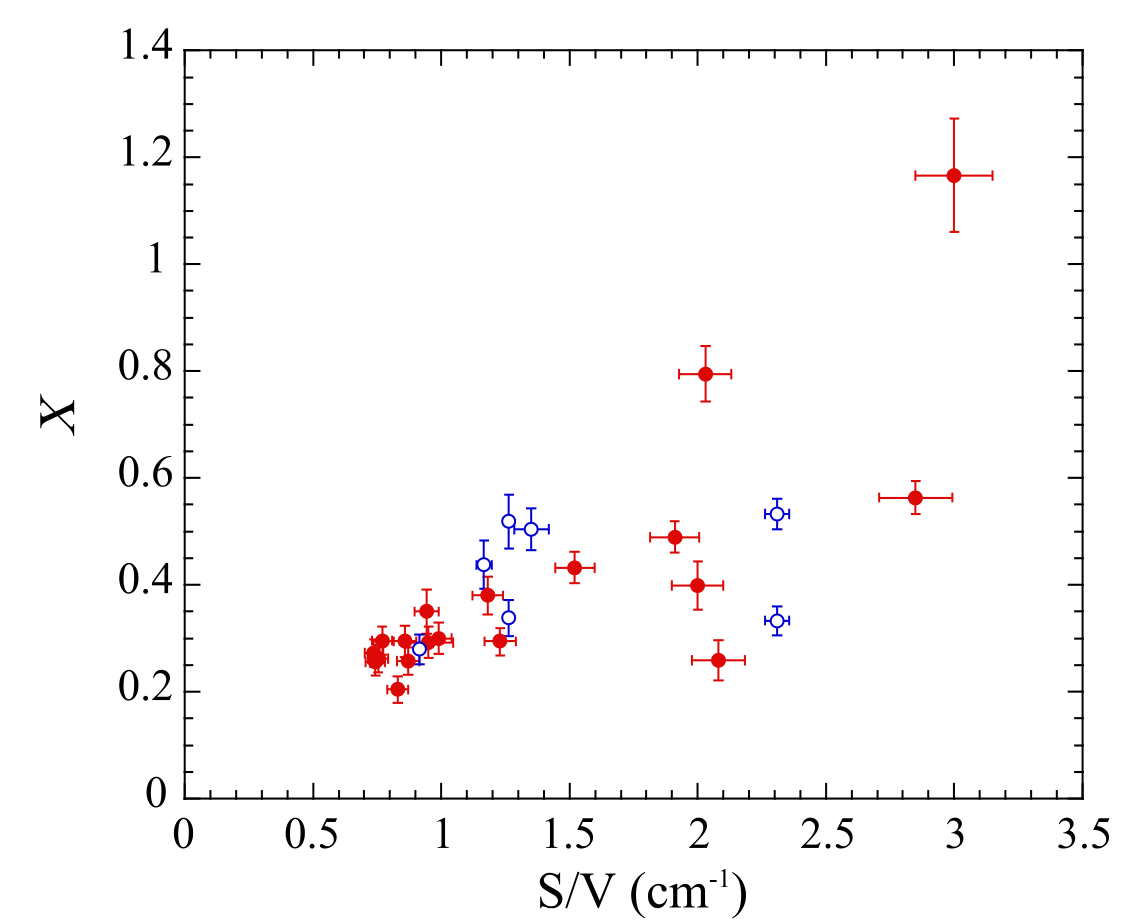
\includegraphics[width=\textwidth]{figures/chapter3-figs/Xfactor.png}
    \caption[Characterization of the X factor for spherical glass cells (red) and cylindrical glass cells (blue) as a function of the cell surface area to volume ratio.]{Characterization of the X factor for spherical glass cells (solid, red) and cylindrical glass cells (open, blue) as a function of the cell surface area to volume ratio. Figure is taken from \cite{Gentile2017} and the measurements were performed at NIST \cite{Babcock2006}.}
    \label{fig:Xfactor}
\end{figure}
\clearpage}

The second systematic effect, which limits the $^3$He polarization, is called the ``X-factor". Phenomenological studies of the spin exchange characteristic time, \cref{eq:SEtime}, use the relation:
\begin{equation}
    \frac{1}{\tau} = k_{SE} (1 + X) [A] + \Gamma_{wall}
\end{equation}
where $\Gamma_{wall}$ is the room temperature relaxation rate \cite{Chann2002a, Chann2003, Babcock2006, Chen2007, Walker2011, Chen2014, Singh2015}. This relation arises from the fact that the polarized $^3$He wall-relaxation rate has an excess term which increases exponentially as a function of temperature \cite{ Chann2003, Babcock2006, Walker2011, Chen2014, Singh2015}. This term limits the $^3$He polarization to
\begin{equation}
    P_{He, \infty} \le \frac{1}{1+X}
\end{equation}
assuming full alkali polarization and neglecting $\Gamma_{wall}$. This ``X factor", has been verified experimentally for both pure and hybrid cells with large variations across many different cells \cite{Chann2002a, Chann2003, Babcock2006, Chen2007, Walker2011, Chen2014, Singh2015}. This variation is what hints towards a possible temperature dependence, however the true cause of this effect is still unknown \cite{Chann2002a, Chann2003, Babcock2006, Chen2007, Walker2011, Chen2014, Singh2015}. Direct measurements of the ``X factor" have been performed by measuring the $^3$He relaxation in heated cells by parameterizing the ``X factor" as a function of the ratio of the surface area of cell to cell volume \cite{Babcock2006}. They are shown in \cref{fig:Xfactor}. These measurements were consistent with the highest possible $^3$He polarization observed so far of 75\% to 80\% \cite{Parnell2009, Ye2010, Singh2015}.

The third effect which can limit the $^3$He polarization is the fact that the $^3$He polarization is restricted by the spatial distribution of polarized alkali, especially when spin relaxation rates are negligibly small compared to spin exchange rates \cite{Gentile2017, Anderson2020}. Due to the high pressures used in SEOP, the diffusion of polarized alkali in the cell volume can be small, which means all regions of the cell must be illuminated by the laser for a useful SEOP. It is also important to characterize the spectrum of the residual transmitted light from the cell, verifying the depletion of D1 line laser light \cite{Lancor2011}.

\section{In situ Polarized $^{3}$He Cell}

As mentioned earlier in this chapter, polarized $^3$He cells can be thought of as a neutron spin filter (NSF) with the purpose of either producing beams of spin-polarized low-energy neutrons, or analyzing the spin-polarized state of a neutron beam. \cite{Ioffe2011}. The NSF’s ability to do this with near very good spin contrast comes from the spin dependence of the $^3$He neutron absorption cross section \cite{Coulter1990, Passell1966}. Other devices such as supermirrors \cite{Mezei1976} and Heusler crystals can also be used to provide near perfect neutron polarization and spin analysis \cite{Williams1988}. However, the operation of these devices is highly dependent upon the angular divergence and wavelength of the neutron beam. In contrast, NSFs are advantageous because they allow for the spin polarization to be decoupled from these beam effects. 

%Recently, there has been an increase in deploying in situ SEOP based NSF systems at the neutron beamline. These systems have a built-in oven for heating, an embedded laser system along with the optics, internal NMR system for polarized $^3$He control, and a magnetostatic cavity to provide the holding magnetic field.

$^3$He cells or NSFs are usually polarized by SEOP or MEOP in dedicated optical pumping stations in external laboratories \cite{Jiang2023}. After the $^3$He cell is polarization, the cell is relocated to the neutron experiment in a portable magnetostatic cavity \footnote{Neutron beam polarimetry for former experiments at the SNS beamline 13 was performed using $^3$He cells polarized off site.}. This ex situ deployment of polarized $^3$He has a problem: The $^3$He polarization undergoes exponential decay as soon as SEOP is turned off \cite{Jiang2023}. This decaying $^3$He polarization will inhibit the $^3$He cell's efficacy as a NSF, making it useful only for a limited time \cite{Jiang2017, Jiang2023}. Afterwards, the cell must return to the external optical pumping station for repolarization \cite{Jiang2017, Jiang2023}. Since the neutron polarization and transmission are changing with the decaying $^3$He polarization, the data analysis also becomes complicated. An in situ SEOP $^3$He polarization system would keep the saturated $^3$He cell polarization stable since the polarized $^3$He would undergo SEOP continuously, and not decay. Recently, SEOP-based compact in situ polarized $^3$He neutron spin filters have been developed to be utilized for neutron beam experiments at the Oak Ridge National Laboratory (ORNL) \cite{Tong2012, Jiang2014, Jiang2017, Jiang2023}. These systems can be deployed directly at the neutron beamline. In this section, the setup, assembly and performance testing of an in situ $^3$He polarizer for the beamline 13A is described.

The design model for the in situ $^3$He SEOP polarizer is shown in \cref{fig:insitu_side}. It is designed so that the neutron beam will traverse through the sapphire beam portals without any interference with the SEOP components as indicated in the \cref{fig:insitu_topdown}. \Cref{fig:insitupic} shows the in situ system undergoing assembly and performance at the SNS laser laboratory. The main components of the in situ system are (i) the laser head and interlocked laser enclosure, (ii) the cell heating system (iii) the light optics and (iv) the magnetic field coil and shielding.

\afterpage{
\begin{figure}
    \centering
    \begin{subfigure}[b]{0.8\textwidth}
        \centering
         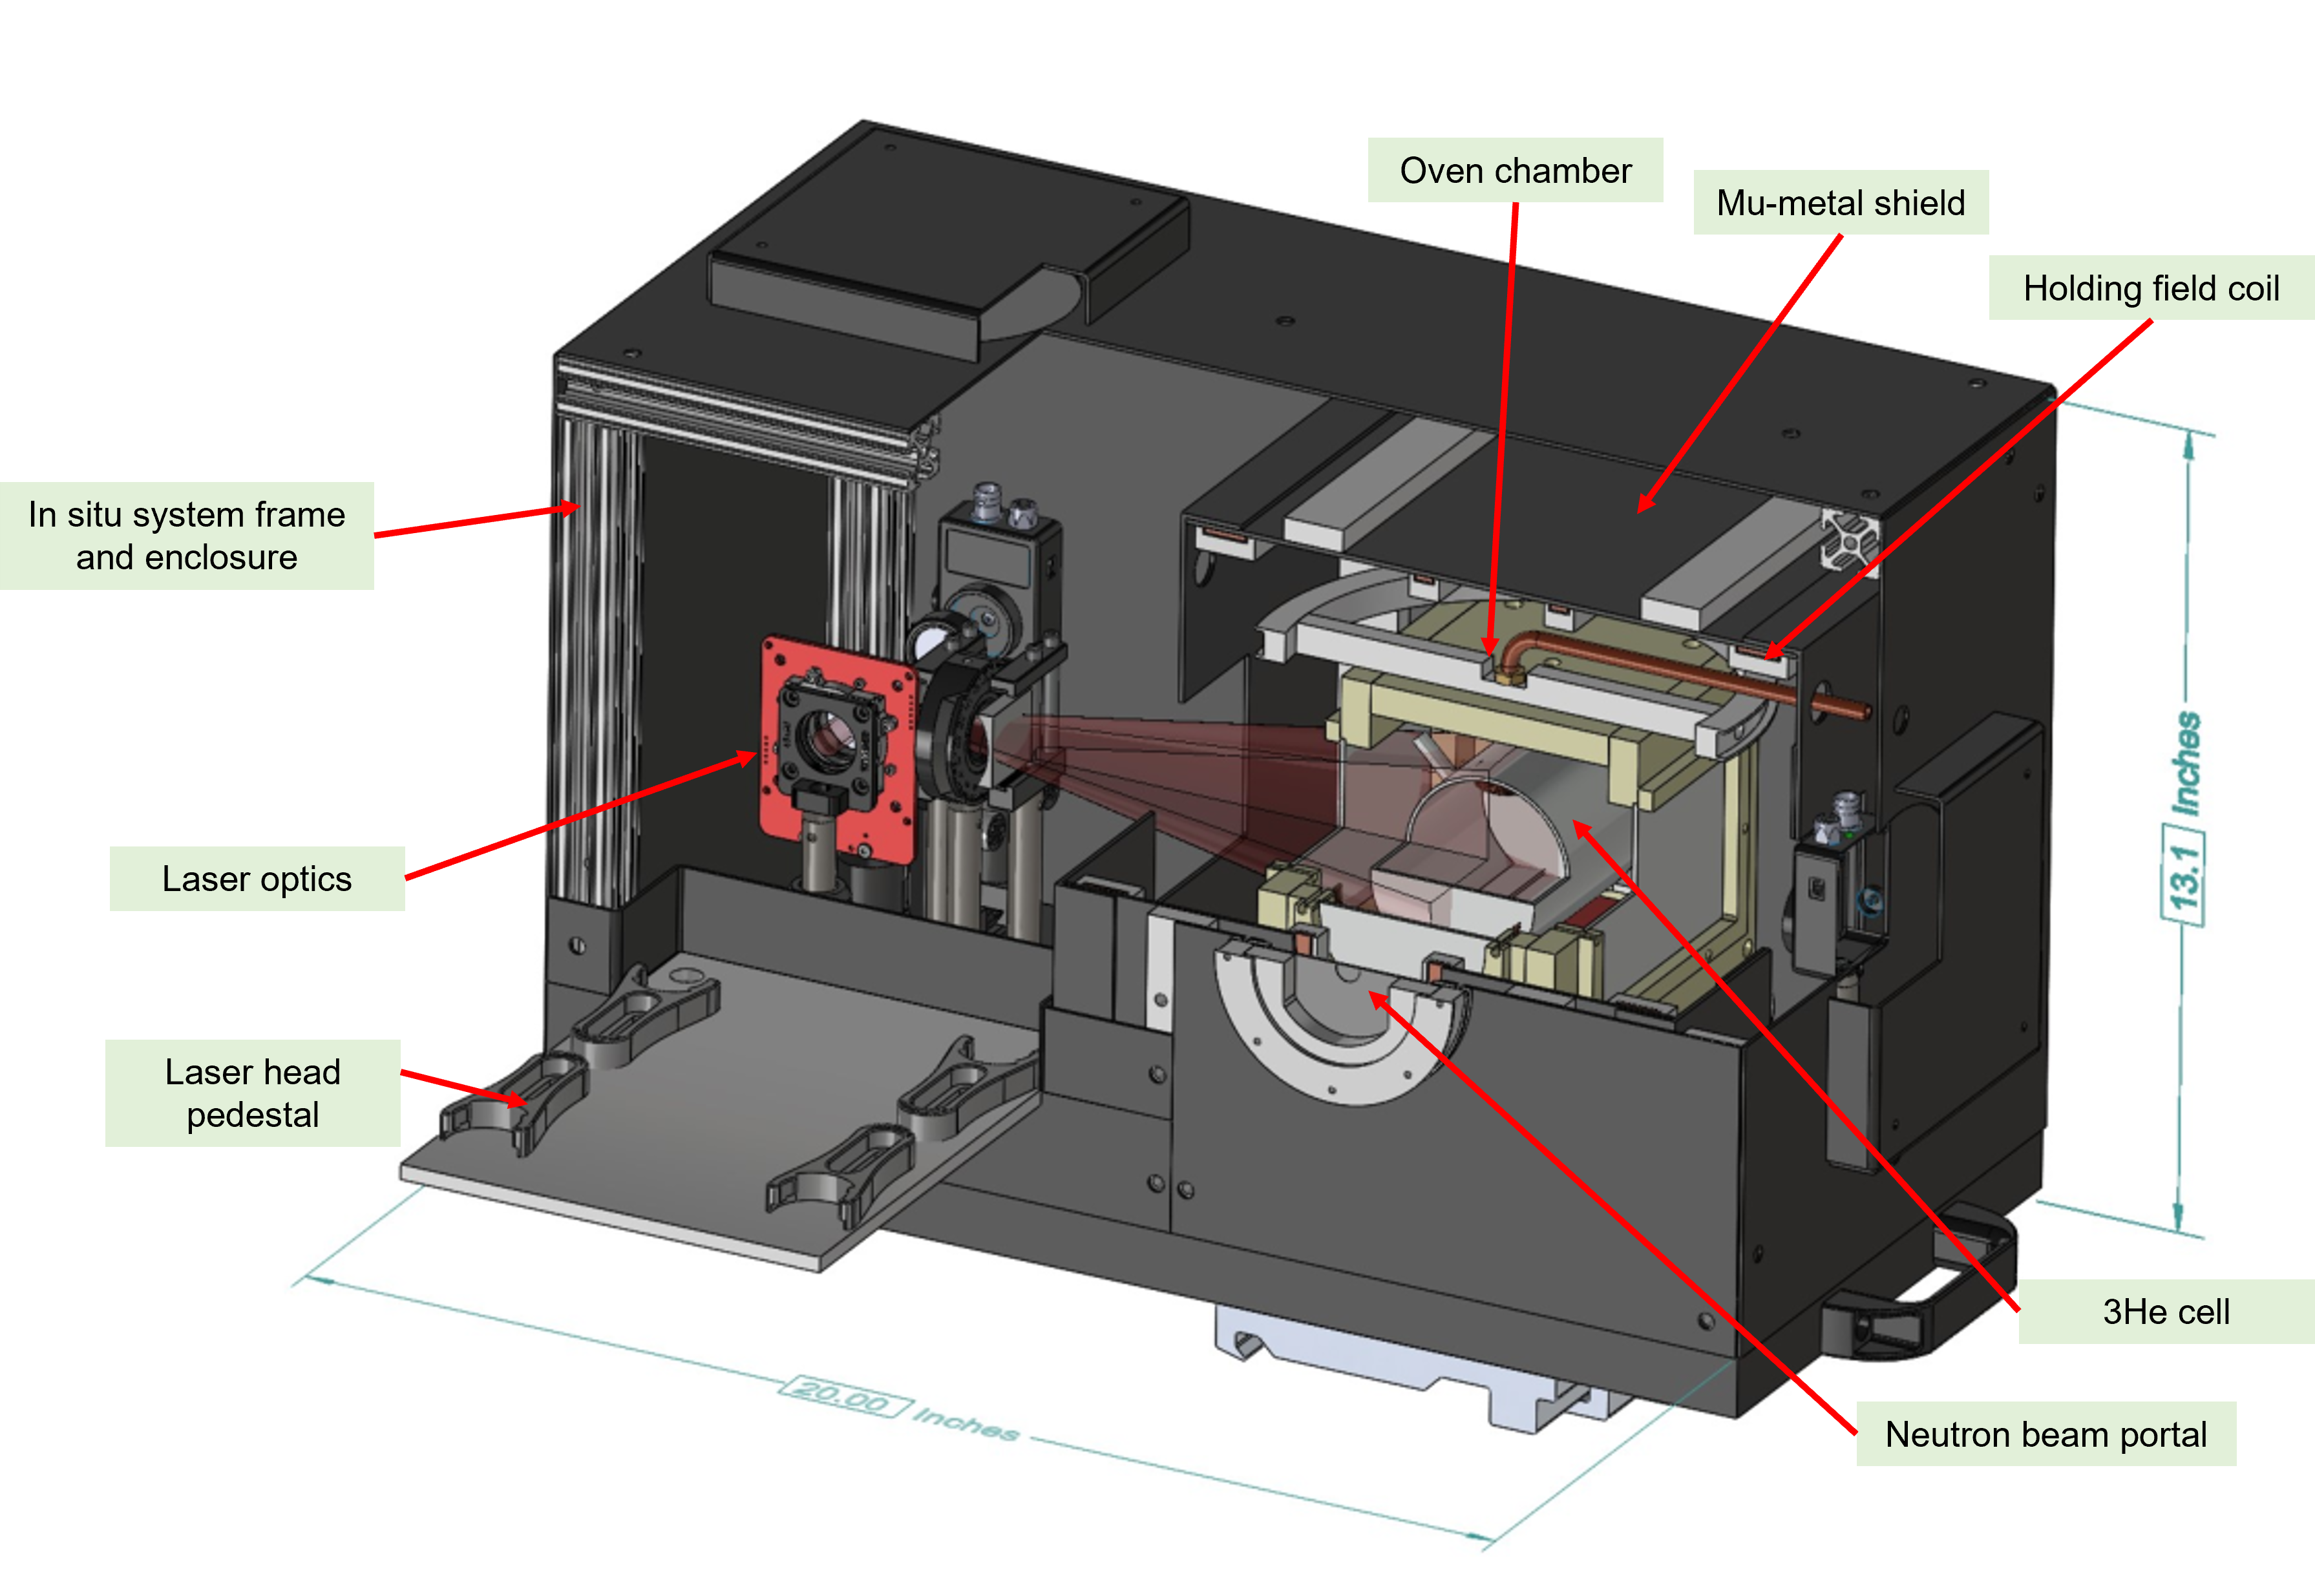
\includegraphics[width=\textwidth]{figures/chapter3-figs/insitumodel.png}
         \caption{Side view.}
         \label{fig:insitu_side}
     \end{subfigure}
     \hfill
     \begin{subfigure}[b]{0.8\textwidth}
        \centering
         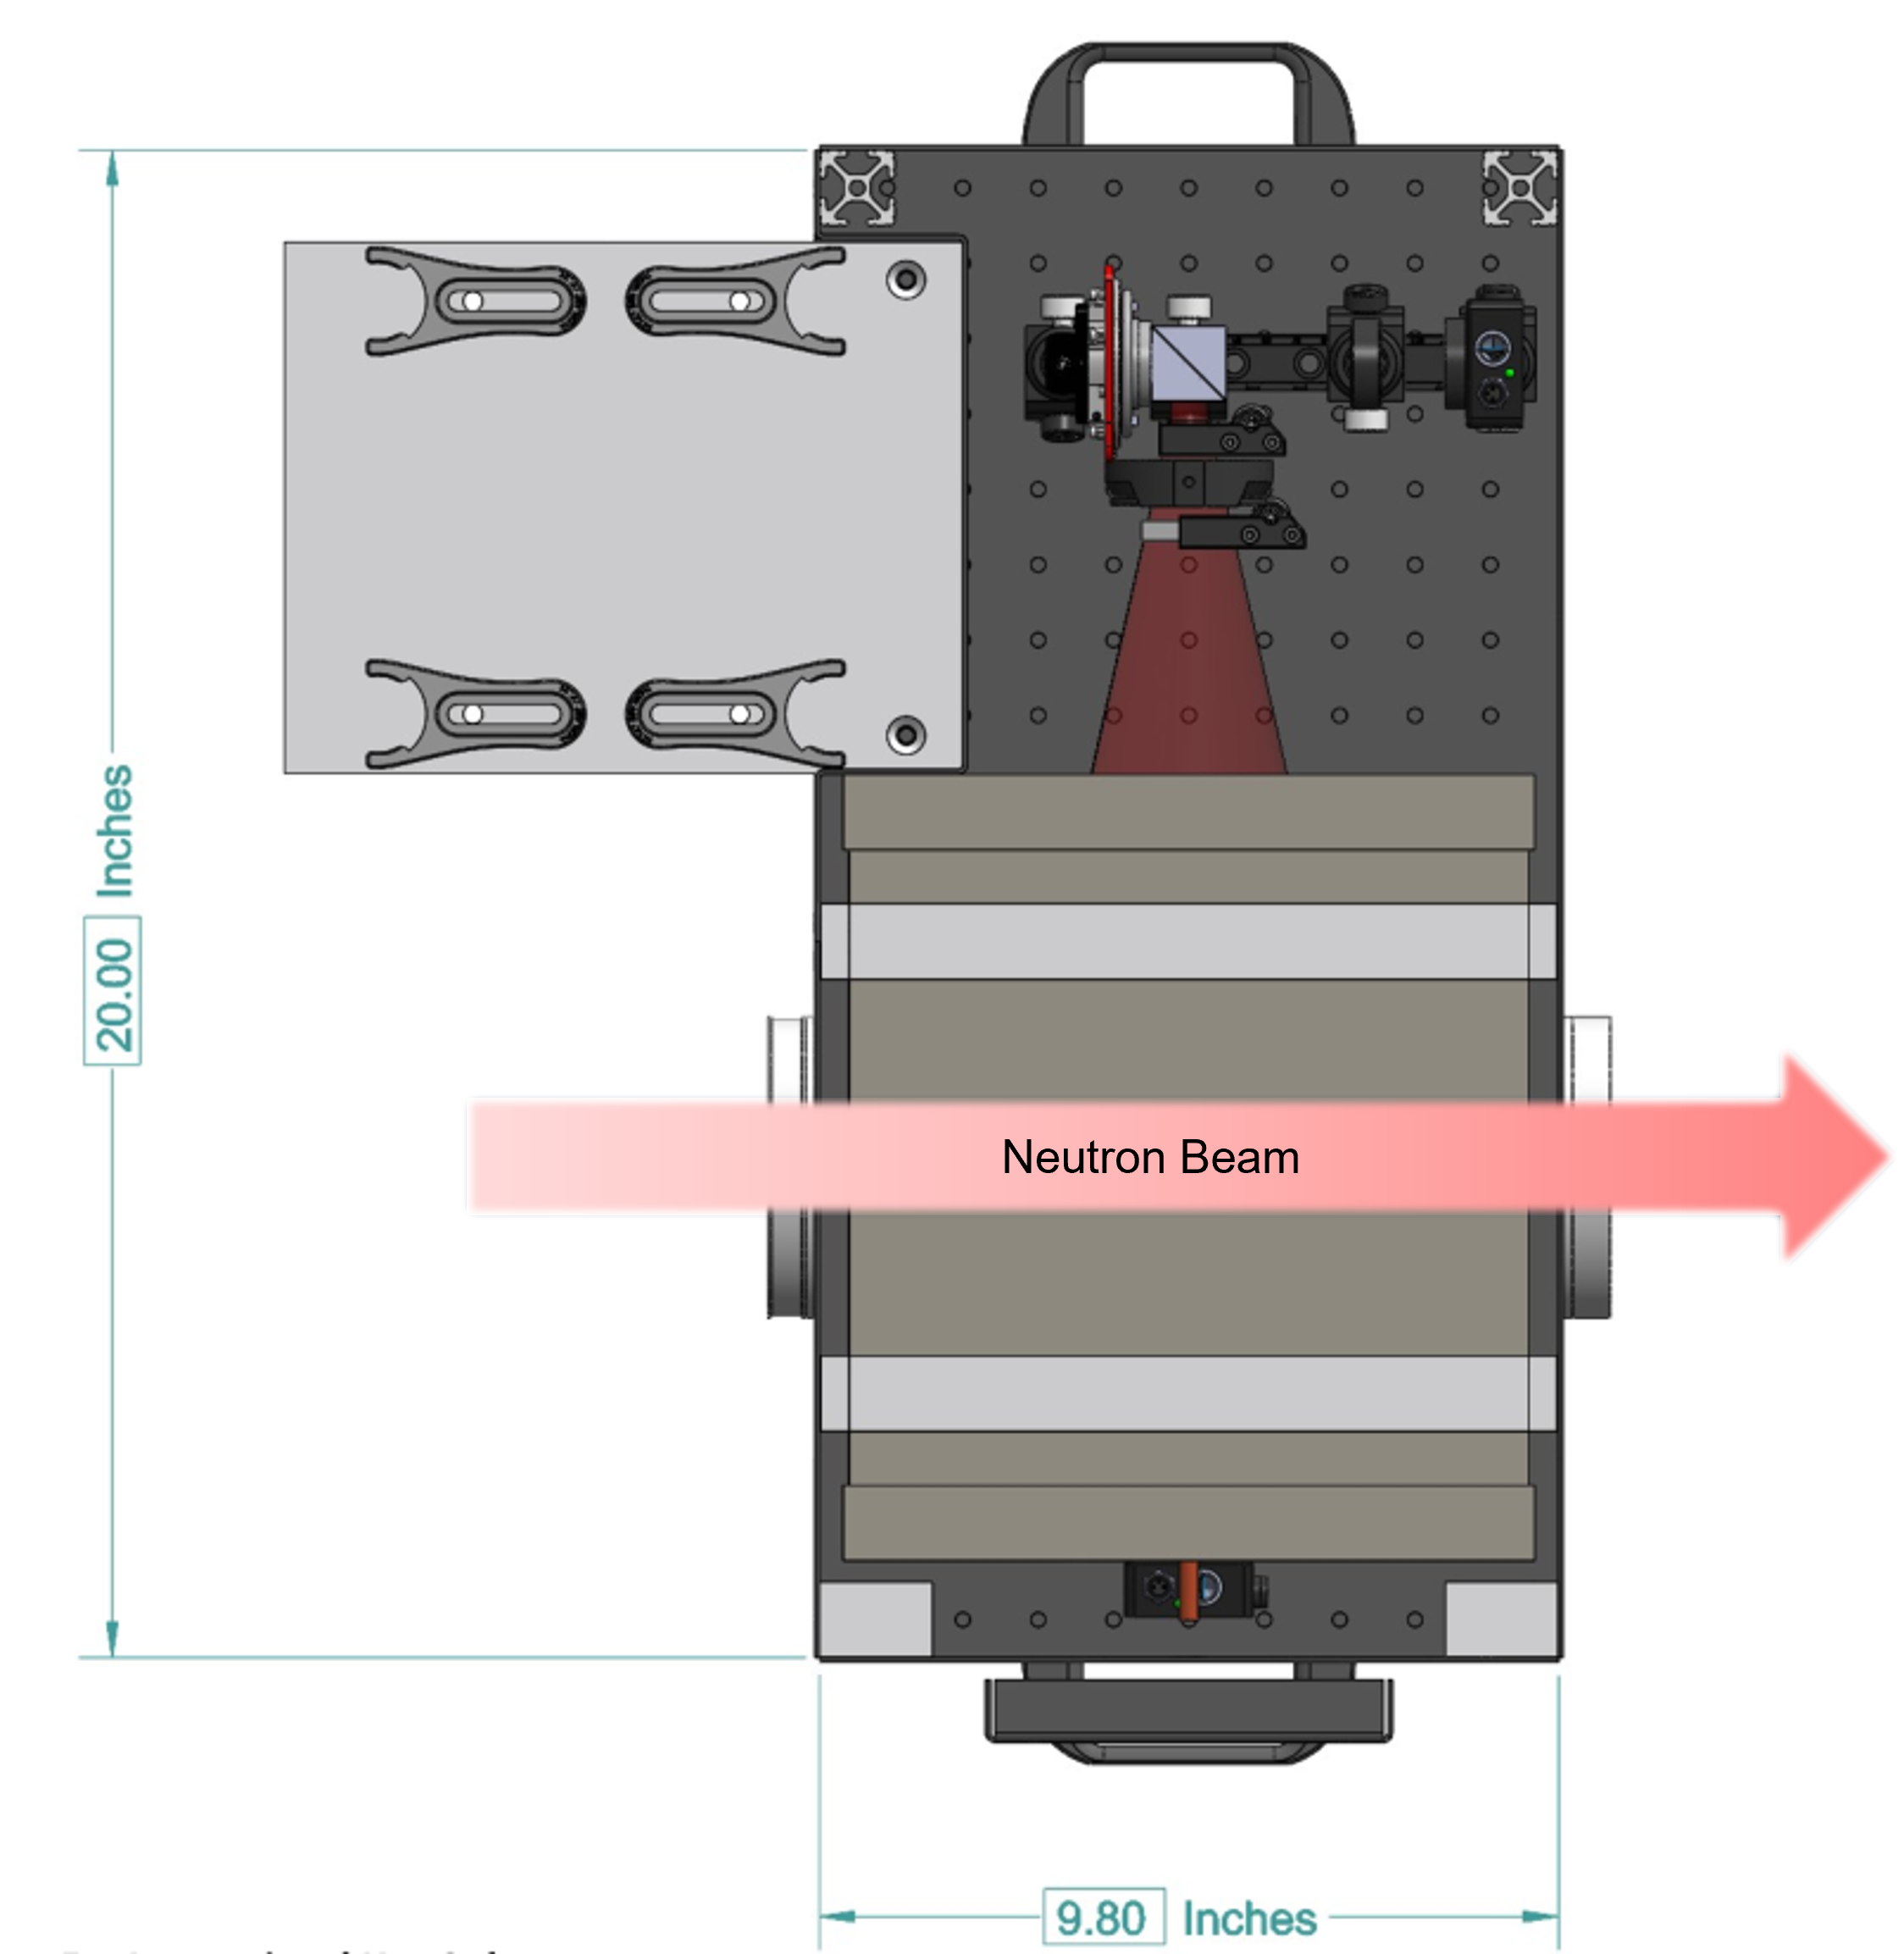
\includegraphics[width=0.8\textwidth, height=0.45\textheight]{figures/chapter3-figs/insitumodel_topdown.png}
         \caption{Top down view.}
         \label{fig:insitu_topdown}
     \end{subfigure}

    \caption{A CAD model of the in situ SEOP system with the major components highlighted.}
    \label{fig:insitumodel}
\end{figure}
\clearpage}

\afterpage{
\begin{figure}
    \centering
    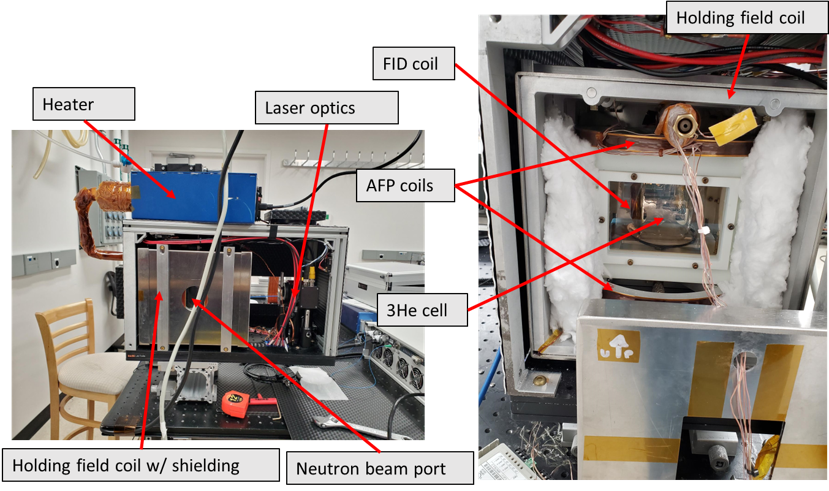
\includegraphics[width=\textwidth]{figures/chapter3-figs/insitupic.png}
    \caption{The in situ $^3$He polarization SEOP system built for the neutron polarimetry experiment conducted in this thesis.}
    \label{fig:insitupic}
\end{figure}
\clearpage}

\subsection{Cell Production}

The $^3$He cell used for this experiment is named “Soccer”. Soccer is made of aluminosilicate glass, GE180, as per the benefits mentioned earlier in this chapter. Soccer has an outer diameter of 7.58 cm and an outer length of 6.62cm. Soccer is placed inside the oven of the in situ SEOP system such that the neutron beam goes along the length of the cell, as illustrated in \cref{fig:insitumodel} and \cref{fig:insitupic}. Soccer was made by the ORNL's glass blowing workshop from GE180 stock. The cell was then installed on the SNS $^3$He filling station \cite{Jiang2013}. It was filled with 0.8bar of $^3$He and 0.08 bar of N$_2$ at room temperature, making it ideal for long wavelength neutron beam polarization measurements. Soccer was built as a hybrid cell with a mixture of Rb and K.

\afterpage{
\begin{figure}
    \centering
    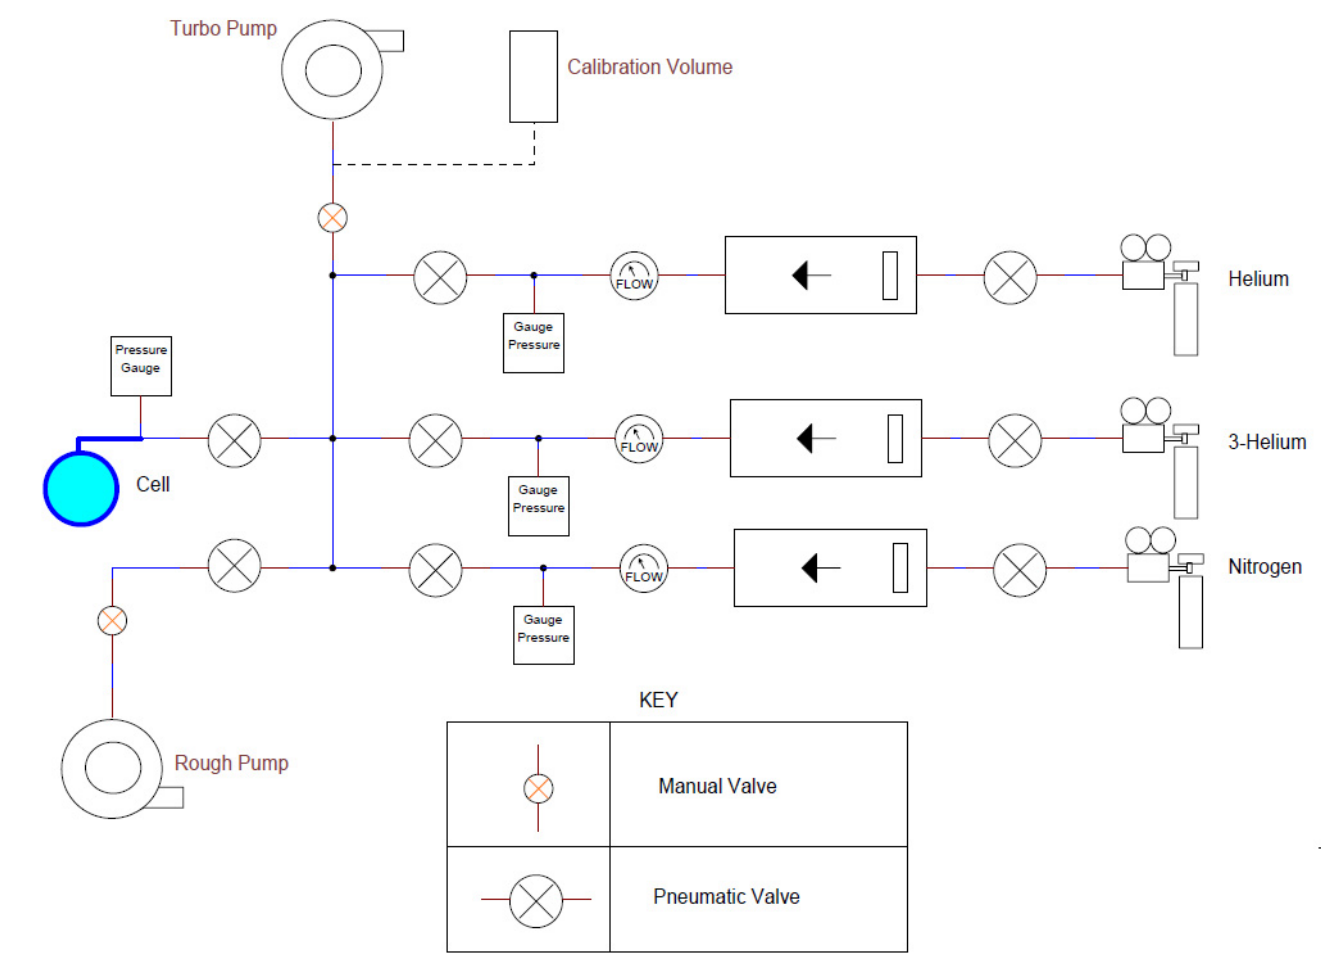
\includegraphics[width=\textwidth]{figures/chapter3-figs/3Hefillingstation.png}
    \caption[Schematic of the SNS $^3$He cell filling station.]{Schematic of the SNS $^3$He cell filling station. Figure taken from \cite{Jiang2013}}
    \label{fig:fillingstation}
\end{figure}
\clearpage}

The glass cell filling is based on the recipe developed by the $^3$He polarization group at National Institute of Standards and Technology (NIST) \cite{Chen2011}. For the first key step, a new cell is thoroughly cleaned prior to filling in order to remove impurities, which can cause a breakdown of SEOP \cite{Chen2011, Jiang2013}. The glass cell stringer assembly is attached to the filling station, as shown in  \cref{fig:fillingstation}, and alkali capsules are dropped into the end tubes, which are then sealed off. The cell is baked at 400 \degree C for two days. A turbo pump is used to pump on the baking cell until high vacuum ($ \sim 10^{-9}$ Torr) is reached. The mass spectrum from Residual Gas Analyzer is also monitored. The key during bake off is to remove any residual water content. After baking, the alkali metals in the capsules are boiled using a flame torch and slowly driven into the cell volume. The alkali mixture ratio is very important for hybrid SEOP as explained earlier in this chapter. A white light halogen lamp and a spectrometer are used to measure the relative intensity of the alkali D1 and D2 absorption lines to characterize the alkali mixture desired ratio. NIST has found the ratio of 1/7 to 1/20 for [Rb]/[K] to be ideal for high $^3$He density hybrid SEOP cells \cite{Chen2011}. Soccer was filled with a 1 part Rb to 3 part K ratio because of its low $^3$He density.

After the alkali filling, the cell gets filled with $^3$He and N$_2$. The gas filling takes place with the filling station shown in \cref{fig:fillingstation}. It consists of a N$_2$ line, a ultra high purity (99.999\%) $^3$He line. The cells are filled with N$_2$ first and then $^3$He. After filling, the cell is closed off from the filling station and separated using a flame torch around the stem of the cell to the stringer assembly. Care is taken to ensure no air leaks in during separation. The pressure in the stringer is recorded using the pressure gauges prior to tip off. Using a calibrated volume, the volume of the new cell is obtained. Thus, the final $^3$He pressure in the cell at room temperature is determined using the ideal gas law. The true cell pressure is determined later from neutron attenuation measurements.

\subsection{Magnetostatic Cavity}

\afterpage{
\begin{figure}
    \centering
    \begin{subfigure}[c]{0.75\textwidth}
        \centering
         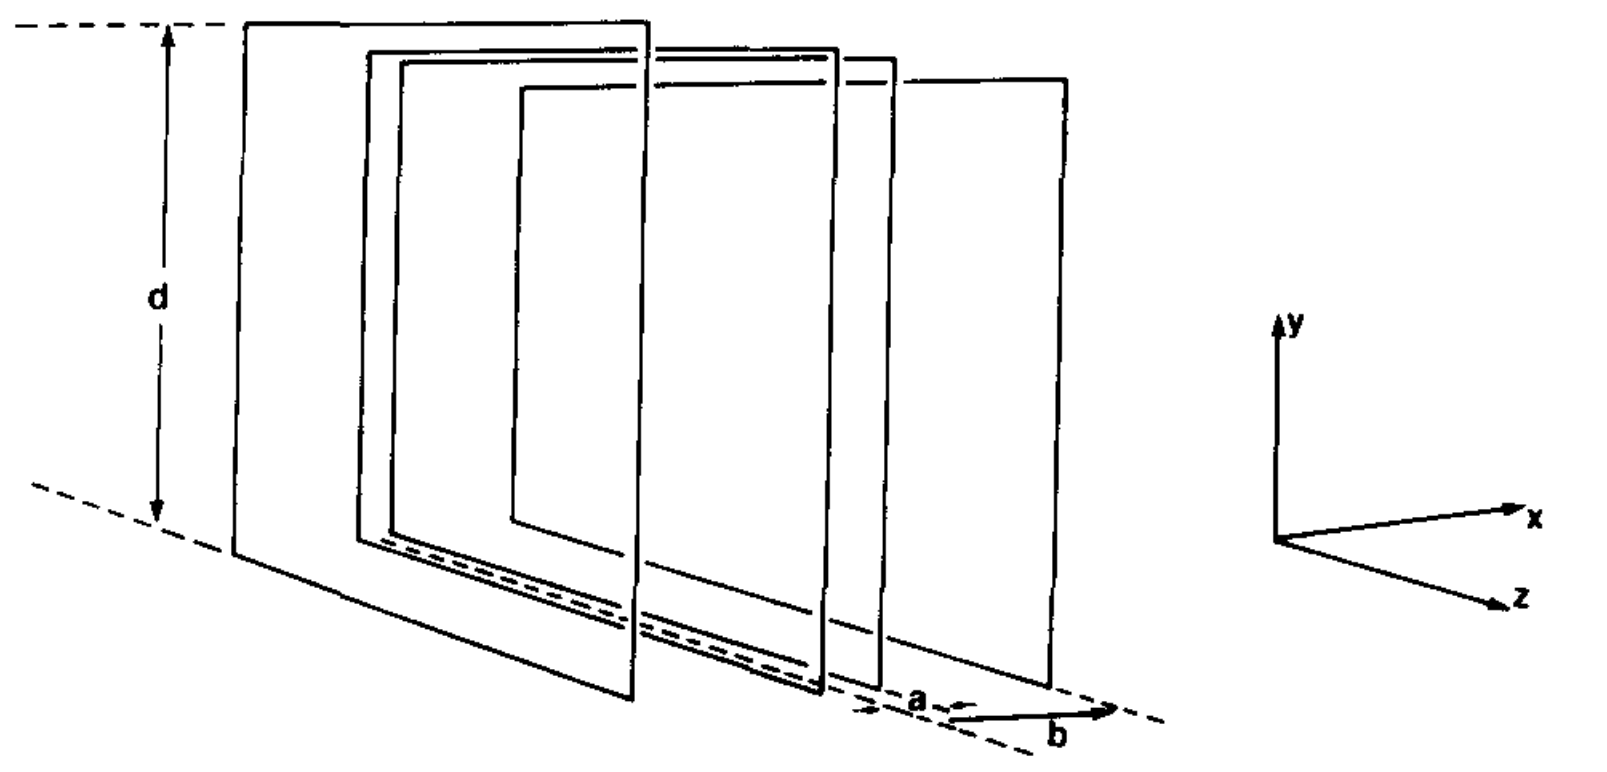
\includegraphics[width=\textwidth]{figures/chapter3-figs/MerrittCoilSchematic.png}
         \caption{A schematic of the four-coil system.}
         \label{fig:Merrittscheme}
     \end{subfigure}
     \hfill
     \begin{subfigure}[c]{0.5\textwidth}
        \centering
         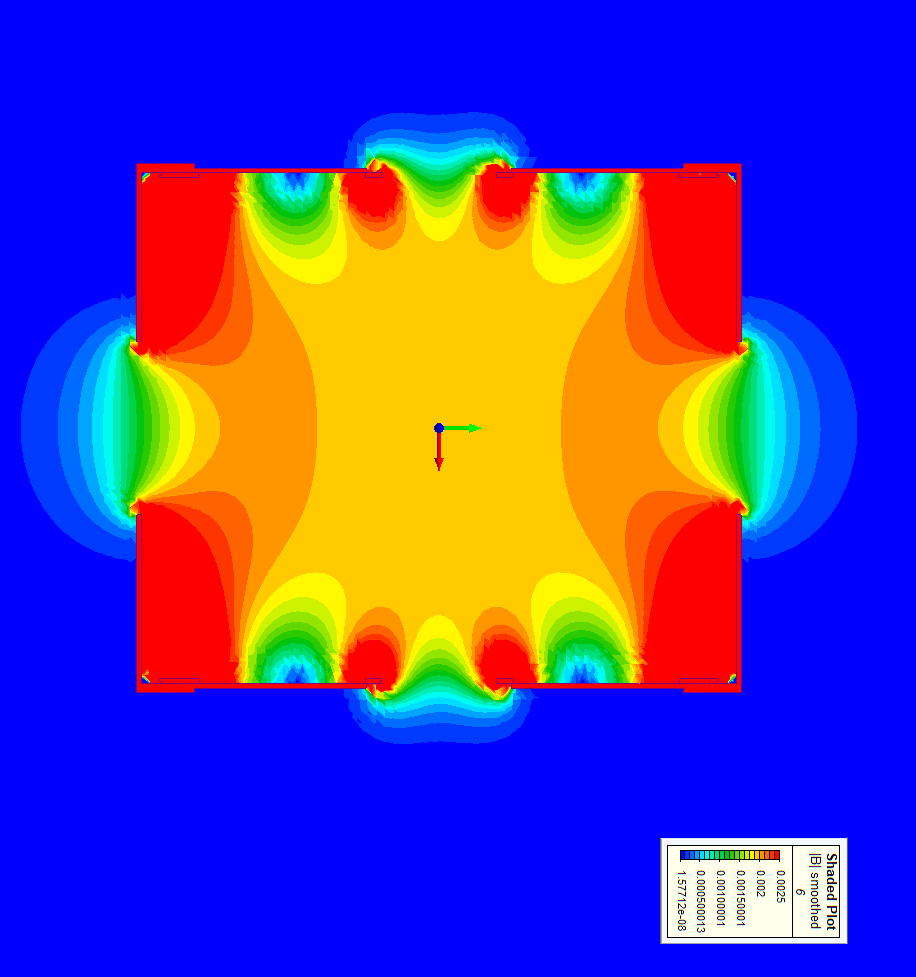
\includegraphics[width=\textwidth]{figures/chapter3-figs/insitumerrittcoil_gradient.png}
         \caption{Simulated magnetic field profile of the four-coil system.}
         \label{fig:Merrittfield}
     \end{subfigure}

    \caption[Merritt's four-coil geometry]{Merritt's four-coil geometry proposed in \cite{Merritt1983}. (b) shows the finite element simulations of the magnetic field profile produced by the 4-coil geometry of the in situ system.}
    \label{fig:Merritt}
\end{figure}
\clearpage}

As described earlier, the $^3$He cell needs to operate in a magnetic holding field in order to define a reference for the polarization. This holding magnetic field also must satisfy the low magnetic fields gradient requirements to prevent $^3$He relaxation. In the in situ system, the holding magnetic field is provided by the four-square coil configuration proposed in \cite{Merritt1983}, a schematic of which is shown in \cref{fig:Merrittscheme}. This four square coil geometry creates a uniform magnetic field for the cell by satisfying:
\begin{itemize}
    \item ratio of the distance, $a$, from the center of the four coils to the inner pair of coils and, $d$, the side length of the coils as $\frac{a}{d} = 0.128$ \cite{Merritt1983}.
    \item ratio of the distance, $b$, from the center to the outer pair of coils and, $d$, as $\frac{b}{d} = 0.505$ \cite{Merritt1983}.
    \item ratio of the current in the inner coil pair, $I_{in}$, to that in the outer coil pair, $I_{out}$, is $\frac{I_{in}}{I_{out}} = 0.423$ \cite{Merritt1983}.
\end{itemize}  
Finite element simulations, as shown in \cref{fig:Merrittfield}, were performed to determine the best winding and current configuration to achieve low gradient magnetic field. For further uniformity and shielding from external fields, which can cause polarized $^3$He relaxation, a rectangular mu-metal magnetic shielding box is used to envelope the four-coil system. \Cref{fig:insitumodel} shows the a model of the four coils and the mu-metal shield inside the in situ enclosure. For the in situ system, the coil was wound with 18AWG wire, with 33 loops in each of the outer coils and 14 loops in each of the inner coils. The outer coils were connected in series with each other and powered to 2.4 Amps. The inner coils were also connected in series with each other and powered at 4.5 Amps. When fully powered, the magnitude of holding magnetic field produced by the full four-coil system along its longitudinal axis is 12.7 Gauss.

\subsection{Oven and Heating System}

The $^3$He cell must be heated in order to vaporize the alkali mixture inside the cell to initiate the SEOP process. \Cref{fig:insitumodel} shows the oven of the in situ system to accommodate the cell. The oven is made of Silicon based fiberglass, capable of 220 \degree C. All sides (except the top and bottom) of the oven have a fused silica windows, which are transparent to neutrons as well as the laser light. The cell is heated by compressed air coming from a heater, flowing in to the oven chamber via an inlet. The cell sits on a pedestal in the center of the oven.

The heater is operated via a PID controller which allows for monitoring and controlling of the heater’s steady state operation. The heater uses incoming compressed air from the facility at 50 psi and heats it with a 1000 W resistive cable, coupled with a flow feedback switch to ensure air flow. Oven temperature is monitored via two thermocouple sensors, one mounted directly on the oven wall. 

\subsection{Laser and Optics}

The laser selected for in situ $^3$He SEOP system is a 50 W 770 nm narrowband laser with a spectral linewidth of 0.2 nm for the D1 transition pumping of K. The laser operates at 47.5 Amp current and the internal laser diode and variable bragg grating are kept cool using a coolant based chiller. Laser head mounts directly to the in situ system as as shown in \Cref{fig:insitumodel}. In order to optically pump the cell, the high-powered infrared light needs to be circularly polarized to match the D1 line of the alkali. This is done by the laser light going through a series of light polarizing optical components. These are shown in \cref{fig:lasersetup}. 

As shown in \cref{fig:lasersetup}, a rotatable half-wave plate (HWP) and polarizing beam splitter (PBS) are used to linearly polarize and reflect the laser beam. The laser beam emerging from the laser head typically has an 80\% linear polarization. By optimizing the half-wave plate rotation, the maximum intensity of the linearly polarized (s-polarized) light is reflected towards the $^3$He cell by the PBS, while the low intensity (p-polarized) transmitted light is dumped into a light diffuser. The half wave plate optimization at low laser power is shown in \cref{fig:HWP}. This optimization was performed by placing a power meter in place of the diffuser and measuring the incident power as a function of half wave plate rotation. The figure shows that the maximum laser was reflected at 70$\degree$ rotation. This half-wave plate setting ensures that the maximum intensity of polarized laser light is incident on the $^3$He cell as well as the liquid crystal retarder. 

The Liquid Crystal Retarder (LCR), acting like a quarter-wave plate, circularly polarizes the incoming linearly polarized laser beam. The LCR works by applying a voltage through the liquid crystal to alter the birefringence and hence inducing a polarization phase shift to circularly polarize the light. The LCR voltage was tuned to induce both the left-handed ($\sigma_-$) and right-handed ($\sigma_+$) circularly polarized light by measuring the laser polarization using an optical polarimeter. The best possible degree of circular polarization, 80.3\% ($\sigma_-$) and 82.6\% ($\sigma_+$), observed at LCR voltage settings, 3.13 V for ($\sigma_-$) and 2.17 V ($\sigma_+$), respectively, is shown in \cref{tab:docp}. These LCR settings were used during the SEOP operation, 3.13V for polarizing $^3$He parallel to the holding magnetic field and 2.17V for polarizing $^3$He antiparallel to the holding magnetic field. Both the half wave plate and the LCR can be tuned remotely.

\afterpage{
\begin{figure}
    \centering
    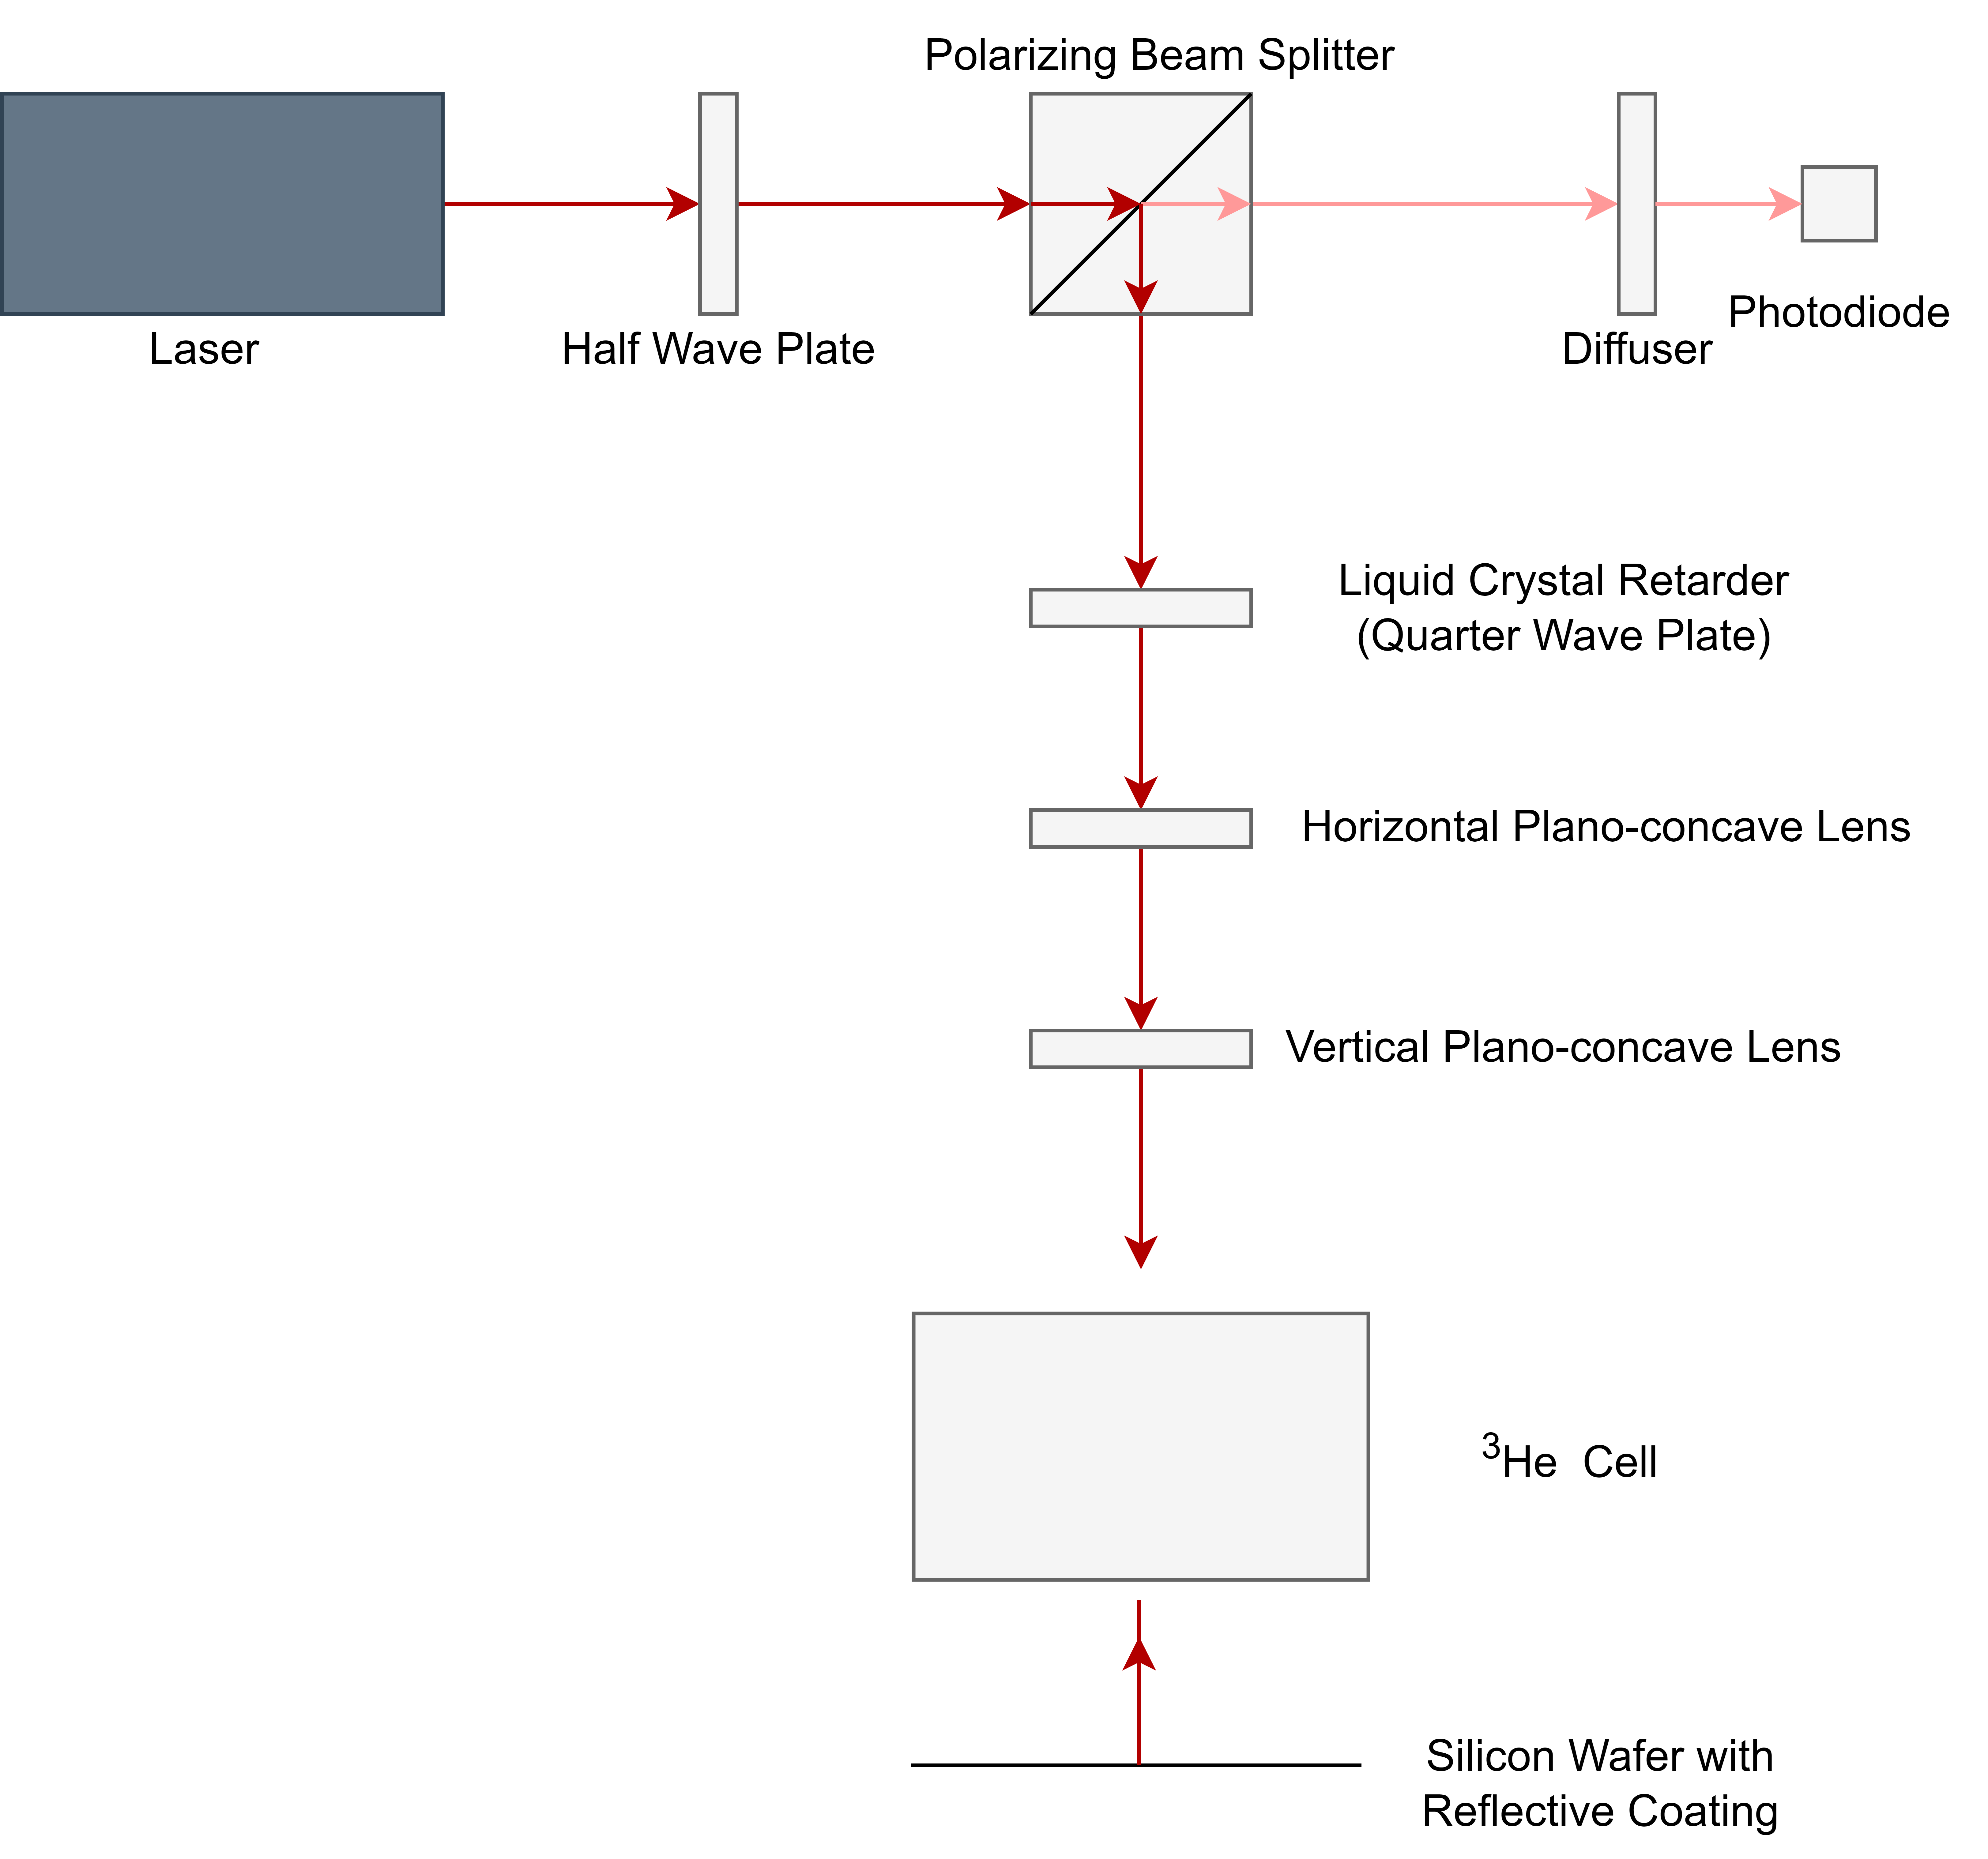
\includegraphics[width=\textwidth]{figures/chapter3-figs/In-situSEOPlaser.png}
    \caption{Setup of the laser optics used in the in situ SEOP system.}
    \label{fig:lasersetup}
\end{figure}
\clearpage}

\afterpage{
\begin{figure}
    \centering
    \includegraphics[width=\textwidth]{figures/chapter3-figs/HWPoptimization.png}
    \caption{Optimization of the half wave plate at 5 A laser power. The trend shows the change in transmitted power as a function of the rotation of the HWP i.e. it's birefringence.}
    \label{fig:HWP}
\end{figure}
\clearpage}

\afterpage{ 

\begin{table}
\centering
\centering
\begin{threeparttable}
\caption{Measured degree of circular polarization of the laser from the liquid crystal retarder acting as a quarter wave plate.}
\label{tab:docp}
\begin{tabular}{@{}cccc@{}}
\toprule
LCR Voltage [V] & Circularly Polarized Light Orientation & DOCP\tnote{*} & DOLP\tnote{**} \\
\midrule
2.17 & Left & 80.47\% & 3.58\% \\
3.13 & Right & 82.17\% & 4.28\% \\
\bottomrule
\end{tabular}

    \begin{tablenotes}
      \item[*] Degree of Circular Polarization
      \item[**] Degree of Linear Polarization
    \end{tablenotes}

  \end{threeparttable}
\end{table}

\clearpage}

The circularly polarized light goes through a series of vertical and horizontal plano-concave lenses to expand the beam spot size so that the entire $^3$He cell is illuminated. An Infrared light sensitive laser phosphor card was used to ensure the full coverage of the cell by the laser light. Even though the laser beam is being applied from oneside to keep the system as compact as possible, a silicon wafer with a reflective coating was placed behind the cell to get double sided laser illumination on the cell.

%\afterpage{
%\begin{figure}
%     \centering
%     \begin{subfigure}{\textwidth}
%         \centering
%         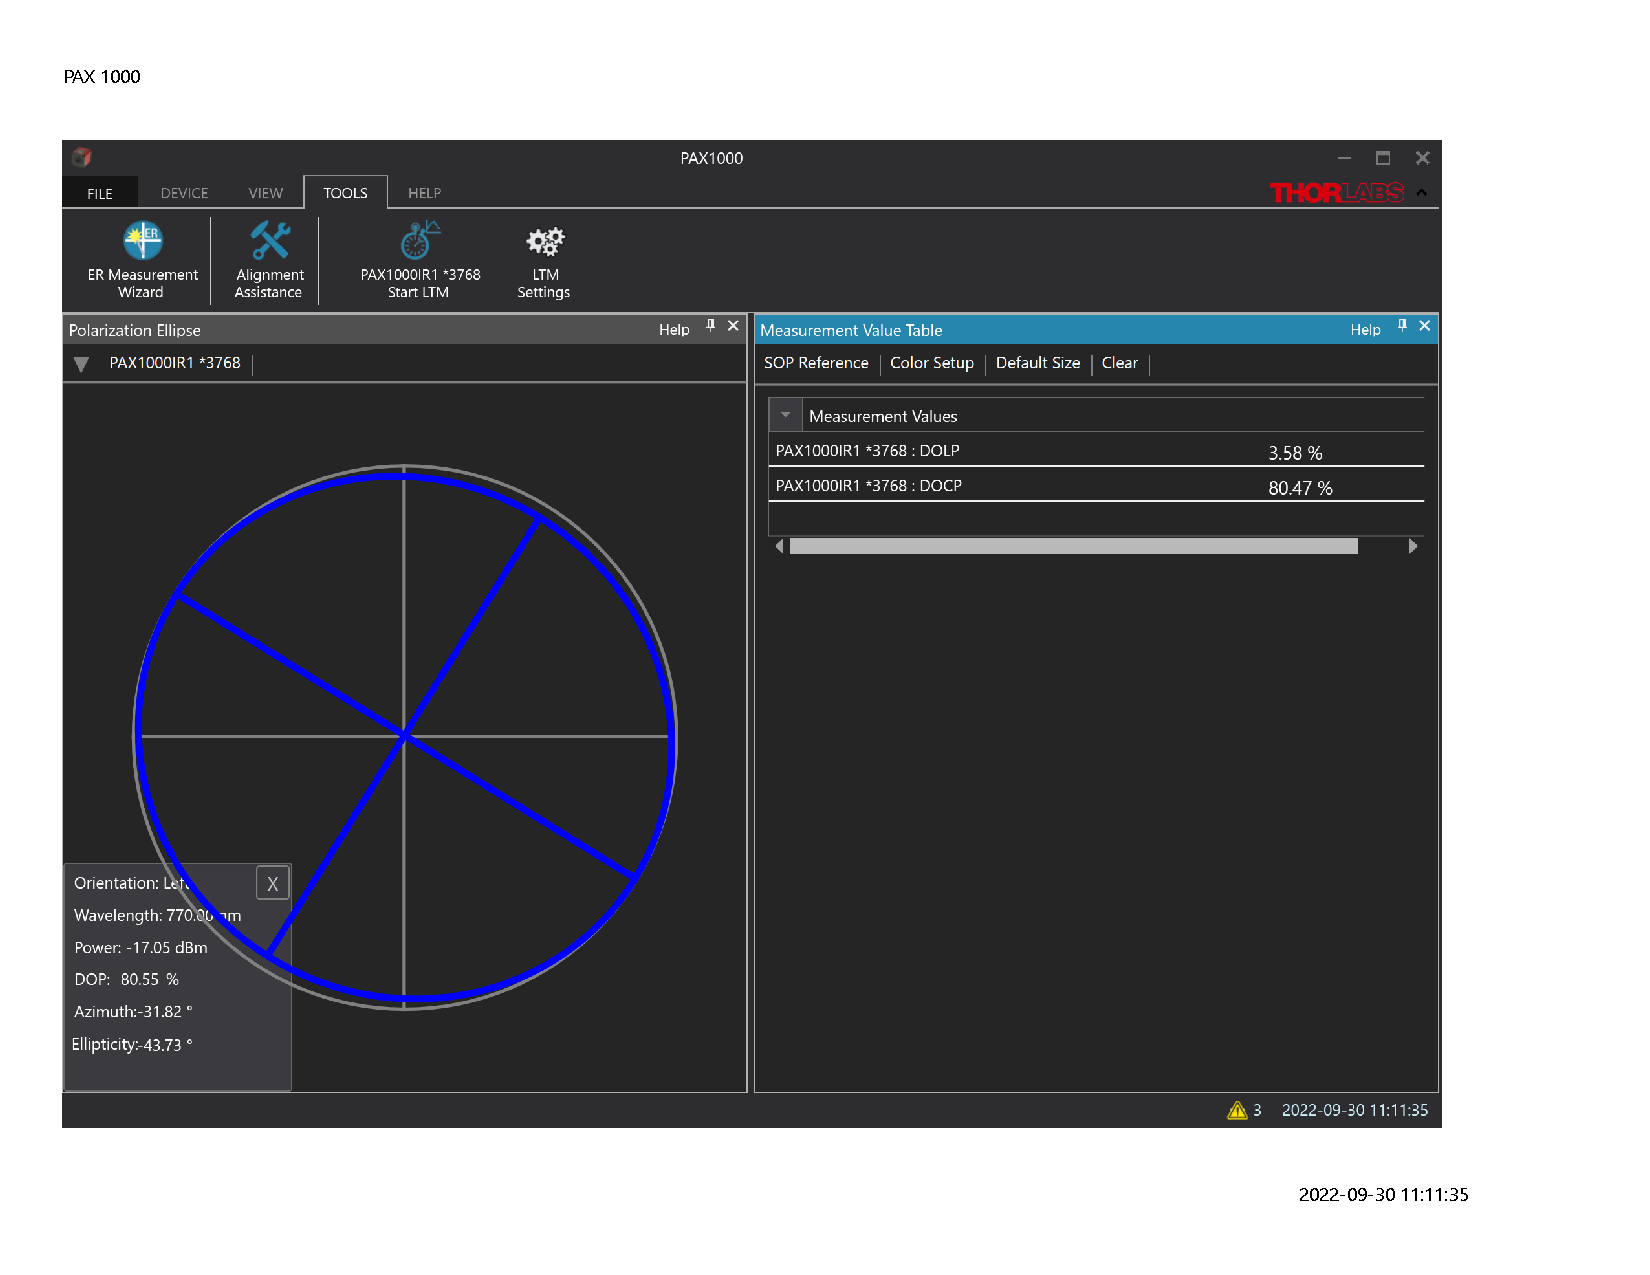
\includegraphics[width=0.7\textwidth]{figures/chapter3-figs/Opt_pol_left.pdf}
%         \caption{Left handed ($\sigma_{-}$) light degree of polarization}
%         \label{fig:leftdop}
%     \end{subfigure}
%     \hfill
%     \begin{subfigure}{\textwidth}
%         \centering
%         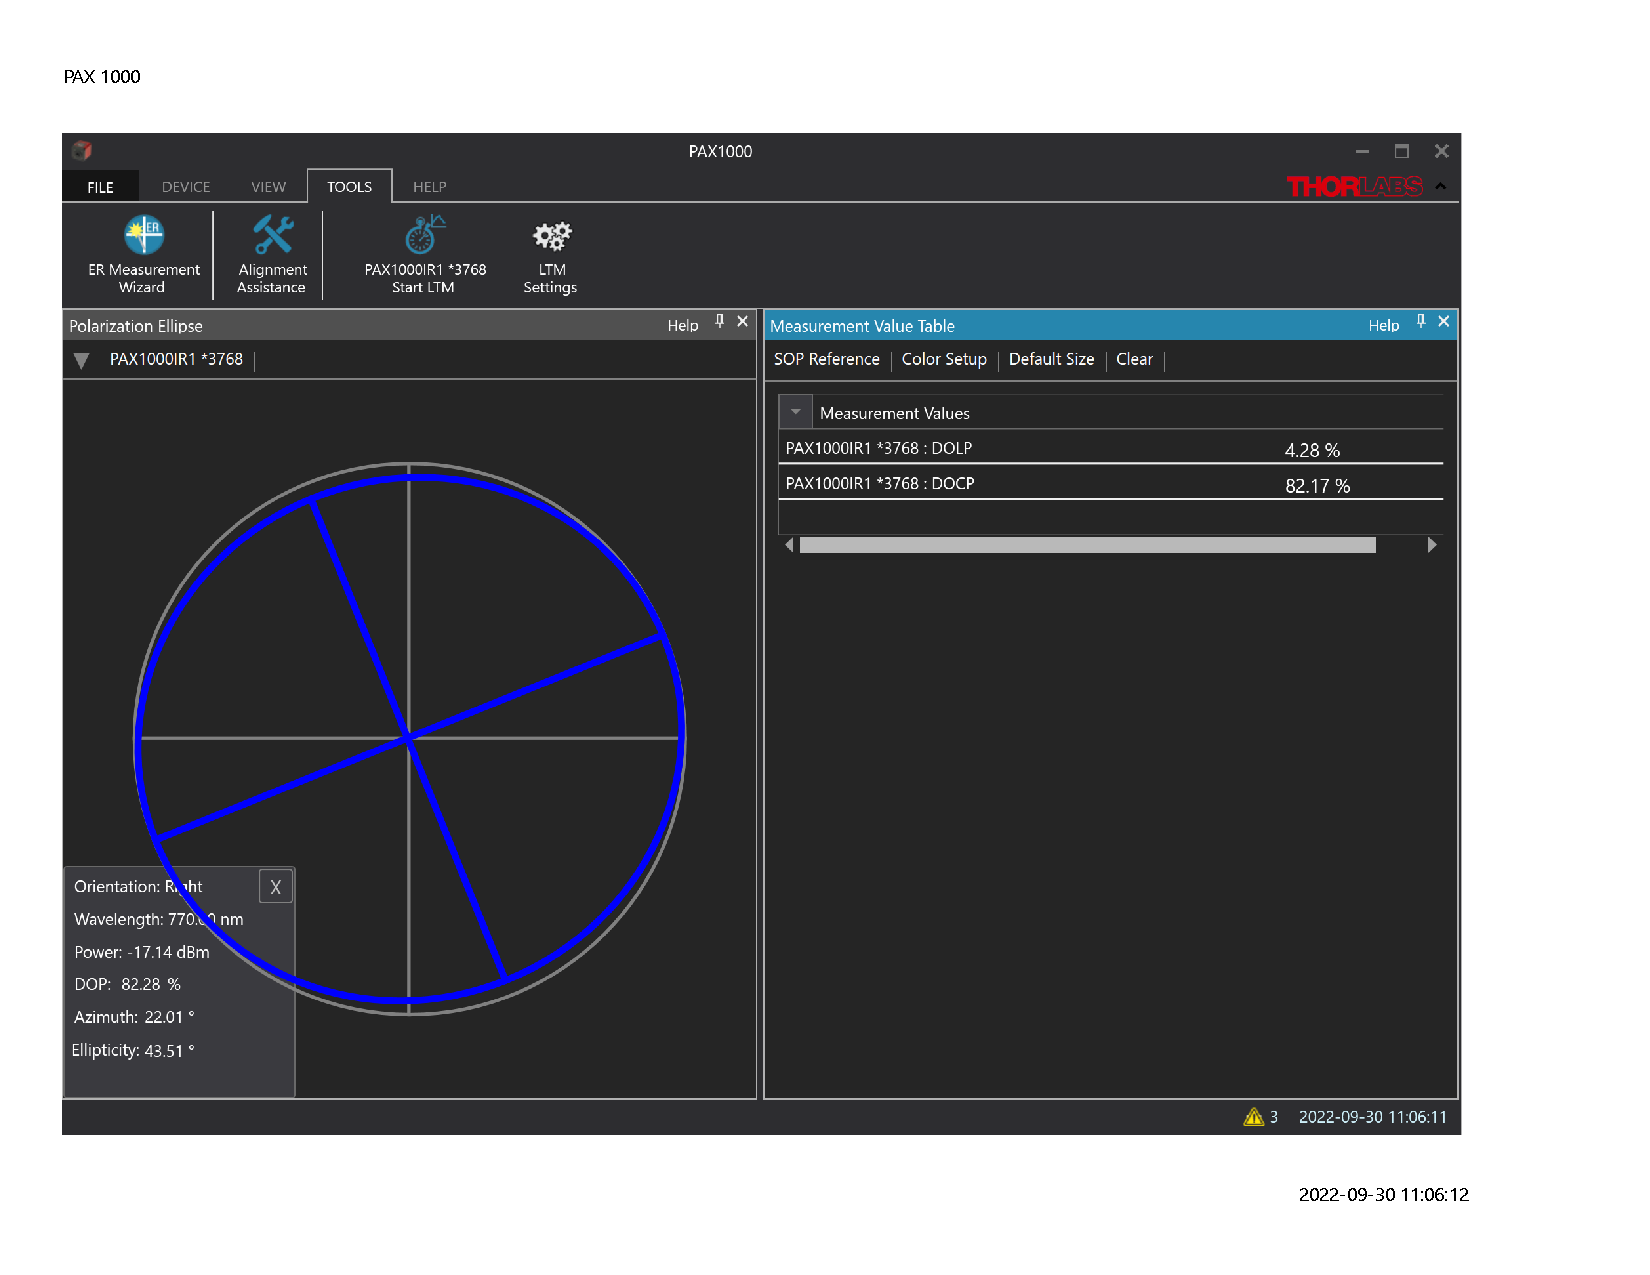
\includegraphics[width=0.7\textwidth]{figures/chapter3-figs/Opt_pol_right.pdf}
%         \caption{Right handed ($\sigma_{+}$) light degree of polarization}
%         \label{fig:rightdop}
%     \end{subfigure}
%        
%        \caption{Measured degree of circular polarization of the laser from the liquid crystal retarder acting as a quarter wave plate.}
%        \label{fig:docp}
%
%\end{figure}
%\clearpage}

Since the in situ system was to be operated at a beamline and not a designated laser laboratory, the laser must operate as a Class 4 embedded Class 1 configuration to comply with the safety guidelines of the SNS. The in situ system laser was interlocked with the side enclosure panels using limit switches. Tampering of the enclosure during laser operations would trigger the limit switches and the laser would be de-energized instantly. This feature ensures the safety of the personnel working in close proximity to the in situ system under a fault scenario. This feature also simplified the experimental setup, by eliminating the need for light tight barriers/curtains and laser safety PPE.


\section{Characterization and Control of $^{3}$He Polarization}

There are three widely used methods to monitor and manipulate the $^3$He polarization of $^3$He cells: Nuclear Magnetic Resonance (NMR) Spectroscopy \cite{Lorenzon1993, Romalis1998}, Electron Paramagnetic Resonance (EPR) Spectroscopy \cite{Romalis1998, Babcock2005} and neutron transmission \cite{Jones2000, Chupp2007}. For the in situ system, an NMR system capable of both Free Induction Decay (FID) and Adiabatic Fast Passage (AFP) techniques as well as an EPR system was built. This section will describe them and their use in performance testing of the in situ system.

\subsection{Nuclear Magnetic Resonance Spectroscopy}

Technically, EPR and neutron transmission provide an absolute measurement of the $^3$He polarization. However, NMR can still be used as diagnostic tool for monitoring/manipulating the $^3$He polarization, spin up time and $T_1$ time as well as to measure the relative magnetic field gradients, albeit only to optimize the magnetic field environment rather than as an absolute magnetometer. This section describes the FID and AFP NMR setup used in the in situ system.

\subsubsection{Free Induction Decay}

The relative $^3$He polarization is typically monitored by FID NMR \cite{Bloch1946, Abragam1961}. In FID NMR, a small pickup coil mounted on the $^3$He cell is used to apply a RF pulse to slightly tip the $^3$He spins off the Larmor precession. Then, the transverse component of the $^3$He precession relaxing back from the tip towards the longitudinal Larmor precession induces a signal in the pick up for detection. This signal shows the relaxing transverse precession as an decaying oscillation envelope characterized by, $T_2^*$, the transverse polarization relaxation time, given as
\begin{equation}
    \frac{1}{T_2^*} = \gamma_3 \Delta B_0
\end{equation}
where $\gamma_3$ is the $^3$He's gyromagnetic ratio and $\Delta B_0$ is presence of gradients over the portion of $^3$He polarization volume sampled by the coil. $T_2^*$ is representative of fluctuations in spin precession from magnetic-field inhomogeneities.

This magnetization measurement approach is mostly nondestructive since small tip angles are used from a pickup coil of size smaller than the cell \cite{Lorenzon1993, Parnell2008, Chen2011}. $T_2^*$ is typically on the order of milliseconds, where longer $T_2^*$ means smaller magnetic field gradients, $\Delta B_0$ \cite{Lorenzon1993,  Parnell2008, Chen2011}.

For the in situ system, the FID coil is a circular coil, about 1 inch in diameter, with 150 loops of 0.0093 inch diameter copper wire, taped to the cell. The total coil resistance is 2.6 $\Omega$. The coil applies a RF pulse of 1.5 ms duration and 10 V amplitude orthogonal to the holding field, $B_0$. The short pulse duration time is necessary for the diabatic field tipping process at the Larmor frequency of 41.16 kHz (12.7 Gauss). Otherwise, the $^3$He spins can get adiabatically locked to the tipping field plus holding magnetic field $B_0+B_{RF}$ and lose their polarization. The tipping magnetic field leads to a transverse component in the polarization, which induces a voltage (FID signal) in the pickup coil at the rising and falling edge of the $B_{RF}$ pulse. The FID signal consists of the falling edge since there is a low chance of inducing a field gradient some time after $B_{RF}$ was applied, resulting in longer $T_2^*$. 

The FID setup is based on the technique by \cite{Parnell2008} and shown in \cref{fig:NMRsetup}. The signal from the pickup coil is fed into a low pass filter with a transmission/reciever switch, with a high quality factor. Pick up coil is only active when the control software requests an FID signal to prevent a self oscillating circuit, which would degrade $^3$He polarization. The signal after the preamplifier gets fed into digital I/O card [National Instruments USB-6259] with a built-in phase lock-in amplifier. NI USB-6251 DAC board also generates reference frequency signal close to the $^3$He Larmor frequency via an internal phase locked loop. This reference frequency is used to determine the phase of the outgoing waveform signal. The reference frequency was set so the beat frequency of the outgoing signal and the reference signal was in the 100-300 Hz range. The frequency bin width is set at 1 $\mu$Hz to prevent aliasing. 

\afterpage{
\begin{figure}
    \centering
    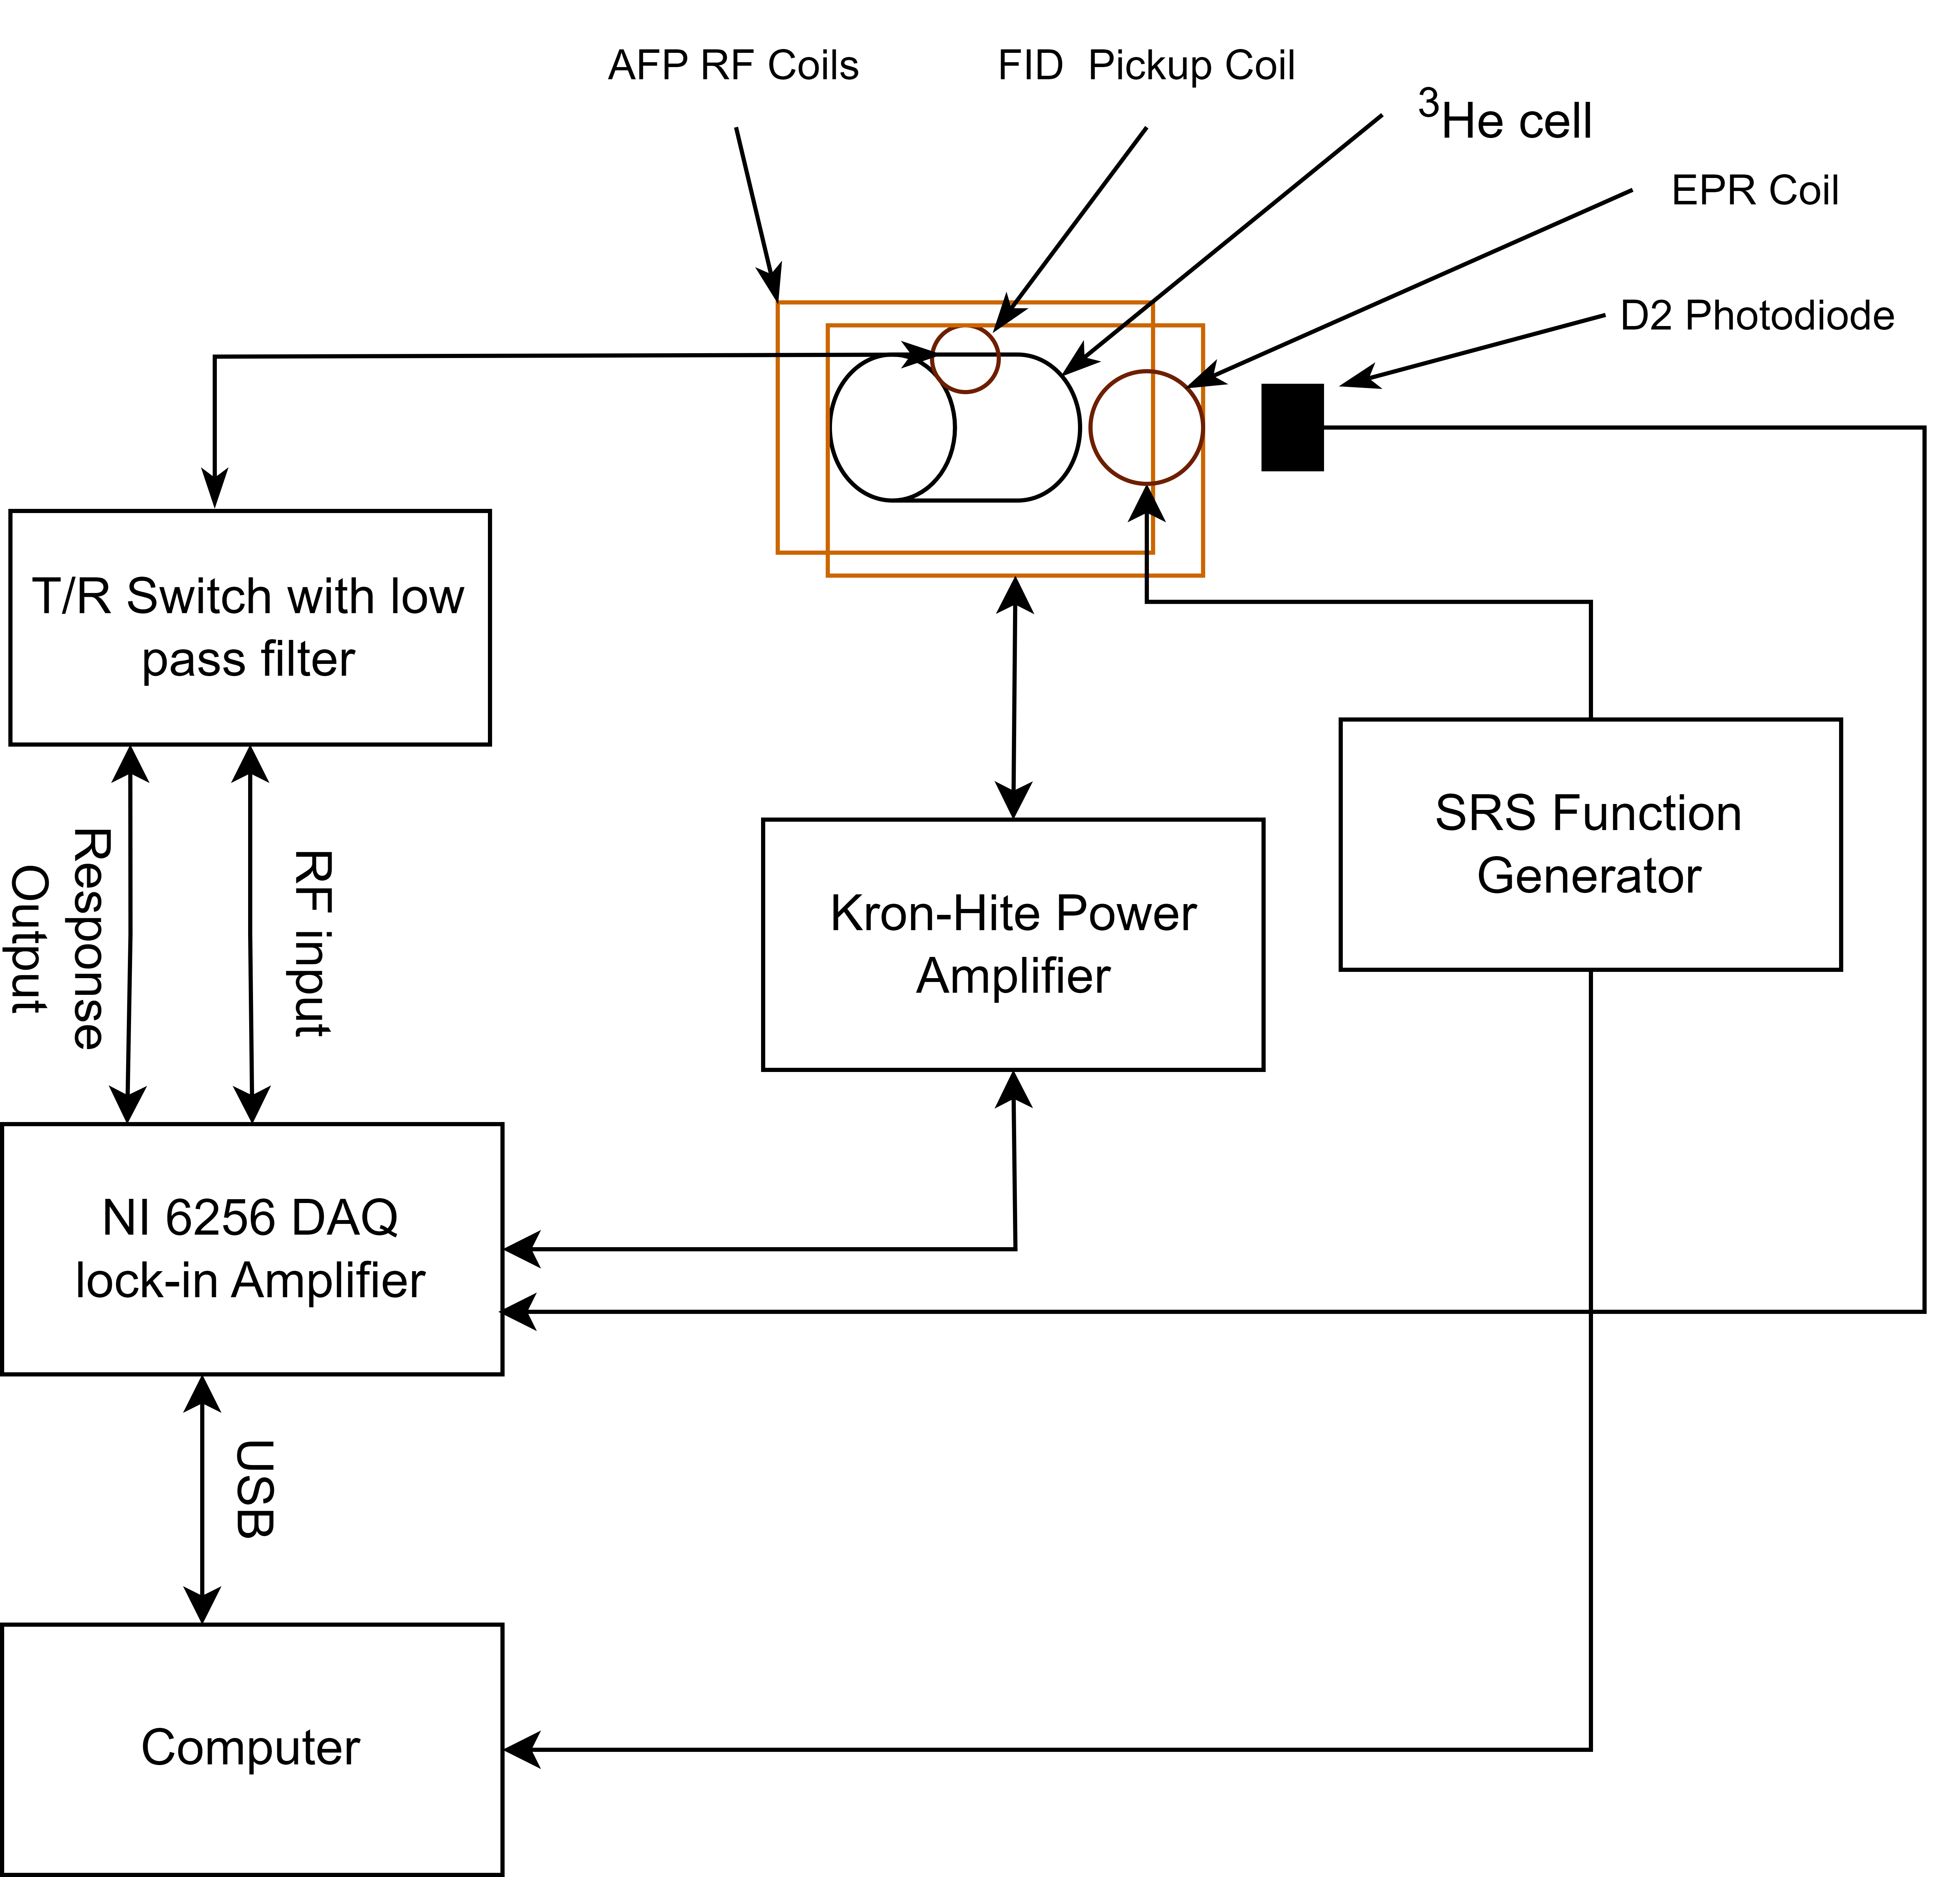
\includegraphics[width=\textwidth]{figures/chapter3-figs/NMRSetup.png}
    \caption[Schematic of the NMR setup used in the in situ SEOP system based on the digitization technique]{Schematic of the NMR setup used in the in-situ SEOP system based on the digitization technique described in \cite{Parnell2008}.}
    \label{fig:NMRsetup}
\end{figure}
\clearpage}

\Cref{tab:FID_params} shows the parameters used to optimize the FID NMR system. \Cref{fig:FIDsignals} shows the raw FID response signal based the parameters in \cref{tab:FID_params}. \Cref{fig:FFTxcomp} and \cref{fig:FIDycomp} shows the decomposed FID signal along with the fit based on: 
\begin{equation}
    f(t) = \frac{1}{2} V_{pp} sin(\omega_L t + \phi) \exp\left( \frac{-t}{T_2^*}    \right)
    \label{eq:FID}
\end{equation}
where $V_{pp}$ is the peak to peak voltage caused by the spin precession tipping from the FID pulse and $\omega_L$ is the Larmor frequency and $\phi$ is the phase of the sinusoidal wave.

\afterpage{
\begin{table}
\centering
\caption{List of parameters used for FID NMR on polarized $^3$He.}
\label{tab:FID_params}
\begin{tabular}{@{}lc@{}}
\toprule
FID Parameters                 & FID Parameter Values \\ 
\midrule
Larmor Frequency {[}Hz{]}      & 41160                \\
Pulse Length {[}sec{]}         & 0.0015               \\ 
RF Amplitude {[}V{]}           & 5-10               \\ 
B-field {[}V{]}                & 2.07               \\ 
Readout Time {[}sec{]}         & 0.08               \\
Additional Mute Time {[}sec{]} & 0.0025               \\
Low pass filter {[}Hz{]}       & 1000               \\
Signal Range {[}V{]}           & 0.1               \\
\bottomrule
\end{tabular}
\end{table}
\clearpage}

\afterpage{
\begin{figure}
    \centering
    \begin{subfigure}[b]{0.5\textwidth}
        \centering
        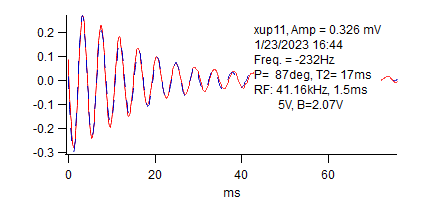
\includegraphics[width=\textwidth]{figures/chapter3-figs/xup_graph.png}
        \caption{x-component of decomposed FID coil response. The units on y-axis are mV.}    
        \label{fig:FFTxcomp}
    \end{subfigure}
    \hfill
    \begin{subfigure}[b]{0.5\textwidth}  
        \centering 
        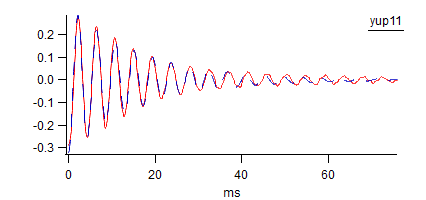
\includegraphics[width=\textwidth]{figures/chapter3-figs/yup_graph.png}
        \caption{y-component of decomposed FID coil response. Notice the 90$\degree$ phase shift with respect to the x-component. The units on y-axis are mV.}    
        \label{fig:FIDycomp}
    \end{subfigure}
    \vskip\baselineskip
    \begin{subfigure}[b]{0.5\textwidth}   
        \centering 
        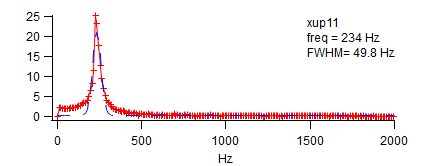
\includegraphics[width=\textwidth]{figures/chapter3-figs/FFT_graph.png}
        \caption{Fast Fourier Transform of the FID coil response.}    
        \label{fig:FIDFFT}
    \end{subfigure}
    \hfill
    \begin{subfigure}[b]{0.5\textwidth}   
        \centering 
        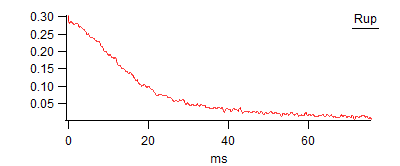
\includegraphics[width=\textwidth]{figures/chapter3-figs/rup_graph.png}
        \caption{A plot of R of FID response. The units on y-axis are mV.}    
        \label{fig:FIDr}
    \end{subfigure}
    \caption{FID response of the polarized $^3$He cell, Soccer. Red curve is the measured response and the blue curve is the fit.}
    \label{fig:FIDsignals}
\end{figure}
\clearpage}

The key indicators from this fit are (i) $T_2^*$ time, which can be used monitor any variations in magnetic field inhomogeneities over time, (ii) the signal amplitude in [mV], which is used to monitor the relative change in $^3$He polarization over time, and (iii) the phase, which can be used to check for polarization inversion by for e.g. as AFP flip or any dephasing due to magnetic field gradients. \cref{fig:FIDFFT} shows the FFT spectrum of the FID response signal. The spectrum peak represents the beat frequency of the larmor precession of the $^3$He polarization and with respect to the reference frequency set by the lock-in amplifier. FFT spectrum can be used to check for sudden or unwanted changes the holding magnetic field, $B_0$. The integral of the FFT spectrum is also proportional to the $^3$He cell polarization, so if the absolute $^3$He polarization is well known, then the integral of the FFT can be used to monitor any changes in absolute $^3$He polarization. In NMR, response signal can be affected by what is known as radiation damping, where different precessions can generate a RF induced current in the coil causing the FID response to be damped \cite{Augustine2002}. It can also happen if the induced FID signal becomes in resonance with the coil. \Cref{fig:FIDr} shows that $R=\sqrt{(x^2 + y^2)}$, where x is the x-comp of FID and y is the y-comp of FID. R in addition to the FFT spectrum can be used to monitor any damping of the FID signal from noise.

\Cref{fig:NMRLoss} shows that the application of a FID pulse sequence results in a relative $^3$He polarization loss of 1-cos($\theta$) = 0.33\% per 5 pulses, corresponding to a tipping angle of $\theta \approx 4\degree$. Due to minimal losses in $^3$He polarization from FID, this NMR monitoring can be utilized in parallel with neutron beam transmission data taking. Even though only a comparative $^3$He polarization is extracted by the FID method, nevertheless, it is useful for monitoring the polarization buildup saturation time as well as the polarization decay ($T_1$ time) i.e lifetime of the $^3$He cell. In \Cref{fig:spinup}, the characteristic time of the fit exponential is called the "spin up time" i.e. the time it takes for $\frac{1}{e}$ population of $^3$He to polarize. The curve plateaus off as time indicating $^3$He cell polarization saturation. For an in situ system, because the $^3$He cell is undergoing continuous optical pumping, this curve should saturate as function of time. In \Cref{fig:spindown}, the characteristic time of this exponential is called the "spin down time" or the $T_1$ time i.e. the time it takes for $\frac{1}{e}$ population of $^3$He to depolarize. Although this time is irrelevant for in situ SEOP systems, courtesy of continuous in situ SEOP polarization, nevertheless, it showcases the longevity of a $^3$He cell polarization in a holding magnetic field.

\afterpage{
\begin{figure}
    \centering
    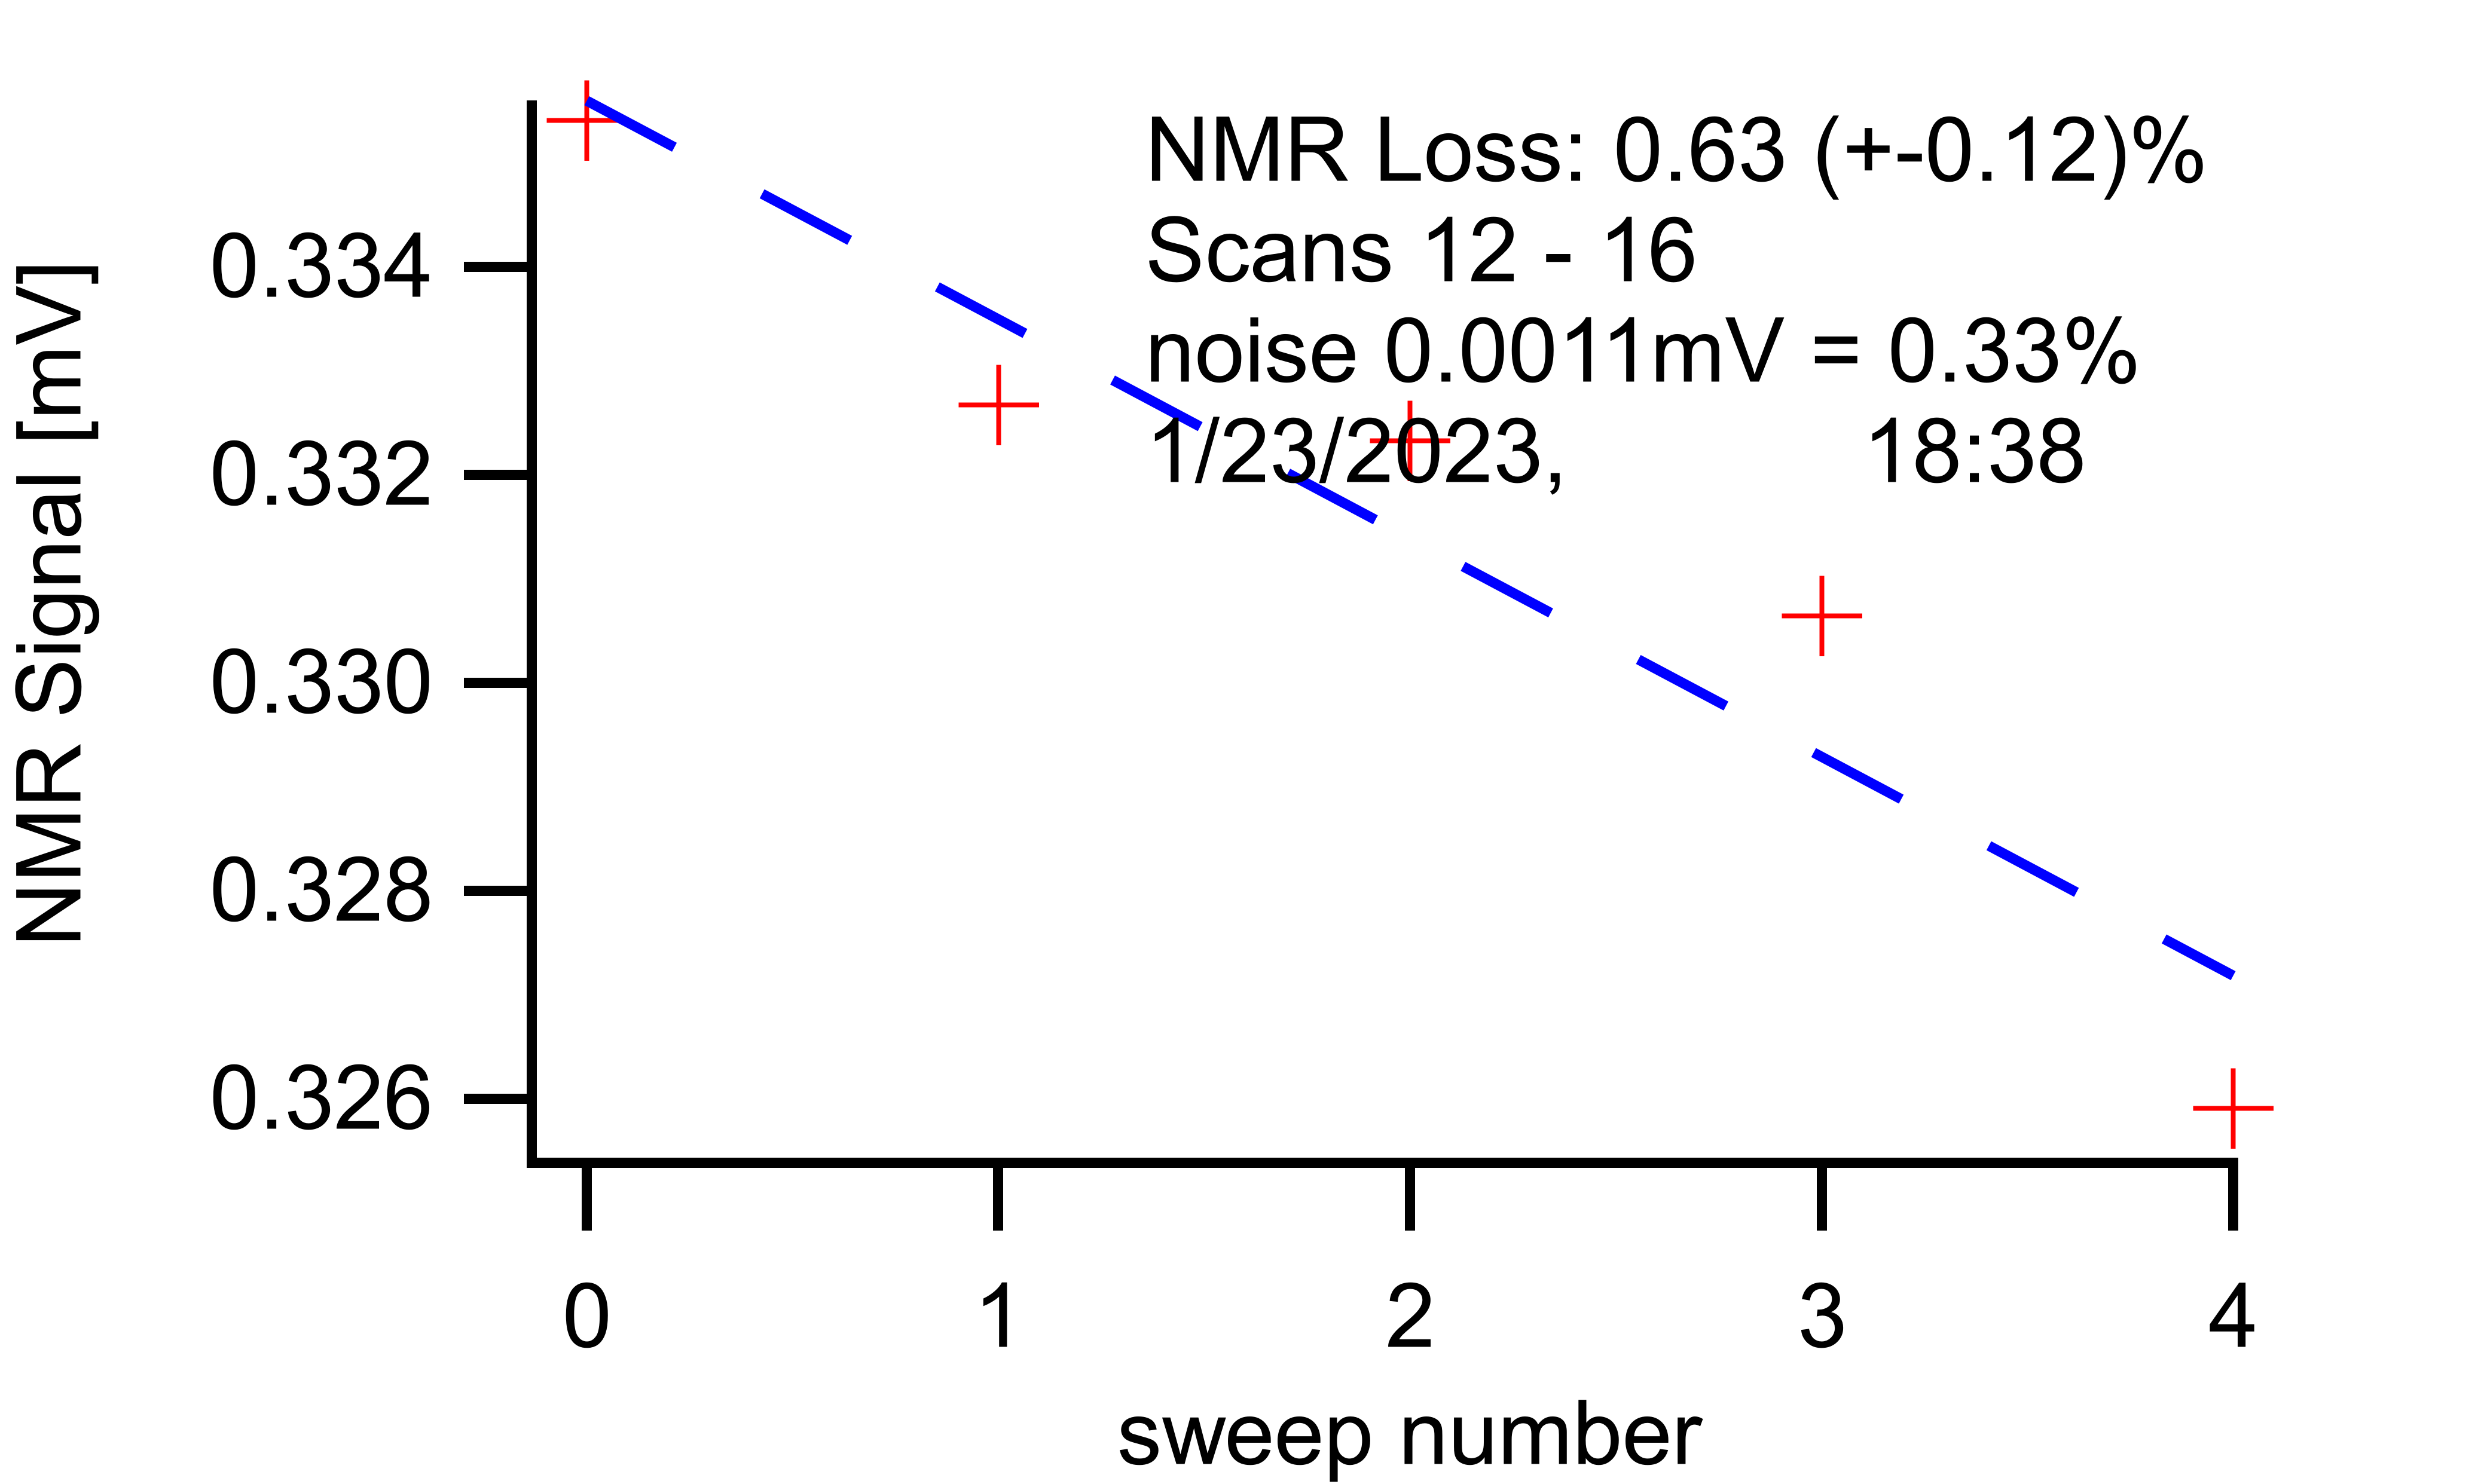
\includegraphics[width=\textwidth]{figures/chapter3-figs/NMRLoss_graph.png}
    \caption{Measured loss in FID response signal after 5 consecutive FID measurements. FID response is in red and the fit is the blue curve. }
    \label{fig:NMRLoss}
\end{figure}
\clearpage}

\afterpage{
\begin{figure}
    \centering
    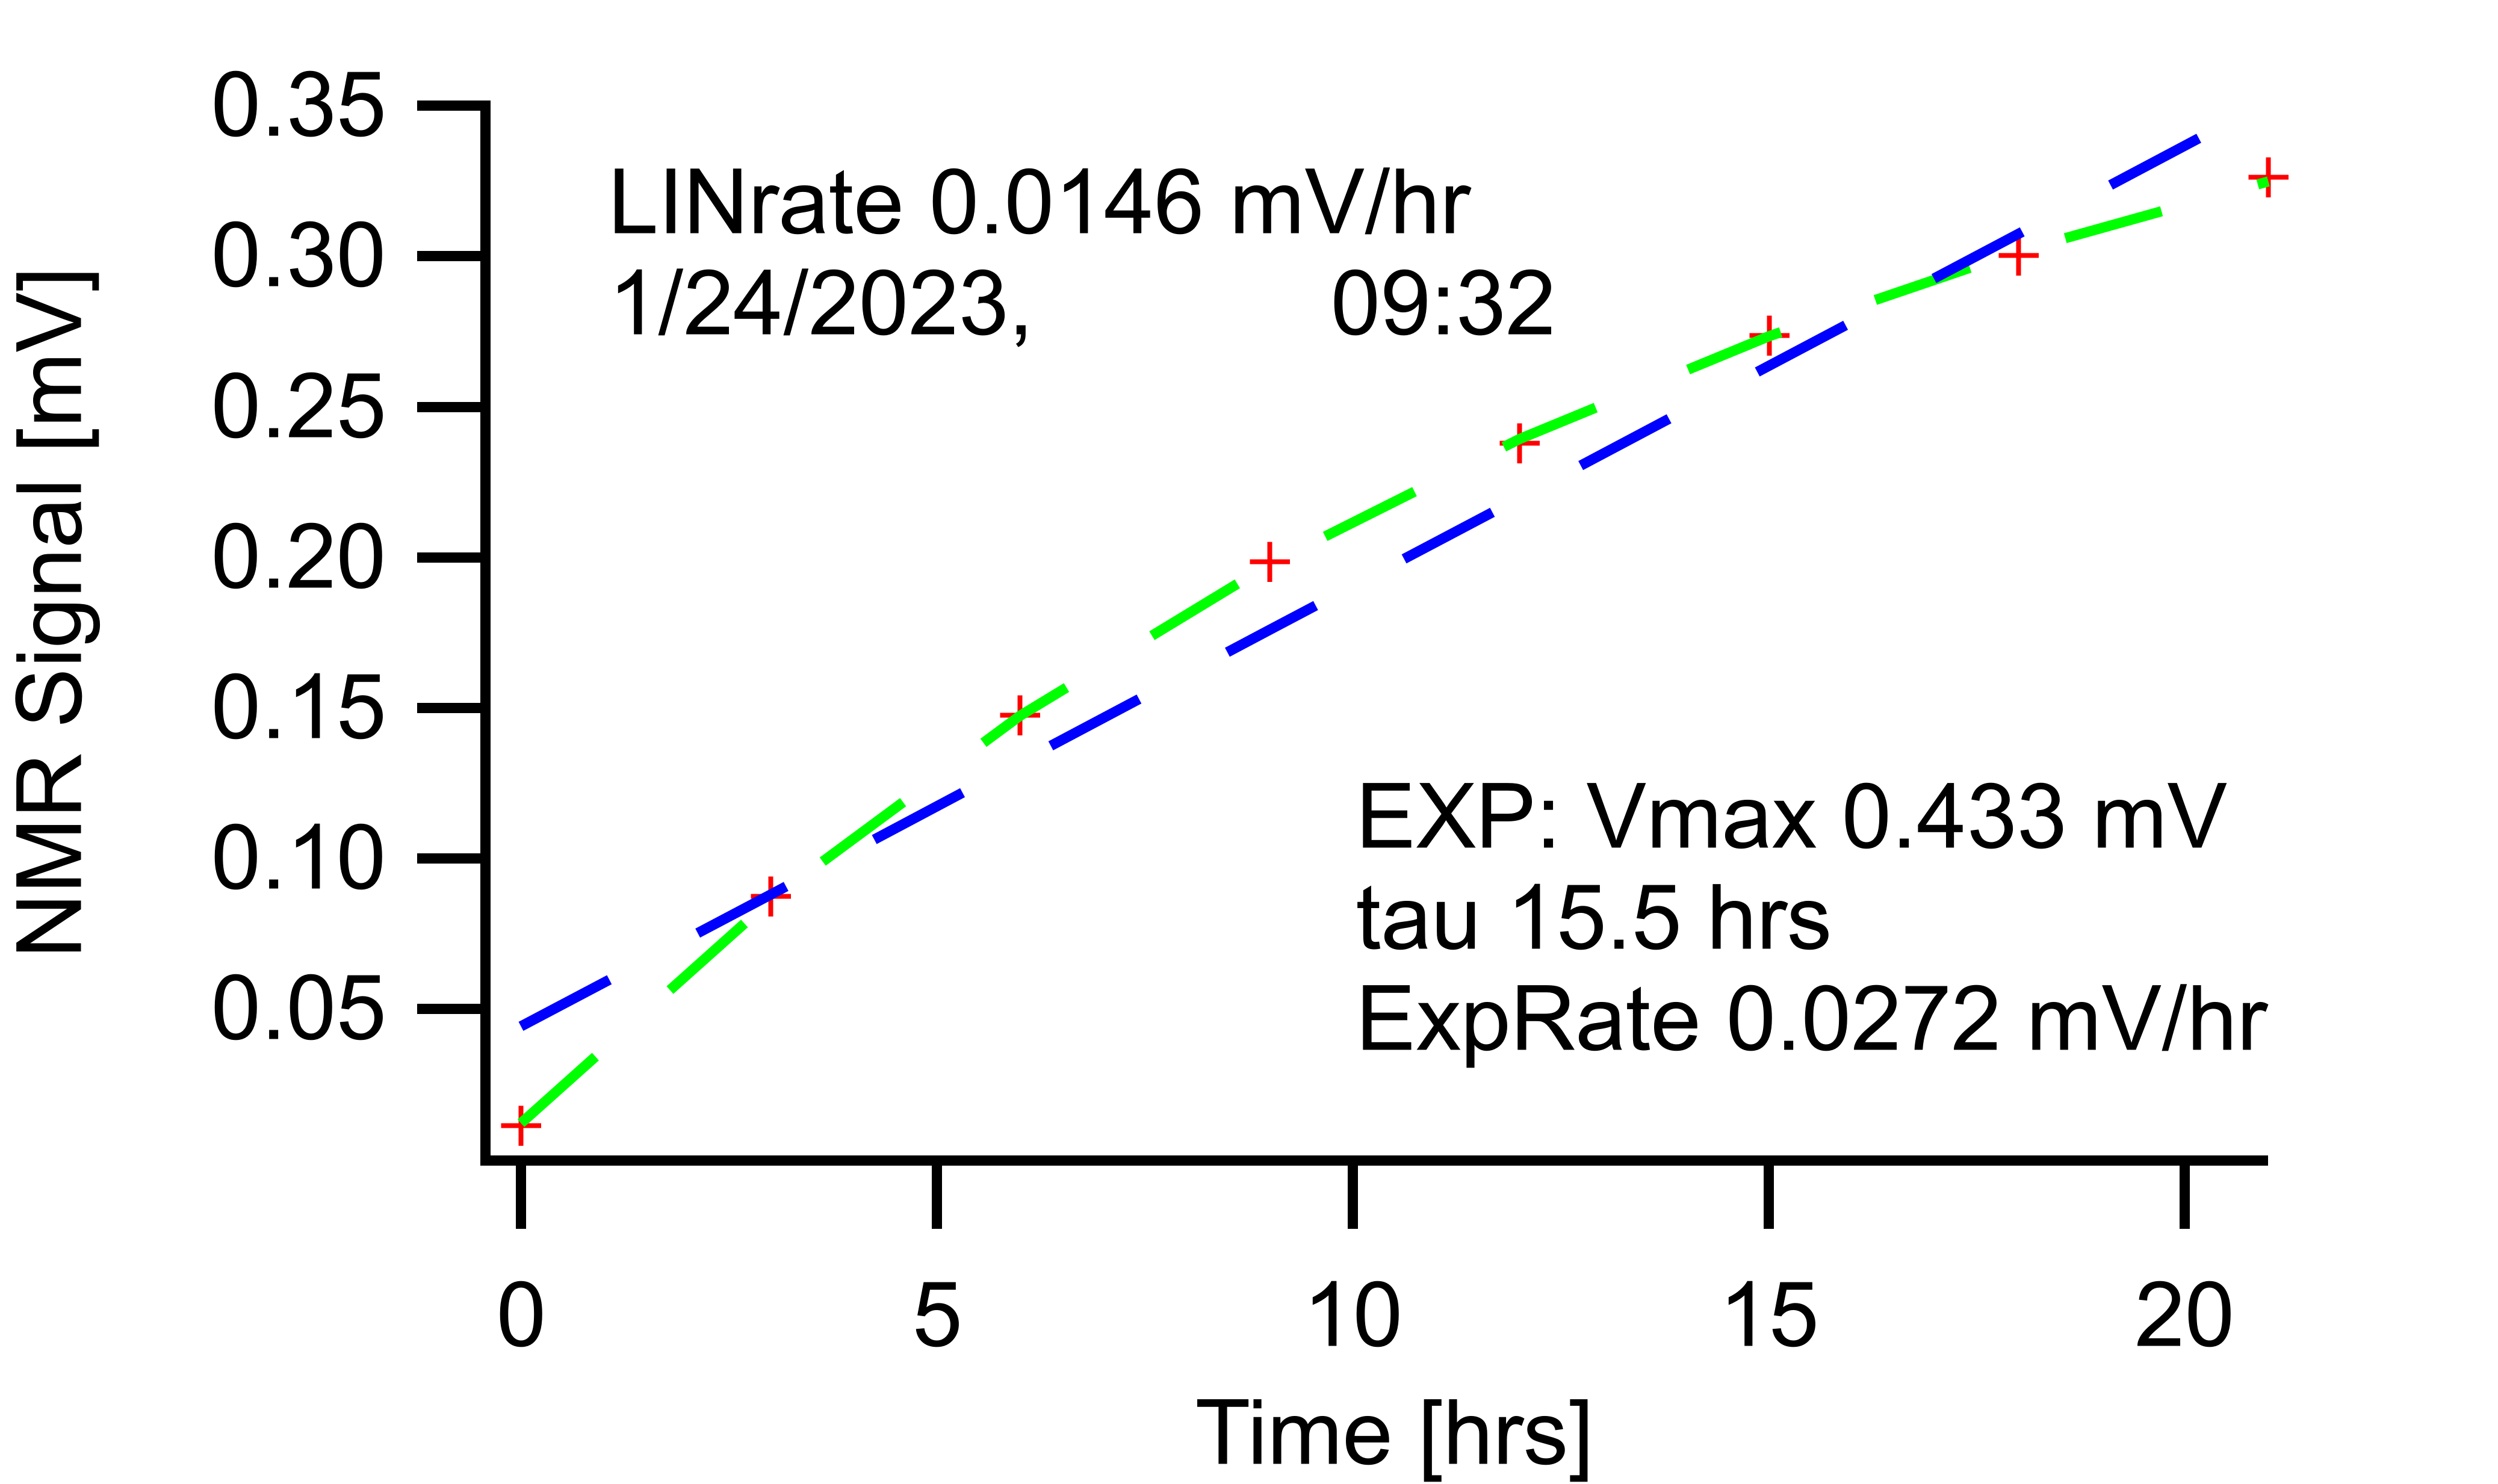
\includegraphics[width=\textwidth]{figures/chapter3-figs/Rate_graph.png}
    \caption{Response of the FID from the $^3$He over a course of time during the SEOP operation. The red points are the measured value and the green curve is the exponential growth fit.}
    \label{fig:spinup}
\end{figure}
\clearpage}

\afterpage{
\begin{figure}
    \centering
    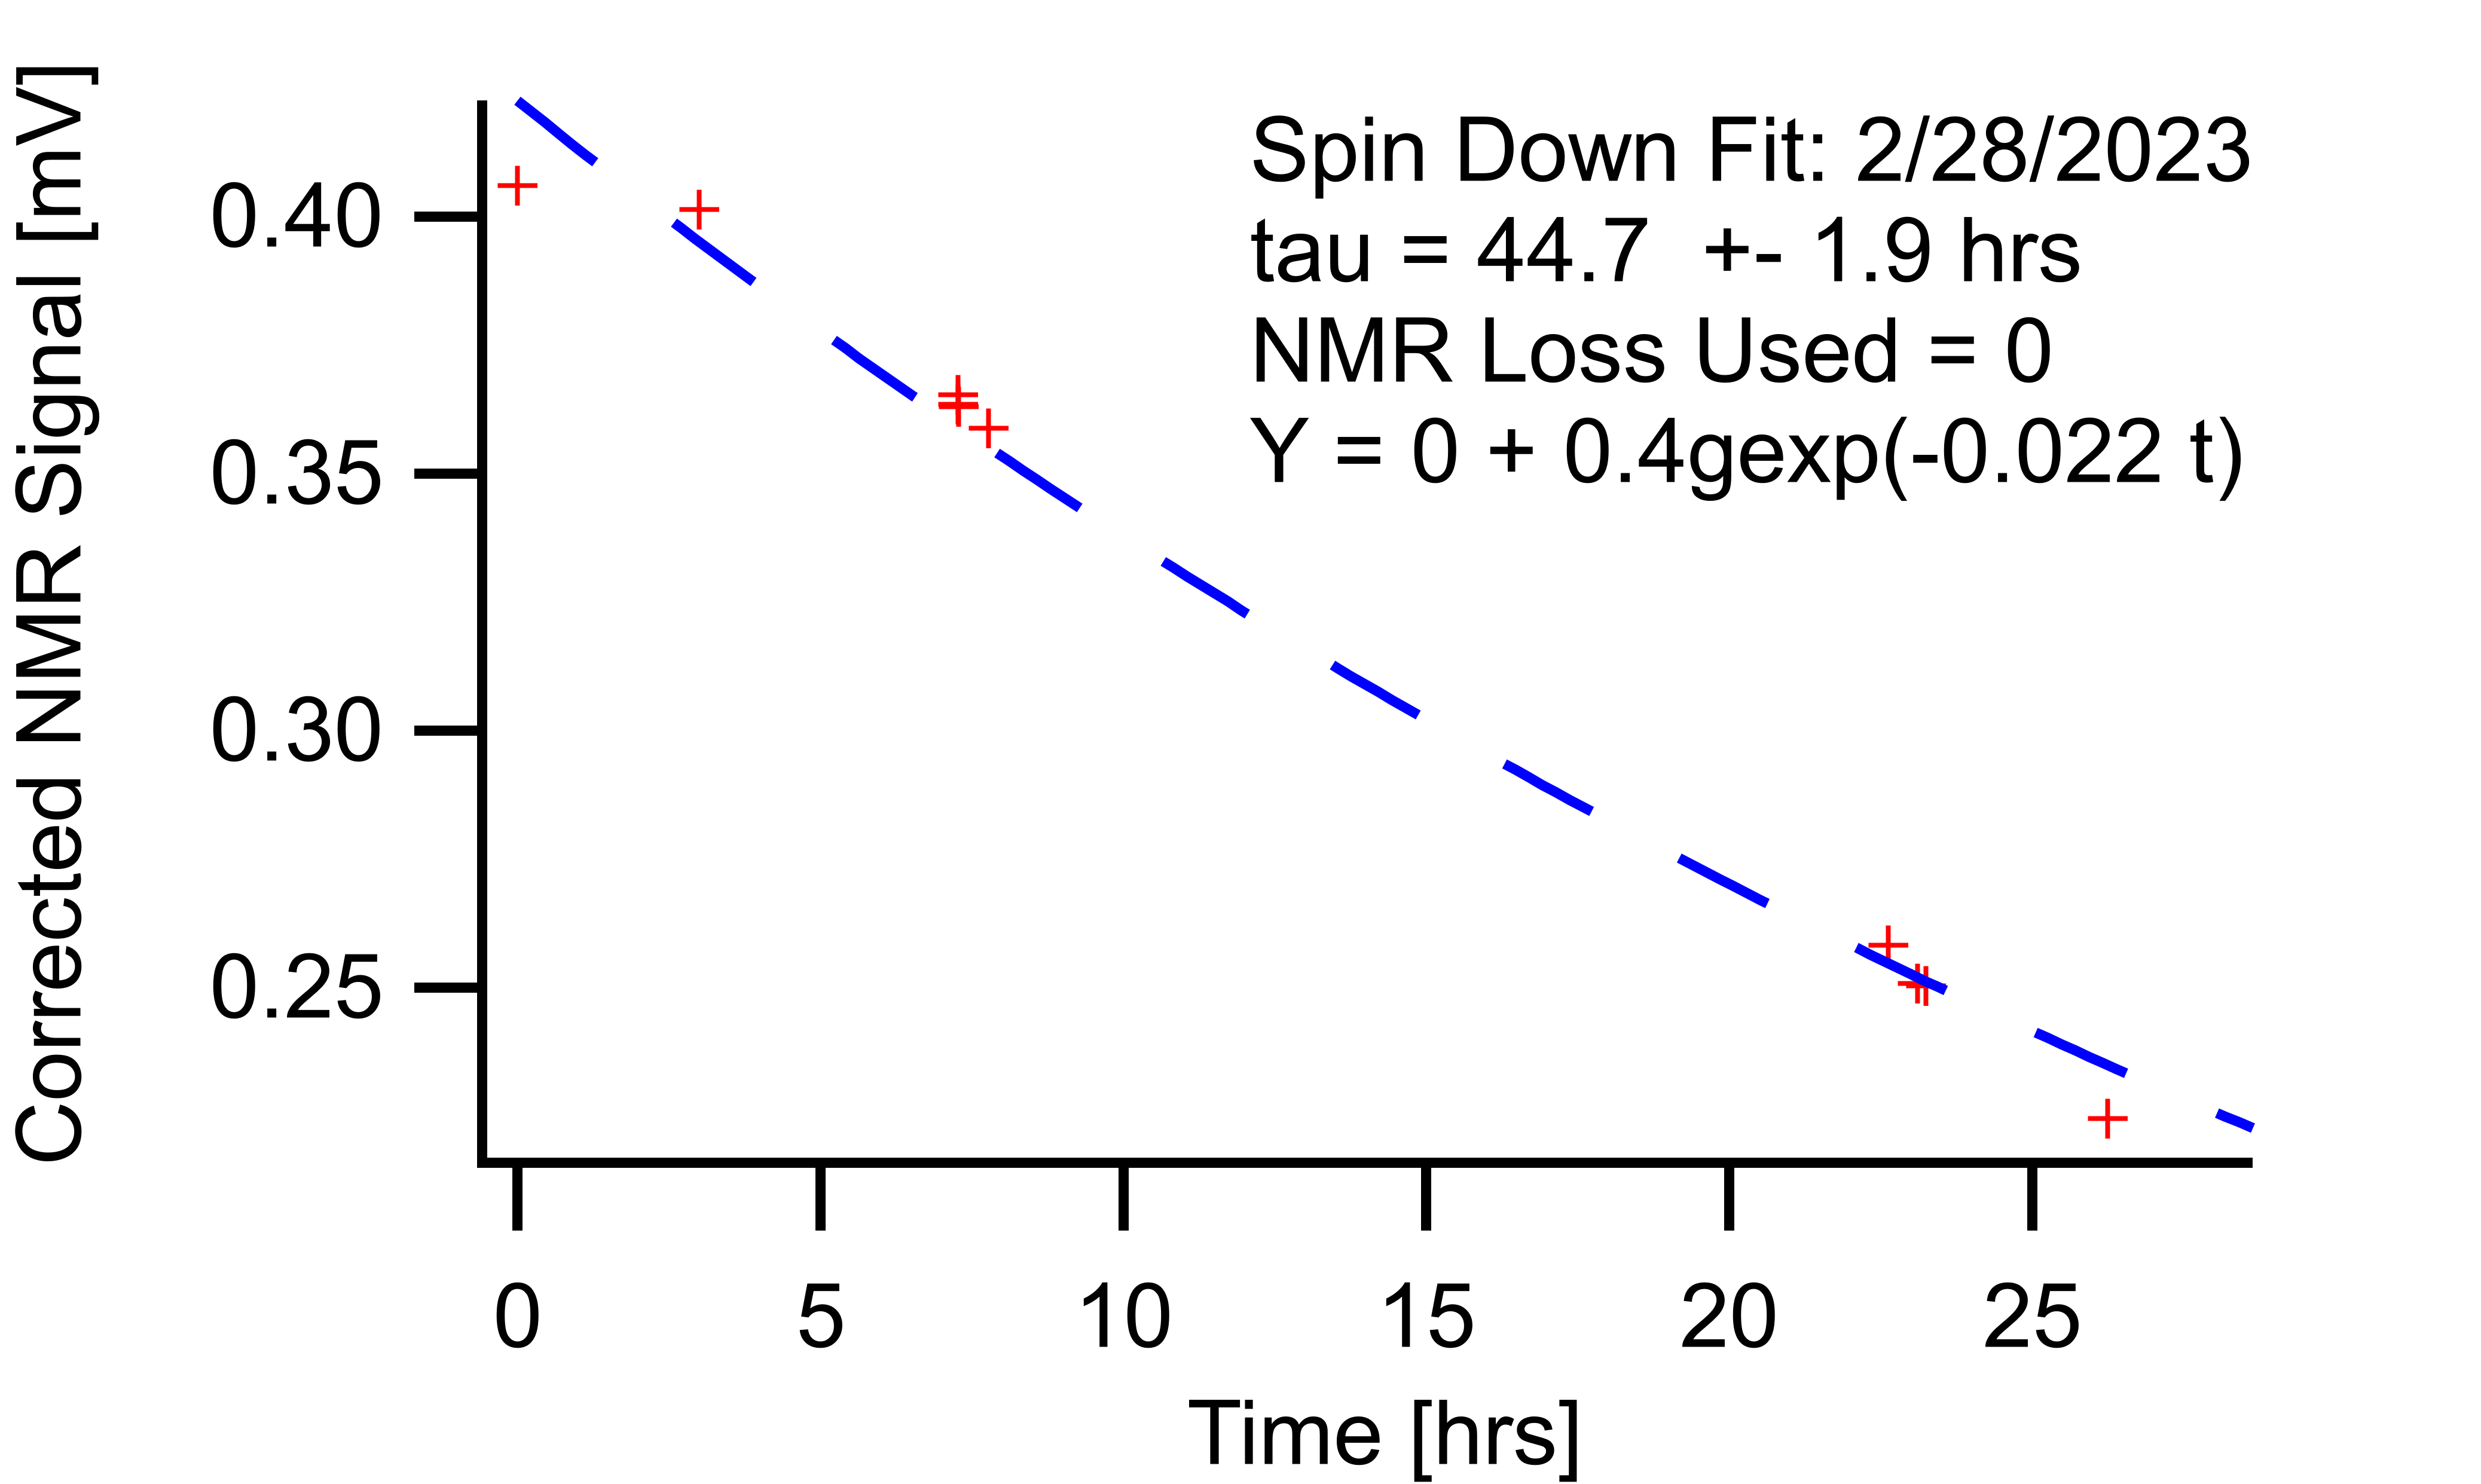
\includegraphics[width=\textwidth]{figures/chapter3-figs/spindown_phase2_2023feb30.png}
    \caption{Response of the FID from the $^3$He over a course of time after the SEOP operation is turned off. The red points are the measured value and the blue curve is the exponential decay fit.}
    \label{fig:spindown}
\end{figure}
\clearpage}

\subsubsection{Adiabatic Fast Passage}

In AFP NMR, an RF magnetic field, applied transverse to the static holding magnetic field of the $^3$He cell, is swept such that it passes through the Larmor frequency of the precessing $^3$He spins in the static magnetic field. Once the RF field sweeps beyond the resonance, the $^3$He polarization is inverted \cite{Abragam1961, Slichter1996}. The RF frequency's frequency sweep and amplitude are optimized to ensure a robust polarization inversion. 

%If a pickup coil transverse to both the static and rf magnetic fields is employed, a signal proportional to the magnetization is obtained. In order to minimize the large background from inadvertent pickup of the applied rf field, the pickup coil must be carefully adjusted to be orthogonal to the driving rf magnetic field. An absolute $^3$He polarization measurement can be obtained if the response of the pickup coil and associated electronics is calibrated using a thermally polarized water cell with exactly the same size and geometry as the $^3$He cell. Despite the extremely small thermal polarization of the order of 10-8 in typical holding fields of a few mT, these calibrations can be performed with uncertainties of a few percent. [In principle the magnitude of the AFP signal could be determined absolutely for a given apparatus, but in a study of this approach discrepancies of between 20\% and 50\% were observed with cell to cell variations (Chen et al., 2011).] Further descriptions of this technique and its application to electron-scattering targets (Chupp et al., 1987; Romalis et al., 1998), polarimetry of low-pressure MEOP cells (Lorenzon et al., 1993), and polarized gas MRI11 have been reported. 

%Whereas losses of a few tenths of a percent are typically encountered for AFP, techniques have been developed to substantially reduce these losses. The primary motivation has been for neutron spin-filter cells that are not actively optically pumped on the beam line, but in which the $^3$He polarization may be frequently inverted during use so as to invert the neutron polarization. Besides the usual optimization of rf magnetic-field strength and sweep rate, the rf field is modulated by a Gaussian envelope during the sweep (Petoukhov et al., 2006; McKetterick et al., 2011). Using this approach,losses of 10-5 per flip have been obtained. In a compact rf solenoid with shielding to confine the rf field, loss as low as 0.03\% was reported (Ye et al., 2013).

The primary usage of the AFP technique has been to invert the polarization of $^3$He cells, to analyze polarized neutron beams or characterize the efficiencies of guide field or spin flipper components in neutron beam experiments. RF frequency techniques have been developed to to perform AFP with high efficiencies. This section describes the AFP setup of the in situ system and the performance results on the polarized $^3$He cell, Soccer. The digitally generated voltage waveform used to provide the frequency sweep as well as a coil pair used to create the RF magnetic field are described. 

A sinusoidal waveform was used to create the required RF magnetic field. The linear frequency spread, $\omega(t)$, was set to sweep through the $^3$He resonance frequency from a range of $\omega_1$ and $\omega_2$, lasting a duration of $t_p$ in secs.
\begin{equation}
    \omega(t) = \frac{\left \lvert \omega_2 - \omega_1  \right \rvert}{2t_p} t + \omega_1 
\end{equation}
In order to ensure an adiabatic transition during the sweep, the amplitude of the sinusoidal wave is modulated with a Gaussian envelope for a rising and falling edge.
\begin{equation}
    B_{RF}(t) \propto \exp\left(   -\frac{[\omega(t) - \omega_L]^2}{\sigma^2}    \right) sin(\omega(t) \cdot t)
    \label{eq:AFPrf}
\end{equation} 
where $\omega_L$ is the $^3$He Larmor frequency and $\sigma$ parametrizes the frequency sweep width of the envelope \cite{Parnell2011}. \Cref{eq:AFPrf} is associated with any generic AFP frequency sweep and was tuned and optimized to work for the AFP requirements of this experiment. 

Previous AFP studies of $^3$He cells in \cite{Petoukhov2006, McKetterick2011} have shown that the maximum amplitude of the envelope should be no more than 10\% of the magnitude of the holding magnetic field, $B_0$. \cite{Petoukhov2006, McKetterick2011} have also shown that for a coil pair that produced a RF field over the required frequency range, $\Delta \omega = \omega_2 - \omega_1$, a Gaussian sweep with a FWHM of 10\% of $\Delta \omega$ created the most efficient spin flips. This amplitude modulated frequency sweep will invert the $^3$He polarization, regardless of the RF field's homogeneity, since it eliminates any high frequency noise in the the AFP pulse \cite{Garwood2001}.

$\Delta \omega$ of the sweep depends on the variation in the the holding magnetic field magnitude. This means that the frequency sweep has to encompass a broad range of the $^3$He resonant frequencies arising from any longitudinal variation in $B_0$ across the $^3$He cell. $\Delta \omega$ can be widened to ensure that the AFP sweep has a small amplitude at the start and at finish of the sweep for the off resonance $^3$He frequencies and at the same time, a large amplitude for the $^3$He resonant frequencies to perform a robust spin flip. Testing in \cite{McKetterick2011} have shown that a frequency range, $\Delta \omega$ of $\frac{\omega_L}{2}$ to $\frac{3\omega_L}{2}$, delivered the most efficient spin flips.

The in situ system has a built in rectangular coil pair used to provide the AFP RF field. The coils made of 18AWG (diameter = 0.0428 inches) copper wire and consist of 15 turns/coil. The total resistance of the coil pair is 0.5$\Omega$ and an inductance of 0.317 mH. The Q-factor as $\frac{\omega_L L}{R}$, where $L$ is the inductance and $R$ is the resistance, comes out to be 68, indicating the the RF coil pair is operating in the inductive regime with minimal power loss to impedance. This setup is shown in \cref{fig:NMRsetup}. The $^3$He has a reuced gyromagnetic ratio of 3.24 kHz/G, therefore, the resonant frequency for the 12.7 G holding magnetic field created by the Merritt coil is 41.16 kHz. These frequencies were created  with the same digital I/O card as used in the FID NMR. Using the IgorPRO programming package, a digital waveform generator, was used to to generate the AFP sweep waveform based on the parameters of desired AFP sweep. A frequency binning of 1 microhertz was used to avoid aliasing. This fine binning was possible because of the sampling rate of the digital I/O card used. The I/O card converts the digital AFP waveform to an analog waveform, which is sent to the AFP coil pair via a power amplifier set to a 50$\times$ gain. This setup is illustrated in \cref{fig:NMRsetup}. The parameters shown in \cref{tab:AFP_params} were used to generate an AFP pulse, shown in \cref{fig:AFPtime}, from the DAQ board as:
\begin{equation}
 \begin{aligned}
    F_{AFP}(t_i)  = V_{RF} & \times \exp\left( -\frac{ \left[\left(f_{min}-R_{sweep} \times t_i \right)- f_{cent} \right]^2 }{f_{FWHM}^2}    \right) \\
    & \times sin \left(2 \pi \left(f_{min} + \frac{1}{2} R_{sweep} \times t_i \right) \times t_i \right)
\end{aligned}   
\end{equation}
where
\begin{equation}
    t_i = \cfrac{f_{max}-f_{min}}{\cfrac{R_{sweep}}{t_{step}}}
\end{equation}
and the total time of the AFP pulse duration comes out to be:
\begin{equation}
    t_{total} = \frac{f_{max}-f_{min}}{R_{sweep}}
\end{equation}

\afterpage{
\begin{table}
\centering
\caption{List of parameters used for AFP NMR to invert the polarized $^3$He.}
\label{tab:AFP_params}
\begin{tabular}{@{}lc@{}}
\toprule
AFP Parameters               & AFP Parameter Values \\ \midrule
Center Frequency {[}Hz{]}    & 41160                \\
Frequency Sweep Rate {[}kHz/sec{]}           & 50-200               \\ 
Freq. FWHM {[}Hz{]}          & 7000               \\
Minimum Frequency {[}Hz{]}           & 0.6 $\times$ 41160                     \\
Maximum Frequency {[}Hz{]}          & 1.5 $\times$ 41160                  \\
Amplitude {[}V{]}            & 2.0               \\
A0 timestep {[}sec{]}           & $1\times10^{-6}$       \\ 
\bottomrule
\end{tabular}
\end{table}
\clearpage}

\afterpage{
\begin{figure}
    \centering
    \includegraphics[width=\textwidth]{figures/chapter3-figs/AFP_waveintime.png}
    \caption{Modulated RF pulse used for AFP based on the parameters in \cref{tab:AFP_params}.}
    \label{fig:AFPtime}
\end{figure}
\clearpage}

There are two indicators that determine the performance of an AFP flip. The first is to determine whether the AFP has reversed the polarization of the $^3$He nuclei and the second is to measure the relative loss in $^3$He polarization after an AFP spin flip sequence \cite{McKetterick2011, Parnell2008}. The FID NMR described in the previous section was used to characterize the performance of the AFP flip sequence. The change of phase of the FID signal determines the relative polarization state of the $^3$He analyzer cell. The polarized $^3$He FID signal and spin inverted $^3$He FID signal should show a difference in phase angle of $180 \degree $ indicating that a change in $^3$He polarization has taken place \cite{Parnell2008, Parnell2011}. The FID response measured from Soccer, before and after AFP pulse was deployed, is shown \cref{fig:AFPflip}. The before and after FID responses show a $180 \degree $ change in phase, indicating a successful inversion of $^3$He polarization from an AFP pulse.

%The initial amplitude of the FID is found by fitting the data to the equation :
%%    f(t) = \frac{1}{2} V_{pp} sin(\omega_L t + \phi) \exp\left( \frac{-t}{T_2^*}    \right)
%    \label{eq:FID}
%\end{equation}
%where $V_{pp}$ is the peak to peak voltage caused by the spin precession tipping from the FID pulse and $\omega_L$ is the Larmor frequency and $\phi$ is the phase of the sinusoidal wave. The exponential decay envelope of the FID response has a transverse relaxation time constant, $T_2^*$, which is dependent upon the inhomogeneities in the holding field, $B_0$. The decay in FID amplitude was plotted against time and fitted to the \cref{eq:FID}, to extract the max amplitude, frequency, phase and $T_2^*$. 

%\Cref{fig:AFPflip} shows that although the two $^3$He polarization states should be experiencing the same magnetic field and the same gradients, the observed FID signals for the unflipped and flipped states have slightly different $T_2^*$ time. This can be attributed to radiation damping effects \cite{Augustine2002} and the onset of masing in the high energy state \cite{Chupp1994}. There may also be contributions to the local magnetic field due to the reversal of the bulk $^3$He polarization. 

The relative loss in $^3$He polarization arising from performing AFP NMR was measured by recording FID signals before and after performing 10 consecutive AFP sweeps. The initial tests showed losses of 0.053\% loss in $^3$He polarization per flip. This loss is minimal and adequate for the in situ system.

When AFP is performed, the $^3$He polarization becomes flipped with respect to the holding magnetic field. This means that the D1 transition is now from $m_s=-1/2$ and the circularly polarized light, $\sigma_+$ is no longer useful. As a matter of fact it will depolarize the alkali and hence, the $^3$He. Therefore, the LCR was adjusted to provide $\sigma_-$ D1 circular polarized light every time $^3$He polarization was flipped with respect to $^3$He and vice versa.

\afterpage{
\begin{figure}
     \centering

     \begin{subfigure}{0.9\textwidth}
         \centering
         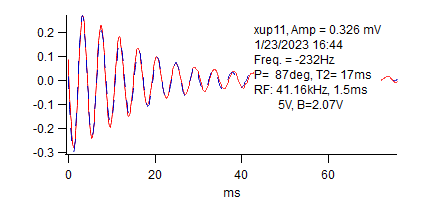
\includegraphics[width=0.9\textwidth]{figures/chapter3-figs/xup_graph.png}
         \caption{FID response prior to an AFP pulse.}
         \label{fig:FIDpriorAFP}
     \end{subfigure}
     \hfill
     \begin{subfigure}{0.9\textwidth}
         \centering
         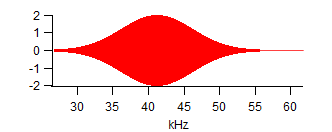
\includegraphics[width=0.75\textwidth]{figures/chapter3-figs//AFPF_RF.png}
         \caption{AFP Pulse used to invert $^3$He polarization.}
         \label{fig:AFPpulsefreq}
     \end{subfigure}
     \hfill
     \begin{subfigure}{0.9\textwidth}
         \centering
         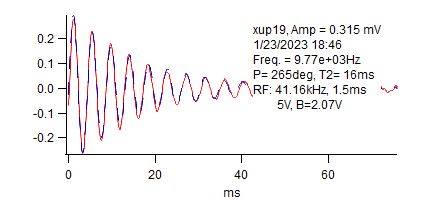
\includegraphics[width=0.9\textwidth]{figures/chapter3-figs/xup_graph_postafp.png}
         \caption{FID response post an AFP pulse.}
         \label{fig:FIDpostAFP}
     \end{subfigure}
        
        \caption{Inversion of $^3$He polarization in Soccer. Notice the 180$\degree$ phase change from (a) to (c) after the AFP pulse (b) is applied. Red curve is the measured response and the blue curve is the fit.}
        \label{fig:AFPflip}

\end{figure}
\clearpage}

\subsection{Electron Paramagnetic Resonance Spectroscopy}

Electron Paramagnetic Resonance Spectroscopy is used as an additional diagnostic to characterize the $^3$He polarization. EPR spectra is obtained by detecting the fluorescence from a polarized $^3$He cell under the application of transverse RF magnetic field, which slightly changes the alkali polarization by sweeping through the alkali Zeeman resonances \cite{Romalis1998, Chann2002a, Kramer2007}. The polarized alkali serve as insitu comagnetometers of the classical dipole magnetization produced by the polarized $^3$He. The field experienced by the polarized alkali from the polarized $^3$He is \cite{Romalis1998, Schaefer1989, Barton1994}:
\begin{equation}
    B_{He} = \mu_{He} \kappa_{eff} [He] P_{He}
\end{equation}
where $\mu_{He}$is the $^3$He magnetic moment, and $\kappa_{eff}$ is defined as:
\begin{equation}
    \kappa_{eff} = \kappa_0 + \frac{3}{8\pi}C-1
\end{equation}
where $\kappa_0$ is a dimensionless proportionality factor \cite{Romalis1998} and $C$ is the constant for a cylindrical $^3$He cell \cite{Chann2002} with radius, $r$, and length, $l$, like Soccer as:
\begin{equation}
    C = \frac{8\pi}{3} \left( \frac{3}{2} \left( \sqrt{1 + \frac{r}{l}^2} - \frac{r}{l} \right)  \right)  
\end{equation}

The field $B_{He}$ produces an EPR frequency shift \cite{Romalis1998}:
\begin{equation}
\label{eq:EPRshift}
    \Delta \nu_{EPR} = \gamma_A B_{He} = \frac{\gamma_e}{2 I_A + 1} B_{He}
\end{equation}
where $\gamma_e =$28 GHz/T is the electron's gyromagnetic ratio. This means that $^3$He can be extracted via the EPR frequency shift. $\kappa_0$ has been measured for alkali atoms and is shown in \cref{tab:spinexrate} \cite{Gentile2017}. 

Since the alkali are also highly polarized and undergoing spin exchange with $^3$He, the EPR spectrum becomes proportional to the square of the RF magnetic field \cite{Romalis1998}. For small holding magnetic fields, this leads to a splitting between EPR levels arising from the second-order Zeeman effect in B \cite{Gentile2017} as: 
\begin{align}
    x \frac{\gamma_e^2}{\Delta E_{hf}} B^2
\end{align}
where $\Delta E_{hf}$ is the hyperfine splitting and 
\begin{align}
x = \frac{4(2m-1)}{(2I_A+1)^2} =
    \begin{cases}
        \frac{2}{9} & \text{for $^{85}$Rb with I$_A$ = 5/2}\\
        \frac{1}{2} & \text{for $^{87}$Rb and K with I$_A$ = 3/2} 
    \end{cases}
\end{align}

In SEOP, the the hyperfine levels at play during EPR are m=$F_{max}$ $\rightarrow$ $F_{max}-1$ and $F_{max}-1$ $\rightarrow$ $F_{max}-2$, where $F_{max} = I_A+1/2$ is the maximum angular momentum state of the alkali under D1 transition of alkali \cite{Romalis1998, Gentile2017}. The F$_{max}$ line is unperturbed, while the $F_{max}-1$ line is broadened from the spin exchange \cite{Appelt1999}. As mentioned earlier, even though the alkali excited to the P state are mostly quenched by N$_2$, a small fraction of them still decay by fluorescence. Thus, if the RF magnetic field tuned at the alkali resonance frequency induces a transition from F$_{max}$, m=$F_{max}$ to F$_{max}$, m = $F_{max}-1$, then the number of the alkali atoms in m = $F_{max}-1$, which can absorb light will be increased and hence, the fluorescence will increase \cite{Romalis1998, Gentile2017}. In practice, the D1 light of the laser dominates the D1 fluorescence emission of the $^3$He cell. Therefore, alkali's D2 transition emission is used to measure the EPR frequency shift as a function of RF frequency sweep. Since the EPR shift depends on the $^3$He magnetization, AFP flip on $^3$He polarization with respect to the magnetic field is performed to isolate the EPR frequency shift from other effects \cite{Romalis1998}. This gives double the EPR frequency shift due to the AFP flip.

%There are two ways to measure the EPR frequency shift: the Amplitude Modulation (AM) measurement and the Frequency Modulation (FM) measurement. The AM method measures the intensity of the D2 emission with respect to the RF frequency while the FM method measures the derivative of the intensity with respect to the frequency.

The setup used for the EPR for the in situ $^3$He system is shown in \cref{fig:NMRsetup}. A function generator programmed digitally was used to create the modulated RF field. The RF field was applied to the $^3$He cell by a circular coil, about the size of the $^3$He cell, mounted on one side of the $^3$He cell. The fluorescence from the $^3$He cell was measured using a photodiode with a D2 filter placed along the exposed face of the $^3$He cell. The signal from the photodiode was sent to the lock-in amplifier, as mentioned in the previous section, and referenced to the modulation frequency of the function generator. By scanning the RF frequency, the change in the measured photodiode intensity as a function of frequency was recorded. When the RF frequency sweeps through the EPR resonance frequency, the measured signal should reach the maximum and therefore, the EPR frequency can be extracted.

Unfortunately, after performing many sweeps and trying several parameters, a photodiode signal was not observed. Possible causes for this could be the presence of gradeints in the holding magnetic field, which can change the $^3$He magnetization, change in cell temperature as the $\kappa_0$ has slight temperature dependence and can change $ \Delta \nu_{EPR}$ by 0.14\%/$\degree$C, or the the $^3$He density of the cell Soccer is too low to extract an EPR response. Further diagnosis of this problem need to be performed.


\subsection{Neutron Transmission}

There is a large neutron absorption cross section for $^3$He, which arises from a broad($\Gamma$=400 keV) , unbound, resonance ($J^{\pi}=0^{+}$) located 650 keV below the neutron binding energy of the $^4$He$^{*}$ intermediate state, that yields a proton and a triton \cite{Csoto1997}. The reaction can be shown as:
\begin{equation}
    n+ {^3He} \rightarrow {^4He^*} \rightarrow t + p
\end{equation}
Furthermore, the ground state of $^3$He wavefunction is dominated by the singlet state, in which the spins of the two protons negate due to the exclusion principle, and the $^3$He nuclear spin is effectively given by the unpaired neutron \cite{Bissey2002, Friar1990}. This leads to a strong spin dependence in the absorption cross section; 5333 barns for 25 meV neutron capture on $^3$He with antiparallel spins and nearly zero for parallel spins \cite{Passell1966}. The ratio of absorption cross section to the total reaction cross sections for this reaction has been found to be near unity with an error of less than a percent, indicating that absorption mechanism dominates the reaction \cite{Huber2014} and non-resonant scattering cross section is small, measured to be 6 barns \cite{Mughabghab1981} \footnote{The neutron and $^{3}He$ capture can also undergo another reaction branch, $n+ {^3He} \rightarrow {^4He} + \gamma$, but the cross section for this branch is in microbarns \cite{Zurmuhle1963}.}. 

Hence for an ideal 100\% polarized $^3$He cell, neutrons with spins antiparallel to $^3$He polarization will get captured, while neutrons with spins parallel to $^3$He polarization will transmit through the NSF. The resulting transmitted neutrons from the NSF will be 50\% of the initial intensity and 100\% polarized, with respect to the guide magnetic field. Subsequently, imperfect $^3$He polarization will be inefficient in discriminating the neutron polarization as well as decrease the neutron transmission. The efficacy of the NSF can be changed by picking the cell thickness, i.e. the neutron opacity, based on the needs of the experiment. In addition to being spin dependent, the n-$^3$He absorption cross section, is inversely proportional to the neutron wavelength as $\sigma_0/\lambda_0$ in units of 10$^{-24}$ cm$^2$, hence longer wavelength (lower kinetic energy) neutrons require lesser opacities. For NSFs, opacity is adjusted by varying the pressure, $P$, in bars of $^3$He (i.e. the $^3$He number density, $n_{He}$, in units of cm$^{-3}$) and the length, $l$, in cm of the cell for a given neutron wavelength, $\lambda$, in \AA. The opacity, $\zeta$, can be written as:
\begin{equation}
    \zeta = -n_{He}l\frac{\sigma_0}{\lambda_0}\lambda(t) = 0.073 ~\text{bar$^{-1}$  cm$^{-1}$  \AA$^{-1}$} \cdot P \cdot l \cdot \lambda
    \label{eq:opacity}
\end{equation}
Hence, the transmission of an unpolarized monochromatic neutron beam through an unpolarized $^3$He cell can be determined from:
\begin{equation}
    T_{unpol} = T_e e^{-\zeta}
    \label{eq:Tunpol}
\end{equation}
where $T_e$ is the transmission through an empty glass cell, which for GE180 glass has been measured to be 88\% $\pm$ 2\% \cite{Chupp2007}.

The $^3$He polarization can be defined \footnote{Assuming no coherence between the two spin states.} as:
\begin{equation}
P_{He} = \frac{n_{He}^{\uparrow} - n_{He}^{\downarrow}}{n_{He}^{\uparrow} + n_{He}^{\downarrow}} =   \frac{n_{He}^{\uparrow} - n_{He}^{\downarrow}}{n_{He}}
\end{equation}
where $n_{He}^{\uparrow}$ is the number density of spin up particles and $n_{He}^{\downarrow}$ is the number density of spin down particles. The polarized $^3$He densities can be expressed in terms of $^3$He polarization as $n_{He}^{\uparrow} = \frac{n_{He}}{2}(1+P_{He})$ and  $n_{He}^{\downarrow}  = \frac{n_{He}}{2}(1-P_{He})$. If we now assume that $^3$He cell is polarized, then for an incident unpolarized neutrons, $N_0 = N_\uparrow + N_\downarrow$, the neutron intensity from the transmission for the two neutron spin states through the polarized $^3$He cell is given by:
\begin{equation}
    N_\uparrow = \frac{N_0 T_e}{2} e^{-\zeta} e^{\zeta P_{He}}
\end{equation}
and
\begin{equation}
   N_\downarrow = \frac{N_0 T_e}{2} e^{-\zeta} e^{-\zeta P_{He}}
\end{equation}
Now, with the neutron polarization defined \footnote{Again, assuming no coherence between the two spin states.} as:
\begin{equation}
    P_n = \frac{N_\uparrow - N_\downarrow}{N_\uparrow + N_\downarrow}
\end{equation}
the analyzing/polarizing, $P_n^{He}$, power of the $^3$He cell becomes
\begin{equation}
    P_n^{He} = \tanh{\left(\zeta P_{He}\right)}
    \label{eq:anal_power}
\end{equation}
and the transmission of the unpolarized beam through a polarized $^3$He cell becomes:
\begin{equation}
       T_{pol} = T_{unpol} \cosh{\left(\zeta P_{He}\right)}
       \label{eq:Tpol}
\end{equation}
Using the hyperbolic trigonometric identity, $1+\tanh^2{x} = \sech^2{x}$, $P_n^{He}$ can be expressed as:
\begin{equation}
    P_n^{He} = \sqrt{1 - \left(\frac{T_{unpol}}{T_{pol}} \right)^2}
    \label{eq:anal_power2}
\end{equation}
This implies that, $P_n^{^3He}$, can be accurately determined with only a relative neutron transmission measurements through a polarized $^3$He cell \cite{Greene1995, Coulter1990, Jones2000}. Because of the wavelength dependence, neutron transmission measurements can be performed with either monochromatic beams or with the time-of-flight (TOF) analysis for pulsed neutron beams.

For an incident neutron beam of 8.9~\AA\ and the Soccer cell parameters, the expected transmission and analyzing power analyzing of the cell soccer as a function of $^3$He polarization can be determined. This is shown in \cref{fig:soccer_exp}. The figure illustrates two important features of polarized $^3$He based neutron polarimetry. First, the higher the $^3$He polarization, the higher transmission of unpolarized neutrons from a polarized $^3$He cell is expected. Secondly, the higher the $^3$He polarization, the higher the analyzing power of the $^3$He cell (i.e. the $^3$He cell can discriminate between two neutron spin states more efficiently and provide a better spin contrast.)

\afterpage{ 
\begin{figure}
    \centering
    \includegraphics[width=\textwidth]{figures/chapter3-figs/SoccerLonestarcomparson.png}
    \caption{The analyzing power, $P_n^{^3He}$, and transmission, $\frac{T_{pol}}{T_{unpol}}$, as a function of $^3$He polarization for the cell Soccer with 0.8 bar pressure, 6.62 cm in length and an 8.9~\AA\ incident neutron beam.}
    \label{fig:soccer_exp}
\end{figure}
\clearpage}

\afterpage{
\begin{figure}
    \centering
    \begin{subfigure}[b]{0.75\linewidth}
        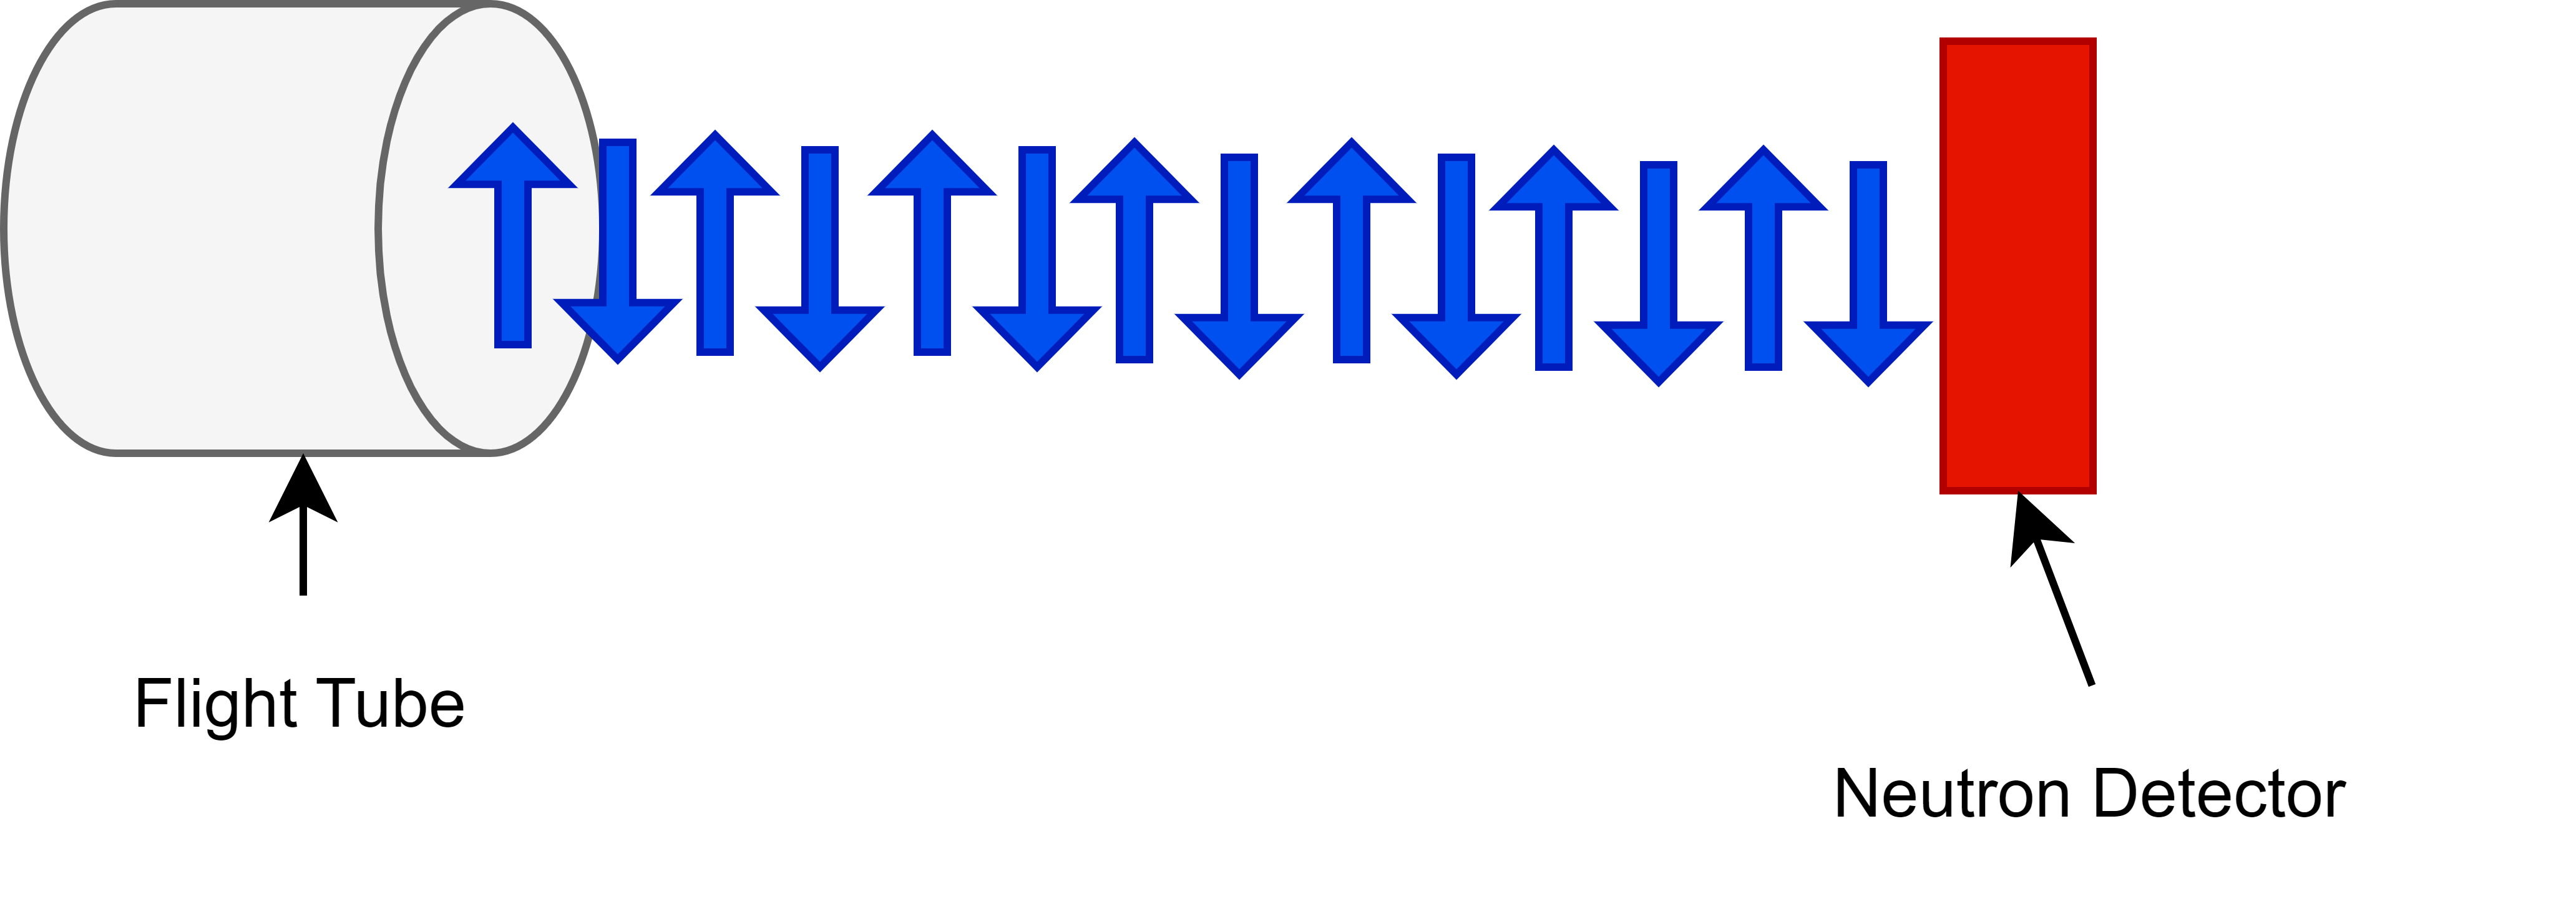
\includegraphics[width=\linewidth, height=4.5cm]{figures/chapter3-figs/unpolbeam_nocell.png}
    \caption{$N_0$}
    \label{fig:directbeam}
    \end{subfigure}
    \hfil
    \begin{subfigure}[b]{0.75\linewidth}
        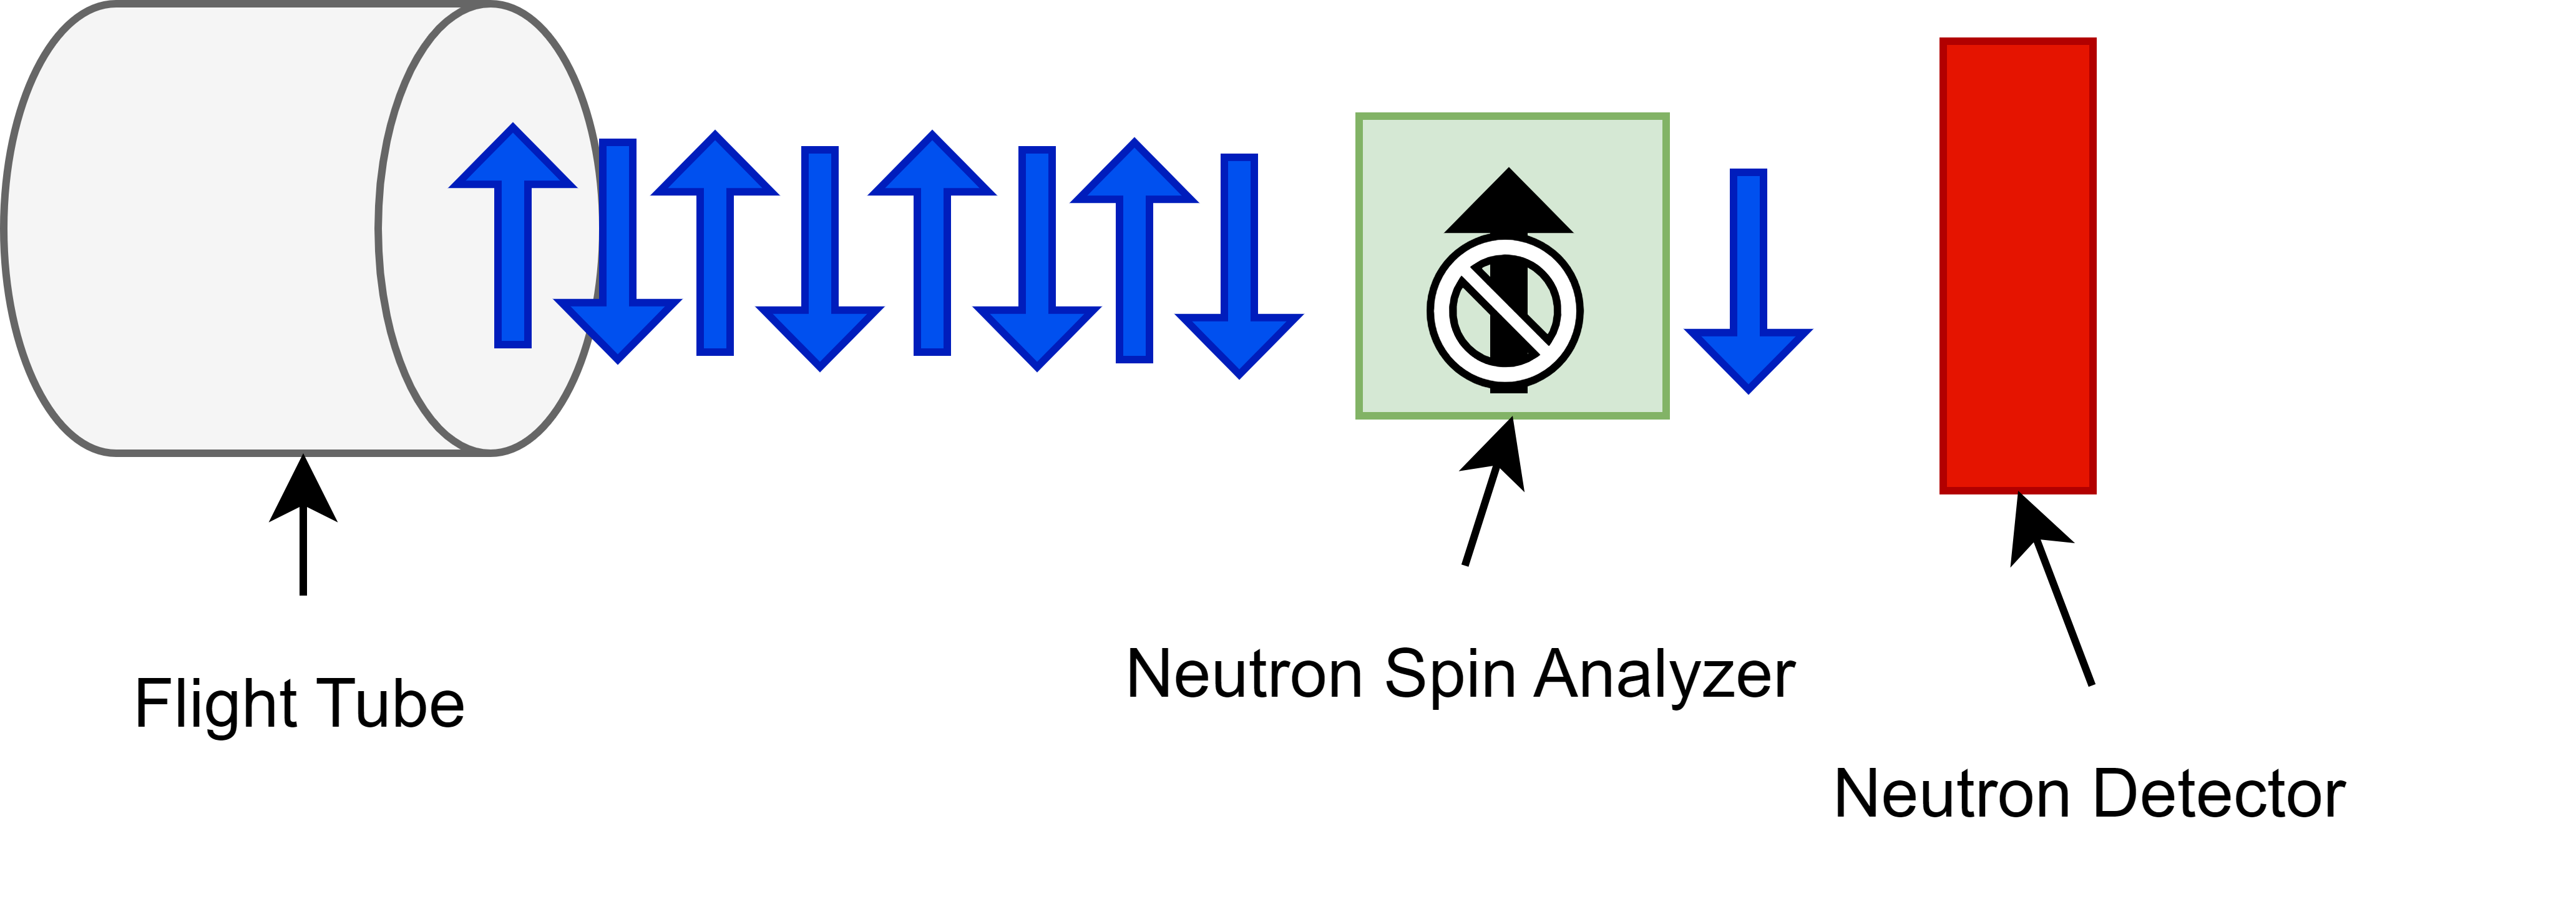
\includegraphics[width=\linewidth, height=4.5cm]{figures/chapter3-figs/unpolbeam_unpolcell.png}
    \caption{$T_{unpol}$}
    \label{fig:unpolcell}
    \end{subfigure}
    \begin{subfigure}[b]{0.75\linewidth}
        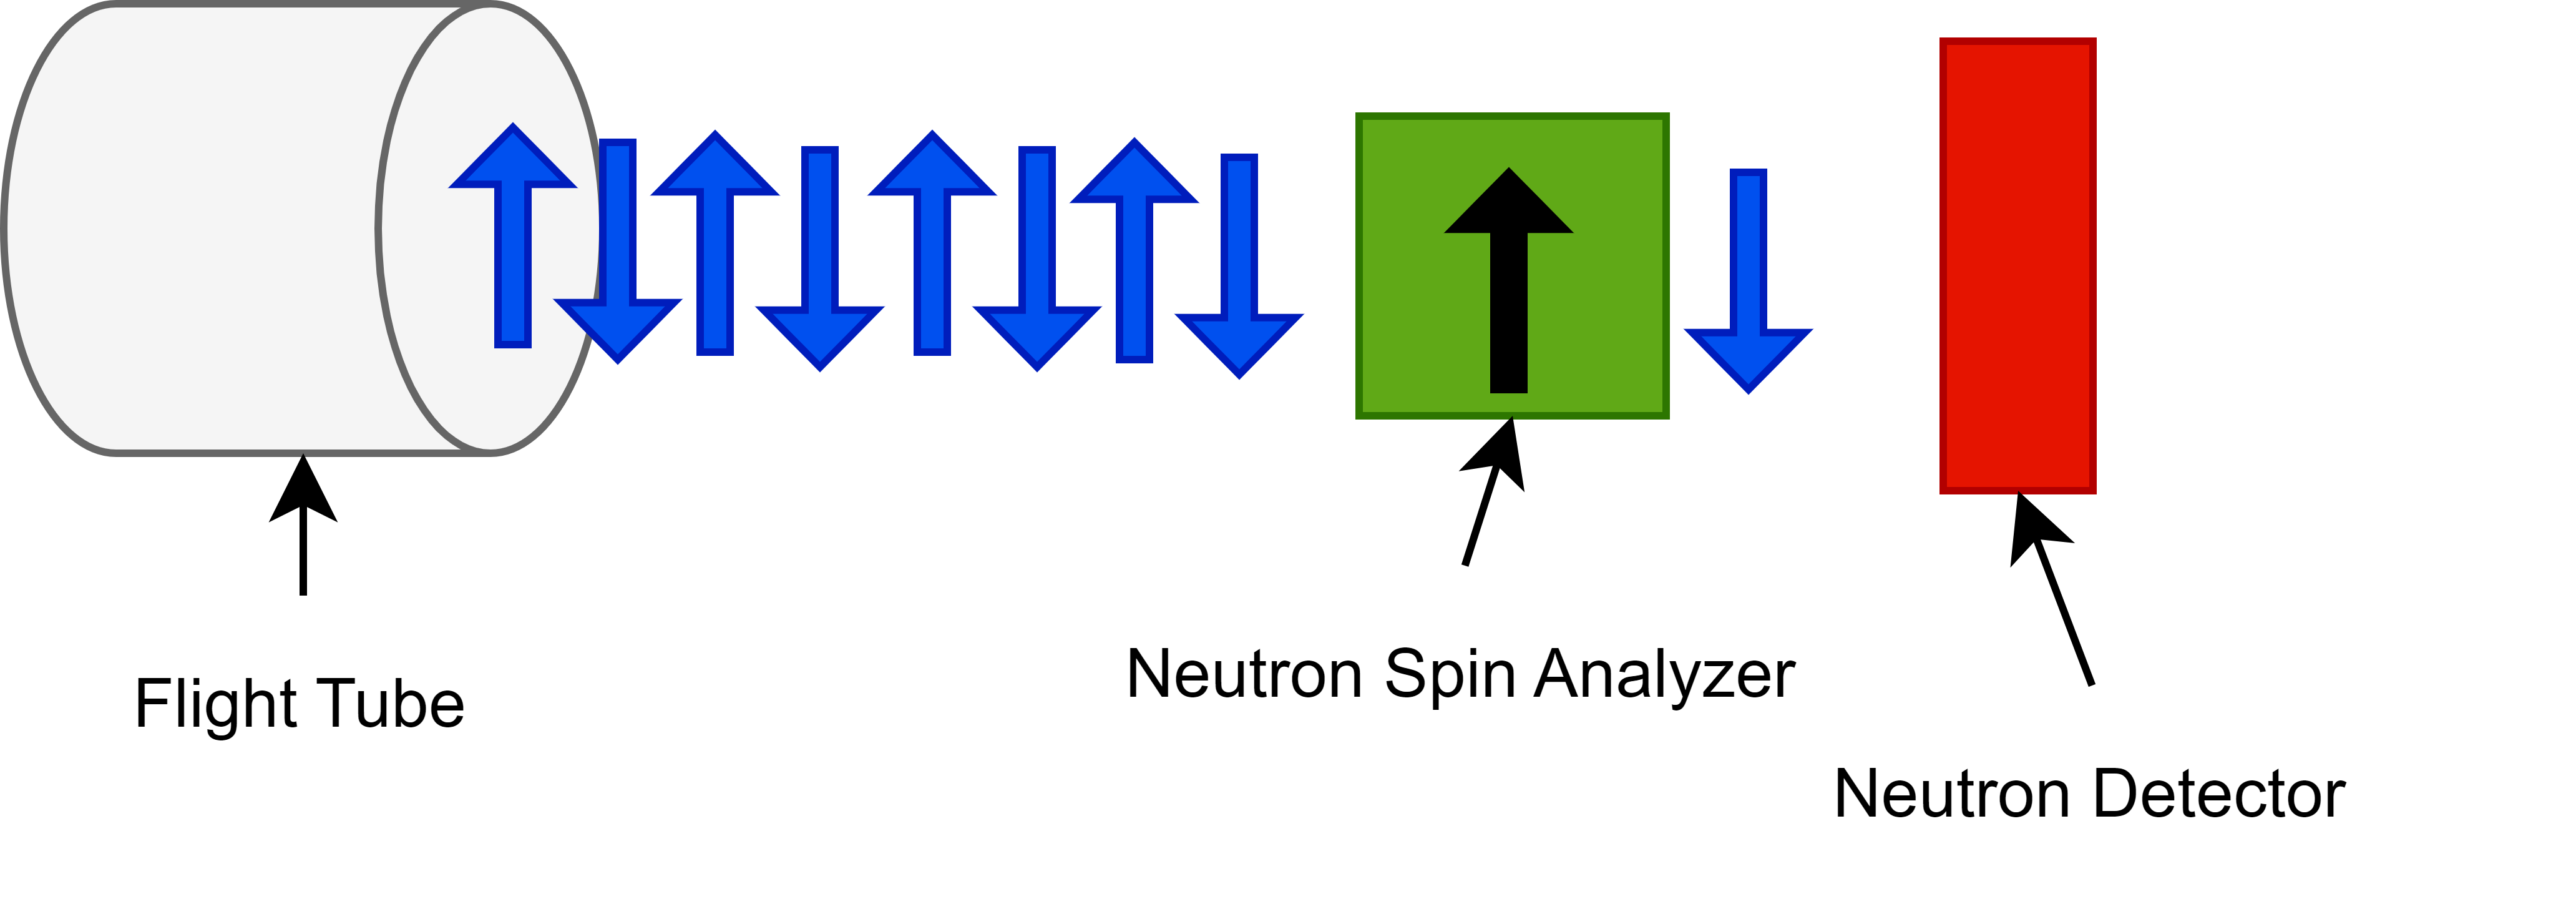
\includegraphics[width=\linewidth, height=4.5cm]{figures/chapter3-figs/unpolbeam_polcell.png}
    \caption{$T_{pol}$}
    \label{fig:polbeam}
    \end{subfigure}
\caption{Transmission of unpolarized neutrons through $^3$He cell for the absolute determination of $^3$He polarization.}
\label{fig:unpol_scheme}
\end{figure}
\clearpage}


\afterpage{
\begin{table}
\centering
\caption{Summary of the transmission measurements of 8.9~\AA\ unpolarized neutron beam through the different configurations of polarized $^3$He cell for the setup shown in \cref{fig:unpol_scheme}.}
\label{tab:unpolbeam}
\begin{tabular}{@{}lccc@{}}
\toprule
State & Beam Polarization State & Analyzer Polarization State & Neutron/s/MW \\ \midrule
$N_0$ & Unpolarized & Not Present & 4489 \\
$T_{unpol}$ & Unpolarized & Unpolarized & 189 \\
$T_{pol}$ & Unpolarized & Polarized & 263 \\ \bottomrule
\end{tabular}
\end{table}
\clearpage}

As part of the in situ system, $^3$He cell Soccer was placed in the unpolarized 8.9~\AA\ monochromatic neutron beamline to characterize the $^3$He polarization as well as the analyzing power. The setup for the transmission of unpolarized 8.9~\AA\ neutrons through the various configuration of $^3$He cell from \cref{eq:Tpol} and \cref{eq:anal_power} is illustrated in \cref{fig:unpol_scheme}. The measurement results are given in \cref{tab:unpolbeam}. Based on these results, the fractional transmission of the unpolarized 8.9~\AA\ neutron beam through an unpolarized Soccer cell, as stated in \cref{eq:Tunpol}, was measured to be:
\begin{equation}
    T_{unpol} = 0.042
\end{equation}
From \cref{eq:Tpol}, the ratio of the transmission of unpolarized neutrons through an polarized Soccer cell to the transmission of unpolarized neutrons through a unpolarized Soccer cell was found to be:
\begin{equation}
    \frac{T_{pol}}{T_{unpol}} = 1.39
\end{equation}
From this, \cref{eq:Tpol} was used to determine the fractional absolute $^3$He polarization as:
\begin{equation}
    P_{He} = 0.27
\end{equation}
and subsequently, \cref{eq:anal_power} was used to extract the fractional analyzing power of Soccer cell as:
\begin{equation}
    P_n^{^3He} = 0.70
\end{equation}
Once absolute $^3$He polarization of the Soccer cell is determined from neutron transmission, it can be used as a reference to calibrate NMR-based relative $^3$He polarization measurements of $^3$He cells with typical accuracy of a few percent \cite{Chen2011}. This method is used extensively in the next chapter, therefore, a more detailed overview and results will be presented there.

%The transmission of unpolarized neutron beam can be approximated from the transmission of a polarized neutron beam as:
%\begin{equation}
 %   \frac{T_{unpol}}{T_{pol}} = \frac{T_0}{ \cfrac{ T_\uparrow + T_\downarrow}{2}}
%\end{equation}
%where $T_0$ is the transmission of polarized neutrons through unpolarized 3He cell, $T_\uparrow$ is the transmission of polarized neutrons through polarized 3He cell and $T_\downarrow$ is the transmission of spin flipped neutrons through a polarized 3He cell. The analyzing power of the 3He from a polarized neutron beam:
%\begin{equation}
%    P_n^{He} = \sqrt{1 - \left(\frac{2T_0}{T_\uparrow + T_\downarrow} \right)^2} = \frac{\sqrt{\left(R_\uparrow + R_\downarrow \right)^2-4}}{R_\uparrow + R_\downarrow}
%\end{equation}
%where $R_\uparrow = \frac{T_\uparrow}{T_0} $  and  $ R_\downarrow = \frac{T_\downarrow}{T_0} $.

%However, the total analyzing power of the polarizer and analyzer is:
%\begin{equation}
%    \epsilon_{ST} \cdot \epsilon_{SF} \cdot P_{n} \cdot P^{He}_{n} = \frac{R_{\uparrow}-R_{\downarrow}}{R_{\uparrow}+R_{\downarrow}}
%\end{equation}
%Cannot separate spin transport efficiency with beam polarization.
%\begin{equation}
%    \epsilon_{ST} \cdot P_{n} \rightarrow P_{n} = \frac {1}{ \epsilon_{SF} \cdot P^{He}_{n} } \left( \frac{R_{\uparrow} - R_{\downarrow}}{R_{\uparrow}+R_{\downarrow}}  \right) =  \frac{R_{\uparrow} - R_{\downarrow}}{ \sqrt{ \epsilon_{SF}^2\left(R_\uparrow + R_\downarrow \right)^2 - 4\epsilon_{SF}^2 }  } 
%\end{equation}
%where $ \epsilon_{SF} = \frac{1}{2} \left(  1 - \frac{R_\downarrow}{R_\uparrow}     \right) $, is the efficiency of the spin flipper used to flip $R_\uparrow$ to $R_\downarrow$.











































    %!TEX root = ../thesis.tex
%*******************************************************************************
%****************************** Third Chapter **********************************
%*******************************************************************************
\chapter{Neutron Polarization \& Transmission Measurement}
\label{ch:PT}

% **************************** Define Graphics Path **************************
\ifpdf
    \graphicspath{{figures/chapter4-figs/Raster/}{figures/chapter4-figs/PDF/}{figures/chapter4-figs/}}
\else
    \graphicspath{{figures/chapter4-figs/Vector/}{figures/chapter4-figs/}}
\fi

The nEDM@SNS experiment will employ the Magnetic Field Module (MFM), as described in \cref{ch:nEDM}, to provide the required magnetic field environment for the nEDM@SNS experiement\cite{Ahmed2019}. As shown in \cref{fig:MFM}, the nEDM MFM along with the accompanying cryostat (both of which from henceforth will be referred to as the combined cryomagnet) is made of several concentric nested vessels \cite{Ahmed2019}. As shown in \cref{fig:PT_pic}, the monochromatic polarized neutron beam will traverse the nEDM cryomagnet system from the thin metal beam windows on the outer vacuum can and the inner magnet volume, through the superconducting Pb and then through the low-cobalt high permeability Metglas before entering the central detector volume \cite{Ahmed2019}. Since the nEDM@SNS experiment requires the use of polarized neutrons, both the polarization and the transport efficiency of the neutron beam as it passes through the cryomagnet should be maximized to optimize experiment's sensitivity reach \cite{Ahmed2019}. Therefore, any mechanisms that can lead to beam polarization and beam intensity loss must be characterized and understood. This chapter describes a series of necessary polarization and transmission measurements to do so.

\afterpage{
\begin{figure}
    \centering
    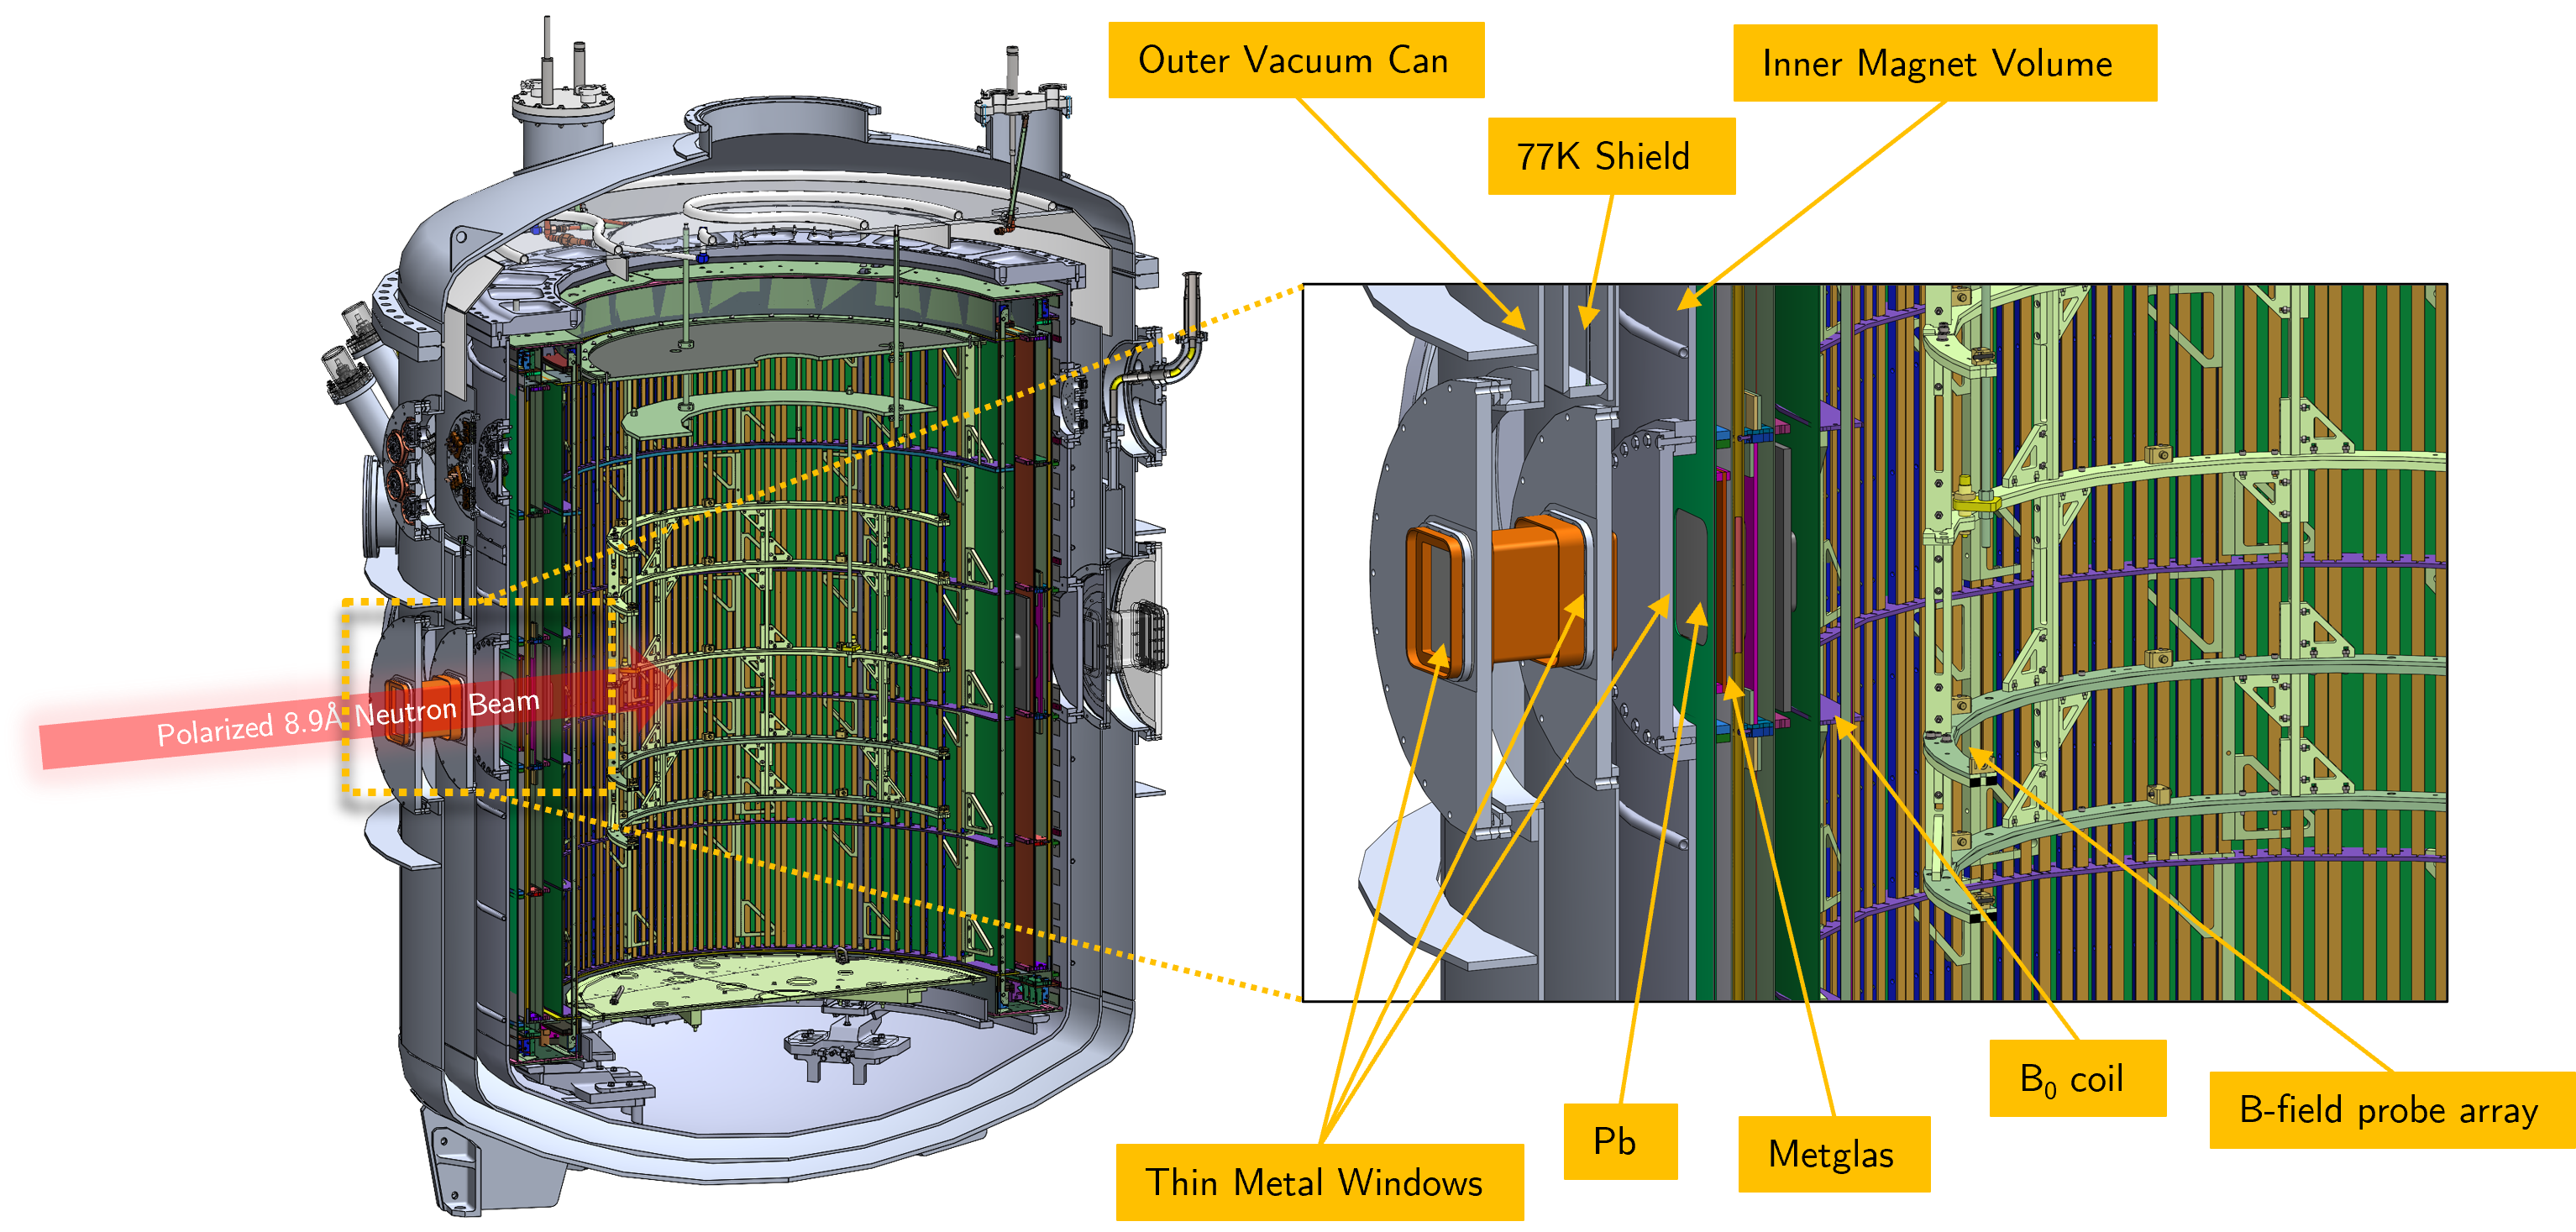
\includegraphics[width=\textwidth]{figures/chapter4-figs/PTtestpicture.png}
    \caption{Overview of proposed neutron polarization and transmission measurement for nEDM@SNS experiment at Beamline 13A. The cryomagnet shown has a vertical height of 3.6 m and a diamter of 3.05 m.}
    \label{fig:PT_pic}
\end{figure}
\clearpage}

The objective of these measurements was to determine the neutron polarization loss and transmission of each of the windows, especially Metglas, in a magnetic field environment similar to the actual nEDM experiment \cite{Ahmed2019}. The primary concern was that the presence of microscopic magnetic domains in the Metglas and the fact that both Pb and the Metglas layers can act as current sheets causing diabatic transition in magnetic field, may lead to depolarization of neutron beam \cite{Ahmed2019}. Polarization measurements through Pb samples for 4~\AA\ neutrons were performed by \cite{Treimer2012} and show strong evidence of magnetic flux trapping, but indicate a reasonable polarization transport. Furthermore, initial testing on Metglas samples were performed at SNS as well as the LENS facility at University of Indiana in 2014 and results indicated relatively minor polarization loss ($\sim$ 10\% polarization loss for 8.9~\AA\ neutrons) \cite{DEFT2014}. Even though these initial measurements indicate a small depolarization, this was attributed to the magnetic fields escaping out of the small foils from the strong applied vertical holding field these measurements were conducted in \cite{DEFT2014, Ahmed2019}. Since simulations of neutron spin orientation undergoing diabatic transition require knowledge of orientation and density of magnetic domains and surface current densities of the materials, it is difficult to determine the grain structure and current densities in Pb and Metglas foils. Therefore, the neutron polarization loss through the beam windows has to measured experimentally in the nEDM cryomagnet's geometry and magnetic field environment. 
%It should be noted that for the final nEDM@SNS experiment, the polarized $^3$He in the measurement cell can be used to recover the expected small neutron polarization loss from the cryostat magnet windows.

This chapter describes the construction of a new beamline, extending from the SNS beamline 13A, to perform the polarization and transmission experiment. Initial neutron flux characterization and dosimtery simulations will be presented. This will be followed by measurements of neutron beam polarization using the in situ polarized $^3$He spin analyzer described in \cref{ch:polHe}. Lastly, the transmission measurements of the nEDM cryomagnet neutron beam windows using small angle neutron scattering beamline at HFIR will be presented as well.

%Prior to the actual nEDM experiment, I propose here to make neutron polarization and transmission measurements at the SNS using Beamline 13A.  The objective is to determine the contribution from each of the materials that the beam passes through, especially Metglas and the superconducting  Pb, the neutron polarization loss in the magnetic field environment of the actual nEDM experiment. The applied magnetic fields and magnetic materials are shown in Fig. 2. While estimates suggest that the polarization losses should be modest it is important to confirm that the presence of magnetic domains in the actual nEDM fields and the changes in B-field between the layers do not introduce significant depolarization. In order to maintain an optimal magnetic field profile, the neutrons pass through both the Pb shield and at least one layer of the ferromagnetic flux-return made from Metglas. The magnetic properties and associated fields from these materials may lead to loss of neutron polarization and we would like to keep any losses to below a few percent. In particular there may be losses between the Pb and Metglas layers, between the Metglas and $B_0$ magnet, as well as losses in passing through the superconducting Pb and through the Metglas.



\section{Neutron Source}

%An overview of the SNS and FnPB 13 is described in detail in ref. \cite{Fomin2015}. This section is a brief recapitulation to provide context for the 2022 BL13A flux measurement and the subsequent neutron polarization and transmission measurements. 

The SNS produces neutrons via spallation by bombarding 1 GeV proton pulses onto a mercury target at a repetition rate of 60 Hz with time-averaged proton power of about 1.7 MW \cite{Fomin2015}. The high energy ($\sim$MeV) neutrons produced get moderated by a liquid hydrogen moderator down to $\sim$meV neutrons. Neutron guides are used to transport neutrons from the ports of the moderators to the individual neutron beamline instruments \cite{Fomin2015}. 

The nEDM@SNS experiment will use polarized monochromatic 8.9~\AA\ neutrons. Therefore, the polarization and transmission measurements described in this experiment will also need to be performed with polarized monochromatic 8.9~\AA\ neutrons. The SNS beamline 13 is equipped with neutron monochromators to provide such neutrons \cite{Fomin2015}. As shown in \cref{fig:BL13A}, 13A utilizes two Alkali-intercalated Graphite crystal monochromators, located 6.5 m downstream from the moderator, to select 8.9~\AA\ neutrons. The first monochromator is a type-I (lattice structure A-B-B-A) potassium intercalated graphite \cite{Mattoni2004, Courtois2011}, consisting of 24 crystals forming a mosaic, each having dimensions 20 mm x 45 mm for a total area of 120 mm x 180 mm \cite{Fomin2015}. It intersects the full beam (100 mm x 120 mm) and reflects neutrons of 8.9~\AA\ with a Bragg angle of 56$\degree$ with respect to the initial beam, as well as $\lambda$/n wavelengths with lower intensity \cite{Fomin2015}. The second monochromator is a type-I rubidium intercalated graphite crystal consisting of 35 crystals, each having dimensions 20 mm x 45 mm for a total area of 140 mm x 225 mm \cite{Fomin2015}. The second monochromator reflects the 8.9~\AA\ beam 113$\degree$ with respect to the initial beam \cite{Fomin2015}. In between the two monochromators are two graphite filters to remove the unwanted $\lambda$/n wavelength neutrons, one oriented to reflect 4.45~\AA\ ($\lambda$/2) and the other 2.97~\AA\ ($\lambda$/3) neutrons \cite{Fomin2015}. The mosaicity of the first monochromator, 3$\degree$, matches the divergence from the upstream guide and the mosaicity from the second monochromator, 5$\degree$, cancels out any first order beam divergence from the first monochromator, allowing the output beam to have the same divergence as the upstream neutron guides \cite{Mattoni2004, Courtois2011}. BL13A continues downstream after the monochromators with an 8 m expanding half ellipsoid neutron guide \cite{Fomin2015}. The beamline opens up inside the beamline 13 shielding enclosure with a rectangular opening cross section of 20 cm x 30 cm \cite{Fomin2015}.

\afterpage{
\begin{figure}
\centering
\includegraphics[width=\textwidth]{figures/chapter4-figs/BL13A_schematic.png}
\caption{A schematic diagram of the monochromatic neutron beamline 13A. The red arrows show the direction of neutron propagation. The label "UCN Guide" referes to beamline 13A.}
\label{fig:BL13A}
\end{figure}
\clearpage}

%\begin{figure}[p]
    %\centering
    %\includegraphics[width=1\textwidth, height=7cm]{beamline13flux.png}
    %\caption{Measured spectrum of neutron flux from beamline 13 (left) \cite{Fomin2015}. Measured spectrum of neutron flux from beamline 13A after the monochromator (right)\cite{Fomin2015}.}
    %\label{fig:flux}
%\end{figure}

\afterpage{
\begin{figure}[p]
    \centering
    \includegraphics[width=\textwidth]{figures/chapter4-figs/frameoverlapmultipulseschedule_2.pdf}
    \caption{Multi-pulse time of flight schedule of neutrons from BL13A as the flight path of neutron increases. The curves represent velocities of 8.9~\AA, 4.45~\AA, 2.97~\AA\ and 2.225~\AA\ neutrons.}
    \label{fig:frameoverlap}
\end{figure}
\clearpage}

The SNS is a pulsed source, emitting neutrons repeatedly at 60 Hz, which allows for the determination of the neutron velocity/wavelength spectrum by measuring the neutron time of flight from the face of the moderator at fixed locations downstream of the moderator. Since there are neutrons of four discrete velocities coming from beamline 13A (444.5 m/s, 888.9 m/s, 1333.9 m/s and 1778 m/s corresponding to 8.9~\AA, 4.45~\AA, 2.97~\AA\ and 2.225~\AA\ respectively), there is possibility of frame overlap of neutrons i.e. 888.9 m/s and 1333.9 m/s neutrons from different pulse frames overlapping with the arrival time of 444.5 m/s neutrons at distances downstream of the moderator. \Cref{fig:frameoverlap} illustrates this effect for BL13A. Frame overlap choppers can be used to isolate desired wavelength of neutrons. These choppers are rotating disks made of neutron-absorbing material with a "pizza-slice" shape cut out. If these choppers are placed at a distance from the moderator and their rotation is phased to the neutron pulse frequency (for e.g. 60Hz), then only neutrons of a particular wavelength (those that arrive when the "pizza-slice" cut is aligned with the beam) will be transmitted. BL13A has one frame overlap chopper at 5.5m from the face of the moderator.

The chopper has an opening angle of $131\degree$ so $ \frac{131\degree}{360\degree} \times \frac{1}{60~\text{Hz}} = 6.06$ ms. This is the the full acceptance width of chopper1 in time of flight. With the chopper opening is 180\degree offset from the guide, the 6.06 ms acceptance window is centered at 8.333 ms, half the time of the 16.67 ms frame. This acceptance will allow neutrons of arrival time within the range of 5.3 ms (8.33 ms-$\frac{6.06 \text{ms}}{2}$) to 11.36 ms (8.333 ms+$\frac{6.06\text{ms}}{2}$). At 5.5m, the arrival times of 2.225~\AA\ (1777 m/s), 2.97~\AA\ (1331 m/s) and 4.45~\AA\ (888 m/s) neutron are 3.1 ms, 4.13 ms and 6.19 ms, respectively. The 2.225~\AA\ (3.1 ms) and 2.97~\AA\ (4.13 ms) miss the acceptance window since 3.1 ms and 4.13 ms are less than 5.3 ms but the 4.45~\AA\ do not, 6.19 ms is greater than 5.3 ms. A time of flight delay needs to be applied, so the chopper can block out the 4.45~\AA\ neutrons, otherwise, they will cause a frame overlap with 8.9~\AA\ neutrons as the flight path of neutron increases. This is shown in \cref{fig:frameoverlap}. With the delay of 5.3 ms, to the no delay center of acceptance of 8.333 ms, the new center of acceptance is at 13.63 ms and the leading edge becomes 10.60 ms(13.63 ms-$\frac{6.06\text{ms}}{2}$) and the lagging edge becomes 16.67 ms (13.63 ms+$\frac{6.06\text{ms}}{2}$) and the 4.45~\AA\ get blocked by the chopper. Now, all of wavelength orders will miss the acceptance set by chopper with a 5.3 ms phase delay, except 8.9~\AA. \Cref{fig:single_pulse_ts_9ang} shows the time of flight pulse schedule with the chopper delay of 5.3 ms and the subsequent wavelength acceptance band of only 8.9~\AA, shown in \cref{fig:trans_9ang}. The reason why the delayed acceptance center is set at 13.36 ms is partly historical as well. The flux characterization measurement of BL-13A in 2010, prior to proposal of this experiment, used a delay of 5.3 ms. The time of flight sequence described above was used to define the full 16.67 ms time of flight frames for the 8.9~\AA\ neutrons, as shown in \cref{fig:multi_pulse_ts_9ang}, for the subsequent measurements.  


\afterpage{
\begin{figure}[p]
    \includegraphics[width=\textwidth]{figures/chapter4-figs/chop_1_single_pulse_ts_9ang.png}
    \caption{Simulated single neutron pulse time of flight schedule for chopper set to 5.3 ms delay to transmit 8.9~\AA\ neutrons. The chopper acceptance is shown in red and the neutron velocity acceptance is shown in blue.}
    \label{fig:single_pulse_ts_9ang}
 \end{figure}
\clearpage}

\afterpage{
\begin{figure}[p]
    \includegraphics[width=\textwidth]{figures/chapter4-figs/chop_1_transmission_9ang.png}
    \caption{Simulated neutron transmission spectrum for chopper set to 5.3 ms delay.}
    \label{fig:trans_9ang}
\end{figure}
\clearpage}

\afterpage{
\begin{figure}[p]
    \includegraphics[width=\textwidth]{figures/chapter4-figs/chop_3_multi_pulse_ts_9ang.png}
    \caption{Simulated multiple neutron pulse time of flight schedule for chopper set to 5.3 ms delay to transmit 8.9~\AA\ neutrons. The chopper acceptance is shown in red and the neutron velocity acceptance is shown in blue.}
    \label{fig:multi_pulse_ts_9ang}
\end{figure}
\clearpage}

\subsection{Beamline 13A Flux Measurement}
   
Prior to the polarization and transmission measurements, the initial neutron flux from the currently existing 13A neutron guide was measured to verify the operation of the monochromators. The previous 13A flux measurement was performed in 2010 \cite{Fomin2015}, therefore, it was crucial to once again verify the health of the monochromators before the polarization and transmission measurement was commenced in 2022. Any decrease in neutron flux will indicate possible degradation of the monochromator's performance and/or any of the beamline neutron guides. %A beam flux reduction to within $10\%$ of the 2010 flux would allow the continuation of the polarization and transmission measurement without a significant negative effect on the measurement's statistical sensitivity. 
This section reports on the 13A flux measurement performed in June 2022. The measurement setup, the results and their implication for the polarization and transmission measurement are discussed.

\subsubsection{Measurement Setup}

A calibrated n-$^3$He low efficiency proportional detector (LND 2232/NIM) was mounted on Al-80/20 support stand and placed after a 1 cm Lithium aperture on the guide exit, giving a total neutron flight distance of 16.04 m from the face of the moderator to the detector. The detector pulse height spectrum was calibrated with a 20 mCi $^{252}$Cf source prior to the measurement. The output from the detector was fed into a pre-amplifier. Both the detector and the pre-amplifier were powered using a NIM crate. The detector had an operating voltage of 800 V. The existing BL13A guide had a 2 inch neutron beam window in front of the 30 cm x 20 cm guide terminal. A lithium aperture with an opening area of 4.28 cm$^2$ was installed on the guide window. This was done to prevent saturating the neutron detector with a high count rate.

\afterpage{
\begin{figure}
\centering
\includegraphics[width=0.5\textwidth]{figures/chapter4-figs/P1_DAQ_Diagram.png}
\caption{Data acquisition setup for June 2022 13A Flux Measurement}
\label{fig:flux_DAQ}
\end{figure}
\clearpage}

The data collection flowchart is shown in \cref{fig:flux_DAQ}. The output from the pre-amplifier was fed into a Single Channel Analyzer (SCA). The SCA had a lower level (LL) of 2 V and a window of 2 V. If the signal from pre-amp fell within the window set between the LL and UL, then the SCA would discriminate on the pre-amplifier analog output and produce a TTL pulse to be sent to the SNS Neutron Event Distributor (nED) DAQ for counting. nED DAQ system was also taking the Real Time Data Link (RTDL) proton beam T$_0$ trigger signal (Event 39) to time synchronize the logic pulses coming from the SCA. The nED DAQ system packed the data into HDF5 data structures and uploaded it to the cloud stream for data analysis.

To start the measurement, the monochromator was lowered into the beam path at the nominal position. This was done via the BL13 FIDO motor control box, which operates the stepper motors that control the crystal's motional degrees of freedom. Only the first linear motor, which vertically translates the monochromator into the beam path, was utilized. There are motors which control the crystal's tilt and rotational degree of freedom but those were kept at their previously optimized settings.

\subsubsection{Analysis and Results}

As shown in \cref{fig:frameoverlap}, there is frame overlap present from $\lambda$ and $\lambda/2$ neutrons at the location of the detector (16.04 m). BL-13A chopper was utilized in this flux measurement to prevent frame overlap. \Cref{fig:chopp_open} shows the time of flight spectrum with the chopper parked at the fully open position. The figure shows the four neutron wavelengths harmonics at the detector location according to their expected time of flight per frame with 100 $\mu$s time bin. The multi-pulse schedule in \cref{fig:frameoverlap} shows that at the detector location, the 8.9~\AA\ and 4.45~\AA, have approximately same arrival time. As shown in \cref{fig:chopp_open}, the dominant peak around 3000 $\mu$s is the 8.9~\AA\ peak and the visible shoulder, around 2000 $\mu$s is the frame overlapping 4.45~\AA\ peak. The peak at around 12000 $\mu$s is the 2.97~\AA\ peak and the low intensity peak at around 8000$\mu$s is the 2.225~\AA\ peak. To separate out the 8.9~\AA\ neutrons from the 4.45~\AA\ neutrons, the chopper was operated at the 5.3 ms phased time delay. \Cref{fig:5.3ms} shows the isolation of the 8.9~\AA\ neutrons from the higher orders with a chopper delay of 5300 $\mu$s and \cref{fig:12.8ms} shows the isolation of the higher orders with a chopper delay of 12800 $\mu$s. The time of flight spectrum in \cref{fig:chopp_run} was analysed to obtain a neutron flux spectrum as a function of wavelength. To do this, first step was to add the 16667$\mu$s frames to the wavelength orders according to their arrival time, as shown in \cref{fig:frameadd}, to obtain an absolute time of flight spectrum. The 8.9~\AA\ neutrons arrive in the third frame, therefore, 33334 $\mu$s (two frames after T$_0$) were added to their arrival time. The 4.45~\AA\ neutrons arrive in the second frame, therefore, 16667 $\mu$s (one frame after T$_0$) were added to their arrival time. The 2.97~\AA\ and 2.225~\AA\ arrive in the first frame.

\afterpage{
\begin{figure}
\centering
  \begin{subfigure}[b]{0.49\textwidth}
    \includegraphics[width=\textwidth]{13A_Chopp_open.pdf}
    \caption{linear-linear axis}
    \label{fig:linlin}
  \end{subfigure}
  \hfill
  \begin{subfigure}[b]{0.49\textwidth}
    \includegraphics[width=\textwidth]{13A_Chopp_open_log.pdf}
    \caption{log-linear axis}
    \label{fig:loglin}
  \end{subfigure}
  \caption{13A time of flight spectrum with chopper fully parked open.}
  \label{fig:chopp_open}
\end{figure}

\begin{figure}
\centering
  \begin{subfigure}[b]{0.49\textwidth}
    \includegraphics[width=\textwidth]{13A_5300microsec__neg25mm_300s.pdf}
    \caption{Chopper phase delay of 5.3 ms to isolate the $\lambda$ neutrons.}
    \label{fig:5.3ms}
  \end{subfigure}
  \hfill
  \begin{subfigure}[b]{0.49\textwidth}
    \includegraphics[width=\textwidth]{13A_12800_695.pdf}
    \caption{Chopper phase delay of 12.8 ms to isolate the $\lambda/2$, $\lambda/3$ and $\lambda/4$ neutrons.}
    \label{fig:12.8ms}
  \end{subfigure}
  \caption{13A time of flight spectrum with chopper running at select phases to isolate the first order peak from the higher orders.}
  \label{fig:chopp_run}
\end{figure}

\begin{figure}
\centering
  \begin{subfigure}[b]{0.49\textwidth}
    \includegraphics[width=\textwidth]{chop_frameadd_2.png}
    \caption{33334 $\mu$s added (two frames after T$_0$) for $\lambda$ neutrons}
    \label{fig:frame2}
  \end{subfigure}
  \hfill
  \begin{subfigure}[b]{0.49\textwidth}
    \includegraphics[width=\textwidth]{chop_frameadd_1.png}
    \caption{16667 $\mu$s added (one frame after T$_0$) for $\lambda/2$ neutrons.}
    \label{fig:frame1}
  \end{subfigure}
  \caption{13A time of flight spectrum with addition of the respective 60Hz frames to get the absolute time of flight in bin width of 100 $\mu$sec.}
  \label{fig:frameadd}
\end{figure}
\clearpage}

The neutron time of flight was converted to neutron wavelength using the relation:
\begin{equation}
    \lambda = \frac{h}{m_n}\frac{t}{L}
\end{equation}
where $\lambda$ is the neutron's wavelength in m, $h$ is the Planck's constant, $m_n$ is the neutron's mass in kg, $t$ is the neutron's time of flight in seconds and $L$ is the neutron's flight distance from the moderator to the detector in meters. This is shown in \cref{fig:framewave}. Prior to the measurement, the efficiency of the neutron detector was measured to be $7.5\times10^{-5} \frac{\text{counts}}{\text{neutrons}}$ at 1~\AA. This efficiency scales linearly with the reciprocal of the neutron velocity at longer neutron wavelengths. This efficiency plus the area of the aperture, 4.28 cm$^2$, were used to convert the histogram in  \cref{fig:neutroneff} from counts per time bin to neutrons per cm$^2$ per time bin in \cref{fig:neutronbinwidth}. The normalization with respect to proton power was done to take into account any accelerator power drop or any proton pulse drops. The charge per proton pulse is measured by the SNS and included in the instrument data acquisition for normalization of neutron flux to the total or per pulse incident protons \cite{Blokland2006}. Given the energy of the pulsed proton beam is 1 GeV, the proton charge was converted to beam power as:
\begin{equation}
    \text{Proton Charge [pC]} \times \frac{1\text{[C]}}{1\times10^{12} \text{[pC]}} \times  \frac{1000.0 \text{[MeV]}}{1 e} \times \frac{1 \text{[J]}}{1 \text{[C $\cdot$ V]}} \times \frac{1 \text{[MW $\cdot$ sec]}}{1 \text{[MJ]}} 
\end{equation}
From this, \cref{fig:neutronbinwidth} was normalized to obtain \cref{fig:neutronpower}, the neutron spectrum per any proton beam power. The neutron flux spectrum as a function of wavelength from 2010 and 2022 measurements is shown in \cref{fig:flux_wavelength}.

\afterpage{
\begin{figure}
    \centering
        \begin{subfigure}[b]{0.475\textwidth}
            \centering
            \includegraphics[width=\textwidth]{chop_stitch.png}
            \caption{13A spectrum normalized to efficiency of neutron detector as well as the area of aperture.}    
            \label{fig:framewave}
        \end{subfigure}
        \hfill
        \begin{subfigure}[b]{0.475\textwidth}  
            \centering 
            \includegraphics[width=\textwidth]{chop_eff_area.png}
            \caption{13A spectrum normalized to efficiency of neutron detector as well as the area of aperture.}   
            \label{fig:neutroneff}
        \end{subfigure}
        \vskip\baselineskip
        \begin{subfigure}[b]{0.475\textwidth}   
            \centering 
            \includegraphics[width=\textwidth]{chop_bin.png}
            \caption{13A spectrum normalized to wavelength bin width.}    
            \label{fig:neutronbinwidth}
        \end{subfigure}
        \hfill
        \begin{subfigure}[b]{0.475\textwidth}   
            \centering 
            \includegraphics[width=\textwidth]{chop_power.png}
            \caption{13A spectrum normalized to the SNS proton beam power.}    
            \label{fig:neutronpower}
        \end{subfigure}

\caption{Normalization procedures for analysis of the BL-13A neutron flux measurement.} 
\label{fig:Fluxanalysis}
\end{figure}
\clearpage}

\afterpage{
\begin{figure}
\centering
  \begin{subfigure}[b]{\textwidth}
    \includegraphics[width=\textwidth]{SpectralNeutronFlux_2010_2022_linlin.pdf}
    \caption{linear-linear axis}
    \label{fig:linlin}
  \end{subfigure}
  \hfill
  \begin{subfigure}[b]{\textwidth}
    \includegraphics[width=\textwidth]{SpectralNeutronFlux_2010_2022_loglin.pdf}
    \caption{log-linear axis}
    \label{fig:loglin}
  \end{subfigure}
  \caption{Measured 13A Flux spectrum as a function of neutron wavelength.}
  \label{fig:flux_wavelength}
\end{figure}
\clearpage}

\subsubsection{Discussion}

\Cref{fig:flux_wavelength} shows that the 13A monochromator is reflecting the same wavelength of neutrons in 2022 as it did in 2010. The exception arises when one compares the peak intensity for the four neutron wavelength orders. The 8.9~\AA\ neutrons, have a lower peak intensity in 2022 from 2010 while the higher order neutrons are showing a high peak intensity in the 2022 measurement as compared to 2010 measurement. This change in intensity for 2022 flux in the different orders of neutron wavelengths can be caused by monochromator crystal orientation misalignment or degradation of the monochromator crystal lattice intercalation spacing or the change in the moderator spectrum as compared to 2010.

Previous measurements with the (LND 2232/NIM) were used to look at the instantaneous count rate for dead time. They indicated minimal dead time at better than 30 kHz instantaneous rate. The apparent dead time is non-paralyzing, with a dead time constant of about 2.6~$\mu$s, leading to negligible loss in counts at the peak.

Despite the increase in intensity of the higher order wavelength neutrons, the first order peak intensity is of primary relevance for the polarization and transmission measurement. During the polarization and transmission measurement, BL13 chopper at 5.5 m from the moderator will need to be operated to eliminate the frame overlap from higher order neutrons and only transmit the 8.9~\AA\ neutrons. Despite the reduced intensity of the 8.9~\AA\ neutrons as measured in 2022, this intensity was still sufficient to provide the expected statistical sensitivity of polarization and transmission measurement. Based on this, it was deemed that the polarization and transmission measurement should proceed forward.    

%\begin{figure}[p]
%\centering
%  \begin{subfigure}[]{0.49\textwidth}
%    \includegraphics[width=\textwidth]{chop_wave2.png}
%    \caption{$\lambda$ neutrons.}
%    \label{fig:wave1}
%  \end{subfigure}
%  \hfill
%  \begin{subfigure}[]{0.49\textwidth}
%    \includegraphics[width=\textwidth]{chop_wave1.png}
%    \caption{$\lambda/2$, $\lambda/3$ and $\lambda/4$ neutrons.}
%    \label{fig:wave2}
%  \end{subfigure}
%  \caption{13A spectrum as a function of neutron wavelength.}
%  \label{fig:wave}
%\end{figure}

%find the bins in the histogram (100 $\mu sec$) should've done non-linear binning

%need to look at instantaneous count rate for dead time

% While you are correct that there's a very low count rate "between the peaks" in your third plot, I suspect that's the end of the frame in the data acquisition system - (was this NED or MCS?). The low rate space is more than 500 us after the peak, and that would be too late - if it was a paralyzing dead time, the apparent rate would (I think) happen more quickly than that.

\subsection{Beamline 13-A Flight Tube}

For the polarization and transmission measurements, a neutron flight tube made of an 10 inch diameter aluminium pipe\footnote{Standard Aluminium pipe is cheap and commercially available.} was constructed to extend the flight path of the monochromatic neutrons from the existing end of the beamline-13A guide, inside the beamline 13 enclosure, to the external building 8713, where the nEDM@SNS cryogenic magnet was set up. This configuration is illustrated in \cref{fig:phase3setup}. The polarization and transmission measurement does not require high statistics and therefore, does not require a high flux beam. It was determined that a neutron flight tube, rather than a neutron guide, would be sufficient for providing neutrons for the PT measurement \footnote{Neutron guides are very expensive and if needed for this measurement, would compound the nEDM@SNS project budget}.

\afterpage{
\begin{figure}
    \centering
    \includegraphics[width=\textwidth]{figures/chapter4-figs/Phase3pic.png}
    \caption{A CAD rendition of the polarization and transmission measurements. The figure shows the flight tube extending from the BL13 enclosure into building 8713, where the cryogenic magnet resides. The upstream and downstream barriers are where the polarimetry components will be setup for the polarization and transmission measurements.}
    \label{fig:phase3setup}
\end{figure}
\clearpage}

\subsubsection{Dose Analysis}

Because the flight tube for the polarization and transmission measurement is an extension beyond the radiological sheilding enclosure of BL13A, dosimetry analysis and measurements were needed in order to identify possible personnel safety and radiation shielding requirements. One of the important steps to commission a new beamline at the SNS is that the dosimetry analysis must indicate that the dose levels are less than the SNS unposted area limit of 0.25 mrem/hr. This analysis then undergoes a SNS facility wide safety review to obtain approval for beam operations. The majority of the radiation during the polarization and transmission measurement comes from the interaction of neutrons with materials along the flight tube geometry. As stated in \cite{Fomin2015}, the BL13A neutron beam is comprised of 8.9$\AA$ neutrons as well as $\lambda/n$ secondary wavelengths from the monochromator. Skimming of the diverging neutron beam is essential for preventing neutron capture on flight tube components. Furthermore, any unavoidable sources of neutron or gamma radiation must be shielded with materials such as lead, borated/lithiated shielding and stainless steel.

The section of the flight tube inside the beamline 13 enclosure was lined with borated shielding material on the inner face of the tube. The shielding material had a high concentration of $^{10}$B for absorption of diverging neutrons from the beam guide, preventing scattering and activation off of the Aluminium pipe and hence, reduce radiation. The flight tube outside the beamline enclosure was also made up of an aluminum pipe with five Li$_2$CO$_3$ skimmers to reduce the beam size to 5 cm in radius as well as prevent the diverging beam from creating radiation.

Monte Carlo computational programs, were utilized to sample and model both beam transport behavior and particle interaction in materials and identify radiation shielding requirements. The initial beam behavior and collimation was modeled using McStas, a Monte Carlo neutron ray-tracing program \cite{Willendrup2020}. By treating the sampled neutrons as ``ray traces" that can reflect and transmit from materials, the beam areal distribution, neutron time of flight and spectral neutron flux were modeled. This was used to optimize the collimation of the beam. All radiation and material interactions modelling was performed with MCNP6, based on the Monte-Carlo method with continuous-energy material cross sections \cite{Goorley2012}. 

A 3D model of the BL-13 enclosure with the polarization and transmission experiment as well as the neighboring Nab experiment were built in the program for accurate radiation transport and shielding calculations. The schematic layout of the proposed neutron polarization and transmission measurement as shown in \cref{fig:phase3setup} was used to develop the geometry in MCNP6 for the dose calculations. The polarizer model was developed in MCNP6 by constructing a box with the polarizer dimensions. The box was filled with boron oxide, the primary absorbing material, with a tuned density to match a 30\% neutron transmission by taking into account the loss mechanisms described above. The “polarizer” is enclosed around its length with steel to mimic the actual encasing of the box. After the polarizer, the neutron beam enters a spin flipper region, which is modeled as a double sided 5 mm thick sheet of Al. The nEDM cryogenic magnet is made of several concentric layers of cryogenic, superconductive, electrically insulating and non-magnetic materials. The neutron beam traverses the nEDM cryomagnet via thin metal beam windows made of Aluminum on the vacuum can and thermal shielding, then superconducting Pb, then low cobalt Metglas and towards the central volume. The 3 outermost layers consist of Al 6061 concentric cylinders which make up the vacuum and thermal shielding. Space between these layers is filled with $10^{-7}$ Torr air and $10^{-1}$ Torr He. The 3D model developed for Nab dosimetry studies was utilized as well to check for effects of the operations of BL13A during the Nab operation and the effects of the operation of Nab experiment towards the 13A polarization and transmission measurement. The main modifications in the Nab 3D model code were the inclusion of the flight tube and the hole in the labyrinth wall to accommodate the flight tube extension.

%This calculation also allowed for the determination of the expected neutron count rate at the end of the flight tube for the polarization and transmission measurement.

In these calculations, 2 MW average proton delivery power was assumed. BL-13A utilizes two Alkali-intercalated graphite monochromators to select 8.9~\AA\ neutrons \cite{Fomin2015}. The measured spectrum of neutrons from the monochromatic BL-13A is shown in \cref{fig:flux_wavelength}. A radially uniform source, a planar disk source with flat areal distribution, of 8.9~\AA\ neutrons was created inside MCNP6 to mimic the beam profile from BL-13A. The source is the average flux density taken from the central portion, radius of 7.62 cm, of the measured 2D beam flux as shown in \cref{fig:beam_image} of \cref{app:beamimg}. Only the neutrons from the central portion will be utilized for the measurement since there will be an initial lithium collimator at the end of the existing guide to capture the neutron flux in the corners in \cref{fig:beam_image} of \cref{app:beamimg}. The initial number of neutrons used in the source was calculated as shown in \cref{eq:MCNPflux}:
\begin{equation}
    7.24\times10^{5}~ \frac{\text{neutrons}}{\text{\AA $\cdot$ cm$^{2}$ $\cdot$ MW $\cdot$ s}} \times 0.5 ~\text{\AA} \times 2.0 ~\text{MW} \times \pi(7.62 ~\text{cm})^{2} = 1.3206\times10^{8} ~\frac{\text{neutrons}}{\text{s}}
    \label{eq:MCNPflux}
\end{equation}
By using the measured spectrum in \cite{Fomin2015}, the energies of the neutrons was set to include the 8.9~\AA\ as well as the $\lambda/2$ and $\lambda/3$ neutrons with spectral ratios of 89.5\%, 13.0\%, 0.5\% and 0.01\% for 8.9~\AA, 4.45~\AA, 2.97~\AA\ and 2.225~\AA, respectively. Beam divergence was included, where neutrons were emerging with a cone angle of $2.52\degree$ perpendicular to the source plane. For the Nab geometry, the source was taken to be the full cold neutron beam spectrum coming from BL-13B. 

%Lithium carbonate will be utilized to collimate the beam out of the flight tube. Li compounds are known to produce fast neutrons of energies up to almost 16 MeV from the n-$^6$Li decay product interaction \cite{Lone}. It is important to check whether these fast neutrons will cause a significant increase in the dose rate. This fast neutron production mechanism is missing from the MCNP6 cross section library, therefore, it has to be modeled as a new source term. To build this source term, first, the number of monochromatic neutrons absorbed in each collimators was calculated by performing an absorption cross section reaction rate tally for each of the collimators in the MCNP6 model. The number of absorbed neutrons was then multiplied by the fast neutron production rate of 1 fast neutron per $10^4$ n-Li capture products (table 2 in \cite{Lone}). These calculations are summarized in Table \ref{tab:fast}. Fig. \ref{fig:fast} shows the energy spectrum of the fast neutrons produced by thermal neutron capture in different Li compounds from \cite{Lone} \& \cite{Santoro}. This energy distribution was used in MCNP6 source term to build five isotropic point sources at the location of each of the Li collimators along the flight tube.

\Cref{fig:doseplot} shows that the calculated dose rate was less then 0.25 mrem/h, the SNS unposted area limit, outside the BL13 enclosure, eliminating the need of extra shielding. The calculations of the radiation fields for the polarization and transmission experiment on BL-13A and worst-case study simulations were also performed. The BL13 shielding enclosure was designed to keep the dose rates outside the enclosure below 0.25 mrem/h for the operation of BL-13A and BL-13B at proton beam power of 2 MW. The enclosure fulfills this requirement since MCNP6 dosimetry calculations show that gamma and neutron dose rates outside the cave walls are less than the 0.25 mrem/hr in all possible scenarios. The calculations also indicated that no area accessible to personnel has a dose rate that exceeds 0.25 mrem/hr. This led us to conclude that it is not necessary to include extra shielding other than the currently existing BL-13 enclosure and flight tube with borated shielding.

\section{Neutron Polarimetry via Polarized ${^3}$He}
\label{sec:PT}

A $^3$He NSF, which utilizes the spin dependent neutron capture on $^3$He, was used as the neutron polarization analyzer to measure the polarization of neutron beam traversing through the cryomagnet. The polarization of a neutron beam can be determined from transmission measurements through a $^3$He cell \cite{Greene1995, Musgrave2018}. $^3$He polarization and the physical properties of the $^3$He cell do not need to be known to determine the neutron polarization \cite{Greene1995}.

\begin{landscape}
\thispagestyle{mylandscape}
 \begin{figure}
    \centering
    \begin{subfigure}[b]{1.2\textwidth}
    \includegraphics[width=1\linewidth]{fig3.png}
    \caption{}
    \label{fig:gammadose} 
    \end{subfigure}
    \begin{subfigure}[b]{1.2\textwidth}
    \includegraphics[width=1\linewidth]{fig4.png}
    \caption{}
    \label{fig:neutrondose}
    \end{subfigure}
\caption{Dose rate heat maps of the 3D model of proposed neutron polarization transmission measurement at BL-13A simulated in MCNP6. The figure shows a top down view of the the extension of BL-13A via flight tubes towards the SNS building 8713, the Neutron polarizer and the nEDM cryogenic magnet. The gamma ray dose rate is shown in (a) and the neutron dose rate is shown in (b). The units of dose rate are in [rem/hr] with the color red set to be above the SNS unposted area limit of $2.5\times10^{-4}$ rem/hr.}
\label{fig:doseplot}
\end{figure}   
\end{landscape}

As previously described in \cref{ch:polHe}, the transmission of neutrons through a 3He cell is determined from:
\begin{equation}\label{eq:tzero}
    T_0=T_e e^{-\zeta}
\end{equation} 
where $\zeta$ is the opacity defined in \cref{eq:opacity}. The transmission of spin up ($\uparrow$) and spin down ($\downarrow$) neutrons through a polarized $^3$He analyzer with polarization $P_{He}$ (by making initial neutron polarization implicit) becomes:
\begin{equation}
    T_\uparrow = N_0\frac{\left(1+P_n\right)}{2}e^{-\zeta (1-P_{He})}
\end{equation}
\begin{equation}
    T_\downarrow = N_0\frac{\left(1-P_n\right)}{2}e^{-\zeta (1+P_{He})}
\end{equation}
Hence the total transmission of a polarized neutron beam through polarized $^3$He analyzer becomes:
\begin{equation}\label{eq:t}
    T = T_\uparrow + T_\downarrow = N_0e^{-\zeta}\cosh{\left(\zeta P_{He}\right)}\left[1+P_n\tanh{\left(\zeta P_{He}\right)}\right]
\end{equation}
To obtain the other spin state, a neutron spin flipper is used to rotate the spins by $\pi$ radians with efficiency $\epsilon_{sf}\leq1$. The magnitude of the neutron polarization becomes $(1-2\epsilon_{sf})P_n$: 
\begin{equation}\label{eq:tsf}
    T_{sf} = N_0e^{-\zeta}\cosh{\left(\zeta P_{He}\right)}\left[1+\left(1-2\epsilon_{sf}\right)P_n\tanh{\left(\zeta P_{He}\right)}\right]
\end{equation}

The neutron polarization, $P_n$ can be determined from three transmission measurements, neutron transmission through unpolarized $^3$He ($T_0$ in \cref{eq:tzero} ) and transmission through polarized $^3$He for both neutron spin states ($T$ in \cref{eq:t} and $T_{sf}$ in \cref{eq:tsf}). The ratio of the neutron transmission through polarized and unpolarized $^3$He eliminates various non-ideal systematic errors arising from the neutron detector. If we define the ratio of $T$ with $T_0$ as $R$, the ratio of $T_{sf}$ with $T_0$ as $R_{sf}$:
\begin{equation}\label{eq:R}
    R = \frac{T}{T_0} = \cosh{\left(\zeta P_{He}\right)}\left[1+P_n\tanh{\left(\zeta P_{He}\right)}\right]
\end{equation}
\begin{equation}\label{eq:Rsf}
    R_{sf} = \frac{T_{sf}}{T_0} = \cosh{\left(\zeta P_{He}\right)}\left[1+\left(1-2\epsilon_{sf}\right)P_n\tanh{\left(\zeta P_{He}\right)}\right]
\end{equation}
By using the trigonometric identity, $1 - \tanh^2{x} = \sech^2{x}$, and substituting in \cref{eq:R} and \cref{eq:Rsf} to solve for $\cosh{\zeta}$:
\begin{equation}
    \cosh{\zeta} = \frac{1}{2\epsilon_{sf}}\left[R_{sf}-(1-2\epsilon_{sf})R\right]
\end{equation}
This result allows \cref{eq:R} and \cref{eq:Rsf} to become:
\begin{equation}\label{eq:R_nocosh}
    R = \frac{1}{2\epsilon_{sf}}\left[R_{sf}-(1-2\epsilon_{sf})R\right] - P_n\sqrt{\left[\frac{1}{2\epsilon_{sf}}\left[R_{sf}-\left(1-2\epsilon_{sf}\right)R\right]\right]^2 -1}
\end{equation}
\begin{equation}\label{eq:Rsf_nocosh}
    R_{sf} = \frac{1}{2\epsilon_{sf}}\left[R_{sf}-\left(1-2\epsilon_{sf}\right)R\right] - \left(1-2\epsilon_{sf}\right)P_n\sqrt{\left[\frac{1}{2\epsilon_{sf}}\left[R_{sf}-\left(1-2\epsilon_{sf}\right)R\right]\right]^2 -1}
\end{equation}
From \cref{eq:R_nocosh} and \cref{eq:Rsf_nocosh}, the polarization of neutrons can be determined simply as function of neutron transmission ratios and spin flipper efficiency $\epsilon_{sf}$:
\begin{equation} \label{eq:polarization}
P_n=\frac{R-R_{sf}}{\sqrt{\left[\left(2\epsilon_{sf}-1\right)R+R_{sf}\right]^{2}-4\epsilon_{sf}^2}}
\end{equation}

\subsection{Efficiency of spin flipper}

The spin-flip efficiency, $\epsilon_{sf}$ , can be determined from four transmission measurements: two with the initial neutron spin state, $T$ and $T^{AFP}$, and another two with the neutrons spin flipped, $T_{sf}$ and $T^{AFP}_{sr}$ for both $^3$He polarization states. AFP corresponds to transmission measurements where the $^3$He polarization was reversed by adiabatic fast passage (AFP). Four transmission measurements give the ratios $R$ and $R_{sf}$:
\begin{equation}
    \frac{T^{AFP}-T}{T^{AFP}+T} = P_n\tanh{\left(\zeta P_{He}\right)} = R
\end{equation}
\begin{equation}
    \frac{T^{AFP}_{sr}-T_{sf}}{T^{AFP}_{sr}+T_{sf}} = \left(1-2\epsilon_{sf}\right)P_n\tanh{\left(\zeta P_{He}\right)} = R_{sf}
\end{equation}
The spin flipper efficiency can be calculated from these ratios as:
\begin{equation}
\begin{split}
    \epsilon_{sf} & = \frac{1}{2} \left( 1 - \frac{R_{sf}}{R}  \right) \\
    & =\frac{1}{2} \left(1-\frac{\frac{T^{AFP}_{sr}-T_{sf}}{T^{AFP}_{sr}+T_{sf}}}{\frac{T^{AFP}-T}{T^{AFP}+T}}\right) 
\end{split}
\end{equation}

An important note needs to be made here. To polarize the neutron, a neutron polarizing device is employed. Since the polarization of the beam is defined based on the guiding magnetic field, guiding magnetic field components have to be used to maintain the polarization and provide spin transport from the polarizing device to the analyzing device. It is also important to characterize the spin flipped state, so a spin flipper is also utilized. Therefore, the neutron beam polarization is actually the product of the spin transport efficiency, $\epsilon_{ST}$, the spin flipper efficiency, $\epsilon_{SF}$, the spin polarizing power of the neutron polarizer, $P_{n}$, and the spin analyzing power, $P^{He}_{n}$, of the spin analyzer as:
\begin{equation}
    \epsilon_{ST} \cdot \epsilon_{SF} \cdot P_{n} \cdot P^{He}_{n} = \frac{R_{\uparrow}-R_{\downarrow}}{R_{\uparrow}+R_{\downarrow}}
\end{equation}
Since the beam polarization is set by the neutron polarizer and defined by the spin transport, $P_{n}$ and $\epsilon_{ST}$ cannot separated. Therefore, the beam polarization is defined as:
\begin{equation}
    \epsilon_{ST} \cdot P_{n} \rightarrow P_{n} = \frac {1}{ \epsilon_{SF} \cdot P^{He}_{n} } \left( \frac{R_{\uparrow} - R_{\downarrow}}{R_{\uparrow}+R_{\downarrow}}  \right) =  \frac{R_{\uparrow} - R_{\downarrow}}{ \sqrt{ \left(\left(2\epsilon_{sf}-1\right)R_\uparrow + R_\downarrow \right)^2 - 4\epsilon_{SF}^2 }  } 
\end{equation}
where $ \epsilon_{SF} = \frac{1}{2} \left(  1 - \frac{R_\downarrow}{R_\uparrow}     \right) $, is the efficiency of the spin flipper used to flip $R_\uparrow$ to $R_\downarrow$.

\section{Experimental Setup and Measurement Scheme}

This section will cover the experimental setup for the different configurations used to measure the transmission and polarization loss from the cryomagnet. The first configuration was to measure the neutron transmission loss from the cryomagnet. This setup is illustrated in \cref{fig:trans_setup}. The objective here is to measure the neutron beam intensity before the cryomagnet and then after the cryomagnet. The ratio of the transmissions will determine the fraction of neutron beam lost due to the presence of the cryomagnet. First, the neutron beam was defined based on the two $^6$Li apertures with 2 cm by 2 cm opening. The placement and opening of these apertures lock in the beam cross sectional area going into the cryomagnet. To measure the neutron intensity before the cryomagnet, the neutron detector was placed upstream of the cryomagnet, as shown in \cref{fig:upstream_trans}. To measure the neutron intensity after the cryomagnet, the same neutron detector was placed downstream of the cryomagnet as shown in \cref{fig:downstream_trans}. It is crucial for the apertures to ensure that the neutrons detected in the upstream configuration are the same neutrons that traverse the cryomagnet and are detected at the downstream configuration.

\afterpage{
\begin{figure}
\centering
  \begin{subfigure}[]{\textwidth}
    \includegraphics[width=\textwidth]{figures/chapter4-figs/upstream_trans.png}
    \caption{}
    \label{fig:upstream_trans}
  \end{subfigure}
  \hfill
  \begin{subfigure}[]{\textwidth}
    \includegraphics[width=\textwidth]{figures/chapter4-figs/downstream_trans.png}
    \caption{}
    \label{fig:downstream_trans}
  \end{subfigure}
  \caption{A schematic setup to measure the transmission loss of neutron beam through the nEDM cryomagnet by measuring the initial beam in (a) and after beam in (b). Here the component "Source" refers to the neutron flight tube. The blue dotted arrow represents the neutron beam.}
  \label{fig:trans_setup}
\end{figure}
\clearpage}

\afterpage{
\begin{figure}
\centering
  \begin{subfigure}[]{\textwidth}
    \includegraphics[width=\textwidth]{figures/chapter4-figs/upstream_polarimetry.png}
    \caption{}
    \label{fig:upstream_pol}
  \end{subfigure}
  \hfill
  \begin{subfigure}[]{\textwidth}
    \includegraphics[width=\textwidth]{figures/chapter4-figs/downstream_polarimetry.png}
    \caption{}
    \label{fig:downstream_pol}
  \end{subfigure}
  \caption{A schematic setup for the (a) upstream polarimetry measurement and (b) downstream polarimetry measurement. Here the component "Source" refers to the neutron polarizer and neutron spin flipper. The blue dotted arrow represents the polarized neutron beam.}
  \label{fig:polarimetry_setup}
\end{figure}
\clearpage}

The second setup was to measure the neutron polarization loss from the cryomagnet via transmission of neutrons through the $^3$He analyzer for neutron polarimetry based on \cref{eq:polarization}. \Cref{fig:polarimetry_setup} illustrates the setup used to measure the polarization of the neutron beam before and after the cryomagnet. The difference between the measured polarization upstream of the cryomagnet and downstream of the cryomagnet will be used to determine the contribution of the cryomagnet windows and its magnetic fields to neutron polarization loss. The initial beam emerging from the flight tube is unpolarized, therefore, a neutron polarizer is placed to polarize the neutron beam. Then a neutron spin flipper is placed after the polarizer. The flipper is placed to account for its contribution towards beam intensity loss as the beam traverses through it but it is only activated when the measurement configuration call for it. For the entire neutron polarimetry run, the neutron detector was placed downstream of the cryomagnet. The neutron beam was defined by two $^6$Li apertures with 2 cm by 2 cm opening, first one placed after the spin flipper and the second one placed right before the neutron detector. The placement and opening of these apertures ensures that polarized neutrons are going the $^3$He neutron spin analyzer. A caveat of this measurement scheme is the assumption that the neutrons were polarized uniformly along the entire phase space of the defined neutron beam. To measure the neutron polarization before the cryomagnet, the neutron spin analyzer was placed upstream of the cryomagnet, as shown in \cref{fig:upstream_pol}. To measure the  neutron polarization after the cryomagnet, the neutron spin analyzer was placed downstream of the cryomagnet as shown in \cref{fig:downstream_pol}. To measure the neutron beam polarization upstream and downstream, neutron beam polarization and neutron spin analyzer configurations as shown in \cref{fig:pol_scheme} were used. These configuration are as follows:
\begin{enumerate}
    \item First, as shown \cref{fig:directbeam}, the transmission of the polarized neutron beam without the $^3$He neutron spin analyzer was measured.
    \item Second, as shown \cref{fig:unpolcell}, the transmission of the polarized neutron beam with an unpolarized $^3$He neutron spin analyzer was measured.
    \item Third, as shown \cref{fig:polbeam}, the transmission of the polarized neutron beam with a polarized $^3$He neutron spin analyzer (the beam polarization is parallel relative to the polarized $^3$He) was measured. This is called the high transmission spin state of the spin analyzer.
    \item Fourth, as shown \cref{fig:sfbeam_polcell}, the transmission of the spin flipped neutron beam with a polarized $^3$He neutron spin analyzer (the beam polarization is anti-parallel relative to the polarized $^3$He) was measured. The neutron beam spin was flipped using a neutron spin flipper. This measurement is called the low transmission spin state of the spin analyzer.
    \item Fifth, as shown \cref{fig:polbeam_afpcell}, the transmission of the polarized neutron beam with an anti-polarized $^3$He neutron spin analyzer was measured. The polarized $^3$He was inverted using the AFP technique described in \cref{ch:polHe}
    \item Sixth, as shown \cref{fig:sfbeam_afpcell}, the transmission of the spin flipped neutron beam with an anti-polarized $^3$He neutron spin analyzer was measured.
\end{enumerate}
The transmission of polarized neutrons through the neutron spin analyzer based on these above configurations will determine the relevant transmission ratios needed to extract the neutron beam polarization using \cref{eq:polarization}. The neutron polarizing instruments and the neutron detector are described in detail the following sections.



\afterpage{
\begin{figure}
    \centering
    \begin{subfigure}[b]{0.6\linewidth}
        \includegraphics[width=\linewidth, height=2.5cm]{noanalyzer.png}
    \caption{$N_0$}
    \label{fig:directbeam}
    \end{subfigure}
    \hfil
    \begin{subfigure}[b]{0.75\linewidth}
        \includegraphics[width=\linewidth, height=2.5cm]{figures/chapter4-figs/unpolarizedcell.png}
    \caption{$T_0$}
    \label{fig:unpolcell}
    \end{subfigure}

    \begin{subfigure}[b]{0.75\linewidth}
        \includegraphics[width=\linewidth, height=2.5cm]{figures/chapter4-figs/polbeam.png}
    \caption{$T$}
    \label{fig:polbeam}
    \end{subfigure}
    \hfil
    \begin{subfigure}[b]{0.75\linewidth}
        \includegraphics[width=\linewidth, height=2.5cm]{figures/chapter4-figs/sfbeam_polcell.png}
    \caption{$T_{SF}$}
    \label{fig:sfbeam_polcell}
    \end{subfigure}

    \begin{subfigure}[b]{0.75\linewidth}
        \includegraphics[width=\linewidth, height=2.5cm]{figures/chapter4-figs/polbeam_afpcell.png}
    \caption{$T^{AFP}$}
    \label{fig:polbeam_afpcell}
    \end{subfigure}
    \hfil
    \begin{subfigure}[b]{0.75\linewidth}
        \includegraphics[width=\linewidth, height=2.5cm]{figures/chapter4-figs/sfbeam_afpcell.png}
    \caption{$T^{AFP}_{SF}$}
    \label{fig:sfbeam_afpcell}
    \end{subfigure}
\caption{Transmission of polarized neutrons through $^3$He cell for neutron polarimetry.}
\label{fig:pol_scheme}
\end{figure}
\clearpage}


\subsection{Neutron Polarizer}

Due to their nuclear potential and the magnetic moment, neutrons are capable of coherent nuclear scattering as well as magnetic scattering of off materials or a mirror coated with a magnetizable layer \cite{Hughes1951}. The nuclear and magnetic scattering lengths, $a_{nuc}$ and $a_{mag}$, respectively, of these mirrors make up the neutron’s index of refraction , $n$, as:
\begin{equation}
    n \simeq 1- \frac{N \lambda^2}{2 \pi} \left( a_{nuc} \pm a_{mag} \right)
\end{equation}
where $N$ is the atomic number density of mirror and $\lambda$ is the incident neutron wavelength. The mirror is placed in a polarization defining magnetic field from which the difference in the magnetic scattering length arises, leading to a reflection/refraction of neutron spin states \cite{Hughes1951, Scharpf1991}. From Snell's law, the critical angle of the spin dependent neutron reflection/refraction can be written as:
\begin{equation}
    \theta_c = \lambda \sqrt{  \frac{N}{\pi}  \left( a_{nuc} \pm a_{mag} \right) }
    \label{eq:critangle}
\end{equation}
Between the two critical angles formed by \cref{eq:critangle}, the neutrons are effectively polarized, where one spin state is reflected and the other is refracted i.e. transmitted through the mirror \cite{Hughes1951, Scharpf1991}. 

The critical angle range can be extended to allow for large angle of incidence acceptance and polychromatic neutron beams by employing "super mirrors" \cite{Mezei1976, Mezei1977}. The super mirror is composed of multiple layers of non-magnetic/magnetic bi-layer mirrors. By layering a magnetic material with large nuclear and magnetic scattering lengths with a nonmagnetic material with a scattering length close to zero, a neutron polarizing mirror is created that is highly reflective for one spin state. If the nuclear and magnetic scattering lengths of the magnetic material are approximately equal, the scattering length is constant and close to zero for the other spin state. The supermirror multi-layers vary in thickness to create virtual lattices of different spacings, allowing for multiple Bragg reflections for multiple wavelengths of neutrons, effectively increasing the supermirror’s reflectivity beyond the critical angle of the magnetized bi-layers \cite{Mezei1976, Mezei1977}. This makes super mirrors useful for polarizing a broad range of neutron wavelengths. The reflectivity is constant for incidence angles less than the critical angle of the magnetic material. Beyond that, the reflectivity declines until the effective critical angle created by the super mirrors. This effective critical angle is characterized by the ``$m$" factor. The $m$ factor is relative to the neutron reflection off a $^{58}$Ni surface, since $^{58}$Ni has the largest single layer critical angle. Thus, the $m$ factor indicates that the supermirror’s critical angle is a factor of $m$ greater than a smooth $^{58}$Ni surface and can be found from:
\begin{equation}
   \theta_{c,smp}[mrad] =1.73 \left[\frac{mrad}{\AA} \right] \cdot \lambda [\AA] \cdot m 
\end{equation}
 
This polarization and transmission measurement utilized a 40~cm long and 10~cm $\times$ 12~cm supermirror polarizer, composed of 45 panes (each 0.3~mm thick) of borofloat glass with Fe/Si coating of m=3 \cite{Balascuta2012}, to polarize the monochromatic neutron beam. The panes have a 9.6 cm radius of curvature to (i) accept the divergence of the incoming beam and (ii) to ensure the incoming neutrons experience at least a single bounce and hence, polarize before emerging from the instrument. Iron is used for the ferro-magnetized layers, and Silicon forms the magnetically transparent layers due to it's small neutron scattering cross section \cite{Balascuta2012, Schanzer2016}. Permanent magnets envelop the supermirror polarizer and create a magnetic field of about 380 Gauss to saturate the magnetization of the Fe layers \cite{Balascuta2012}. The magnetization Fe layers create the magnetic scattering length for the supermirror polarizer \cite{Schanzer2016, Mezei1976}. The neutrons with angle of incidence greater than the $\theta_{c,smp}$ refract into the borofloat substrate and get absorbed while the neutrons with glancing angle reflection emerge from the SMP as polarized \cite{Balascuta2012}. Since the polarization from the supermirror depends on the wavelength and angle of incident of the neutron beam and is time-independent, the polarization of the neutron beam does not have to be continuously measured for each neutron pulse. %About 95 $\%$ polarization is expected from the supermirror polarizer for neutron wavelengths 8.9 \AA.

The controlling parameter of the supermirror polarizer is its alignment with the neutron beam. A rough translational as well as rotational alignment was performed to ensure the logitudinal axis of the polarizer was parallel to the beam axis of the flight tube. The important rotation angle to consider is the rotation about the yaw axis at the pivot of the upstream end of the polarizer with respect to the beam. McStas simulations of the polarizer, as shown in \cref{fig:mcstas_pol_sweep}, show the that maximum transmission of neutrons from the polarizer occurs the yaw angle of $0 \degree$. The polarizer was set to this angle for all the measurements taken. Technically, the figure to tune the ideal yaw angle of the polarizer is $P \cdot T^2$, where, $P$, is the neutron polarization and, $T$, is the neutron transmission. However, it can be argued because the design of the polarizer prohibits line of sight neutrons, all neutrons exiting the polarizer have had a chance to bounce of the supermirror surface and hence, become polarized. Therefore, it was sufficient to use the maximum transmission setting as the ideal.  

\afterpage{
\begin{figure}
    \centering
    \includegraphics[width=\textwidth]{figures/chapter4-figs/pol_rot.png}
    \caption{McStas simulated neutron intensity transmitted from the supermirror polarizer as a function of the yaw angle about the vertical axis.}
    \label{fig:mcstas_pol_sweep}
\end{figure}
\clearpage}

%For most materials, which possess neutron refractive indices slightly smaller than 1, neutrons will undergo total external reflection from the optical potential $V_{opt}$ of the medium if their angle of incidence is below a critical angle ${\theta}_c$, determined by the material density, the neutron coherent scattering length $b_{coh}$, and the neutron wavelength.
%\begin{equation}
    %\theta_c=\lambda\sqrt{\frac{Nb_{coh}}{\pi}}
%\end{equation}
%where reflection of neutrons with wavelengths beyond the critical angle is achieved by layering materials with different refractive indices to simulate a virtual one-dimensional lattice of spacing d for Bragg diffraction [7].
%\begin{equation}
 %   n\lambda=2d\sin{\theta}
%\end{equation}

%A neutron entering a medium will interact with its nuclear potential. The low energy neutrons being utilized for this experiment have kinetic energies of $\sim$1 meV, ($\lambda_n \sim nm$) which is much less than the typical nuclear potential of tens of MeV with only a couple of femtometer range. This means that wavelength of these low energy neutrons is much longer compared to the range of the nuclear potential. If we assume that the neutron experiences a change of energy equivalent to the effective potential of the entire medium, $\langle V \rangle$, the index of refraction can be written as:

\subsection{Spin Flipper}

The polarization direction of the neutron beam is defined by the guiding magnetic field. This guiding magnetic field can be adiabatically reoriented and hence, in the lab frame, the polarization of the beam with respect to the guide field will remain constant, following the adiabatically reoriented guiding magnetic field. However, for a diabatic reorientation of the guiding magnetic field, the polarization will not follow the sudden change in the guiding magnetic field direction; instead the neutron beam will preserve its initial state, and precess about the new guiding magnetic field direction. These adiabatic and diabatic rotations of the guiding magnetic field enable the neutron beam polarization to be effectively inverted or flipped with respect to the guiding magnetic field. 

In order to determine the neutron beam polarization, the neutron spin state anti parallel to the guide field also has to be characterized, since polarization is defined as the contrast in parallel and anti-parallel spin states. In order to  measure the transmission of spin flipped neutrons through the analyzer cell, $T_{sf}$, a neutron spin flipper is used to flip the neutron spin to the opposite spin state. Since this experiment is dealing with monochromatic neutrons, i.e. neutrons of fixed velocity, diabatic spin flippers are appropriate. A Mezei coil is a type of a diabatic flipper that was built for this purpose \cite{Mezei1972, Hayter1978}. This flipper consists of a rectangular solenoid of fixed thickness, which provides a strong DC magnetic field perpendicular the guide field to induce a torque on the magnetic moment of the polarized neutrons of fixed velocity for $n\pi$ radians spin flips, where n is an odd integer. The strength of the perpendicular flipper field, $B_{flipper}$, can be found by:
\begin{equation}
    \gamma_n B_{flipper} = \frac{\phi v_n}{ d}
\end{equation}
where $\phi$ is the spin rotation angle, $v_n$ is the velocity of the neutrons, $d$ is the thickness of the coil and $\gamma_n$ is the neutron's gyromagnetic ratio.

A Mezei spin flipper was constructed to be used for this experiment, as shown in \cref{fig:Mezei-built}. The flipper consists of four major parts: (i) The inner most coil, made of Aluminum ribbon wire, is the spin flip coil responsible for providing the perpendicular guide field, (ii) The outer frame of the flipper is responsible for providing a continuous guide field. Permanent magnets are placed on the sides and the iron yokes provide a homogeneous field return, (iii) the outer most coil, also made of aluminum ribbon wire, cancels the guide field, so that the neutron effectively precesses about the perpendicular field created by (i). The neutron beam goes through middle of the coil. There are two pairs of orthogonal shim coils that can provide a cancelling field in the beam axis, if needed.

\afterpage{
\begin{figure}
    \centering
    \includegraphics[width=\textwidth]{figures/chapter4-figs/Flipper_picture.png}
    \caption{The Mezei spin flipper built for the neutron polarimetry and transmission experiment.}
    \label{fig:Mezei-built}
\end{figure}
\clearpage}

\afterpage{
\begin{figure}
    \centering
    \includegraphics[width=\textwidth]{figures/chapter4-figs/HB2D_Sbender.pdf}
    \caption{4.2~\AA\ neutron count rate while sweeping the S-bender angle.}
    \label{fig:benderopt_HFIR}
\end{figure}
\clearpage}

\afterpage{
\begin{figure}
    \centering
    \includegraphics[width=\textwidth]{figures/chapter4-figs/HB2D_SFtest.pdf}
    \caption{4.2~\AA\ neutron count rate at 2.6$\degree$ S-bender angle while sweeping the flipper coil current for different guide field cancellation coil currents.}
    \label{fig:SFeff_HFIR}
\end{figure}
\clearpage}

This flipper was tested at the HFIR neutron instrument developed beamline (HB2D), which is designed for testing prototypes of neutron polarizing devices \cite{Crow2016}. HB2D consists of a monochromatic 4.2~\AA\ neutron beam, a V-cavity neutron polarizer, a S-shaped bender polarizer \footnote{See \href{https://www.swissneutronics.ch/}{SwissNeutronics} for more information on the different types of neutron devices.} for neutron spin analysis and a $^3$He detector for neutron counting \cite{Crow2016}. The test included characterization of the flipping ratio and hence, the flipping efficiency of Mezei flipper based on the methodology described in \cite{Li2020, Dadisman2020}, where RF and adiabatic neutron spin flippers were characterized similarly at HB2D. The transmission measurements of polarized neutrons through the Mezei spin flipper as a function of flipper coil current were preformed. First, the S-shaped bender polarized neutron analyzer was optimized by measuring the transmission of polarized neutrons as a function of the angle of incidence of the incident neutron beam. The results are shown in \cref{fig:benderopt_HFIR}. The S-bender analyzer was set at the optimum angle of $2.6\degree$ for the flipper testing. Next, the flipper was optimized by varying the spin flipper coil current for different current values of the guide field cancelling coil. \cref{fig:SFeff_HFIR} shows the the high transmission spin state neutrons (based on the S-bender spin selection preference) and low transmission spin state neutrons as a sweep of the spin flipper current coil. The best flipping ratio, $f=\frac{N_{high}}{N_{low}}$, or the spin contrast was measured as 26.74 at 9.8 A current in the spin flipper coil. The polarizing efficiency of the spin flipper, $\frac{f-1}{f+1}$, at 4.2~\AA\ was measured as:
\begin{equation}
    \epsilon_{SF} = 0.93 \pm 0.06_{stat}
\end{equation}
This measurement was repeated for 8.9~\AA\ neutrons at beamline 13A. First, the outer coil current was swept with no spin flip coil current to find the lowest transmission of neutrons. This occurred at an outer coil current of -17.5 A, indicating that at this current value, the outer coil was maximally cancelling out the guide field and causing a diabatic transmission. Next, the spin flipper coil current was swept to find the maximum flipping ratio. The results are shown in \cref{fig:SFeff_SNS}, where the maximum flipping ratio of $\approx1.7$ took place at -5.8 A. The flipping efficiency at 8.9~\AA\ was measured to be:
\begin{equation}
    \epsilon_{SF} = 0.92 \pm 0.03_{stat}
\end{equation}
Two important observation should be noted here. First, both \cref{fig:SFeff_HFIR} and \cref{fig:SFeff_SNS} show that that spin flipping contrast is more robust at higher currents i.e. large $B_{flipper}$, meaning the effective magnetic field from the flipper coils becomes more and more perpendicular. Therefore, it is more efficient to use $3\pi, 5\pi, ...$ and beyond spin turns for more robust spin flips. Second, the fringe pattern observed for 4.2~\AA\ neutrons in \cref{fig:SFeff_HFIR} is twice as broad as the pattern observed for 8.9~\AA\ neutrons in \cref{fig:SFeff_SNS}. This is because 4.2~\AA\ are faster than 8.9~\AA\ neutrons and therefore, a high $B_{flipper}$ field i.e. high coil current, is needed to provide a torque to flip their polarization. 

\afterpage{
\begin{figure}
    \centering
    \includegraphics[width=\textwidth]{figures/chapter4-figs/SNS_SFtest.pdf}
    \caption{8.9~\AA\ neutron count rate while sweeping the flipper coil current for the guide field cancellation coil current of -17.5 A.}
    \label{fig:SFeff_SNS}
\end{figure}
\clearpage}

\subsection{Neutron Spin Transport}

To describe the polarization of the neutron beam, a semi-classical picture is used, where a neutron with a magnetic moment aligned with the spin angular momentum vector, $\Vec{S}$, precesses in a magnetic field, $\Vec{B}$, with an angular frequency, $\omega_L$, called Larmor frequency defined as $\omega_L$ = $\gamma_n \Vec{B}$. The rate of change of the angular rotation of the spin (under cartesian coordinates) is given by the Bloch equation\cite{Bloch1946}:
\begin{equation}
    \frac{d\Vec{S}(t)}{dt} = \gamma_n \left( \Vec{S}(t) \times \Vec{B}(t)  \right)
    \label{eq:Bloch}
\end{equation}
which when written in terms of all of the components of $\Vec{S}(t)$ and $\Vec{B}(t)$ becomes:
\begin{align}
\begin{split}
    \frac{dS_x(t)}{dt} &= \gamma_n \left( S_y(t) B_z(t) - S_z(t) B_y(t) \right) \\
    \frac{dS_y(t)}{dt} &= \gamma_n \left( S_z(t) B_x(t) - S_x(t) B_z(t) \right) \\
    \frac{dS_z(t)}{dt} &= \gamma_n \left( S_x(t) B_y(t) - S_y(t) B_x(t) \right)
    \label{eq:Blochcomp}
\end{split}
\end{align}
The time evolution of \cref{eq:Blochcomp} can be written in terms of the ratio of the distance travelled by the neutron in the guiding magnetic field, $l$, to the velocity of the neutron, $v_n$. This means that, \cref{eq:Blochcomp} can be used to trace the dynamics of the spin vector components of a neutron propagating through an arbitrary magnetic field environment over the course of the experimental setup. Using this technique, the spin transport for the monochromatic 8.9~\AA\ neutrons, i.e. velocity of 444 m/s, was simulated based on the magnetic fields created by the guide field and polarimetry components of the experiment.

\afterpage{
\begin{figure}
    \centering
    \includegraphics[width=1\textwidth]{spinflipper2.png}
    \caption{A simulation of the magnetic field profile of diabatic spin flipper. The neutron beam direction is into/out of the page. The color gradient shows the magnitude of magnetic flux density [Gauss] and the arrows show the direction of magnetic flux density.}
    \label{fig:spinflipper_field}
\end{figure}
\clearpage}

The magnetic field from the guide field components as well as the polarimetry components were modeled in COMSOL Multiphysics \cite{COMSOL2019}, a finite element software for AC/DC electromagnetics. A rendition of the geometry of the key components and their current sources with the boundary conditions was built and magnetic field profile was simulated. Since, the neutron beam gets polarized in the polarizer, it is only relevant to simulate the magnetic fields, which will be experienced by the neutron beam following the polarizer. The polarizer's fringe field was reproduced via a polynomial fit on the measured polarizer fringe fields from \cite{Balascuta2012}. The Mezei flipper geometry was built and based on the expected current settings, its magnetic field profile was simulated as shown in \cref{fig:spinflipper_field}. Another guide field component, called the neutator\footnote{Neutator is short for neutron guide field rotator.} was also employed. The purpose of the neutator is provide a continuous guide field, remove any magnetic field zero crossing and in the case of this experiment provide an adiabatic rotation of the spin to match the magnetic field inside the cryogenic magnet as well as the in situ $^3$He polarizer. \Cref{fig:nutator} shows the simulation of magnetic fields produced by a neutron guide field component. The magnetostatic cavity of the in situ $^3$He system was also simulated and the resulting magnetic field profile is shown in \cref{fig:nutatormerritt}. The full magnetic field profile of the experimental setup is shown in \cref{fig:upstreambfield} for the cryomagnet upstream polarimetry and guide field components and \cref{fig:downstreambfield} for the cryomagnet downstream polarimetry and guide field components. 

The simulated magnetic field profiles from these components were used to trace the spin dynamics of the polarized neutron beam. A numerical solver for \cref{eq:Blochcomp} was developed using the adaptive \texttt{RKDP45} method \cite{Dormand1980} to perform a check for the adiabatic transport of neutrons and identify any magnetic field zero crossings. For these simulations, the initial spin was biased to $S_y$, indicating a fully polarized beam exiting the polarizer. Spin relaxation was not included in these simulations because of lack of knowledge of any possible background fields. \Cref{fig:upstreamspin} shows the simulated components of the spin vector interacting with the magnetic field profile of the upstream components shown \cref{fig:upstreambfield}. The polarized beam gets spin flipped by the diabatic flipper as the $S_y$ flips to $-S_y$. The polarization is then preserved as it goes through three guide fields and then gets adiabatically rotated to the $x$ direction by the neutator. \Cref{fig:downstreamspin} shows the simulated components of the spin vector interacting with the magnetic field profile of the downstream components shown \cref{fig:upstreambfield}. The initial neutron spin is set to $S_x$, to mimic the spin emerging from the cryogenic magnet. The spin gets adiabatically rotated by the neutator and the magnetostatic cavity of the in situ $^3$He polarizer. 

\afterpage{
\begin{figure}
    \centering
    \includegraphics[width=1\textwidth]{Nutator_uniformfield.png}
    \caption{A simulation of the magnetic field profile of the neutron rotatable guide field component. The neutron beam direction is into/out of the page. The color gradient shows the magnitude of magnetic flux density [Gauss] and the arrows show the direction of magnetic flux density.}
    \label{fig:nutator}
\end{figure}
\clearpage}

\afterpage{
\begin{figure}
\centering
\begin{subfigure}[b]{0.9\textwidth}
   \includegraphics[width=1\linewidth, page=3]{figures/chapter4-figs/spin_precession_0cm_vert.pdf}
   \caption{}
   \label{fig:upstreambfield} 
\end{subfigure}

\begin{subfigure}[b]{0.9\textwidth}
   \includegraphics[width=1\linewidth, page=2]{figures/chapter4-figs/spin_precession_0cm_vert.pdf}
   \caption{}
   \label{fig:upstreamspin}
\end{subfigure}

\caption{A magnetic field profile (a) and the subsequent spin precession (b) simulation of 8.9\AA neutrons for the upstream components of neutron polarizer, neutron spin flipper and neutron guide field components. The $x$ direction is the horizontal direction (left-right), $y$ direction is the vertical direction (top-down) and $z$ direction is the beam axis.}
\end{figure}
\clearpage}

\afterpage{
\begin{figure}
    \centering
    \includegraphics[width=1\textwidth]{nutator_mumetal_bfield.png}
    \caption{A top down view of neutron guide field components and $^3$He spin analyzer holding field coils. The beam direction is vertical direction. The color gradient shows the magnitude of magnetic flux density [Gauss] and the arrows show the direction of magnetic flux density.}
    \label{fig:nutatormerritt}
\end{figure}
\clearpage }

\afterpage{
\begin{figure}
\centering
\begin{subfigure}[c]{0.9\textwidth}
   \includegraphics[width=0.87\linewidth, page=3]{figures/chapter4-figs/downstream_spin_precession_merritt.pdf}
   \caption{}
   \label{fig:downstreambfield} 
\end{subfigure}

\begin{subfigure}[c]{0.9\textwidth}
   \includegraphics[width=1\linewidth, page=2]{figures/chapter4-figs/downstream_spin_precession_merritt.pdf}
   \caption{}
   \label{fig:downstreamspin}
\end{subfigure}

\caption{A magnetic field profile (a) and the subsequent spin precession (b) simulation of 8.9~\AA\ neutrons for the downstream components of neutron guide field component and polarized $^3$He analyzer holding field. The $x$ direction is the horizontal direction (left-right), $y$ direction is the vertical direction (top-down) and $z$ direction is the beam axis.}
\end{figure}
\clearpage}

\subsection{Neutron Detector}

The detector used for this experiment consists of a linear array of eight individual linear position sensitive detectors (LPSD) \cite{Berry2012, Diawara2023}. These LPSDs were 40.6 cm long and 1.2 cm in diameter, constructed from stainless steel tubing (0.5 mm thick). Each LPSD tube is filled with 10 atm of high purity $^3$He gas for neutron capture, plus a small amount of CO$_2$ and Ar as stopping/quench gases. Each LPSDs had a coaxial electrode geometry and is operated in proportional counting mode. The outer tube of the LPSD is the cathode set at ground potential. A central anode wire, which runs along the LPSD axially, is powered up to high voltage potential. The anode ends are shielded from the cathode with ceramic. The eight pack is oriented horizontally. Due to the linear stacking of the LPSDs, the detection active area can be treated as infinite along the length of the tube but limited by the gaps in between the tubes. This is illustrated in \cref{fig:det_eff_diam}'s efficiency plot. The tube stacking effectively provides an active detector area equivalent to that of a single LPSD. Signal waveform preamplifiers are located at the end of the 8 pack LPSD assembly to extract the position sensitive reading and minimize the capacitive noise. The LPSD tubes as well as the preamplifier electronics were manufactured by GE Reuter-Stokes \cite{Berry2012}. 

Helium-3 filled gas proportional neutron detectors are widely used at the SNS and HFIR neutron instruments, and details of their operating principles are well documented in \cite{Knoll2010, Diawara2023}. These principles will be briefly discussed here for context. Cold neutrons undergo the capture reaction $^3$He(n,p)T with $^3$He nucleus, emitting in opposite directions the products proton, $p$, and triton, $T$. The Q value of this capture reaction is 764 keV, which is distributed as kinetic energy of 191 keV for triton and 573 keV for proton. The decay products deposit their kinetic energy in the detector gas creating electron-ion pairs (the W-value \cite{Bichsel1979} for $^3$He is 41-43 eV/ion-pair, which means around 20000 pairs are produced depending on the gas composition\footnote{GE Reuter-Stokes regard the composition of gas mixtures in their detectors as proprietary information.}). The stopping/quenching gases play a major role here. The stopping power of a proton in 10 atm of $^3$He is around 6 mm \cite{Crawford1992}, a little too large for the less than millimeter positional resolution capability of LPSDs, therefore, the stopping gases reduce the size of the electron–ion charge cloud i.e. the mean free path of the electrons, as well as suppress any radiative losses \cite{Doumas2012}.

These LPSDs were operated in proportional counting mode, relying on the mechanism that charge multiplication in the gas, via an applied potential across the electrodes, remains proportional to the primary ionization charge deposited in the gas \cite{Knoll2010, Diawara2023}. For the cylindrical coaxial electrode geometry of the electrodes, the electric field of $E=V/r \cdot Ln(b/a)$ means the electric field is much larger close to the anode wire \cite{Knoll2010, Diawara2023}. Electrons created from the primary ionization charge drift in this high electric field region, acquiring kinetic energy, and near the anode create a Townsend avalanche \cite{Knoll2010, Diawara2023}. This avalanche charge multiplication, also called the gain, has an $\approx \exp(-V_{applied})$ relation to the applied voltage, meaning a charge of several orders of magnitude greater than the primary charge can be collected by the anode wire \cite{Knoll2010, Diawara2023}. 

The LPSDs in this experiment use the resistive anode charge division technique to locate the neutron interaction along the length of the detector tube \cite{Alberi1977, Radeka1979}. This feature allows for the two dimensional neutron beam profile measurements, albeit limited by the finite width of the LPSDs. The schematic shown in \cref{fig:char_resist} illustrates how neutron detection location is determined. Resistive anode charge division, as the name suggests, employs a uniformly resistive wire as the anode. Based on the location of the neutron interaction point, the relative charge division according to the relative resistances $R_A$ and $R_B$ between the anodes and hence, the current signal between the two ends of the anode is compared. Preamplifiers at each end of the anode convert the divided current signals into voltages $V_A$ and $V_B$. The analog sum of the two voltages is measured against a threshold to determine if the signals represent  a neutron event. If yes, then the asymmetry ratio, $\frac{V_A-V_B}{V_A+V_B}$, determines the interaction location along the tube \footnote{It is possible that the asymmetry can also form based on the difference in the arrival time of the signal created by the trajectory of the neutron capture decay products.}. 

\Cref{fig:PH_spectrum} shows a measured pulse height spectrum from the LPSD taken during a summer 2023 data run. The horizontal axis is the sum of the ADC readings from both sides of the LPSD from a detection event, the range for which the detector is configured is divided into 1024 bins \cite{Beal2021}. The vertical axis is the accumulated counts within a bin size of one ADC step during the acquisition. For the neutron proportional counters, the neutron capture reaction, regardless of the incident neutron energy, is always based on the Q-value which occurs at the same energy. It is better to interpret the pulse-height spectrum as an indicator of any variation in the amount of charge collected from neutron capture events \cite{Diawara2023}. A threshold of 200 ADC units was set to discriminate the signals from the noise. Events beyond the 200 ADC were considered as event from a neutron capture in the tubes.

\afterpage{
\begin{figure}
    \centering
    \includegraphics[width=\textwidth]{figures/chapter4-figs/chargeresistivepic.png}
    \caption[A schematic diagram showing the neutron position sensitivity feature of the LPSD based on the resistive charge division technique.]{A schematic diagram showing the neutron position sensitivity feature of the LPSD based on the resistive charge division technique. Figure is taken from \cite{Berry2012}.}
    \label{fig:char_resist}
\end{figure}


\begin{figure}
    \centering
    \includegraphics[width=\textwidth]{figures/chapter4-figs/trans_det_up_PH.pdf}
    \caption{A pulse height spectrum of the 8.9~\AA\ neutrons incident on the LPSDs. A 1 cm by 1 cm aperture was in place before the LPSD, therefore, only two tubes out of the eight were active.}
    \label{fig:PH_spectrum}
\end{figure}
\clearpage}

Dead time inefficiency from high count rates can prove a limitation for LPSDs and have to be understood to verify their applicability. There is about a 1$\mu s$ dead time when the charge from an event is integrated. High count rates can lead to a dead time if the integrator has not yet reset from first event integration, increasing the fraction of vetoed events. This can lead to a skewed position hit determination along the LPSD. The increased levels of ionization in the tube from high count rates can lead to charge saturation, limiting the amount of charge collected, leading to under counting. Previous studies have shown that these effects are negligible up until 100 kHz instantaneous neutron beam \cite{Diawara2023}.

Neutrons incident on the LPSDs will attenuate along the diameter as $ I = I_0 \exp(-\sigma \cdot N \cdot P \cdot d) $, where $I$ are the attenuated neutrons, $I_0$ are the incident neutrons, $\sigma$ is wavelength dependent absorption cross section in cm$^2$, N is the $^3$He number density [$2.7 \times 10^{19}$ atoms cm$^{-3}$ atm$^{-1}$], P is the gas pressure [10 atm] and $d$ is the tube thickness [1.2 cm]. The fraction of the beam detected by the gas, or in other words, the capture efficiency is given by:
\begin{equation}
    \epsilon = 1 - \frac{I}{I_0} = 1 - \exp \left( - \sigma(\lambda_n) \cdot N \cdot P \cdot d \right)
\end{equation}
Shorter wavelength neutrons will penetrate more deeply as compared to longer wavelength neutrons. This may result in some wavelength dependence on the amount of charge collected \cite{Diawara2023}. If the neutron’s trajectory is not at normal incidence to the tube, the penetration depth can also influence the capture efficiency. \Cref{fig:det_eff_wave} shows the detector capture efficiency of unity for 8.9~\AA\ incident neutron beam. \Cref{fig:det_eff_diam} shows a single LPSD tube efficiency of unity except for near the edges of the tube, meaning there were dead zones in between tubes, but minimal.

\afterpage{
\begin{figure}
\centering
    \begin{subfigure}[b]{0.475\textwidth}
    \includegraphics[width=1\linewidth]{figures/chapter4-figs/eff_pos.png}
    \caption{}
    \label{fig:det_eff_diam} 
    \end{subfigure}
    \hfill
    \begin{subfigure}[b]{0.475\textwidth}
    \includegraphics[width=1\linewidth]{figures/chapter4-figs/eff_wave.png}
    \caption{}
    \label{fig:det_eff_wave}
    \end{subfigure}
\caption{Capture efficiency of the LPSD. (a) shows the capture efficiency at 8.9~\AA\ of along the diameter (1.2 cm) of one the LPSD tubes and (b) shows the capture efficiency of 1.2 cm thick LPSD as a function of the incident neutron wavelength.}
\label{fig:det_eff}
\end{figure}
\clearpage}


\subsection{Data Acquisition}

At the SNS, many precisely timed signals are used to operate the accelerator and fill the storage ring and send the proton beam pulse to the target. These time signals are distributed via the Event Link throughout the facility. Other parameters associated with each proton pulse are also available on the Real Time Data Link, (RTDL), which comes from the Ring-To-Beam-Target (RTBT) line proton current monitor. A Beam Diagnostics Card (ETC), receives and decodes timing event triggers from the Event Link and data from the RTDL to produce a timing trigger pulse to synchronize the Data Acquisition System (DAS) hardware with the arrival of the proton pulse at the target. Other key parameters about the proton pulses are read from the RTDL and broadcast to the DAS Timing Cards. These parameters include the accelerator time stamp or Pulse ID, and the proton charge and are used to uniquely identify every neutron pulse.

The critical timing marker to begin the TOF of neutrons is the exact time the proton pulse hits the spallation target. This is called the $T_0$ (Proton on Target or Time Zero) timing reference. This is a timing synchronization signal that is needed to keep the DAS hardware and the neutron beamline components for e.g. ToF choppers synchronized with the 60 Hz neutron pulses for the beamline. The Event Link does not contain an actual event with the exact timing needed to define $T_0$. There is an event called Event 39, or T-Extract, which always occurs at Turn 5050 of the storage ring on the Accelerator timeline each cycle, which has the proper characteristics (phase locked to proton beam, and present each 60 Hz cycle even when beam is not produced or sent to the target1) that is used to create this $T_0$ reference mark. 

Thus, the $T_0$ timing signal is generated as an output from the ETC and becomes the Fiducial Timing Marker or the synchronization pulse to the DAS Timing Hardware. The DAS hardware starts with a delay offset for the purpose of “Framing” each neutron pulse in time, and then measures a local delay from this framing ($T_{sync}$ signal) trigger, until the events are detected in the detectors. This first delay is added by the DAS Timing Card before getting sent to the rest of DAS detector electronics. The $T_{sync}$ pulse then travels by a optical fiber to the top level DAS hardware system, the DSP, and is then distributed down to the lowest detector hardware level where the Local Time Stamp, (LTS), is applied to each neutron as it arrives and is detected. This locally measured delay, LTS, is always a measure of time from the last $T_{sync}$ framing trigger. Thus the $T_{sync}$ delay offset + LTS is a measure of TOF of neutrons in units of 100ns.

The DAQ system for the LPSDs consisted three major components (listed here in order of signal flow) \cite{Beal2021}:
\begin{enumerate}
    \item Two preamplifier boards; one on each end of the LPSDs. The preamplifier board consisted of (in order of signal flow) (i) an output signal protection circuit, (ii) a transimpedance signal amplifier stage to amplify the weak high impedance signal to a large low impedence signal, an inverting voltage amplification stage, and a differential amplifier to drive the low-voltage differential signal (LVDS) to the next step of the signal process \cite{Beal2021, Riedel2012}.
    \item A Read-out-Card (ROC) FPGA that processes and digitizes signals from the preamp. The ROC FPGA is primarily responsible for the event position determination. The LVDS signals from the preamps are passed onto the ROC FPGA and get converted into single ended signals. Next, the ROC FPGA performs three operations on the signal: signal discrimination, signal integration, and position calculation. The analog sum of the two signals from either end of the LPSD is compared against a threshold voltage to determine if the signals represent a neutron event, based on the pulse height. A valid signal then triggers two gated integrators for $1~\mu s$ signal integration. During this integration, two ADC signals are developed to give a proportional measurement of the charge collected from each end of the LPSD for the positional calculation \cite{Beal2021}.
    \item A Digital Signal Processor (DSP) board. The DSP board takes the digitized event positional information from the ROC FPGA, time stamps the events based on the accelerator pulse time/ID and transmits the event information to a computer for data analysis \cite{Beal2021}.
\end{enumerate} 

There are two binary (little-endian format) data files from the DAQ system. The first one is the event mode data file, which consist of ToF in units of 100 ns (32-bit unsigned integer) and positional hits n units of pixels (32-bit unsigned integer) data for the events from each of the 8 LPSD during an acquisition. The second is the pulse ID data file. First part of this file consists of a 64-bit timestamp, broken into two 32-bit integer timestamps in the seconds (first field) and nanoseconds since the EPICS epoch\footnote{Defined as midnight, January 1, 1990.}. All timestamp values are given in UTC time. The next two fields consist of the cumulative event ID (unsigned long long) and the proton charge (double) in units of 10 pC. These binary files were converted to ASCII text files for data analysis.

\section{Analysis and Results}

The event ToF and Positional data was analysed to obtain the transmission of neutrons through the $^3$He analyzer cell. The raw event data contains both the signal and backgrounds, therefore, a scheme to subtract off the background events and determine the signal count rate was developed. This scheme is as follows:

\afterpage{
\begin{figure}
    \centering
    \includegraphics[width=\linewidth]{figures/chapter4-figs/ToF_cut_finder_run408.pdf}
    \caption{Histogram of the raw Time of Flight data for the measurement configuration of $T_0$. The raw data was fitted to extract an approximate $3\sigma$ peak for neutron polarization calculations. The fit residuals are shown underneath.}
    \label{fig:ToFcut}
\end{figure}

\begin{figure}
    \centering
    \includegraphics[width=\linewidth]{figures/chapter4-figs/Pos_cut_finder_run408.pdf}
    \caption{Histogram of the raw positional data for the measurement configuration of $T_0$. The raw data was fitted to extract an approximate $3\sigma$ peak for neutron polarization calculations. The fit residuals are shown underneath.}
    \label{fig:Poscut}
\end{figure}
\clearpage}


\begin{enumerate}
    \item First, the event ToF and positional data was formed into a data structure so that event based cuts could be applied. Only the events which pass any ToF and positional cut will regarded as part of the true signal.
    \item Next, the raw events were histogrammed based on their ToF and positional stamps. The raw ToF histogram for one of the runs is shown in \cref{fig:ToFcut} and the positional hits histogram for the same run is shown in \cref{fig:Poscut}. Qualitatively, the signal peak in the ToF spectrum can be seen at the expected ToF arrival for 8.9~\AA\ as well as at the center of the detector's positional hits data. This means that the statistically significant signal, which corresponds to the neutrons for the different transmission configurations, has to be extracted by subtracting off the background events, which are not part of the primary signal peak, from the entire ToF and positional data. 
    \item A quantitative extraction of signal from the full ToF histogram and detector positional data was performed. To extract signal in the ToF spectrum, the full raw ToF spectrum was fitted using a \texttt{Gaussian+Exponential+Constant} model. From the Gaussian fit on the raw ToF spectrum as shown in \cref{fig:ToFcut}, the mean, $\mu$, and the standard deviation, $\sigma$, were determined. The counts within the $\mu \pm 3\sigma$ range were allocated as the true signal, where the $\pm 3\sigma$ bounds were used to apply the cuts. The events excluded by this range were treated as the background events not overlapping with the signal and were discarded. The full ToF spectrum for all of the runs corresponding to the different transmission measurement configurations was fitted. The largest $3\sigma$ range found from all of the fits on the different configurations was used as to set the ToF cut (3.8 ms to 12.2 ms) for all the transmission measurement configurations.
    \item Similar to the ToF spectrum analysis, a quantitative extraction of signal from the full detector positional data was also performed. The full raw positional data set was fitted using a \texttt{Gaussian+Constant} model. From the Gaussian fit on the positional data as shown in \cref{fig:Poscut}, the mean, $\mu$, and the standard deviation, $\sigma$, were determined. The counts within the $\mu \pm 3\sigma$ range were allocated as the true signal, where the $\pm 3\sigma$ bounds were used to apply the cuts. The events excluded by this positional range were treated as the background events not overlapping with the signal and were discarded. Just like for the ToF Data, the full positional data for all of the runs corresponding to the different transmission measurement configurations were fitted. The largest $3\sigma$ range found from all of the fits was used as the positional cut (pixel400 to pixel550) for all the transmission measurement configurations.

\afterpage{
\begin{figure}
    \centering
    \begin{subfigure}[b]{\textwidth}
    \includegraphics[width=1\linewidth]{figures/chapter4-figs/bkgd_tof.pdf}
    \caption{}
    \label{fig:bkgd_tof} 
    \end{subfigure}
    \begin{subfigure}[b]{\textwidth}
    \includegraphics[width=1\linewidth]{figures/chapter4-figs/bkgd_pos.pdf}
    \caption{}
    \label{fig:bkgd_pos}
    \end{subfigure}
    \caption{Background measurements taken with an active detector but BL13A shutter closed.}
    \label{fig:bkgd}
\end{figure}
\clearpage}
    
    \item Next, the background overlapping with the signal was subtracted off. Because the background in ToF spectrum is not constant due to the presence of thermalized fast neutrons in the early ToF bins, it was determined that the constant background from the positional data should be used to determine the background overlapping with the signal. This is valid since the background taken with the beamline shutter closed showed a constant rate over the entire active area of the detector as shown in \cref{fig:bkgd}. This means that for the range of position pixels excluded by the cuts in step 4, as long as this range is kept at the same as the range cuts used to define the positional signal, the background count rate in that background range will be a good estimator for the background counts rate in the overlapped signal region.
    \begin{equation}
        R = \frac{1}{t_{run}} \int\limits_{left cut}^{right cut} I dx - \frac{1}{t_{run}} \int\limits_{left cut}^{right cut} B dx
    \end{equation}
    where $R$ is the pure signal count rate, $leftcut$ and $rightcut$ are the bounds of the pixel range used, $I$ is the signal with the overlapping background, $B$ is the overlapping background, $dx$ is the pixel bin width and $t_{run}$ is the acquisition time for the associated run. This overlapping background subtraction was performed for all of the runs corresponding to the different transmission measurement configurations.
    \item Lastly, the count rate, $R$, was normalized to the average beam power. The pulse ID data file contains the proton charge deposited for every pulse delivered by the accelerator during the run acquisition time. The average beam power in MW was determined from the total proton charge in an acquisition with the relation:
    \begin{equation}
    \frac{\text{Charge [C]}}{\text{pulse [0.01667 s]}} \times  \frac{1000 \text{[MeV]}}{1 e} \times \frac{1000 \text{[MW $\cdot$ s]}}{1000.0 \text{[MJ]}} 
    \end{equation}

\end{enumerate}

The results of the analysis steps described are shown in \cref{fig:cut} for one of the transmision configurations. This analysis scheme was performed for all of the data runs corresponding to the different transmission measurement configurations illustrated in \cref{fig:pol_scheme} and the results are summarized in \cref{tab:upstreamtrans}. The statistical error on each of the transmission measurements is the counting error\footnote{This is actually the uncertainty on the underlying Poisson distribution for a counting experiment.}, $\sigma = \sqrt{N}$, where N are the raw counts observed in the detector.

\afterpage{
\begin{figure}
    \centering
    \includegraphics[width=\linewidth]{figures/chapter4-figs/Post_cuts_run408.pdf}
    \caption{Analysis steps to identify the ToF and positional signal and backgrounds for the measurement configuration of $T_0$. The first row shows the raw Tof and Positional data. The second row shows the Tof and Positional data after a ToF cut to exclude the background events. The third row shows the ToF and Positional data after a positional cut to further exclude the background event. The fourth row show is the excluded background events in Tof and Positional Space.}
    \label{fig:cut}
\end{figure}
\clearpage}

\afterpage{
\begin{table}
\centering
\caption{Summary of the transmission measurements of 8.9~\AA\ polarized neutron beam through the different configurations of polarized $^3$He cell for the setup shown in \cref{fig:upstream_pol}.}
\label{tab:upstreamtrans}
\begin{tabular}{@{}lccc@{}}
\toprule
State & Beam Polarization State & Analyzer Polarization State & Neutron/s/MW \\ \midrule
$N_0$ & $\uparrow$ & Not Present & 36.8 $\pm$ 0.6 \\
$T_0$ & $\uparrow$ & Unpolarized &  1.85 $\pm$ 0.04 \\
$T$ & $\uparrow$ & $\uparrow$ &  3.57 $\pm$ 0.07 \\ 
$T_{sf}$ & $\downarrow$ & $\uparrow$ & 1.34 $\pm$ 0.03 \\
$T_{sf}^{AFP}$ & $\downarrow$ & $\downarrow$ & 3.25 $\pm$ 0.06 \\
$T^{AFP}$ & $\uparrow$ & $\downarrow$ & 1.21 $\pm$ 0.03 \\ \bottomrule
\end{tabular}
\end{table}
\clearpage}

\afterpage{
\begin{figure}
    \centering
    \begin{subfigure}[b]{\textwidth}
    \includegraphics[width=1\linewidth]{figures/chapter4-figs/trans_det_up.pdf}
    \caption{}
    \label{fig:trans_det_up} 
    \end{subfigure}
    \begin{subfigure}[b]{\textwidth}
    \includegraphics[width=1\linewidth]{figures/chapter4-figs/trans_det_down.pdf}
    \caption{}
    \label{fig:trans_det_down}
    \end{subfigure}
    \caption{Neutron beam intensity measurements at the upstream and downstream locations to determine the transmission loss from the cryomagnet.}
    \label{fig:trans_noapp}
\end{figure}
\clearpage}

\Cref{eq:polarization} can now be used with the transmission measurements results from \cref{tab:upstreamtrans} to determine the neutron beam polarization as:
\begin{equation}
    P_n = 0.83 \pm 0.07_{stat}
\end{equation}
The reported uncertainty is only the statistical uncertainty based on the uncertainty propagation, as described in \cref{app:error}, from each one of the transmission measurements in \cref{tab:upstreamtrans}. 

After the upstream neutron polarimetry was performed, the $^3$He analyzer was moved downstream as shown in \cref{fig:downstream_pol} and repolarized to measure the neutron polarization after the cryogenic magnet. The neutron transmissions with a polarized $^3$He were taken with various cryomagnet magnetic field configurations. They are listed in \cref{tab:down_poldata} of \cref{app:down_poldata}. Despite trying various magnetic field settings, a statistically significant spin contrast was not obtained. Therefore, an accurate neutron polarization downstream of the magnet could not be determined. 

The transmission loss of 8.9~\AA\ neutrons from the cryogenic magnet was also measured based on the setup shown in \cref{fig:trans_setup}. The neutron intensity measured with the detector placed before the magnet is shown in \cref{fig:trans_det_up} and the neutron intensity with the detector placed after the magnet is shown in \cref{fig:trans_det_down}. The intensity measurements are summarized in \cref{tab:trans_noapp}. The fractional transmission was determined to be:
\begin{equation}
    T_n = 0.327 \pm 0.001_{stat}
\end{equation}
The measured intensity upstream in \cref{fig:trans_det_up} shows a Gaussian positional beam profile while the measured intensity downstream in \cref{fig:trans_det_down} shows what looks like overlap of three Gaussian beam profiles. This was attributed to a divergence in the beam intersecting with the cryogenic magnet beam window frames and causing a penumbra of the beam on the detector. This was problematic because the transmission loss is not only coming from the cryomagnet beam windows but the window frames as well. Since the beam is defined by the apertures as shown on \cref{fig:trans_setup}, squeezing the apertures more should reduce the beam divergence and eliminate the problem. The apertures were reduced from 2 cm by 2 cm to 0.5 cm by 0.5 cm and the beam intensities upstream and downstream were measured once again based on \cref{fig:trans_setup}.  The results are shown in \cref{fig:trans_app}. Unfortunately, this data was corrupted, as shown in the pulse height spectrum of \cref{fig:trans_PH_app}, by the presence of amplifier noise as well as modifications of the ADC discriminator settings from a faulty software patch of the DAQ system. By the time these issues were mended, the experimental run plan had to move on to measure the neutron polarization because of the limited SNS beam production left.     



\afterpage{
\begin{table}
\centering
\caption{Integrated and normalized count rates for the neutron beam intensity measurements at the upstream and downstream locations.}
\label{tab:trans_noapp}
\begin{tabular}{@{}lc@{}}
\toprule
State & Neutron/s/MW \\ \midrule
Upstream Intensity &  599.110 $\pm$ 0.003$_{stat}$\\
Downstream Intensity & 195.817 $\pm$ 0.003$_{stat}$ \\ \bottomrule
\end{tabular}
\end{table}
\clearpage}

\afterpage{
\begin{figure}
    \centering
    \begin{subfigure}[b]{\textwidth}
    \includegraphics[width=1\linewidth]{figures/chapter4-figs/trans_det_up_app.pdf}
    \caption{}
    \label{fig:trans_det_up_app} 
    \end{subfigure}
    \begin{subfigure}[b]{\textwidth}
    \includegraphics[width=1\linewidth]{figures/chapter4-figs/trans_det_down_app.pdf}
    \caption{}
    \label{fig:trans_det_down_app}
    \end{subfigure}
    \caption{Neutron beam intensity measurements at the upstream and downstream locations with a smaller aperture to determine the transmission loss from the cryomagnet.}
    \label{fig:trans_app}
\end{figure}
\clearpage}

\afterpage{
\begin{figure}
    \centering
    \begin{subfigure}[b]{\textwidth}
    \includegraphics[width=1\linewidth]{figures/chapter4-figs/trans_det_up_PH_app.pdf}
    \caption{}
    \label{fig:trans_det_up_app} 
    \end{subfigure}
    \begin{subfigure}[b]{\textwidth}
    \includegraphics[width=1\linewidth]{figures/chapter4-figs/trans_det_down_PH_app.pdf}
    \caption{}
    \label{fig:trans_det_down_app}
    \end{subfigure}
    \caption{Pulse height spectrum of the transmission beam intensity data taken with a smaller aperture.}
    \label{fig:trans_PH_app}
\end{figure}
\clearpage}

\subsubsection{Proton Charge}

\afterpage{
\begin{figure}
    \centering
    \begin{subfigure}[b]{\textwidth}
    \includegraphics[width=\textwidth]{figures/chapter4-figs/Full_PCharge_run416.pdf}
    \caption{}
    \label{fig:fullPcharge} 
    \end{subfigure}
    \begin{subfigure}[b]{\textwidth}
    \includegraphics[width=\textwidth]{figures/chapter4-figs/Part_PCharge_run416.pdf}
    \caption{}
    \label{fig:partPcharge}
    \end{subfigure}
    \caption{Proton charge for the $T_0$ run. (a) shows the total proton charge for each pulse accumulated for the run and (b) shows the proton charge accumulated during a stable beam period.}
    \label{fig:Pcharge}
\end{figure}
\clearpage}

As stated earlier, the proton charge accumulated over the entire acquisition time for a run was used to normalize the count rate to account for proton beam variations in the incident neutron flux. At the SNS, the measured proton charge set to ADC is quantized as a 16-bit integer representation of charge per pulse scaled to provide the desired units. At low charge-per-pulse, the SNS does change the range on the digitizer to avoid any quantization errors \cite{Blokland2023}. However at full power, the proton charge is calibrated to be within 2\% of the true value with 0.5\% reproducibility \cite{Blokland2023}. Furthermore, from the data collection of neutron beam with no analyzer in place as shown in \cref{fig:Pcharge}, the resolution in the proton charge can be noted as a little less than $0.002\times10^5$, or $6.8\times10^{-4}$ relative to the average charge value. Therefore, the full output precision of the proton charge was not used. This run had about $1.3\times10^5$ pulses, which included some proton beam-down/ramping time, as shown in \cref{fig:beampower}. These bad pulses are shown in \cref{fig:fullPcharge}, where some proton charge deviated from the nominal proton charge at full beam power due to accelerator instability. For all the data runs collected, these ``bad" pulses turned out to be only about 0.2\% of the of total charge per pulse collected. The variance of the nominal proton charge peak in \cref{fig:partPcharge} is, in principle, the sum in quadrature of the quantization error, the uncertainty in the proton charge measurement, and the dispersion in the true proton charge value (assuming all of them are independent of each other). Since the variance in the proton charge accumulated is shown to be small and additionally, only the data at the nominal proton charge was considered, the variance from the proton charge normalization was be neglected for the neutron polarization and transmission measurements.

\afterpage{
\begin{figure}
    \centering
    \includegraphics[width=\textwidth]{figures/chapter4-figs/BeamPower416.pdf}
    \caption{Beam power for the $T_0$ run. The nominal beam power of the SNS during the summer 2023 neutron production was 1.6 MW. There are drops in the power as seen in figure due to accelerator instability.}
    \label{fig:beampower}
\end{figure}
\clearpage}

\subsection{Systematic Effects}

Since the underlying quantities being measured to determine the neutron beam polarization are the transmission measurements through various configurations, any changes in neutron transmission from sources other than the intended configuration setup can lead to a systematic shift in the actual transmission and subsequently, cause a systematic uncertainty in the neutron beam polarization extraction. This sections describes the possible effects which can give rise to a systematic uncertainty in the neutron beam polarization.

\subsubsection{Non-Poisson Variations of the Neutron Beam}

The uncertainty on the neutron polarization can be limited by the non-Poisson variations of the neutron beam produced by the SNS at nominal power. Previous neutron polarimetry experiment at FnPB beamline 13 has shown that the measurement is not limited by the non-Poisson variation in the neutron flux because it is far smaller than the neutron transmission variation from the different configuration of the polarized $^3$He cell \cite{Musgrave2018}. In that experiment, non-Poisson uncertainty on the neutron polarization was measured by performing neutron polarimetry at several locations along the neutron flight path \cite{Musgrave2018}. The systematic uncertainty in the neutron polarization from non-Poisson fluctuations beam was determined to be $2 \times 10^{-3}$, including the statistical uncertainty \cite{Musgrave2018}. 

During the Summer 2023 data taking campaign, the direct neutron beam flux on the LPSD detector was measured for 5 mins, in succession, to check for non-Poisson variations of the neutron beam. The variation is shown in \cref{fig:beam_fluc}. The integral up to the $\pm 1\sigma$ of the Gaussian fit to the counts during a single acquisition is within the $1\sigma$ error bar of the assumption of constant proton power normalization consistently used in the analysis. Therefore, the non-Poisson noise in the neutron beam can be assumed as stable and the normalization assumption is good at the sub\% level. In hindsight, this check for beam variation should have been done more frequently over the span of the Summer 2023 SNS neutron production cycle.  

\afterpage{
\begin{figure}
    \centering
    \includegraphics[width=\textwidth]{figures/chapter4-figs/beamstability.png}
    \caption{Variation in neutron count rate over the course of 30 mins. Each run represents 5 mins of acquisition time.}
    \label{fig:beam_fluc}
\end{figure}

\clearpage}


\subsubsection{$^3$He Cell Polarization Fluctuations}

\afterpage{
\begin{figure}
    \centering
    \includegraphics[width=\textwidth]{figures/chapter4-figs/Spinup_graph_jun26.png}
    \caption{Build up of the in situ $^3$He polarization over the course of the measurement period. The red points are the measured value and the green curve is the increasing form exponential decay fit.}
    \label{fig:live_spinup}
\end{figure}
\clearpage}  

The advantage of the neutron polarimetry technique described in \cref{sec:PT} is that the neutron polarization can be determined by relative neutron transmission measurements through a polarized $^3$He cell without knowing the $^3$He polarization. This is valid however, if the $^3$He cell polarization is stable over the course of the measurement. Any variations in $^3$He polarization of the cell will hamper its ability to analyze the spin contrast of the neutron beam. For the neutron polarimetry performed, this effect is remedied by the fact that during the polarization measurements, the $^3$He cell polarization is maintained by a live in situ SEOP system as described in \cref{ch:polHe}. The cell was also kept in a continuous holding magnetic field with minimal gradients using a magnetostatic cavity as described in \cref{ch:polHe}. This live maintenance of the $^3$He polarization can be seen in \cref{fig:live_spinup}. Nevertheless, performing AFP and FID NMR can lead to depolarization of $^3$He.  

The $T_1$ time of the $^3$He cell used in the experiment, Soccer, was measured to be $45 \pm 2$ hours as shown in \cref{fig:spindown}. This time was measured by taking FID NMR measurements of polaried $^3$He every 3 hours with the SEOP system powered off. A small $^3$He polarization loss of  $0.63\% \pm 0.12\%$ from the FID NMR exists as shown in \cref{fig:NMRLoss}. After correcting for the FID NMR loss, the true $T_1$ time was found to be $56 \pm 2.5$ hours. This indicates that the short 3 hour FID NMR time interval can vary the much longer $T_1$ relaxation time.  Again this NMR $^3$He depolarization effect was negated since, $^3$He cell was undergoing constant optical pumping. Nevertheless, a worst case upper limit on the neutron polarization can be established by assuming the in situ system was shut off and using the uncorrected $T_1$ time of 45 hours to account for any variation in $^3$He polarization.

The run time for transmission measurements of different configurations of \cref{fig:pol_scheme} was around 30 minutes. A $T_1$ time of 45 hours will cause the polarize $^3$He to depolarize by a factor of $9.9 \times 10^{-3}$ during the 30 minute time interval. Similarly for AFP NMR, a loss of 0.053\% per flip of 350 ms duration was observed, which leads to a $^3$He polarization loss of $6 \times 10^{-5}$. Using \cref{eq:t} and \cref{eq:tsf}, the effect of the $T_1$ relaxation time on the neutron transmission through analyzer cell was be taken into account as:
\begin{equation}
    T = N_0e^{-\zeta}\cosh{\left(\zeta e^{-\frac{t}{T_1}}P_{He}\right)}\left(1+P_n\tanh{\left(\zeta e^{-\frac{t}{T_1}}P_{He}\right)}\right)
\end{equation}
and
\begin{equation}
    T_{sf} = N_0e^{-\zeta}\cosh{\left(\zeta e^{-\frac{t}{T_1}}P_{He}\right)}\left(1+\left(1-2\epsilon_{sf}\right)P_n\tanh{\left(\zeta e^{-\frac{t}{T_1}}P_{He}\right)}\right)
\end{equation}
where $\zeta= nl\frac{\sigma_0}{\lambda_0}\lambda(t)$. Then, \cref{eq:polarization} was used to calculate the neutron polarization. The effect of the $T_1$ relaxation time of the polarized $^3$He cell was an adjustment of less than $1.1 \times 10^{-2}$ to the neutron beam polarization. This effect, again assuming failure of the in situ SEOP system, is much less than the statistical uncertainty of the measured beam polarization.

%The width of the pseudo-Gaussian of about 0.7\% (assuming you properly throw away anything "not full power" by some perfect but unspecified cutting algorithm) will give the dispersion in the reported value, which would be the sum in quadrature of the discretization error, the uncertainty in the actual measurement, and the dispersion in the true value (assuming those are independent, which is pretty likely if you limit your examination to nominally full charge pulses).

%In all fairness, the way to propagate those errors properly / rigorously will depend strongly on what you're actually doing. If you want to know something that really does boil down to neutrons per proton, you will have to deal with a rigorous analysis of the beam charge value. If you really want neutrons / neutron (e.g., neutrons with spin up per any neutron) then you can get there via a neutron beam monitor assessment (neutrons in M3 per neutron in M1) OR via the chain involving neutrons / proton per neutrons / proton - all the same neutron based uncertainty plus twice the proton beam monitor uncertainty. No judgment from me on which is better, you just want to correctly treat whichever you're actually using. Doing so SOME ways might involve either throwing away data from runs that vary by something you can't assess or by measuring some system non-linearities that aren't well evaluated, but again that's just an assessment, not a judgment.

%Method 1: count neutrons per proton in M3 with no analyzer (N); count neutrons per proton in M3 with analyzer (Nup), throw out all pulses that aren't within X\% of nominal full pulses, happen within Y days of the moderator being filled, etc. Contributing uncertainties include two counting uncertainties, double the proton charge measurement uncertainty.

%Method 2: count neutrons per proton in M3 with no analyzer; count neutrons per proton in M3 with analyzer, taking ALL the pulses. Contributing uncertainties include two counting uncertainties, double the proton charge measurement uncertainty, any nonlinearity uncertainties arising from moderator performance w.r.t. proton beam power (note that this nonlinearity varies with wavelength), variable dead time effects within the beam monitor (or saturation / nonlinearity if it's not a counting detector), variations in spectral distribution with hydrogen age, temperature, etc. This will by definition be a larger uncertainty than in Method 1 for equivalent counts, but may be easier to get to higher counts in the same time because you don't have the same constraints on consistent performance.

%Method 3: count neutrons in M3 per neutron in M1 with and without analyzer, taking all pulses. Four counting uncertainties, dead time corrections, PLUS the new one - systematic errors in binning the two time spectra (at different distances) into the same wavelength histogram (or fitting, or however you choose to turn the time spectrum into a wavelength spectrum).

%Method 4: Like 3 but cutting out some pulses. Four counting uncertainties and the time-to-wavelength systematics. The dead time effects cancel.


\subsubsection{Moderator Fluctuations}

\afterpage{
\begin{figure}
    \centering
    \includegraphics[width=\textwidth]{figures/chapter4-figs/mod_temp.pdf}
    \caption{Temperature in Kelvins of the hydrogen moderator over the course of the summer 2023 neutron production.}
    \label{fig:mod_temp}
\end{figure}
\clearpage}

There are non-linear contributions to the neutron flux from fluctuations in the performance of the hydrogen moderator caused by hydrogen age as well as density and temperature variations \cite{Carpenter1977}. The non-linear behavior can run about 10\% per MW - for e.g. the number of 5~\AA\ neutrons per MW*sec measured at 1.7 MW and 60 Hz is approximately 85\% of  the true value if scaled from the the number of 5~\AA\ neutrons per MW$\cdot$s measured at 11 kW and 60 Hz. The hydrogen moderator is equipped with cryogenic circulator and heat exchanger to maintain the temperature and density distribution. \Cref{fig:mod_temp} shows the temperature variations in the hydrogen moderator over the course of the summer 2023 SNS neutron production was stable. 

It is also known that the hydrogen moderator performance depends on the ortho-hydrogen and para-hydrogen ratio \cite{Squires1955, Ooi2011}. The scattering cross-section of para-hydrogen for 1 meV neutrons under is about a factor of 500 smaller than that of ortho hydrogen \cite{Grammer2015}. At about 20 K operating temperature of the moderators, the thermodynamic equilibrium hydrogen composition is 99\% para hydrogen, meaning over the course of the filling of the moderator, the para-hydrogen concentration gradually increases \cite{Ooi2011, Kai2005}. \cite{Ooi2006} have measured a gradual change of the neutronic performance of the hydrogen moderator. Currently, the SNS does not have an experimental scheme to measure the ortho-para concentration ratio in the hydrogen moderators. However, the time constant of ortho-to-para conversion is very long; about 48,000 hours for a conversion from 25\% para to 99\% para hydrogen \cite{Ooi2011}. This time scale is much larger then the time scale over which the polarization and transmission measurements were conducted. Therefore, the fluctuations in neutron transmission due to moderator performance variations were neglected.

\subsubsection{Humidity Fluctuations}

Because the polarimetry components were placed in an open air environment, any change in humidity can vary the measured neutron transmission. \cite{Zhang2023} show that commercial HVAC system usually maintain the room humidity to around 50\%-60\%. At these humidity levels, the density of air, $1.11\times10^{-3}$~g cm$^{-3}$, does not fluctuate significantly enough to cause a major change in neutron transmission. There is a 4\% loss in 8.9~\AA\ neutron transmission for every meter of 50\%-60\% humid air at normal temperature and pressure. Since the density of air likely did not change in between the measurements, this loss was present for all the transmission measurements and got cancelled out in the analysis. 

\subsubsection{Detector Efficiency Variations}

Any variations in the efficiency of the LPSD detectors over the course of the measurement period can also lead to systematic uncertainties in the neutron polarization measurements. Over the lifetime of the SNS, the SNS detector scientists have not observed any degradation in performance of $^3$He LPSDs unless in the event of catastrophic damage \cite{Berry2023}. The chances $^3$He gas leakage are low to none, since the pulse height spectrum would indicate a variation in the signal charge collected. Any odds of depletion of $^3$He in the LPSDs are also very low since for nominal neutron count rates of $1\times10^4$ neutron s$^{-1}$ cm$^{-2}$, only about 1ppm of $^3$He atoms would get depleted in 1000 years. 

%\subsection{Corrections to the Transmission Measurement}

%As shown in \cref{fig:trans_noapp}, the beam profile measured downstream of the cryomagnet was too broad. So much so that that the broad neutron beam was interfering with the cryomagnet beam window frames causing a neutron beam penumbra on the detector. This is evident based the reduced intensity neutron signals on the flanks of the primary signal shown in \cref{fig:trans_noapp}. The obvious solution to this problem was to measure the transmission with a tighter beam collimation. However, as explained in the previous section, issues with the neutron detector prevented from doing so.  

%A virtual collimation can be applied on the original beam profile to isolate only the neutrons transmitting through the neutron beam windows of the cryomagnet. These neutrons could then be back tracked to their corresponding signal in the upstream detector. The ratio of the resulting collimated events should give a more accurate depiction of the transmission loss of the neutron beam through the cryomagnet. 

%To do this, the transmission setup, as shown in \cref{fig:trans_setup} but without the cryomagent, was constructed in the McStas neutron ray tracing program. The complete 8pack detector geometry was built to account for the geometric and neutron capture efficiencies of the detector. An event mode detection was used to reconstruct the    


%so did a Mcstas sim without the cryomagnet and see if virtual collimation can be used to collimate the penumbra and measure an accurate beam profile and transmission.

\section{Beam Window Transmission Measurements using SANS}

\subsection{General Purpose SANS Beamline at HFIR}

In Small Angle Neutron Scattering (SANS), elastic neutron scattering, arising from spatial changes, typically of length order of nm, in the nuclear scattering length densities (SLD) of a material, is used to characterize the sub-structure of materials \cite{Pynn1990, Hammouda2008, Feigin2013, Glinka2004}. In material science, SANS along with small angle X-ray scattering (SAXS) are used in a complimentary manner to understand the complex structure of materials. Purpose-built SANS instruments produce intense neutron beams with cross-sectional area up to several cm$^2$, allowing for deeper penetration of neutrons, which is useful for studying bulk samples on the order of millimeters \cite{Feigin2013}. For the purposes of nEDM experiment, SANS technique is ideal for characterizing the transmission loss and coherent scattering of cold neutrons from the beam window materials. The CG2 GP-SANS machine at HFIR is suitable for this proposed research because it can provide 8.9~\AA\ neutrons with a $\Delta \lambda$/$\lambda$ of 0.13, a high-count rate for good statistics in a short time \cite{Wignall2012, Heller2018}. The instrument is equipped with large scattering acceptance detector arrays, which can provide a scale of the SANS induced beam divergence for the beam window materials \cite{Wignall2012, Heller2018}.

\afterpage{
\begin{figure}
    \centering
    \includegraphics[width=\linewidth]{figures/chapter4-figs/SANS_pic.png}
    \caption[A schematic illustration of a SANS instrument.]{A schematic illustration of a SANS instrument. Figure taken from \cite{Glinka2004}.}
    \label{fig:SANS_pic}
\end{figure}
\clearpage}
    
A schematic of a typical SANS experimental setup is shown in \cref{fig:SANS_pic}. A neutron beam is incident on a sample and the transmitted and scattered neutrons are detected by a position sensitive two dimensional detector. SANS measures the scattered neutron intensity, $I(Q)$, as a function of the scattering vector, $Q$, which in the case of GP-SANS is defined as:
\begin{equation}
    Q = \frac{4 \pi}{\lambda}\sin{2 \theta}
    \label{eq:Q}
\end{equation}
where, $\theta$, is the scattering angle and $\lambda$ is the incident neutron wavelength \cite{Pynn1990, Hammouda2008, Feigin2013, Glinka2004}. The length scale probed is approximately proportional to $\lambda$/$\theta$ under the small angle approximation, and is generally in the range of 1 to a few hundred nm. The resolution on Q can be approximated as $ \Delta Q$/$Q$ $\propto$ $\Delta \lambda$/$\lambda$ + $\Delta\theta$/$\theta$. Since $\Delta \lambda$/$\lambda$ is restricted by the instrument's velocity selector, the dominant contribution to the resolution is from $\Delta\theta$/$\theta$, which in the small angle limit is can be approximated as $a/L$, where $a$ is the sample aperture size and $L$ is the distance from the sample to the detector \cite{Pynn1990, Hammouda2008, Feigin2013, Glinka2004}. If the sample aperture is fixed, then the scale of Q (i.e. $\theta$ ) is varied by moving the detector away from or close to the sample. hence, large Q is used to probe small length scale features with the detector close to sample and small Q is used to probe larger objects by moving the detector far away from the sample.

\subsection{SANS Studies of Beam Windows}

The purpose of this test was to measure the transmission and scattering loss of 8.9Å neutrons from samples of thin metal window materials at ambient temperature. Two samples of the material candidates for the thin metal windows, Magnesium/Aluminum alloy (AZ31B), Zircaloy-4 (Zr-4), and two samples of the MFM layers of the nEDM cryomagnet, the lead and Metglas, were tested. The properties of these materials are listed in \cref{tab:SANS_mat}. These materials were chosen because of their high transparency to neutrons, suitable mechanical properties as cryogenic vacuum windows and minimal neutron activation. It was important to characterize (i) the transmission, to ensure the window material is not compromising the 8.9~\AA\ flux and (ii), the scattering, to ensure the material will not broadening the beam divergence, which may interact with the off-beam axis components of the main nEDM@SNS experiment; producing large backgrounds. To illustrate this further, the nEDM@SNS experiment's neutronics geometry has to be considered. There is a 1.5 m gap between the thin metal vacuum window at end of the neutron guide and the measurement cell entrance. Each measurement cell is 7.5 cm wide. Therefore, the critical angle of beam acceptance of the measurement cells comes out to be 1.43\degree. The objective of these studies was characterize the sub-structure dependent neutron scattering for the different samples.

\subsubsection{Analysis and Results}

NIST neutron cross section library was used to obtain a first order estimate of 8.9~\AA\ neutron transmission and scattering from the materials in question \cite{Sears1992}. As shown in \cref{tab:SANStable}, the $1/e$ attenuation of the materials is much larger than the required thickness and the scattering cross section is small, therefore, for 8.9~\AA\ neutrons, minimal transmission and scattering loss is expected.

\afterpage{
\begin{table}
\centering
\caption{Properties of the beam window materials.}
\label{tab:SANS_mat}
\begin{tabular}{@{}llcc@{}}
\toprule
Sample & Mass Percent Composition & Density {[}g cm$^{-3}${]} & Thickness {[}cm{]} \\ \midrule
Mg AZ31B & Mg-96\%, Al-3\%, Zn-1\% & 1.77 & 0.274 \\
Zircaloy-4 & Zr-98\%, Sn-1.5\%, Fe-0.2\%, Cr-0.1\% & 6.56 & 0.238 \\
Lead & Pb-100\% & 11.34 & 0.08 \\
Metglas-2826MB3 & Fe-45\%, Ni-45\%, Mo-7\%, B-3\% & 7.90 & 0.0029 \\ \bottomrule
\end{tabular}
\end{table}
\clearpage}

\afterpage{
\begin{table}
\centering
\caption[Calculated neutron scattering cross section (coherent and incoherent) and attenuation length (absorption) from NIST Neutron Cross Section Library for the proposed materials.]{Calculated 8.9~\AA\ neutron scattering cross section (coherent and incoherent) and attenuation length (absorption) from NIST Neutron Cross Section Library for the proposed beam window materials \cite{Sears1992}.}
\label{tab:SANStable}
\begin{tabular}{@{}lccc@{}}
\toprule
\multirow{2}{*}{Sample} & \multicolumn{2}{c}{Scattering Cross Section {[}cm$^{-1}${]}} & \multirow{2}{*}{Attenuation Length {[}cm{]}} \\ \cmidrule(lr){2-3}
 & Coherent & Incoherent &  \\ \midrule
Mg AZ31B & 0.155 & 0.004 & 65.02 \\
Zircaloy-4 & 0.278 & 0.001 & 23.02 \\
Lead & 0.366 & 0 & 35.84 \\
Metglas-2826MB3 & 0.949 & 0.260 & 0.019 \\ \bottomrule
\end{tabular}
\end{table}

\clearpage}

The GP-SANS instrument was configured for the measurement described here in the following way. The velocity selector was tuned to provide 8.9~\AA\ neutrons with a $\Delta \lambda$/$\lambda$ of 0.13. The sample aperture was 2 mm. Since the primary motivation for test was to study the incoherent scatter ring from the samples, the Q was set to low (L = 1 m) and high (L = 8 m). 


%Attenuators and apertures will be used to reduce the initial beam count rate, so as not to saturate the detectors and obtain an accurate transmission and scattering loss from the initial flux. Firstly, beam intensity and spot size will be measured with the detector upstream of the sample mount to characterize the initial flux. The samples will then be loaded, one at a time, and the detector will then be placed on the downstream end. The beam intensity and scattered beam spot size will be measured for each sample.

To understand the sources of scattering, the differential cross section $\frac{d\Sigma(Q)}{d\Omega}$ , is the primary quantity extracted from a SANS measurements \cite{Pynn1990, Hammouda2008, Feigin2013, Glinka2004}. It can be interpreted as the number of neutrons per second [neutrons sec$^{-1}$] scattered onto a solid angle unit by the incident neutron flux [neutrons  sec$^{-1}$ cm$^{-2}$] and upon normalizing by the sample volume unit, has the dimensions of cm$^{-1}$. Integrating this over the solid angle gives the total absolute cross section, $\Sigma_{total} = \Sigma_{absorption} + \Sigma_{incoherent} + \Sigma_{coherent}$, where $\Sigma_{coherent}$ is from coherent scattering, which comes from the structural information of sample, $\Sigma_{incoherent}$ comes from the flat isotropic scattering background and $\Sigma_{absorption}$ is the neutron absorption. From this, the measured count rate can be used to determine the the differential cross section as:
\begin{equation}
    \frac{d\Sigma(Q)}{d\Omega} = \frac{1}{ I_0 \cdot A \cdot d \cdot \Delta \Omega \cdot \epsilon \cdot t} I(Q)
\end{equation}
where $I_0$ is the incident neutron flux on a sample of area, $A$, and thickness, $d$, scattered on the solid angle, $\Delta \Omega$, of each pixel of the detector with efficiency, $\epsilon$, for a counting time, $t$. For these measurement, the thickness of the samples is based on the engineering design requirements of the nEDM cryomagnet beam windows. This means that multiple neutron scattering within the sample can also be an issue. For this test, the sub-structure dependent neutron scattering was of primary interest.

To analyze the data, all the contributing factors to the detector signal need to be measured. The first factor is the actual SANS scattering from sample. The second factor is the scattering from sources other than sample. These sources include scattering from empty sample holder, scattering from collimation slits and scattering from air. This determined by beam measurement with no sample in place, with lithium apertures installed and placing the detector assembly in a vacuum chamber. The third factor is ambient backgrounds and electronic noise. These sources are the detector dark current, ambient neutrons in the reactor cold guide hall building and Cosmic radiation. The background measurement comes from a blocked beam measurement using Cadmium sheet. An isotropic scattering attenuator (PMMA acrylic in this case) is used to characterize the detector sensitivity due to variations in detector tubes/pixels. PMMA acrylic is also used as an attenuator reduce the direct beam flux to prevent detector high count rate dead time inefficiencies. 

The raw intensity measured from SANS is:
\begin{equation}
\begin{aligned}
        I_{sample} = & \left( I_0 \cdot A \cdot d \cdot \Delta \Omega \cdot \epsilon \cdot t \right) T_{sample+nosample} \\ & \times \left( \left(\frac{d\Sigma(Q)}{d\Omega}\right)_{sample}  + \left(\frac{d\Sigma(Q)}{d\Omega}\right)_{nosample} \right) + I_{blockedbeam} 
\end{aligned}
\end{equation}
then, the raw intensity with no sample in place is measured as:
\begin{equation}
    I_{nosample} = \left( I_0 \cdot A \cdot d \cdot \Delta \Omega \cdot \epsilon \cdot t \right) T_{nosample} \left( \left(\frac{d\Sigma(Q)}{d\Omega}\right)_{nosample}      \right) + I_{blockedbeam} 
\end{equation}
where the background intensity is measured as:
\begin{equation}
    I_{BKGD} =  I_{blockedbeam} 
\end{equation}
The raw sample intensity is corrected after subtracting the backgrounds and no sample intensity. Data is also normalized to the total count rate to account for the counting time and the Poisson noise in the beam intensity from the reactor during the measurements. 
\begin{equation}
    I_{corrected} = \left( I_{sample} - I_{BKGD} \right) - \left(  \frac{T_{sample}}{T_{no sample}} \right) \left( I_{nosample} - I_{BKGD} \right)
\end{equation}
The data is further calibrated based on the normalized detector sensitivity taken with a known PMMA acrylic sample at the start of each reactor cycle:
\begin{equation}
    I_{calibrated} =  \left(  \frac{I_{corrrected}}{I_{detector sensitvity}} \right) 
\end{equation}
where
\begin{equation}
    I(Q)_{cal} = \left( I_0 \cdot A \cdot d \cdot \Delta \Omega \cdot \epsilon \cdot t \right) T_{sample} \left( \frac{d\Sigma(Q)}{d\Omega}  \right)_{sample} 
\end{equation}
This reduced data is then scaled to absolute units by the direct beam flux method, where a direct beam with an attenuator is measured as $ I_{direct} = I_0 \cdot A \cdot d \cdot \Delta \Omega \cdot \epsilon \cdot t $. Therefore the final differential cross section intensity in units of [$cm^{-1}$] becomes:
\begin{equation}
   \left( \frac{d\Sigma(Q)}{d\Omega}  \right)_{sample} = \left ( \frac{I(Q)_{cal}}{I_{direct}}  \right)  \left ( \frac{T_{attenuator}}{T_{sample+nosample}}  \right) \frac{1}{d} 
\end{equation}

%Standard Sample Calibration
%- Use a sample with known absolute scattering cross-section at Q=0.
%- Measure the standard sample with the exactly same configuration
%\begin{equation}
 %   I(Q=0)_{Standard} = \left( I_0 \cdot A \cdot d \cdot \Delta \Omega \cdot \epsilon \cdot t \right) T_{standard} \left( \frac{d\Sigma(Q)}{d\Omega}  \right)_{standard}
%\end{equation}
%\begin{equation}
   %\left( \frac{d\Sigma(Q)}{d\Omega}  \right)_{sample} = \left ( \frac{I(Q)_{cal}}{I(Q=0)_{standard}}  \right)  \left ( \frac{T_{standard}}{T_{sample}}  \right) \left (\frac{d_{standard}}{d_{sample}} \right) \left( \frac{d\Sigma(Q=0)}{d\Omega}  \right)_{standard}
%\end{equation}

\afterpage{
\begin{figure}
    \centering
    \begin{subfigure}{0.40\linewidth}
        \includegraphics[width=\linewidth]{figures/chapter4-figs/Zr-lowQ.pdf}
 
    \end{subfigure}
    \hfil
    \begin{subfigure}{0.40\linewidth}
        \includegraphics[width=\linewidth]{figures/chapter4-figs/Zr-highQ.pdf}
   
    \end{subfigure}

    \begin{subfigure}{0.40\linewidth}
        \includegraphics[width=\linewidth]{figures/chapter4-figs/AZ31-lowQ.pdf}
   
    \end{subfigure}
    \hfil
    \begin{subfigure}{0.40\linewidth}
        \includegraphics[width=\linewidth]{figures/chapter4-figs/AZ31-highQ.pdf}
  
    \end{subfigure}

    \begin{subfigure}{0.40\linewidth}
        \includegraphics[width=\linewidth]{figures/chapter4-figs/Pb-lowQ.pdf}
   
    \end{subfigure}
    \hfil
    \begin{subfigure}{0.40\linewidth}
        \includegraphics[width=\linewidth]{figures/chapter4-figs/Pb-highQ.pdf}
 
    \end{subfigure}

        \begin{subfigure}{0.40\linewidth}
        \includegraphics[width=\linewidth]{figures/chapter4-figs/Metglas-lowQ.pdf}

    \end{subfigure}
    \hfil
    \begin{subfigure}{0.40\linewidth}
        \includegraphics[width=\linewidth]{figures/chapter4-figs/Metglas-highQ.pdf}

    \end{subfigure}

\caption{2D histograms of the SANS scattering from the beam window samples tested.}
\label{fig:SANS_2D}
\end{figure}
\clearpage}

\afterpage{
\begin{figure}
    \centering
    \begin{subfigure}[b]{\textwidth}
    \includegraphics[width=1\linewidth]{figures/chapter4-figs/Combined_SANS.pdf}
    \caption{}
    \label{fig:sansvq} 
    \end{subfigure}
    \begin{subfigure}[b]{\textwidth}
    \includegraphics[width=1\linewidth]{figures/chapter4-figs/Combined_SANSvstheta.pdf}
    \caption{}
    \label{fig:sansvtheta}
    \end{subfigure}
    \caption{SANS intensity as a function of the scattering vector, $Q$, (a) and scattering angle, $\theta$, (b) for the beam window material samples.}
    \label{fig:SANSvqvtheta}
\end{figure}
\clearpage}

The two dimensional scattering phase space intensity distribution for the four beam window materials taken at high Q and mid Q are shown in \cref{fig:SANS_2D}. The unscattered beam is masked off to emphasize the scattered beam. The intensity distribution can be averaged over the entire annular scattering phase space to obtain a one dimensional SANS plot shown in \cref{fig:sansvq}. \Cref{fig:sansvtheta} is plotted as a function of scattering angle, $\theta$, by using \cref{eq:Q}. This is done for ease of interpretation of data in terms of the neutron beam divergence. \Cref{fig:sansvtheta} shows that neutron beam divergence from the SANS is much smaller than the neutron beam acceptance angle of the nEDM@SNS experiment's measurement cells. The figure also shows that the isotropic incoherent scattering is minimal for all the samples except for Metglas. There is some uncertainty on the Metglas sample because the data was taken for not long enough statistics. The scattered beam intensity shows the expected power law curve for all the samples except for AZ31B, which indicates a possible sub-structure in the AZ31 sample. The AZ31B sample was found to have a shear strain running through the middle, which could have caused this SANS feature. 

\subsubsection{Sample Transmission}

The measured transmission of the sample, $T_{sample}$, is defined as the ratio of transmission through the sample to the transmission without sample, $T_{nosample}$. Both transmissions measurements were taken with the PMMA attenuator in place (attenuation factor of $\times2000$) to prevent the detector from saturating. For the analysis, the transmission measurements were taken with the detector located at the mid Q range (8 m from sample) to find the region of interest for the zero angle neutrons cut. Based on the SANS instrument settings, the beam size was estimated to be 51.1 mm at the mid Q range \cite{Debeer-Schmitt2023}. Then, the actual transmission data was taken at high Q range (1 m from sample) with the beam size was estimated to be 9.9 mm \cite{Debeer-Schmitt2023}. The region of interest of 10 mm diameter was used as an analysis cut in two dimensional positional histograms to only integrate over and extract the zero-angle neutrons. These zero angle neutrons are primarily only attenuated by the sample. The magnitude of the transmission loss from each of the samples will help decide on the final material selection for the nEDM windows. The results are shown in \cref{fig:SANS_trans}. 

The Zircaloy and Mg AZ31 are the candidate materials for the neutron beam windows in the nEDM@SNS experiment. Their attenuated transmission is in agreement to what is expected based on the calculated neutron absorption cross section attenuation. The lead sample shows a slightly lower transmission possibly due to neutron absorbing impurities. The Metglas sample shows a variation in the attenuation transmission from scanning through the region of interest cut based on the expected beam size. This is shown as the red band in \cref{fig:SANS_trans}. This variation in transmission from Metglas was caused by the fact that the beam was not centered on the sample center as well as the presence of a large incoherent scattering at high Q shown in \cref{fig:SANS_2D}. There is also uncertainty in the percent composition of boron in the Metglas sample. Based on the transmission data in \cref{fig:SANS_trans}, the percent mass composition of boron in Metglas can be deduced as 2\% to 4\%.  

%Beam Size estimage at 1m = 9.9 mm
%Beam Size estimage at 8m = 51.1 mm

%Divergence at 1m = 2.2 degrees
%Divergence at 8m = 0.5 degrees

\afterpage{
\begin{figure}
    \centering
    \includegraphics[width=\linewidth]{figures/chapter4-figs/SANS_transmission_error2.pdf}
    \caption{8.9~\AA\ neutron transmission from nEDM beam window samples measured at GP-SANS beamline. The green cross shows the expected transmission calculated from the known absorption cross section of the samples. The red band on the Metglas sample shows the variation in the extraction of the attenuated transmission due to a possible misalignment of the beam.}
    \label{fig:SANS_trans}
\end{figure}
\clearpage}


%\begin{table}[p]
%\centering
%\caption{}
%\label{tab:my-table}
%\begin{tabular}{@{}cc@{}}
%\toprule
%Flux Tally Position  & Flux Tally Result [Neutrons/sec/cm$^{2}$]   \\ \midrule
%After Flight Tube        & 6.1513$\times$10$^{4}$ $\pm$ 0.0146 \\
%After Cryogenic magnet   & 3.1324$\times$10$^{4}$ $\pm$ 0.0205 \\ \bottomrule
%\end{tabular}
%\end{table}  


    \chapter{Discussions and Conclusions}
\label{ch:conclusions}

\ifpdf
    \graphicspath{{Chapter5/Figs/Raster/}{Chapter5/Figs/PDF/}{Chapter5/Figs/}}
\else
    \graphicspath{{Chapter5/Figs/Vector/}{Chapter5/Figs/}}
\fi

The nEDM@SNS experiment aims to place a new upper limit on the nEDM down to a few $\times 10^{-28}$ e$\cdot$cm. This new upper limit has the power to constrain BSM CP violating theories that propose explanations for the baryon asymmetry of the observed universe. The nEDM@SNS experiment plans to reach it's proposed sensitivity goals by using an innovative technique based UCNs and $^3$He in superfluid $^4$He. This technique requires a meticulous control over the magnetic fields, and the nEDM@SNS experiment's cryomagnet will be used to achieve this. 

%Simulation of neutron polarization transitions through magnetic materials are difficult therefore, polarization loss has to be measured experimentally. $^3$He polarimetry is commonly utilized for neutron polarization analysis, therefore, becomes an ideal choice for the polarization and transmission measurements. 

This thesis describes a polarized $^3$He based neutron polarimetry experimental setup to measure the neutron polarization and transmission loss from the nEDM@SNS experiment's cryogenic magnet. A proof of principle of was demonstrated with a neutron polarimetry measurement on a new polarized monochromatic neutron beamline using a compact in situ $^3$He spin analyser system. The polarization and transmission measurements conducted measured a neutron polarization upstream of the nEDM cryomagnet, however, a full neutron depolarization, as the polarized neutron beam traversed through the nEDM cryomagnet, was observed. 

Since the beam polarization is defined by the guiding magnetic fields, the obvious cause of this depolarization are the spin transport magnetic fields as well as the magnetic fields created by the cryomagnet system. \Cref{fig:measure_mag} of \cref{app:down_poldata} shows the measured magnetic field profiles along the beamline in the upstream and downstream locations of the cryomagnet. They indicate low guide magnetic field zones near the mu-metal shield of the cryomagnet apparatus. The dominant field in these regions should be in the horizontal direction. The lack of such a guiding magnetic field from guiding magnetic field components was caused by the physical limitations of placing guiding magnetic field components as well as the magnetic flux capture by the high permeability mu-metal MSE shielding surrounding the cryomagnet. This allowed for the stray magnetic fields to depolarize the neutrons, adiabatically, near the mu-metal beam entry port. The magnetic fields from the cryomagnet $B_0$ coil were also misaligned as the $B_0$ coil was clocked, creating a magnetic field in the beam axis in addition to the horizontal axis. For the future, the plan is to align the cryomagnet $B_0$ coil and mu-metal shield to their ideal positions and repeat the polarization and transmission measurements. The magnetic field profile will need to be verified with 3-axis flux gate magnetometery to ensure the presence of guiding magnetic fields all along the polarized neutron flight path especially near the mu-metal shield. The probe array will also be used verify the $B_0$ magnetic field inside the cryomagnet. 

The $^3$He polarization of the cell Soccer as measured via neutron transmission was low as compared to the expected $^3$He polarization from previous EPR measurements on the $^3$He cell Soccer. This is attributed to a possible misalignment of the laser optical components that are responsible for producing the circularly polarised light during the transfer of the in situ system from the laser laboratory to the beamline experimental hall. As mentioned in \cref{ch:polHe}, misalignment of laser optics will produce an offset in the D1 resonance optical pumping, limiting the efficiency of the SEOP process and hence, limiting the maximally attainable $^3$He polarization. Due to the limited size of the in situ system's heating oven, the cell Soccer fits in the heating oven only in a certain orientation. It is also possible that this is the non-optimal SEOP orientation of $^3$He based on the $^3$He cell orientation effect described in \cref{ch:polHe}. 

There may be systematic effects arising from the transfer of polarized $^3$He cell to upstream to downstream of the cryomagnet to measure the neutron polarization loss. In hindsight, the neutron polarization loss from the cryomagnet should have been measured with the polarized $^3$He spin analyzer always kept in the downstream location and the the cryomagnet introduced into the neutron flight path as a retractable ``sample". Due to the infrastructure and logistical challenges associated with treating the cryomagent as a retractable sample, this approach was abandoned. In the experimental scheme for measuring polarization as shown in \cref{fig:polarimetry_setup}, it was assumed that neutron polarization was uniform across the cross sectional area of the beam. It would be worth testing this assumption by measuring the neutron polarization across the $^3$He analyzer cell. The neutron beam profile is much wider than the diameter of the $^3$He cell, therefore only the relevant part of the beam traverses through the cell. A four jaw collimator with two horizontal and two vertical neutron absorbing plates that could be adjusted independently can be used to analyze the neutron polarization across the $^3$He cell as a grid \cite{McCrea2020}.

Since the underlying quantities being measured to determine the neutron beam polarization are the transmission measurements through various configurations, any changes in neutron transmission from sources other than the intended configuration setup can lead to a systematic shift in the actual transmission and subsequently, cause a systematic uncertainty in the neutron beam polarization extraction. A low efficiency neutron detector upstream of the polarizer can be used to account for beam fluctuations due to neutron source instability. However, because the precision level, for which the neutron polarization and transmission loss need to measured, is very low, corrections for the higher order effects may not be needed.

The monochromatic beamline 13A also produces $\lambda$/n wavelengths. It will be a useful check to measure the neutron polarization using the $^3$He cell, Soccer, at 4.5~\AA\ wavelength. Since the neutron $^3$He capture reaction is wavelength dependent, measuring neutron polarization at 4.5~\AA\ will diagnose the analyzing power of Soccer, assuming all other cell parameters are held constant. Similarly, the neutron intensity loss from the neutron absorption in the beam window materials is also wavelength dependent. The transmission loss measurement at 4.5~\AA\ will verify the transmission loss at 8.9~\AA\ measured in this thesis, since the transmission will scale based on the neutron absorption cross at the respective wavelengths.  

The SMP neutron polarizer was crudely positioned with respect to the flight tube. A finer positioning of the SMP utilizing feedback from position indicators may help further maximize the polarized neutron yield from the SMP output. A possible redesign of the experimental setup can be done by using the polarized $^3$He as the neutron polarizer and the SMP as the neutron spin analyzer. This avoids the problem of a diverging neutron beam emerging from the SMP, since $^3$He does not diverge the transmitted neutron beam. Furthermore, the analyzing power of the SMP is much higher, therefore, a larger neutron spin contrast can be observed, albeit limited by the polarizing power of the $^3$He cell. The analysis will also be made more robust by developing an event based data acquisition, which includes the pulse height ADC value for each neutron event in addition to the time of flight and positional information.

The transmission of 8.9~\AA\ neutrons through the various beam window materials to characterize the neutron beam intensity loss was also measured. A lower transmission through the cryomagnet was measured as compared to the expected. This is attributed to the fact the neutron beam had a large horizontal divergence and scattering off of the beam window frames. Further studies need to be performed with a tightly collimated neutron beam, for e.g. by using the four jaw collimators as described earlier, to eliminate the beam window frame scattering and obtain a more accurate neutron intensity loss from the beam windows. 

The SANS measurements as well as beam intensity loss measurements were performed on the candidate beam window materials for the nEDM@SNS experiment. The SANS measurement on all samples showed that the beam divergence due to SANS from the window materials was smaller than the angular divergence acceptance of the measurement cell. This means that these materials will not cause the neutron beam to interact with off beam axis components of the nEDM@SNS experiment and compromise the expected signal to background ratio of the experiment. These measurements also showed that the beam intensity loss from these window materials was small and agreed with the expectation. In spite of this, a variation on the neutron beam intensity loss on the Metglas sample was observed due to neutron beam alignment issues. The expected Metglas beam intensity loss was also difficult to calculate due to uncertainty in the percent mass composition of the Boron in Metglas. Neutron activation analysis will need to be performed to accurately determine the impurity levels and the mass composition of the window material. This will be used to characterize the activity of each of the window materials to ensure that the expected signal-to-background ratio of the experiment is not compromised.

Performing the upgrades outlined above will allow for a more accurate determination of the neutron polarization after the cryomagnet and thus, the contribution of the cryomagnet toward neutron polarization loss can be determined. These results will verify the cryomagnet design and advance the nEDM@SNS experiment towards assembly and commissioning for physics data taking to place a constraint on the nEDM as an additional source of T/CP symmetry violation necessary to explain the baryon asymmetry of the universe.
    %\chapter{Optimization of Spin Dressing Operating Parameters}

\ifpdf
    \graphicspath{{Chapter4/Figs/Raster/}{Chapter4/Figs/PDF/}{Chapter4/Figs/}}
\else
    \graphicspath{{Chapter4/Figs/Vector/}{Chapter1/Figs/}}
\fi

\section{Overview of nEDM@SNS Simulation Program}

The objective of this study was to determine a set of operating parameters for the nEDM@SNS experiment's spin dressing measurement technique, which will optimize the sensitivity. This study was performed on synthetic data generated for a broad range of the operating parameters in question. The synthetic data was generated and analysed using the computational framework, \texttt{FULLSIM}, developed by Vince Cianciolo of the nEDM@SNS collaboration.   

The motivation behind this study, was (i) to provide insights on the effect of variation of experimental operating parameters on the spin dressing technique's nEDM sensitivity and (ii) find an optimum set of parameters with the hope utilizing them during the spin dressing measurement mode of the final experiment.

minimizing the variation in the simulated edm.

\texttt{FULLSIM} is capable of generating full data sets, with multiple parameter settings, at the level of the large data runs expected from nEDM@SNS experiment. The data sets can include n-3He capture scintillation events, if choosing to work on the modulated spin dressing measurement mode, or sets of self-consistent SQUID waveforms and n-3He capture scintillation events, if choosing to work with the free precession measurement mode.

The \texttt{FULLSIM} flow diagram is shown in . Firstly, a list of parameters is specified for each run/cell to be simulated. Secondly, this list of parameters is passed on the the first module within \texttt{FULLSIM}: \texttt{PARGEN}. The resulting output files from \texttt{PARGEN} serve as input to the second module within \texttt{FULLSIM}: \texttt{EVTGEN}, which produces simulated data for each measurement cell per a chosen number of runs. False nEDM signals can also be injected into the data to allow for blind analyses. The input nEDM signal (the “true nEDM” value, the common false value, and the analysis-specific value are written to encrypted files, secured from user exposure. 

SQUID files are equivalent to the output of a single ADC (analog-to-digital convertor) at the chosen sample frequency. Scintillation files consist of the sorted event times of UCN-related events (UCN+3He capture, UCN $\beta$-decay and UCN wall loss) and non-UCN related background events\footnote{At least in \texttt{FULLSIM}, the source of these backgrounds is unspecified. \texttt{GEANT4} and \texttt{MCNP} simulations are being performed to characterize the various sources of backgrounds expected for this experiment.}. By default, the event files are equivalent to “real” (waveform) data expected from the experiment following a post-processing step, in which the different SiPM channels are combined to produce event start times and energies, with energy cuts applied to reduce backgrounds\footnote{Alternatively, non-UCN related background events and analysis cuts can be turned off and the output of this simulation can be given to \texttt{GEANT4} to generate simulated waveform files}. An important point to note about \texttt{FULLSIM} is that UCN spins are not tracked ab initio and analytical formulations are used to calculate effects of magnetic field gradients and temporal variations. In addition to the event data, \texttt{EVTGEN} also produces the following output:
\begin{itemize}
    \item The simulated electric field as a function of time (as determined by the measured number of photons in the UCN+3He capture peak).
    \item The holding magnetic field direction relative to $\hat{x}$ along with the true direction.
    \item The spin dressing state as a function of time (produced for spin dressing mode only).
\end{itemize}

Lastly, the event data produced in \texttt{EVTGEN} is directly fitted, based on the measurement method selected, to extract the neutron EDM value.

\section{Physics Parameters and Scintillation Event Generation}

\subsection{UCN Events}
First, we determine the expected number of UCN created during the fill portion of the measurement cycle:
\begin{align}\label{UCNProduction}
\begin{split}
    \langle N_{UCN} \rangle  & = \underbrace{ R_{UCN, Be} }_{\text{Production rate per unit flux per unit volume per unit time.} } \times  \underbrace{ \sqrt[3/2]{ \frac{ U_{F,wall}  - U_{F,^4He} }{ U_{F,Be} - U_{F,^4He} } } }_{\text{Fermi potential of the cell walls.}}   \\ 
    & \times \underbrace{ \frac{d \phi}{d \lambda_{8.9\AA,FnPB}} \times P_{SNS} \times T_{guide} \times \frac{A_{FNPB}}{ l_x l_y} }_{\text{neutron flux incident on the cells}} \\ 
    & \times \underbrace{ V_{cell} \times t_{fill} }_{\text{product of the cell volume and irradiation time}}
\end{split}
\end{align}
The first line in \autoref{UCNProduction} adjusts the production rate per unit flux per unit volume per unit time to account for the Fermi potential of the cell walls. The second line is the neutron flux incident on the cells. The third line is the product of the cell volume and irradiation time.

The actual number of background events, $N_{UCN}$, is then selected from a Gaussian random number with $\mu_{i} = \langle N_{UCN} \rangle$ and $ \sigma = \sqrt{N_{UCN}} $.

For each UCN, a formation time and total energy is calculated and a polarization state is assigned:
\begin{equation}
    t_{form} = t_{fill} \times \mathcal{R}_{0,1}
\end{equation}
\begin{equation}
    E_{tot} = \sqrt[2/3]{\mathcal{R}_{0,1}} \times \left( U_{F,wall} - U_{F, SF4} \right) - m_{n}gl_{y}\mathcal{R}_{0,1}
\end{equation}
\begin{equation}
    \mathcal{P} = \mathcal{R}_{0,1} < \frac{1+P_{n,0}}{2}
\end{equation}
where $\mathcal{R}_{0,1}$  is a uniform random number generator with a range of 0 to 1 and the energy determination assumes the UCN initial kinetic energy is distributed according to $\frac{dN}{dE} \propto \sqrt{E} $.

Next, we determine the occurrence time of the processes listed in Table 1. Details for these calculations are given below. The process that actually occurs is the one with the shortest time\footnote{This technique is analogous to the one used in GEANT4, as documented in http://geant4-userdoc.web.cern.ch/geant4-userdoc/UsersGuides/PhysicsReferenceManual/html/generalities/particletransport/occurence.html (see "Determination of the Interaction Point").  It is also discussed in S. Agostinelli et al., NIM A506, 250 (2003) https://doi.org/10.1016/S0168-9002(03)01368-8 (sections 5.2 - 5.4).}:

\begin{table}[]
\centering
\caption{A List of Possible UCN Processes based on the known phenomenology of UCNs.}
\label{tab:my-table}
\begin{tabular}{@{}l@{}}
\toprule
Possible UCN related process \\ \midrule
End of measurement cycle \\
UCN Depolarization \\
$\frac{\pi}{2}$ pulse \\
UCN-$^{3}$He capture \\
UCN $\beta$-decay \\
UCN wall loss \\ \bottomrule
\end{tabular}
\end{table}














Scintillation data consists of a time-sorted list of UCN-related events (n+3He capture, $\beta$-decay and wall loss)

First, we calculate the number of UCN events generated during the UCN making via superthermal scattering portion of measurement.

The probability of n-3He capture at time, t, is given by:
\begin{equation}
\begin{split}
    \mathcal{P}_{capture}(t) & = 1- \frac{N(t)}{N(0)} \\
    & = 1 - exp \left ( -  \int_{0}^{t} \frac{1- \epsilon_{n3,P_0} \times P_{3He,0} \times 1 - \frac{t_{3,depol}}{t} \times cos(\phi_{3n}(t)) }{t_{cap}} dt   \right )    
\end{split}
\end{equation}
For spin dressing:
\begin{align}
\begin{split}
    \phi_{3n,sd}(t) & = \phi_{30} - \phi_{n0} \\
    & + \int_{0}^{t} \left( \frac{4 \pi}{\hbar} \left( d_{n} \times J_{0}(x_{nc})\Vec{E}(t) \cdot \Vec{x} + (\mu_3 - \mu_n) \Vec{B}(t) \right) + \Delta \omega_{3,fake} - \Delta \omega_{n,fake} \right) dt \\
    & + \phi_{sd}(t) + |sin(\phi_{sd}(t))| \times \int_{0}^{t} N_{\phi_{D}}dt
\end{split}
\end{align}

\subsection{Non-UCN Related Events}


\section{nEDM Extraction via Spin Dressing}

\subsection{Fitting to Scintillation Rate}

\subsection{Asymmetry}

\section{Optimization of Spin Dressing Operating Parameters}

Optimization of operating parameters ($\tau_3$, $t_{run}$ or $t_{\pm}$/$t_{\uparrow \uparrow}$ , $t_{wait}$, dressing modulation sequence) for different experiment performance parameter values


    %%%%%%%%%%%%%%%%%%%%%%%%%%%%%%%%%%%%%%%%%%%%%%%%%%%%%%%%%%%%%%%%%%%%%%%%%%%%%%%%%%%%%%%%%%%%%%%%%%%%%
    % BIBLIOGRAPHY
    %%%%%%%%%%%%%%%%%%%%%%%%%%%%%%%%%%%%%%%%%%%%%%%%%%%%%%%%%%%%%%%%%%%%%%%%%%%%%%%%%%%%%%%%%%%%%%%%%%%%%
    \makeBibliographyPage % make the bibliography title page
%\newpage

% To make the bibliography, use \utbiblio{#1}{}{} command. Always use "#1" for the first entry. The second entry is your bibliography style, and the third entry is the name of your bibliography file (.bib file extension) 
% bibliography style - recommend using apalike-doi as it hyperlinks DOIs
% Be sure to run BibTeX in order to generate the bibliography correctly.

    \bibliographystyle{naturemag} % bibliography style - recommend using apalike-doi(e.g. plainnat) as it hyperlinks DOIs
    \bibliography{references-dissertation} % references.bib included in the references directory


    %%%%%%%%%%%%%%%%%%%%%%%%%%%%%%%%%%%%%%%%%%%%%%%%%%%%%%%%%%%%%%%%%%%%%%%%%%%%%%%%%%%%%%%%%%%%%%%%%%%%%
    % APPENDIX - OPTIONAL - COMMENT OUT IF NOT NEEDED
    %%%%%%%%%%%%%%%%%%%%%%%%%%%%%%%%%%%%%%%%%%%%%%%%%%%%%%%%%%%%%%%%%%%%%%%%%%%%%%%%%%%%%%%%%%%%%%%%%%%%%
    
    \makeAppendixPage   % Input the number of appendices
    \appendix    
    %!TEX root = ../thesis.tex
% ******************************* Thesis Appendix A ****************************
\chapter{Neutron Beam Imaging}
\label{app:beamimg}

Neutron beam imaging was performed using a non destructive neutron sensitive scintillator screen. The screen consisted of a thin layer, 3$\mu$m, of Gd$_2$O$_2$S:Tb$^{3+}$ (Terbium doped Gadolinium Oxysulfide) \cite{Crha2019, Trtik2015} and is about the size of a letter paper. Gadolinium has one of the largest neutron capture cross sections \cite{Chadwick2011, Mughabghab1981}. The neutron capture reaction undergoes a cascade and produces internal conversion electrons and Auger electrons \cite{Chadwick2011, Mughabghab1981, Greenwood1978}. Gd$_2$O$_2$S:Tb$^{3+}$ acts as a neutron sensitive medium as well as a phosphorescent from the scintillation created by the conversion and Auger electrons from the capture \cite{Crha2019, Trtik2015}. The screen is developed with an image reader, which creates a virtual image of the relative intensities of the phosphorescence based on the the relative intensity of incident neutron beam. Beam imaging was performed during the polarization and transmission measurements to understand the neutron beam profile. For high intensity neutron beam, the screen was left in the beam path to activate for a few minutes. For low intensity neutron beams, the exposure time was extended to half an hour or even a full day. 

\begin{figure}[h!]
\centering
\includegraphics[width=\textwidth]{figures/appendix-figs/beamimageplate.png}
\caption{Image of the neutron beam profile taken in 2010 from the 13A neutron guide.}
\label{fig:beam_image}
\end{figure}

\begin{figure}[h!]
\centering
\includegraphics[width=\textwidth]{figures/appendix-figs/beforepol_beamimage.png}
\caption{Image of the neutron beam profile taken at the end of the BL-13A neutron flight tube.}
\label{fig:beam_image}
\end{figure}

\begin{figure}[h!]
\centering
\includegraphics[width=\textwidth]{figures/appendix-figs/afterpol_beamimage.png}
\caption{Image of the neutron beam profile taken after the Super-mirror neutron polarizer.}
\label{fig:beam_image}
\end{figure}

    %
\chapter{Magnetic Resonance}

\section{Introduction}

\section{Magnetic Resonance of a Two State System}

To understand the use of NMR in this work, a brief introduction is provided. In the semi-classical picture, consider a nucleus with a non-zero spin, $\vec{I}$, and a magnetic moment, $\vec{\mu}$, given as
\begin{equation}
    \vec{\mu} = \gamma \vec{I}
\end{equation}
where $\gamma$ is the gyromagnetic ratio given as
\begin{equation}
    \gamma = \frac{g_ne}{2m_p} = \frac{g_n \mu_n}{\hbar}
\end{equation}
where $g_n$ is the g-factor of the nucleus in question, e is the elementary charge, $m_p$ is the mass of the proton and $\mu_N$ is the nuclear magneton. When placed under a uniform and static magnetic field, $\vec{H_0}$, the nucleus experiences a magnetic torque, $\vec{\Gamma}$, described by the rotational equation of motion
\begin{equation}\label{larmorNuc}
    \vec{\Gamma} = \frac{d\vec{I}}{dt} = \gamma \left( \vec{\mu} \times \vec{H_0} \right)
\end{equation}
Eq. \ref{larmorNuc} indicates that the magnetic moment, $\vec{\mu}$, will precess around the magnetic field, $\vec{H_0}$, as the the larmor frequency
\begin{equation}
    \omega_0 = \gamma \vec{H_0}
\end{equation}
where the magnitude of the magnetic moment of the nucleus is unchanged.

The essence of NMR is to manipulate the magnetic moment. To do this, consider that the magnetic field, $\vec{H_0}$, was applied along the z-axis of the coordinate system, and now a second weak magnetic field, $\vec{H_1}$, is also being applied rotating about the z-axis, with angular frequency, $\omega_1$, in the transverse x-y axis plane
\begin{equation}
    \vec{H_1} \left(t \right) = H_1 \left( cos(\omega_1 t)\hat{x}-sin(\omega_1 t)\hat{y}  \right)
\end{equation}
To proceed further, it is convenient to represent eq. \ref{larmorNuc} in the laboratory frame of reference. Using,
\begin{equation}
    \frac{d\vec{I}}{dt}_{rotational} = \frac{d\vec{I}}{dt}_{inertial} - \Omega \times \vec{I} 
\end{equation}
Eq. \ref{larmorNuc}, can be written as
\begin{equation}
\begin{split}
    \frac{d\vec{I}}{dt}_{rotational} &  = \gamma \left( \vec{I} \times \left( \vec{H} +\frac{\omega}{\gamma}\right) \right) \\
    & = \gamma \vec{I} \times \left( \left( \vec{H_0} +\frac{\omega}{\gamma}\right)\hat{z}' + \vec{H_1}\hat{x}' \right)
\end{split}
\end{equation}
Thus, the effective magnetic field, $\vec{H}_{eff}$, experienced by the particle in this rotating frame is
\begin{equation}
    \vec{H}_{eff} = \left( \vec{H_0} +\frac{\omega}{\gamma}\right)\hat{z}' + \vec{H_1}\hat{x}' 
\end{equation}

\subsection{Quantized Spin 1/2}
    \chapter{Propagation of Uncertainty} \label{app:error}

The polarization is defined in \cref{eq:polarization} as:

\begin{equation}
    P_n = \frac{R- R_{sf}}{\sqrt{\left( \left(2\epsilon_{sf}-1 \right)R+R_{sf}\right)^2-4\epsilon_{sf}^2}}
\end{equation}
The propagation of uncertainty for the neutron polarization can be done by:
\begin{equation}
    \sigma_P^2 = \sigma_R^2 \left(\frac{\partial P}{\partial R}\right)^{2}+ \sigma_{R_{sf}}^2 \left(\frac{\partial P}{\partial R_{sf}}\right)^{2} + \sigma_{\epsilon_{sf}}^2 \left(\frac{\partial P}{\partial \epsilon_{sf}}\right)^{2}
\end{equation}

The cross-correlation terms are being neglected due the fact that the measurements are independent of each other i.e. each transmission measurement was taken separately.
\begin{align}
    \frac{\partial P}{\partial R} 
    &= \frac{2 \epsilon_{sf} \left(R_{sf} \left(-R + R_{sf}\right) + 2 \epsilon_{sf} \left(-1 + R R_{sf}\right)\right)}{\left(-4 \epsilon_{sf}^2 + \left(\left(-1 + 2 \epsilon_{sf}\right) R + R_{sf}\right)^2\right)^{3/2}} \nonumber \\
    &=\frac{4RR_{sf}\epsilon_{sf}^2-2RR_{sf}\epsilon_{sf}+2R_{sf}^2\epsilon_{sf}-4\epsilon_{sf}^2}{\left( \left(\left(2 \epsilon_{sf} - 1 \right) R + R_{sf}\right)^2 - 4 \epsilon_{sf}^2 \right)^{3/2}}
\end{align}
\begin{align}
    \frac{\partial P}{\partial R_{sf}} 
    & = \frac{2 \epsilon_{sf} \left(-2 \epsilon_{sf} \left(-1 + R^2\right) + R \left(R - R_{sf}\right)\right)}{\left(-4 \epsilon_{sf}^2 + \left(\left(-1 + 2 \epsilon_{sf}\right) R + R_{sf}\right)^2\right)^{3/2}} \nonumber \\
    & = \frac{-4R^2\epsilon_{sf}^2+2R^2\epsilon_{sf}-2RR_{sf}\epsilon_{sf}+4\epsilon_{sf}^2}{\left(\left(\left(2 \epsilon_{sf} - 1 \right) R + R_{sf}\right)^2 - 4 \epsilon_{sf}^2\right)^{3/2}}
\end{align}
\begin{align}
    \frac{\partial P}{\partial \epsilon_{sf}} 
    & = \frac{-2 \left(R - R_{sf}\right) \left(-2 \epsilon_{sf} - R^2 + 2 \epsilon_{sf} R^2 + R R_{sf}\right)}{\left(-4 \epsilon_{sf}^2 + \left(\left(-1 + 2 \epsilon_{sf}\right) R + R_{sf}\right)^2\right)^{3/2}} \nonumber \\
    & = \frac{-4R^3\epsilon_{sf}-2R^3+4R^2R_{sf}\epsilon_{sf}-4R^2R_{sf}+2RR_{sf}^2+4R\epsilon_{sf}-4R_{sf}\epsilon_{sf}}{\left(\left(\left(2 \epsilon_{sf} - 1 \right) R + R_{sf}\right)^2 - 4 \epsilon_{sf}^2\right)^{3/2}}
\end{align}
and
\begin{equation}
    \sigma_R^2 = R^2\left(\left(\frac{\sigma_T}{T}\right)^2+\left(\frac{\sigma_{T_0}}{T_0}\right)^2\right)
\end{equation}
\begin{equation}
    \sigma_{R_{sf}}^2 = R_{sf}^2\left(\left(\frac{\sigma_{T_{sf}}}{T_{sf}}\right)^2+\left(\frac{\sigma_{T_0}}{T_0}\right)^2\right)
\end{equation}
\begin{equation}
    \sigma_{\epsilon_{sf}}^2 = \sigma_T^2 \left(\frac{\partial \epsilon_{sf}}{\partial T}\right)^{2}+ \sigma_{T_{sf}}^2 \left(\frac{\partial \epsilon_{sf}}{\partial T_{sf}}\right)^{2} + \sigma_{T^{AFP}}^2 \left(\frac{\partial \epsilon_{sf}}{\partial T^{AFP}}\right)^{2} + \sigma_{T_{sf}^{AFP}}^2 \left(\frac{\partial \epsilon_{sf}}{\partial T_{sf}^{AFP}}\right)^{2}
\end{equation}
where,
\begin{equation}
    \frac{\partial \epsilon_{sf}}{\partial T} = \frac{-(T^{AFP} (T_{sf} + T_{sf}^{AFP}))}{((T + T^{AFP})^2 (T_{sf} - T_{sf}^{AFP}))}
\end{equation}
\begin{equation}
    \frac{\partial \epsilon_{sf}}{\partial T_{sf}} = \frac{(T (T_{sf} + T_{sf}^{AFP}))}{((T + T^{AFP})^2 (T_{sf} - T_{sf}^{AFP}))}
\end{equation}
\begin{equation}
    \frac{\partial \epsilon_{sf}}{\partial T^{AFP}} = \frac{((T - T^{AFP}) T_{sf}^{AFP})}{((T + T^{AFP}) (-T_{sf} + T_{sf}^{AFP})^2)}
\end{equation}
\begin{equation}
    \frac{\partial \epsilon_{sf}}{\partial T_{sf}^{AFP}} = \frac{(T_{sf} (-T + T^{AFP}))}{((T + T^{AFP}) (-T_{sf} + T_{sf}^{AFP})^2)}
\end{equation}
    \chapter{Downstream Polarimetry \& Magnetic Field Measurements}
\label{app:down_poldata}

\section{Downstream Polarimetry}

\begin{table}[h]
\centering
\begin{threeparttable}
\caption{List of cryomagnet settings used for the downstream neutron polarimetry.}
\label{tab:down_poldata}
\begin{tabular}{@{}lc@{}}
\toprule
Settings & Neutron/s/MW \\ \midrule
FCS\tnote{*}, MSE\tnote{**} & 2.73 $\pm$ 0.01 \\
FCS off, MSE off, flipper ON & 2.73 $\pm$ 0.01 \\
FCS off, MSE off & 2.73 $\pm$ 0.01 \\
FCS off, MSE off, flipper ON & 2.71 $\pm$ 0.01 \\
FCS off, MSE on & 3.09 $\pm$ 0.01 \\
FCS off, MSE on, flipper ON & 3.05 $\pm$ 0.01 \\
FCS off, MSE on & 3.03 $\pm$ 0.01 \\
FCS off, MSE on (large current) & 3.07 $\pm$ 0.02 \\
FCS on, MSE on (large current), degauss mu-metal coil & 2.99 $\pm$ 0.01 \\
FCS on, MSE on (large current), degauss mu-metal coil, degauss metglas coil & 3.02 $\pm$ 0.02 \\
FCS on, MSE off , degauss mu-metal coil, degauss metglas coil & 3.07 $\pm$ 0.02 \\
FCS on, MSE off , degauss mu-metal coil, degauss metglas coil & 3.10 $\pm$ 0.02 \\ \bottomrule
\end{tabular}

    \begin{tablenotes}
      \item[*] Earth’s Field Cancellation Coil
      \item[**] Magnetic Shield Enclosure Coil
    \end{tablenotes}

  \end{threeparttable}
\end{table}

\section{Magnetic Field Measurements}

\afterpage{
\begin{figure}
     \centering
     \begin{subfigure}[b]{0.75\textwidth}
         \centering
         \includegraphics[width=\textwidth]{figures/appendix-figs/SpinOff.png}
         \caption{Upstream magnetic field profile.}
         \label{fig:up_mag}
     \end{subfigure}
     \hfill
     \begin{subfigure}[b]{0.75\textwidth}
         \centering
         \includegraphics[width=\textwidth]{figures/appendix-figs/down.png}
         \caption{Upstream magnetic field profile.}
         \label{fig:down_mag}
     \end{subfigure}
        \caption{The magnetic field profile as measured along the neutron flight path.}
        \label{fig:measure_mag}
\end{figure}
\clearpage}
    \chapter{Availability of Associated Materials.}

\begin{itemize}
    \item All analysis and simulation codes associated with this work are stored in a private Github repository as well as University of Tennessee Google Drive and available upon request. 

    \item The raw data from the February 2023 and June-July-August 2023 SNS neutron production runs, from which the results presented in this work are based on, is stored in University of Tennessee Google Drive and available upon request. 

    \item All CAD drawings and operating procedures for the experimental setup described in this work are stored in the ORNL Enterprise Document and Record Management (EDRM) system as well as the ORNL Sharepoint repository and available upon request.
\end{itemize}
 
    %%%%%%%%%%%%%%%%%%%%%%%%%%%%%%%%%%%%%%%%%%%%%%%%%%%%%%%%%%%%%%%%%%%%%%%%%%%%%%%%%%%%%%%%%%%%%%%%%%%%%
    % A VITA IS REQUIRED
    %%%%%%%%%%%%%%%%%%%%%%%%%%%%%%%%%%%%%%%%%%%%%%%%%%%%%%%%%%%%%%%%%%%%%%%%%%%%%%%%%%%%%%%%%%%%%%%%%%%%%
    \addToTOC{Vita}
    \chapter*{Vita} \label{ch:vita}
%Vita goes here. The vita should be a brief biography about the author written in third person and paragraph format. It should not be the author's resume or CV.
Kavish Imam was born in Karachi, Pakistan in 1994. He immigrated with his family to the United States in 2007 and settled in Dallas–Fort Worth, Texas. He graduated with a Bachelor of Science in Physics from The University of Texas at Arlington in 2016. In 2017, he joined the physics doctoral degree program of the University of Tennessee and began his dissertation research on the nEDM@SNS experiment at the Oak Ridge National Laboratory. He graduated with a Doctor of Philosophy in Physics in 2023 and subsequently started as a postdoctoral research associate at the Lawrence Livermore National Laboratory.
\end{document}
